\chapter{Tree-structure segmentation for logistic regression} \label{chap6}

\selectlanguage{english}

\epigraph{.}{.}

\minitoc

\bigskip

In Chapter~\ref{chap1}, and parallel to quantization, it was argued in Section~\ref{subsec:segmentation} that, what is referred to as ``segmentation'' in the \textit{Credit Scoring} industry, could also be a straightforward solution to deal with missing values and outliers. The more theoretical justification of quantization, sketched in Section~\ref{sec:bias_variance_quant}, was to achieve a good bias-variance tradeoff of the predictive task. This goal was embedded in the proposed quantization algorithm. Here again, the resulting segmentation and scorecards therein can be viewed as a single model for the whole population. In the next Section, we give some industrial context to the problem which is followed in Section~\ref{sec:literature} by a literature review. Section~\ref{sec:model_selec_tree} reinterprets this problem, as promised, as a model selection problem for which a specific approach is designed in subsequent Sections.


\section{Introduction}

\subsection{Context} \label{subsec:context}

As was emphasized in all previous Chapters, \gls{lr} is the building block of a scorecard predicting the creditworthiness of an applicant and partly automating the acceptance / rejection mechanism. However, estimating \gls{lr} coefficients means that training data $(\glssymbol{bbx},\glssymbol{bby})$ is available. This is not the case when a new product, \textit{e.g.}\ smartphone leasing, is added to the acceptance system. On a practical note, some other previously learnt scorecard may not be applicable on this new market because the same information is not asked to applicants, \textit{e.g.}\ marital status, because given the low amounts at stake, it was decided to collect the fewest data possible, to make the process as simple and quick as possible. On a more theoretical note, it is probable that applicants to smartphone leasing are not stemming from the same data generating mechanism $p(\glssymbol{bX},Y)$ as any other previous applicants (\textit{i.e.}\ on other markets). Put it another way, the possibility of having several \gls{lr} scorecards on sub-populations of the total portfolio allows to have more flexibility, and thus potentially reduces model bias discussed in Chapter~\ref{chap1}.

For these reasons, several industries, among which \textit{Credit Scoring}, rely on several ``weak learners'' such as \gls{lr}, arranged in a tree. We assume there are $K$ ``clusters'' which form the leaves of this tree and which assigning latent random feature is denoted by $C$ (lower-case for observations). The other notations employed inspire from the preceding Chapters: the superscript notation is used to insist on the fact that available features $\glssymbol{bx}^c$ differ potentially in each of the scorecards. It follows that quantizations $\q^c$ and interactions $\bdelta^c$, discussed in Chapters~\ref{chap4} and~\ref{chap5} respectively are also different. Consequently, the \gls{lr} coefficients $\glssymbol{bth}^c$ are also obviously different.

Such decision process is illustrated on Figure~\ref{fig:arbre}. This tree structure and the vocabulary of ``weak learners'' would indicate a use-case of Mixtures of Experts~\cite{jordan1994hierarchical} or aggregation / ensemble methods~\cite{opitz1999popular} respectively. However, as is covered by the~\nameref{sec:literature}, these fuzzy methods imply that all applicants are scored by all scorecards, which is obviously neither desirable (for interpretation purposes) nor feasible (since available features differ).

The next Section illustrates how such a structure is achieved using \gls{cacf}'s in-house practices.

\tikzstyle{level 1}=[level distance=2.2cm, sibling distance=7cm]
\tikzstyle{level 2}=[level distance=2cm, sibling distance=5cm]
\tikzstyle{level 3}=[level distance=2cm, sibling distance=3cm]

\begin{figure}
\resizebox{\textwidth}{!}{
\centering
\begin{tikzpicture}
  [
    sibling distance        = 15em,
    level distance          = 5em,
    edge from parent/.style = {draw, -latex},
    every node/.style       = {font=\footnotesize},
    sloped
  ]
  \node [root] {\textcolor{black}{Applicants}}
    child { node [dummy] {}
      child { node [dummy] {}
        child { node [env] {\textcolor{black}{$p_{\glssymbol{bth}^1}(y|\q^1(\glssymbol{bx}),\bdelta^1)$ \hspace*{-0.4cm}}}
          edge from parent node [below] {Renters} }
        child { node [env] {\textcolor{black}{$p_{\glssymbol{bth}^2}(y|\q^2(\glssymbol{bx}),\bdelta^2)$ \hspace*{-0.4cm}}}
          edge from parent node [above] {Salaried} }
        child { node [env] {\textcolor{black}{$p_{\glssymbol{bth}^3}(y|\q^3(\glssymbol{bx}),\bdelta^3)$ \hspace*{-0.4cm}}}
                edge from parent node [above] {Others} }
        edge from parent node [above] {Revolving} }
      child { node [env] {\textcolor{black}{$p_{\glssymbol{bth}^4}(y|\q^4(\glssymbol{bx}),\bdelta^4)$ \hspace*{-0.4cm}}}
              edge from parent node [above, align=center]
                {Standard loan} }
              edge from parent node [above] {Home Appliances} }
    child { node [dummy] {}
      child { node [dummy] {}
        child { node [env] {\textcolor{black}{$p_{\glssymbol{bth}^5}(y|\q^5(\glssymbol{bx}),\bdelta^5)$ \hspace*{-0.4cm}}}
          edge from parent node [above] {Leasing} }
        child { node [env] {\textcolor{black}{$p_{\glssymbol{bth}^6}(y|\q^6(\glssymbol{bx}),\bdelta^6)$ \hspace*{-0.4cm}}}
                edge from parent node [above] {Standard loan} }
        edge from parent node [above] {Fiat} }
      child { node [env] {\textcolor{black}{$p_{\glssymbol{bth}^7}(y|\q^7(\glssymbol{bx}),\bdelta^7)$ \hspace*{-0.4cm}}}
              edge from parent node [above, align=center]
                {Kawasaki} }
              edge from parent node [above] {Automobile} };
\end{tikzpicture}
}
\caption{Simplified cartography of the application scorecards.}
\label{fig:arbre}
\end{figure}




\subsection{In-house \textit{ad hoc} practice} \label{subsec:adhoc}

\textit{Credit Scoring} practitioners are often asked by the management to study ``locally'' the decision process displayed on Figure~\ref{fig:arbre} by \textit{e.g.}\ merging branches (Standard loans and Leasing for Fiat) or conversely to spread sub-populations (Kawasaki into Standard loans and Leasing).

\paragraph{\gls{pca}}

The goal of \gls{pca}~\cite{pages2014multiple} is to represent observations graphically in a way that exhibits most efficiently their similitude and differences by combining input features in so-called orthogonal ``principal components'' $\bm{u} = (\bm{u}_1,\dots,\bm{u}_d)$ such that the inertia $\glssymbol{x}_i' \bm{u}_j$ of each axis $j$ is maximized. It can be shown that it is equivalent to seeking the ordering of the eigenvalues $\bm{\lambda} = (\lambda_1,\dots,\lambda_d)$ of the covariance matrix $\Sigma = \glssymbol{bbx}'\glssymbol{bbx}$. The explained variance of each axis $j$ is given by $\frac{\lambda_j}{\sum_{j'=1}^d \lambda_j'}$. Classically, only the two first axes $(\bm{u}_1,\bm{u}_2)$ are used to represent graphically the data in this new space and the \textit{Credit Scoring} practitioner decide if, visually, clusters are formed (\textit{i.e.}\ clouds with little intra-class variance) which would be used to build separate scorecards $(p_{\glssymbol{bth}^{1}},p_{\glssymbol{bth}^{2}})$, as is the case on Figure~\ref{fig:pca}.
%The method is described in Appendix~\ref{app1:pca}.

However, the \textit{Credit Scoring} data is of mixed type and \textit{Credit Scoring} practitioners are used to quantizing the data as in Chapter~\ref{chap4} before testing for homogeneous clusters by using \textit{e.g.\ equal-freq} or $\chi^2$ tests (see Appendix~\ref{app1}).

\begin{figure}[!htb]
{\setlength{\parindent}{0cm}}

\begin{multicols}{2}
\centering
\begin{subfigure}[t]{0.45\textwidth}
\centering
\resizebox{\textwidth}{!}{% Created by tikzDevice version 0.12 on 2019-02-22 14:54:31
% !TEX encoding = UTF-8 Unicode
\begin{tikzpicture}[x=1pt,y=1pt]
\definecolor{fillColor}{RGB}{255,255,255}
\path[use as bounding box,fill=fillColor,fill opacity=0.00] (0,0) rectangle (289.08,216.81);
\begin{scope}
\path[clip] ( 49.20, 61.20) rectangle (263.88,167.61);
\definecolor{drawColor}{RGB}{255,255,255}

\path[draw=drawColor,line width= 0.4pt,line join=round,line cap=round] (156.54,114.41) circle (  2.25);
\end{scope}
\begin{scope}
\path[clip] (  0.00,  0.00) rectangle (289.08,216.81);
\definecolor{drawColor}{RGB}{0,0,0}

\path[draw=drawColor,line width= 0.4pt,line join=round,line cap=round] ( 58.01, 61.20) -- (255.07, 61.20);

\path[draw=drawColor,line width= 0.4pt,line join=round,line cap=round] ( 58.01, 61.20) -- ( 58.01, 55.20);

\path[draw=drawColor,line width= 0.4pt,line join=round,line cap=round] (107.28, 61.20) -- (107.28, 55.20);

\path[draw=drawColor,line width= 0.4pt,line join=round,line cap=round] (156.54, 61.20) -- (156.54, 55.20);

\path[draw=drawColor,line width= 0.4pt,line join=round,line cap=round] (205.80, 61.20) -- (205.80, 55.20);

\path[draw=drawColor,line width= 0.4pt,line join=round,line cap=round] (255.07, 61.20) -- (255.07, 55.20);

\node[text=drawColor,anchor=base,inner sep=0pt, outer sep=0pt, scale=  1.00] at ( 58.01, 39.60) {-2};

\node[text=drawColor,anchor=base,inner sep=0pt, outer sep=0pt, scale=  1.00] at (107.28, 39.60) {-1};

\node[text=drawColor,anchor=base,inner sep=0pt, outer sep=0pt, scale=  1.00] at (156.54, 39.60) {0};

\node[text=drawColor,anchor=base,inner sep=0pt, outer sep=0pt, scale=  1.00] at (205.80, 39.60) {1};

\node[text=drawColor,anchor=base,inner sep=0pt, outer sep=0pt, scale=  1.00] at (255.07, 39.60) {2};

\path[draw=drawColor,line width= 0.4pt,line join=round,line cap=round] ( 49.20, 65.14) -- ( 49.20,163.67);

\path[draw=drawColor,line width= 0.4pt,line join=round,line cap=round] ( 49.20, 65.14) -- ( 43.20, 65.14);

\path[draw=drawColor,line width= 0.4pt,line join=round,line cap=round] ( 49.20, 89.77) -- ( 43.20, 89.77);

\path[draw=drawColor,line width= 0.4pt,line join=round,line cap=round] ( 49.20,114.41) -- ( 43.20,114.41);

\path[draw=drawColor,line width= 0.4pt,line join=round,line cap=round] ( 49.20,139.04) -- ( 43.20,139.04);

\path[draw=drawColor,line width= 0.4pt,line join=round,line cap=round] ( 49.20,163.67) -- ( 43.20,163.67);

\node[text=drawColor,rotate= 90.00,anchor=base,inner sep=0pt, outer sep=0pt, scale=  1.00] at ( 34.80, 65.14) {-1.0};

\node[text=drawColor,rotate= 90.00,anchor=base,inner sep=0pt, outer sep=0pt, scale=  1.00] at ( 34.80, 89.77) {-0.5};

\node[text=drawColor,rotate= 90.00,anchor=base,inner sep=0pt, outer sep=0pt, scale=  1.00] at ( 34.80,114.41) {0.0};

\node[text=drawColor,rotate= 90.00,anchor=base,inner sep=0pt, outer sep=0pt, scale=  1.00] at ( 34.80,139.04) {0.5};

\node[text=drawColor,rotate= 90.00,anchor=base,inner sep=0pt, outer sep=0pt, scale=  1.00] at ( 34.80,163.67) {1.0};

\path[draw=drawColor,line width= 0.4pt,line join=round,line cap=round] ( 49.20, 61.20) --
	(263.88, 61.20) --
	(263.88,167.61) --
	( 49.20,167.61) --
	( 49.20, 61.20);
\end{scope}
\begin{scope}
\path[clip] (  0.00,  0.00) rectangle (289.08,216.81);
\definecolor{drawColor}{RGB}{0,0,0}

\node[text=drawColor,anchor=base,inner sep=0pt, outer sep=0pt, scale=  1.20] at (156.54,188.07) {\bfseries Variables factor map (PCA)};
\end{scope}
\end{tikzpicture}
}
\caption{\label{fig:pca1} The first axis is dominated by features linked to the financed good and characteristics of the loan while the second axis is composed of characteristics of the client and durations (age of the client, his / her partner, age of the car, number of children, \dots).}
\end{subfigure}%
\columnbreak
\hspace*{1cm} \begin{subfigure}[t]{0.45\textwidth}
\centering
\resizebox{\textwidth}{!}{% Created by tikzDevice version 0.12 on 2019-03-01 10:28:34
% !TEX encoding = UTF-8 Unicode
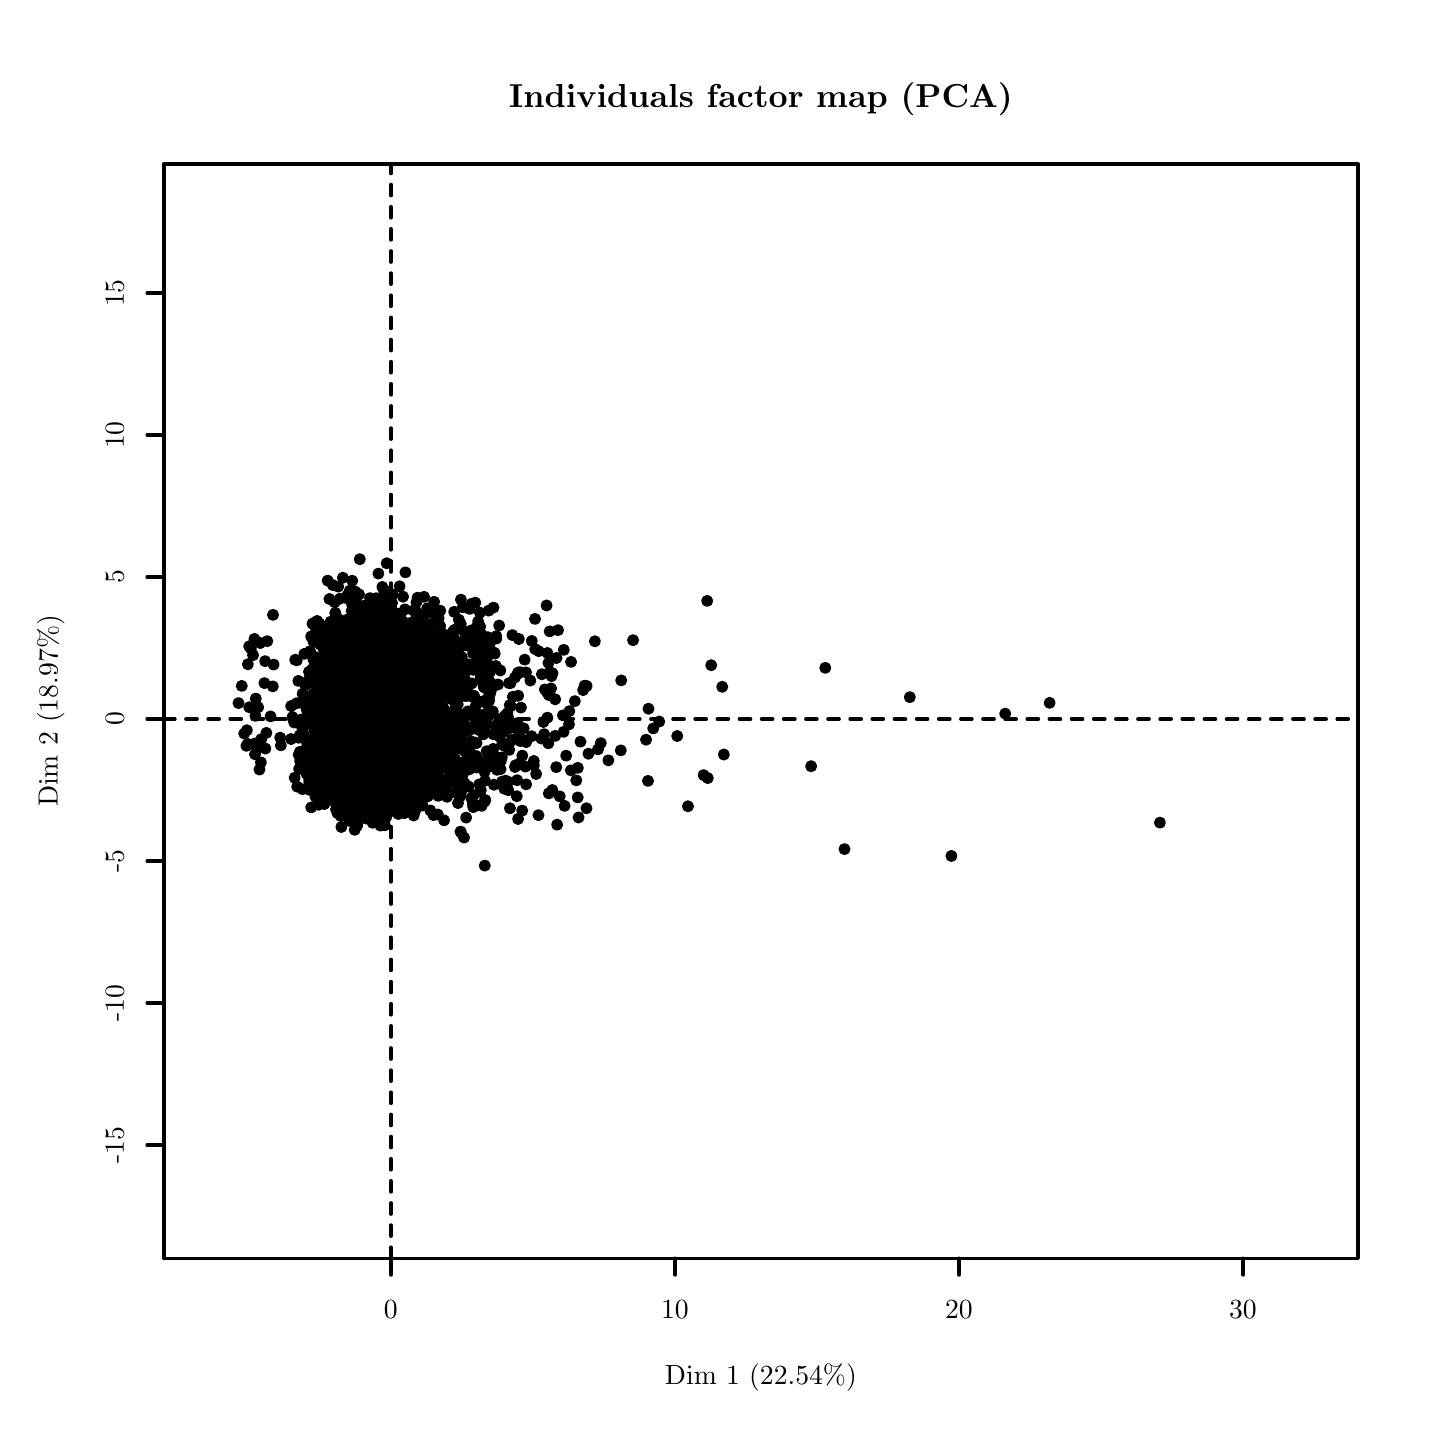
\begin{tikzpicture}[x=1pt,y=1pt]
\definecolor{fillColor}{RGB}{255,255,255}
\path[use as bounding box,fill=fillColor,fill opacity=0.00] (0,0) rectangle (505.89,505.89);
\begin{scope}
\path[clip] ( 49.20, 61.20) rectangle (480.69,456.69);
\definecolor{drawColor}{RGB}{255,255,255}

\path[draw=drawColor,line width= 1.3pt,line join=round,line cap=round] (131.25,256.06) circle (  2.25);
\end{scope}
\begin{scope}
\path[clip] (  0.00,  0.00) rectangle (505.89,505.89);
\definecolor{drawColor}{RGB}{0,0,0}

\path[draw=drawColor,line width= 1.3pt,line join=round,line cap=round] (131.25, 61.20) -- (439.12, 61.20);

\path[draw=drawColor,line width= 1.3pt,line join=round,line cap=round] (131.25, 61.20) -- (131.25, 55.20);

\path[draw=drawColor,line width= 1.3pt,line join=round,line cap=round] (233.88, 61.20) -- (233.88, 55.20);

\path[draw=drawColor,line width= 1.3pt,line join=round,line cap=round] (336.50, 61.20) -- (336.50, 55.20);

\path[draw=drawColor,line width= 1.3pt,line join=round,line cap=round] (439.12, 61.20) -- (439.12, 55.20);

\node[text=drawColor,anchor=base,inner sep=0pt, outer sep=0pt, scale=  1.00] at (131.25, 39.60) {0};

\node[text=drawColor,anchor=base,inner sep=0pt, outer sep=0pt, scale=  1.00] at (233.88, 39.60) {10};

\node[text=drawColor,anchor=base,inner sep=0pt, outer sep=0pt, scale=  1.00] at (336.50, 39.60) {20};

\node[text=drawColor,anchor=base,inner sep=0pt, outer sep=0pt, scale=  1.00] at (439.12, 39.60) {30};

\path[draw=drawColor,line width= 1.3pt,line join=round,line cap=round] ( 49.20,102.13) -- ( 49.20,410.00);

\path[draw=drawColor,line width= 1.3pt,line join=round,line cap=round] ( 49.20,102.13) -- ( 43.20,102.13);

\path[draw=drawColor,line width= 1.3pt,line join=round,line cap=round] ( 49.20,153.44) -- ( 43.20,153.44);

\path[draw=drawColor,line width= 1.3pt,line join=round,line cap=round] ( 49.20,204.75) -- ( 43.20,204.75);

\path[draw=drawColor,line width= 1.3pt,line join=round,line cap=round] ( 49.20,256.06) -- ( 43.20,256.06);

\path[draw=drawColor,line width= 1.3pt,line join=round,line cap=round] ( 49.20,307.37) -- ( 43.20,307.37);

\path[draw=drawColor,line width= 1.3pt,line join=round,line cap=round] ( 49.20,358.69) -- ( 43.20,358.69);

\path[draw=drawColor,line width= 1.3pt,line join=round,line cap=round] ( 49.20,410.00) -- ( 43.20,410.00);

\node[text=drawColor,rotate= 90.00,anchor=base,inner sep=0pt, outer sep=0pt, scale=  1.00] at ( 34.80,102.13) {-15};

\node[text=drawColor,rotate= 90.00,anchor=base,inner sep=0pt, outer sep=0pt, scale=  1.00] at ( 34.80,153.44) {-10};

\node[text=drawColor,rotate= 90.00,anchor=base,inner sep=0pt, outer sep=0pt, scale=  1.00] at ( 34.80,204.75) {-5};

\node[text=drawColor,rotate= 90.00,anchor=base,inner sep=0pt, outer sep=0pt, scale=  1.00] at ( 34.80,256.06) {0};

\node[text=drawColor,rotate= 90.00,anchor=base,inner sep=0pt, outer sep=0pt, scale=  1.00] at ( 34.80,307.37) {5};

\node[text=drawColor,rotate= 90.00,anchor=base,inner sep=0pt, outer sep=0pt, scale=  1.00] at ( 34.80,358.69) {10};

\node[text=drawColor,rotate= 90.00,anchor=base,inner sep=0pt, outer sep=0pt, scale=  1.00] at ( 34.80,410.00) {15};

\path[draw=drawColor,line width= 1.3pt,line join=round,line cap=round] ( 49.20, 61.20) --
	(480.69, 61.20) --
	(480.69,456.69) --
	( 49.20,456.69) --
	( 49.20, 61.20);
\end{scope}
\begin{scope}
\path[clip] (  0.00,  0.00) rectangle (505.89,505.89);
\definecolor{drawColor}{RGB}{0,0,0}

\node[text=drawColor,anchor=base,inner sep=0pt, outer sep=0pt, scale=  1.20] at (264.94,477.15) {\bfseries Individuals factor map (PCA)};

\node[text=drawColor,anchor=base,inner sep=0pt, outer sep=0pt, scale=  1.00] at (264.94, 15.60) {Dim 1 (22.54{\%})};

\node[text=drawColor,rotate= 90.00,anchor=base,inner sep=0pt, outer sep=0pt, scale=  1.00] at ( 10.80,258.94) {Dim 2 (18.97{\%})};
\end{scope}
\begin{scope}
\path[clip] ( 49.20, 61.20) rectangle (480.69,456.69);
\definecolor{drawColor}{RGB}{0,0,0}

\path[draw=drawColor,line width= 1.3pt,dash pattern=on 4pt off 4pt ,line join=round,line cap=round] (131.25, 61.20) -- (131.25,456.69);

\path[draw=drawColor,line width= 1.3pt,dash pattern=on 4pt off 4pt ,line join=round,line cap=round] ( 49.20,256.06) -- (480.69,256.06);
\definecolor{fillColor}{RGB}{0,0,0}

\path[draw=drawColor,line width= 1.3pt,line join=round,line cap=round,fill=fillColor] (130.78,283.63) circle (  1.50);

\path[draw=drawColor,line width= 1.3pt,line join=round,line cap=round,fill=fillColor] (134.72,251.41) circle (  1.50);

\path[draw=drawColor,line width= 1.3pt,line join=round,line cap=round,fill=fillColor] (123.34,270.52) circle (  1.50);

\path[draw=drawColor,line width= 1.3pt,line join=round,line cap=round,fill=fillColor] (134.00,283.88) circle (  1.50);

\path[draw=drawColor,line width= 1.3pt,line join=round,line cap=round,fill=fillColor] (142.96,282.26) circle (  1.50);

\path[draw=drawColor,line width= 1.3pt,line join=round,line cap=round,fill=fillColor] (175.01,248.58) circle (  1.50);

\path[draw=drawColor,line width= 1.3pt,line join=round,line cap=round,fill=fillColor] (170.17,254.61) circle (  1.50);

\path[draw=drawColor,line width= 1.3pt,line join=round,line cap=round,fill=fillColor] (143.32,271.54) circle (  1.50);

\path[draw=drawColor,line width= 1.3pt,line join=round,line cap=round,fill=fillColor] (144.59,263.82) circle (  1.50);

\path[draw=drawColor,line width= 1.3pt,line join=round,line cap=round,fill=fillColor] (142.63,287.61) circle (  1.50);

\path[draw=drawColor,line width= 1.3pt,line join=round,line cap=round,fill=fillColor] (132.01,252.06) circle (  1.50);

\path[draw=drawColor,line width= 1.3pt,line join=round,line cap=round,fill=fillColor] (110.78,269.39) circle (  1.50);

\path[draw=drawColor,line width= 1.3pt,line join=round,line cap=round,fill=fillColor] (118.22,264.41) circle (  1.50);

\path[draw=drawColor,line width= 1.3pt,line join=round,line cap=round,fill=fillColor] (126.69,228.61) circle (  1.50);

\path[draw=drawColor,line width= 1.3pt,line join=round,line cap=round,fill=fillColor] (139.46,269.95) circle (  1.50);

\path[draw=drawColor,line width= 1.3pt,line join=round,line cap=round,fill=fillColor] (142.54,241.49) circle (  1.50);

\path[draw=drawColor,line width= 1.3pt,line join=round,line cap=round,fill=fillColor] (141.94,273.14) circle (  1.50);

\path[draw=drawColor,line width= 1.3pt,line join=round,line cap=round,fill=fillColor] (121.25,263.20) circle (  1.50);

\path[draw=drawColor,line width= 1.3pt,line join=round,line cap=round,fill=fillColor] (157.22,296.44) circle (  1.50);

\path[draw=drawColor,line width= 1.3pt,line join=round,line cap=round,fill=fillColor] (147.90,279.65) circle (  1.50);

\path[draw=drawColor,line width= 1.3pt,line join=round,line cap=round,fill=fillColor] (117.20,248.00) circle (  1.50);

\path[draw=drawColor,line width= 1.3pt,line join=round,line cap=round,fill=fillColor] (128.89,270.01) circle (  1.50);

\path[draw=drawColor,line width= 1.3pt,line join=round,line cap=round,fill=fillColor] (130.27,234.33) circle (  1.50);

\path[draw=drawColor,line width= 1.3pt,line join=round,line cap=round,fill=fillColor] (115.34,226.51) circle (  1.50);

\path[draw=drawColor,line width= 1.3pt,line join=round,line cap=round,fill=fillColor] (146.27,279.47) circle (  1.50);

\path[draw=drawColor,line width= 1.3pt,line join=round,line cap=round,fill=fillColor] (131.76,255.75) circle (  1.50);

\path[draw=drawColor,line width= 1.3pt,line join=round,line cap=round,fill=fillColor] (156.98,283.84) circle (  1.50);

\path[draw=drawColor,line width= 1.3pt,line join=round,line cap=round,fill=fillColor] (140.75,251.49) circle (  1.50);

\path[draw=drawColor,line width= 1.3pt,line join=round,line cap=round,fill=fillColor] (141.38,247.43) circle (  1.50);

\path[draw=drawColor,line width= 1.3pt,line join=round,line cap=round,fill=fillColor] (137.27,260.43) circle (  1.50);

\path[draw=drawColor,line width= 1.3pt,line join=round,line cap=round,fill=fillColor] (139.30,270.61) circle (  1.50);

\path[draw=drawColor,line width= 1.3pt,line join=round,line cap=round,fill=fillColor] (139.77,263.23) circle (  1.50);

\path[draw=drawColor,line width= 1.3pt,line join=round,line cap=round,fill=fillColor] (125.75,237.27) circle (  1.50);

\path[draw=drawColor,line width= 1.3pt,line join=round,line cap=round,fill=fillColor] (148.56,241.91) circle (  1.50);

\path[draw=drawColor,line width= 1.3pt,line join=round,line cap=round,fill=fillColor] (140.79,267.47) circle (  1.50);

\path[draw=drawColor,line width= 1.3pt,line join=round,line cap=round,fill=fillColor] (166.68,259.24) circle (  1.50);

\path[draw=drawColor,line width= 1.3pt,line join=round,line cap=round,fill=fillColor] (142.03,267.66) circle (  1.50);

\path[draw=drawColor,line width= 1.3pt,line join=round,line cap=round,fill=fillColor] (173.95,269.03) circle (  1.50);

\path[draw=drawColor,line width= 1.3pt,line join=round,line cap=round,fill=fillColor] (178.73,242.84) circle (  1.50);

\path[draw=drawColor,line width= 1.3pt,line join=round,line cap=round,fill=fillColor] (144.56,260.02) circle (  1.50);

\path[draw=drawColor,line width= 1.3pt,line join=round,line cap=round,fill=fillColor] (143.44,282.08) circle (  1.50);

\path[draw=drawColor,line width= 1.3pt,line join=round,line cap=round,fill=fillColor] (133.52,234.34) circle (  1.50);

\path[draw=drawColor,line width= 1.3pt,line join=round,line cap=round,fill=fillColor] (132.88,270.54) circle (  1.50);

\path[draw=drawColor,line width= 1.3pt,line join=round,line cap=round,fill=fillColor] (113.26,256.27) circle (  1.50);

\path[draw=drawColor,line width= 1.3pt,line join=round,line cap=round,fill=fillColor] (128.72,282.44) circle (  1.50);

\path[draw=drawColor,line width= 1.3pt,line join=round,line cap=round,fill=fillColor] (160.58,257.25) circle (  1.50);

\path[draw=drawColor,line width= 1.3pt,line join=round,line cap=round,fill=fillColor] (137.11,271.86) circle (  1.50);

\path[draw=drawColor,line width= 1.3pt,line join=round,line cap=round,fill=fillColor] (144.26,243.36) circle (  1.50);

\path[draw=drawColor,line width= 1.3pt,line join=round,line cap=round,fill=fillColor] (177.49,253.59) circle (  1.50);

\path[draw=drawColor,line width= 1.3pt,line join=round,line cap=round,fill=fillColor] (126.41,264.08) circle (  1.50);

\path[draw=drawColor,line width= 1.3pt,line join=round,line cap=round,fill=fillColor] (142.21,252.84) circle (  1.50);

\path[draw=drawColor,line width= 1.3pt,line join=round,line cap=round,fill=fillColor] (122.31,254.07) circle (  1.50);

\path[draw=drawColor,line width= 1.3pt,line join=round,line cap=round,fill=fillColor] (138.52,222.60) circle (  1.50);

\path[draw=drawColor,line width= 1.3pt,line join=round,line cap=round,fill=fillColor] (162.63,281.45) circle (  1.50);

\path[draw=drawColor,line width= 1.3pt,line join=round,line cap=round,fill=fillColor] (128.80,280.03) circle (  1.50);

\path[draw=drawColor,line width= 1.3pt,line join=round,line cap=round,fill=fillColor] (123.49,243.02) circle (  1.50);

\path[draw=drawColor,line width= 1.3pt,line join=round,line cap=round,fill=fillColor] (178.24,260.20) circle (  1.50);

\path[draw=drawColor,line width= 1.3pt,line join=round,line cap=round,fill=fillColor] (139.47,267.30) circle (  1.50);

\path[draw=drawColor,line width= 1.3pt,line join=round,line cap=round,fill=fillColor] (124.72,288.51) circle (  1.50);

\path[draw=drawColor,line width= 1.3pt,line join=round,line cap=round,fill=fillColor] (116.81,246.64) circle (  1.50);

\path[draw=drawColor,line width= 1.3pt,line join=round,line cap=round,fill=fillColor] (142.37,277.54) circle (  1.50);

\path[draw=drawColor,line width= 1.3pt,line join=round,line cap=round,fill=fillColor] (140.27,284.15) circle (  1.50);

\path[draw=drawColor,line width= 1.3pt,line join=round,line cap=round,fill=fillColor] (136.68,259.45) circle (  1.50);

\path[draw=drawColor,line width= 1.3pt,line join=round,line cap=round,fill=fillColor] (142.08,274.79) circle (  1.50);

\path[draw=drawColor,line width= 1.3pt,line join=round,line cap=round,fill=fillColor] (142.37,252.20) circle (  1.50);

\path[draw=drawColor,line width= 1.3pt,line join=round,line cap=round,fill=fillColor] (162.13,289.12) circle (  1.50);

\path[draw=drawColor,line width= 1.3pt,line join=round,line cap=round,fill=fillColor] (155.44,249.72) circle (  1.50);

\path[draw=drawColor,line width= 1.3pt,line join=round,line cap=round,fill=fillColor] (153.35,263.12) circle (  1.50);

\path[draw=drawColor,line width= 1.3pt,line join=round,line cap=round,fill=fillColor] (128.89,250.74) circle (  1.50);

\path[draw=drawColor,line width= 1.3pt,line join=round,line cap=round,fill=fillColor] (148.55,269.91) circle (  1.50);

\path[draw=drawColor,line width= 1.3pt,line join=round,line cap=round,fill=fillColor] (142.42,287.68) circle (  1.50);

\path[draw=drawColor,line width= 1.3pt,line join=round,line cap=round,fill=fillColor] (138.06,254.03) circle (  1.50);

\path[draw=drawColor,line width= 1.3pt,line join=round,line cap=round,fill=fillColor] (114.55,290.17) circle (  1.50);

\path[draw=drawColor,line width= 1.3pt,line join=round,line cap=round,fill=fillColor] (126.59,223.38) circle (  1.50);

\path[draw=drawColor,line width= 1.3pt,line join=round,line cap=round,fill=fillColor] (141.40,259.49) circle (  1.50);

\path[draw=drawColor,line width= 1.3pt,line join=round,line cap=round,fill=fillColor] (133.92,221.76) circle (  1.50);

\path[draw=drawColor,line width= 1.3pt,line join=round,line cap=round,fill=fillColor] (141.43,276.14) circle (  1.50);

\path[draw=drawColor,line width= 1.3pt,line join=round,line cap=round,fill=fillColor] (179.24,252.68) circle (  1.50);

\path[draw=drawColor,line width= 1.3pt,line join=round,line cap=round,fill=fillColor] (155.15,229.30) circle (  1.50);

\path[draw=drawColor,line width= 1.3pt,line join=round,line cap=round,fill=fillColor] (127.83,274.49) circle (  1.50);

\path[draw=drawColor,line width= 1.3pt,line join=round,line cap=round,fill=fillColor] (139.69,278.69) circle (  1.50);

\path[draw=drawColor,line width= 1.3pt,line join=round,line cap=round,fill=fillColor] (130.78,253.32) circle (  1.50);

\path[draw=drawColor,line width= 1.3pt,line join=round,line cap=round,fill=fillColor] (141.22,272.16) circle (  1.50);

\path[draw=drawColor,line width= 1.3pt,line join=round,line cap=round,fill=fillColor] (140.58,292.91) circle (  1.50);

\path[draw=drawColor,line width= 1.3pt,line join=round,line cap=round,fill=fillColor] (142.06,293.66) circle (  1.50);

\path[draw=drawColor,line width= 1.3pt,line join=round,line cap=round,fill=fillColor] (163.16,285.46) circle (  1.50);

\path[draw=drawColor,line width= 1.3pt,line join=round,line cap=round,fill=fillColor] (119.62,235.09) circle (  1.50);

\path[draw=drawColor,line width= 1.3pt,line join=round,line cap=round,fill=fillColor] (129.88,239.08) circle (  1.50);

\path[draw=drawColor,line width= 1.3pt,line join=round,line cap=round,fill=fillColor] (160.40,297.69) circle (  1.50);

\path[draw=drawColor,line width= 1.3pt,line join=round,line cap=round,fill=fillColor] (112.86,266.88) circle (  1.50);

\path[draw=drawColor,line width= 1.3pt,line join=round,line cap=round,fill=fillColor] (159.50,273.91) circle (  1.50);

\path[draw=drawColor,line width= 1.3pt,line join=round,line cap=round,fill=fillColor] (145.34,270.68) circle (  1.50);

\path[draw=drawColor,line width= 1.3pt,line join=round,line cap=round,fill=fillColor] (100.71,236.40) circle (  1.50);

\path[draw=drawColor,line width= 1.3pt,line join=round,line cap=round,fill=fillColor] (115.38,272.45) circle (  1.50);

\path[draw=drawColor,line width= 1.3pt,line join=round,line cap=round,fill=fillColor] ( 79.57,275.86) circle (  1.50);

\path[draw=drawColor,line width= 1.3pt,line join=round,line cap=round,fill=fillColor] (108.26,281.93) circle (  1.50);

\path[draw=drawColor,line width= 1.3pt,line join=round,line cap=round,fill=fillColor] (123.79,264.20) circle (  1.50);

\path[draw=drawColor,line width= 1.3pt,line join=round,line cap=round,fill=fillColor] (127.72,230.76) circle (  1.50);

\path[draw=drawColor,line width= 1.3pt,line join=round,line cap=round,fill=fillColor] ( 85.56,269.06) circle (  1.50);

\path[draw=drawColor,line width= 1.3pt,line join=round,line cap=round,fill=fillColor] (144.97,270.20) circle (  1.50);

\path[draw=drawColor,line width= 1.3pt,line join=round,line cap=round,fill=fillColor] (136.47,277.63) circle (  1.50);

\path[draw=drawColor,line width= 1.3pt,line join=round,line cap=round,fill=fillColor] ( 80.06,282.35) circle (  1.50);

\path[draw=drawColor,line width= 1.3pt,line join=round,line cap=round,fill=fillColor] (125.90,276.67) circle (  1.50);

\path[draw=drawColor,line width= 1.3pt,line join=round,line cap=round,fill=fillColor] (161.05,273.81) circle (  1.50);

\path[draw=drawColor,line width= 1.3pt,line join=round,line cap=round,fill=fillColor] ( 86.26,251.05) circle (  1.50);

\path[draw=drawColor,line width= 1.3pt,line join=round,line cap=round,fill=fillColor] (226.06,252.67) circle (  1.50);

\path[draw=drawColor,line width= 1.3pt,line join=round,line cap=round,fill=fillColor] ( 81.95,285.00) circle (  1.50);

\path[draw=drawColor,line width= 1.3pt,line join=round,line cap=round,fill=fillColor] (138.64,283.33) circle (  1.50);

\path[draw=drawColor,line width= 1.3pt,line join=round,line cap=round,fill=fillColor] ( 86.59,284.22) circle (  1.50);

\path[draw=drawColor,line width= 1.3pt,line join=round,line cap=round,fill=fillColor] (136.67,266.02) circle (  1.50);

\path[draw=drawColor,line width= 1.3pt,line join=round,line cap=round,fill=fillColor] (107.55,287.94) circle (  1.50);

\path[draw=drawColor,line width= 1.3pt,line join=round,line cap=round,fill=fillColor] (128.91,252.01) circle (  1.50);

\path[draw=drawColor,line width= 1.3pt,line join=round,line cap=round,fill=fillColor] (108.56,246.38) circle (  1.50);

\path[draw=drawColor,line width= 1.3pt,line join=round,line cap=round,fill=fillColor] (105.62,250.16) circle (  1.50);

\path[draw=drawColor,line width= 1.3pt,line join=round,line cap=round,fill=fillColor] ( 95.17,248.83) circle (  1.50);

\path[draw=drawColor,line width= 1.3pt,line join=round,line cap=round,fill=fillColor] ( 91.49,246.54) circle (  1.50);

\path[draw=drawColor,line width= 1.3pt,line join=round,line cap=round,fill=fillColor] (108.18,249.12) circle (  1.50);

\path[draw=drawColor,line width= 1.3pt,line join=round,line cap=round,fill=fillColor] (138.66,258.92) circle (  1.50);

\path[draw=drawColor,line width= 1.3pt,line join=round,line cap=round,fill=fillColor] (138.74,290.75) circle (  1.50);

\path[draw=drawColor,line width= 1.3pt,line join=round,line cap=round,fill=fillColor] (116.45,254.69) circle (  1.50);

\path[draw=drawColor,line width= 1.3pt,line join=round,line cap=round,fill=fillColor] (137.06,276.79) circle (  1.50);

\path[draw=drawColor,line width= 1.3pt,line join=round,line cap=round,fill=fillColor] ( 80.07,260.33) circle (  1.50);

\path[draw=drawColor,line width= 1.3pt,line join=round,line cap=round,fill=fillColor] (122.72,245.66) circle (  1.50);

\path[draw=drawColor,line width= 1.3pt,line join=round,line cap=round,fill=fillColor] (125.06,285.84) circle (  1.50);

\path[draw=drawColor,line width= 1.3pt,line join=round,line cap=round,fill=fillColor] (143.64,284.12) circle (  1.50);

\path[draw=drawColor,line width= 1.3pt,line join=round,line cap=round,fill=fillColor] ( 79.56,247.04) circle (  1.50);

\path[draw=drawColor,line width= 1.3pt,line join=round,line cap=round,fill=fillColor] (125.01,249.18) circle (  1.50);

\path[draw=drawColor,line width= 1.3pt,line join=round,line cap=round,fill=fillColor] ( 83.29,260.31) circle (  1.50);

\path[draw=drawColor,line width= 1.3pt,line join=round,line cap=round,fill=fillColor] (138.31,287.06) circle (  1.50);

\path[draw=drawColor,line width= 1.3pt,line join=round,line cap=round,fill=fillColor] (150.75,263.90) circle (  1.50);

\path[draw=drawColor,line width= 1.3pt,line join=round,line cap=round,fill=fillColor] (108.12,267.22) circle (  1.50);

\path[draw=drawColor,line width= 1.3pt,line join=round,line cap=round,fill=fillColor] (123.85,284.44) circle (  1.50);

\path[draw=drawColor,line width= 1.3pt,line join=round,line cap=round,fill=fillColor] (130.95,257.20) circle (  1.50);

\path[draw=drawColor,line width= 1.3pt,line join=round,line cap=round,fill=fillColor] (140.20,245.81) circle (  1.50);

\path[draw=drawColor,line width= 1.3pt,line join=round,line cap=round,fill=fillColor] (112.76,235.65) circle (  1.50);

\path[draw=drawColor,line width= 1.3pt,line join=round,line cap=round,fill=fillColor] (115.80,266.50) circle (  1.50);

\path[draw=drawColor,line width= 1.3pt,line join=round,line cap=round,fill=fillColor] (137.11,279.21) circle (  1.50);

\path[draw=drawColor,line width= 1.3pt,line join=round,line cap=round,fill=fillColor] ( 79.21,252.03) circle (  1.50);

\path[draw=drawColor,line width= 1.3pt,line join=round,line cap=round,fill=fillColor] (121.11,288.06) circle (  1.50);

\path[draw=drawColor,line width= 1.3pt,line join=round,line cap=round,fill=fillColor] (136.13,285.12) circle (  1.50);

\path[draw=drawColor,line width= 1.3pt,line join=round,line cap=round,fill=fillColor] (114.84,258.02) circle (  1.50);

\path[draw=drawColor,line width= 1.3pt,line join=round,line cap=round,fill=fillColor] ( 84.05,283.54) circle (  1.50);

\path[draw=drawColor,line width= 1.3pt,line join=round,line cap=round,fill=fillColor] (144.38,296.07) circle (  1.50);

\path[draw=drawColor,line width= 1.3pt,line join=round,line cap=round,fill=fillColor] (127.58,296.18) circle (  1.50);

\path[draw=drawColor,line width= 1.3pt,line join=round,line cap=round,fill=fillColor] (139.31,264.69) circle (  1.50);

\path[draw=drawColor,line width= 1.3pt,line join=round,line cap=round,fill=fillColor] ( 83.85,245.98) circle (  1.50);

\path[draw=drawColor,line width= 1.3pt,line join=round,line cap=round,fill=fillColor] ( 81.44,279.16) circle (  1.50);

\path[draw=drawColor,line width= 1.3pt,line join=round,line cap=round,fill=fillColor] (154.69,261.12) circle (  1.50);

\path[draw=drawColor,line width= 1.3pt,line join=round,line cap=round,fill=fillColor] (117.36,248.70) circle (  1.50);

\path[draw=drawColor,line width= 1.3pt,line join=round,line cap=round,fill=fillColor] (118.40,240.41) circle (  1.50);

\path[draw=drawColor,line width= 1.3pt,line join=round,line cap=round,fill=fillColor] ( 83.76,237.82) circle (  1.50);

\path[draw=drawColor,line width= 1.3pt,line join=round,line cap=round,fill=fillColor] (131.67,237.67) circle (  1.50);

\path[draw=drawColor,line width= 1.3pt,line join=round,line cap=round,fill=fillColor] ( 87.77,257.02) circle (  1.50);

\path[draw=drawColor,line width= 1.3pt,line join=round,line cap=round,fill=fillColor] (144.04,294.20) circle (  1.50);

\path[draw=drawColor,line width= 1.3pt,line join=round,line cap=round,fill=fillColor] (141.16,260.05) circle (  1.50);

\path[draw=drawColor,line width= 1.3pt,line join=round,line cap=round,fill=fillColor] ( 82.71,246.13) circle (  1.50);

\path[draw=drawColor,line width= 1.3pt,line join=round,line cap=round,fill=fillColor] (100.86,259.51) circle (  1.50);

\path[draw=drawColor,line width= 1.3pt,line join=round,line cap=round,fill=fillColor] (140.88,255.59) circle (  1.50);

\path[draw=drawColor,line width= 1.3pt,line join=round,line cap=round,fill=fillColor] (159.19,275.80) circle (  1.50);

\path[draw=drawColor,line width= 1.3pt,line join=round,line cap=round,fill=fillColor] (129.50,261.64) circle (  1.50);

\path[draw=drawColor,line width= 1.3pt,line join=round,line cap=round,fill=fillColor] (142.55,289.24) circle (  1.50);

\path[draw=drawColor,line width= 1.3pt,line join=round,line cap=round,fill=fillColor] (131.80,267.20) circle (  1.50);

\path[draw=drawColor,line width= 1.3pt,line join=round,line cap=round,fill=fillColor] (162.76,291.35) circle (  1.50);

\path[draw=drawColor,line width= 1.3pt,line join=round,line cap=round,fill=fillColor] (137.32,272.55) circle (  1.50);

\path[draw=drawColor,line width= 1.3pt,line join=round,line cap=round,fill=fillColor] (175.14,286.40) circle (  1.50);

\path[draw=drawColor,line width= 1.3pt,line join=round,line cap=round,fill=fillColor] ( 80.66,281.51) circle (  1.50);

\path[draw=drawColor,line width= 1.3pt,line join=round,line cap=round,fill=fillColor] (147.11,276.30) circle (  1.50);

\path[draw=drawColor,line width= 1.3pt,line join=round,line cap=round,fill=fillColor] ( 97.26,277.28) circle (  1.50);

\path[draw=drawColor,line width= 1.3pt,line join=round,line cap=round,fill=fillColor] (168.77,279.68) circle (  1.50);

\path[draw=drawColor,line width= 1.3pt,line join=round,line cap=round,fill=fillColor] (112.51,224.01) circle (  1.50);

\path[draw=drawColor,line width= 1.3pt,line join=round,line cap=round,fill=fillColor] (161.74,298.11) circle (  1.50);

\path[draw=drawColor,line width= 1.3pt,line join=round,line cap=round,fill=fillColor] (135.64,250.55) circle (  1.50);

\path[draw=drawColor,line width= 1.3pt,line join=round,line cap=round,fill=fillColor] (137.65,266.83) circle (  1.50);

\path[draw=drawColor,line width= 1.3pt,line join=round,line cap=round,fill=fillColor] (147.60,264.21) circle (  1.50);

\path[draw=drawColor,line width= 1.3pt,line join=round,line cap=round,fill=fillColor] (125.32,299.47) circle (  1.50);

\path[draw=drawColor,line width= 1.3pt,line join=round,line cap=round,fill=fillColor] ( 82.15,243.34) circle (  1.50);

\path[draw=drawColor,line width= 1.3pt,line join=round,line cap=round,fill=fillColor] (136.82,276.42) circle (  1.50);

\path[draw=drawColor,line width= 1.3pt,line join=round,line cap=round,fill=fillColor] (164.76,267.80) circle (  1.50);

\path[draw=drawColor,line width= 1.3pt,line join=round,line cap=round,fill=fillColor] (224.33,259.79) circle (  1.50);

\path[draw=drawColor,line width= 1.3pt,line join=round,line cap=round,fill=fillColor] (126.89,283.78) circle (  1.50);

\path[draw=drawColor,line width= 1.3pt,line join=round,line cap=round,fill=fillColor] (156.55,299.21) circle (  1.50);

\path[draw=drawColor,line width= 1.3pt,line join=round,line cap=round,fill=fillColor] (109.23,236.67) circle (  1.50);

\path[draw=drawColor,line width= 1.3pt,line join=round,line cap=round,fill=fillColor] (130.85,274.79) circle (  1.50);

\path[draw=drawColor,line width= 1.3pt,line join=round,line cap=round,fill=fillColor] (126.14,274.84) circle (  1.50);

\path[draw=drawColor,line width= 1.3pt,line join=round,line cap=round,fill=fillColor] (113.37,291.67) circle (  1.50);

\path[draw=drawColor,line width= 1.3pt,line join=round,line cap=round,fill=fillColor] (143.45,238.20) circle (  1.50);

\path[draw=drawColor,line width= 1.3pt,line join=round,line cap=round,fill=fillColor] (151.30,268.24) circle (  1.50);

\path[draw=drawColor,line width= 1.3pt,line join=round,line cap=round,fill=fillColor] (126.49,272.85) circle (  1.50);

\path[draw=drawColor,line width= 1.3pt,line join=round,line cap=round,fill=fillColor] (120.40,274.72) circle (  1.50);

\path[draw=drawColor,line width= 1.3pt,line join=round,line cap=round,fill=fillColor] (141.24,243.45) circle (  1.50);

\path[draw=drawColor,line width= 1.3pt,line join=round,line cap=round,fill=fillColor] (129.74,234.95) circle (  1.50);

\path[draw=drawColor,line width= 1.3pt,line join=round,line cap=round,fill=fillColor] (137.77,278.73) circle (  1.50);

\path[draw=drawColor,line width= 1.3pt,line join=round,line cap=round,fill=fillColor] (119.82,235.41) circle (  1.50);

\path[draw=drawColor,line width= 1.3pt,line join=round,line cap=round,fill=fillColor] (131.36,288.05) circle (  1.50);

\path[draw=drawColor,line width= 1.3pt,line join=round,line cap=round,fill=fillColor] (110.53,289.97) circle (  1.50);

\path[draw=drawColor,line width= 1.3pt,line join=round,line cap=round,fill=fillColor] (137.01,287.66) circle (  1.50);

\path[draw=drawColor,line width= 1.3pt,line join=round,line cap=round,fill=fillColor] (128.25,235.34) circle (  1.50);

\path[draw=drawColor,line width= 1.3pt,line join=round,line cap=round,fill=fillColor] (116.00,290.56) circle (  1.50);

\path[draw=drawColor,line width= 1.3pt,line join=round,line cap=round,fill=fillColor] (136.06,267.77) circle (  1.50);

\path[draw=drawColor,line width= 1.3pt,line join=round,line cap=round,fill=fillColor] (131.71,283.41) circle (  1.50);

\path[draw=drawColor,line width= 1.3pt,line join=round,line cap=round,fill=fillColor] (189.28,271.56) circle (  1.50);

\path[draw=drawColor,line width= 1.3pt,line join=round,line cap=round,fill=fillColor] (121.30,221.32) circle (  1.50);

\path[draw=drawColor,line width= 1.3pt,line join=round,line cap=round,fill=fillColor] (119.57,293.77) circle (  1.50);

\path[draw=drawColor,line width= 1.3pt,line join=round,line cap=round,fill=fillColor] (127.85,276.69) circle (  1.50);

\path[draw=drawColor,line width= 1.3pt,line join=round,line cap=round,fill=fillColor] (141.39,260.55) circle (  1.50);

\path[draw=drawColor,line width= 1.3pt,line join=round,line cap=round,fill=fillColor] (123.26,276.59) circle (  1.50);

\path[draw=drawColor,line width= 1.3pt,line join=round,line cap=round,fill=fillColor] (137.43,247.54) circle (  1.50);

\path[draw=drawColor,line width= 1.3pt,line join=round,line cap=round,fill=fillColor] (149.73,282.45) circle (  1.50);

\path[draw=drawColor,line width= 1.3pt,line join=round,line cap=round,fill=fillColor] (132.22,276.22) circle (  1.50);

\path[draw=drawColor,line width= 1.3pt,line join=round,line cap=round,fill=fillColor] (115.39,238.83) circle (  1.50);

\path[draw=drawColor,line width= 1.3pt,line join=round,line cap=round,fill=fillColor] (150.82,245.02) circle (  1.50);

\path[draw=drawColor,line width= 1.3pt,line join=round,line cap=round,fill=fillColor] (137.50,281.78) circle (  1.50);

\path[draw=drawColor,line width= 1.3pt,line join=round,line cap=round,fill=fillColor] (163.91,240.12) circle (  1.50);

\path[draw=drawColor,line width= 1.3pt,line join=round,line cap=round,fill=fillColor] (122.72,275.59) circle (  1.50);

\path[draw=drawColor,line width= 1.3pt,line join=round,line cap=round,fill=fillColor] (129.04,244.12) circle (  1.50);

\path[draw=drawColor,line width= 1.3pt,line join=round,line cap=round,fill=fillColor] (164.71,257.61) circle (  1.50);

\path[draw=drawColor,line width= 1.3pt,line join=round,line cap=round,fill=fillColor] (120.05,244.70) circle (  1.50);

\path[draw=drawColor,line width= 1.3pt,line join=round,line cap=round,fill=fillColor] (135.45,281.90) circle (  1.50);

\path[draw=drawColor,line width= 1.3pt,line join=round,line cap=round,fill=fillColor] (120.57,250.96) circle (  1.50);

\path[draw=drawColor,line width= 1.3pt,line join=round,line cap=round,fill=fillColor] (150.66,255.81) circle (  1.50);

\path[draw=drawColor,line width= 1.3pt,line join=round,line cap=round,fill=fillColor] (117.76,266.09) circle (  1.50);

\path[draw=drawColor,line width= 1.3pt,line join=round,line cap=round,fill=fillColor] (129.03,255.25) circle (  1.50);

\path[draw=drawColor,line width= 1.3pt,line join=round,line cap=round,fill=fillColor] (137.50,257.88) circle (  1.50);

\path[draw=drawColor,line width= 1.3pt,line join=round,line cap=round,fill=fillColor] (118.73,251.88) circle (  1.50);

\path[draw=drawColor,line width= 1.3pt,line join=round,line cap=round,fill=fillColor] (124.41,287.01) circle (  1.50);

\path[draw=drawColor,line width= 1.3pt,line join=round,line cap=round,fill=fillColor] (111.53,239.66) circle (  1.50);

\path[draw=drawColor,line width= 1.3pt,line join=round,line cap=round,fill=fillColor] (115.36,241.48) circle (  1.50);

\path[draw=drawColor,line width= 1.3pt,line join=round,line cap=round,fill=fillColor] (120.58,250.37) circle (  1.50);

\path[draw=drawColor,line width= 1.3pt,line join=round,line cap=round,fill=fillColor] (124.99,235.53) circle (  1.50);

\path[draw=drawColor,line width= 1.3pt,line join=round,line cap=round,fill=fillColor] (151.30,283.77) circle (  1.50);

\path[draw=drawColor,line width= 1.3pt,line join=round,line cap=round,fill=fillColor] (114.11,243.46) circle (  1.50);

\path[draw=drawColor,line width= 1.3pt,line join=round,line cap=round,fill=fillColor] (139.30,259.08) circle (  1.50);

\path[draw=drawColor,line width= 1.3pt,line join=round,line cap=round,fill=fillColor] (127.32,293.84) circle (  1.50);

\path[draw=drawColor,line width= 1.3pt,line join=round,line cap=round,fill=fillColor] (112.50,273.49) circle (  1.50);

\path[draw=drawColor,line width= 1.3pt,line join=round,line cap=round,fill=fillColor] (127.58,257.84) circle (  1.50);

\path[draw=drawColor,line width= 1.3pt,line join=round,line cap=round,fill=fillColor] (129.86,285.89) circle (  1.50);

\path[draw=drawColor,line width= 1.3pt,line join=round,line cap=round,fill=fillColor] (125.41,239.05) circle (  1.50);

\path[draw=drawColor,line width= 1.3pt,line join=round,line cap=round,fill=fillColor] (112.95,267.81) circle (  1.50);

\path[draw=drawColor,line width= 1.3pt,line join=round,line cap=round,fill=fillColor] (150.57,253.48) circle (  1.50);

\path[draw=drawColor,line width= 1.3pt,line join=round,line cap=round,fill=fillColor] (141.65,265.80) circle (  1.50);

\path[draw=drawColor,line width= 1.3pt,line join=round,line cap=round,fill=fillColor] (122.14,224.30) circle (  1.50);

\path[draw=drawColor,line width= 1.3pt,line join=round,line cap=round,fill=fillColor] (144.74,245.43) circle (  1.50);

\path[draw=drawColor,line width= 1.3pt,line join=round,line cap=round,fill=fillColor] (228.21,255.15) circle (  1.50);

\path[draw=drawColor,line width= 1.3pt,line join=round,line cap=round,fill=fillColor] (149.82,286.99) circle (  1.50);

\path[draw=drawColor,line width= 1.3pt,line join=round,line cap=round,fill=fillColor] (147.31,248.61) circle (  1.50);

\path[draw=drawColor,line width= 1.3pt,line join=round,line cap=round,fill=fillColor] (194.58,242.83) circle (  1.50);

\path[draw=drawColor,line width= 1.3pt,line join=round,line cap=round,fill=fillColor] (109.95,239.73) circle (  1.50);

\path[draw=drawColor,line width= 1.3pt,line join=round,line cap=round,fill=fillColor] (119.19,256.62) circle (  1.50);

\path[draw=drawColor,line width= 1.3pt,line join=round,line cap=round,fill=fillColor] (168.30,250.55) circle (  1.50);

\path[draw=drawColor,line width= 1.3pt,line join=round,line cap=round,fill=fillColor] (121.95,280.74) circle (  1.50);

\path[draw=drawColor,line width= 1.3pt,line join=round,line cap=round,fill=fillColor] (119.02,274.65) circle (  1.50);

\path[draw=drawColor,line width= 1.3pt,line join=round,line cap=round,fill=fillColor] (137.61,233.86) circle (  1.50);

\path[draw=drawColor,line width= 1.3pt,line join=round,line cap=round,fill=fillColor] (120.07,258.52) circle (  1.50);

\path[draw=drawColor,line width= 1.3pt,line join=round,line cap=round,fill=fillColor] (132.76,237.62) circle (  1.50);

\path[draw=drawColor,line width= 1.3pt,line join=round,line cap=round,fill=fillColor] (127.24,277.01) circle (  1.50);

\path[draw=drawColor,line width= 1.3pt,line join=round,line cap=round,fill=fillColor] (109.17,260.51) circle (  1.50);

\path[draw=drawColor,line width= 1.3pt,line join=round,line cap=round,fill=fillColor] (125.01,257.87) circle (  1.50);

\path[draw=drawColor,line width= 1.3pt,line join=round,line cap=round,fill=fillColor] (117.66,279.03) circle (  1.50);

\path[draw=drawColor,line width= 1.3pt,line join=round,line cap=round,fill=fillColor] (141.62,272.31) circle (  1.50);

\path[draw=drawColor,line width= 1.3pt,line join=round,line cap=round,fill=fillColor] (122.95,261.62) circle (  1.50);

\path[draw=drawColor,line width= 1.3pt,line join=round,line cap=round,fill=fillColor] (143.42,231.86) circle (  1.50);

\path[draw=drawColor,line width= 1.3pt,line join=round,line cap=round,fill=fillColor] (126.57,248.90) circle (  1.50);

\path[draw=drawColor,line width= 1.3pt,line join=round,line cap=round,fill=fillColor] (123.39,227.49) circle (  1.50);

\path[draw=drawColor,line width= 1.3pt,line join=round,line cap=round,fill=fillColor] (129.43,247.38) circle (  1.50);

\path[draw=drawColor,line width= 1.3pt,line join=round,line cap=round,fill=fillColor] (166.67,263.66) circle (  1.50);

\path[draw=drawColor,line width= 1.3pt,line join=round,line cap=round,fill=fillColor] (147.57,250.32) circle (  1.50);

\path[draw=drawColor,line width= 1.3pt,line join=round,line cap=round,fill=fillColor] (113.14,240.15) circle (  1.50);

\path[draw=drawColor,line width= 1.3pt,line join=round,line cap=round,fill=fillColor] (147.29,246.23) circle (  1.50);

\path[draw=drawColor,line width= 1.3pt,line join=round,line cap=round,fill=fillColor] (124.80,269.37) circle (  1.50);

\path[draw=drawColor,line width= 1.3pt,line join=round,line cap=round,fill=fillColor] (111.46,254.02) circle (  1.50);

\path[draw=drawColor,line width= 1.3pt,line join=round,line cap=round,fill=fillColor] (115.19,243.63) circle (  1.50);

\path[draw=drawColor,line width= 1.3pt,line join=round,line cap=round,fill=fillColor] (119.84,253.34) circle (  1.50);

\path[draw=drawColor,line width= 1.3pt,line join=round,line cap=round,fill=fillColor] (112.96,258.65) circle (  1.50);

\path[draw=drawColor,line width= 1.3pt,line join=round,line cap=round,fill=fillColor] (123.87,272.74) circle (  1.50);

\path[draw=drawColor,line width= 1.3pt,line join=round,line cap=round,fill=fillColor] (130.57,243.63) circle (  1.50);

\path[draw=drawColor,line width= 1.3pt,line join=round,line cap=round,fill=fillColor] (148.32,234.05) circle (  1.50);

\path[draw=drawColor,line width= 1.3pt,line join=round,line cap=round,fill=fillColor] (117.75,290.08) circle (  1.50);

\path[draw=drawColor,line width= 1.3pt,line join=round,line cap=round,fill=fillColor] (143.70,248.64) circle (  1.50);

\path[draw=drawColor,line width= 1.3pt,line join=round,line cap=round,fill=fillColor] (109.85,226.96) circle (  1.50);

\path[draw=drawColor,line width= 1.3pt,line join=round,line cap=round,fill=fillColor] (134.51,249.32) circle (  1.50);

\path[draw=drawColor,line width= 1.3pt,line join=round,line cap=round,fill=fillColor] (106.40,231.29) circle (  1.50);

\path[draw=drawColor,line width= 1.3pt,line join=round,line cap=round,fill=fillColor] (163.73,230.32) circle (  1.50);

\path[draw=drawColor,line width= 1.3pt,line join=round,line cap=round,fill=fillColor] (114.57,243.44) circle (  1.50);

\path[draw=drawColor,line width= 1.3pt,line join=round,line cap=round,fill=fillColor] (177.05,272.35) circle (  1.50);

\path[draw=drawColor,line width= 1.3pt,line join=round,line cap=round,fill=fillColor] (142.59,291.14) circle (  1.50);

\path[draw=drawColor,line width= 1.3pt,line join=round,line cap=round,fill=fillColor] (147.27,280.41) circle (  1.50);

\path[draw=drawColor,line width= 1.3pt,line join=round,line cap=round,fill=fillColor] (148.50,268.53) circle (  1.50);

\path[draw=drawColor,line width= 1.3pt,line join=round,line cap=round,fill=fillColor] (151.83,258.27) circle (  1.50);

\path[draw=drawColor,line width= 1.3pt,line join=round,line cap=round,fill=fillColor] (117.94,248.17) circle (  1.50);

\path[draw=drawColor,line width= 1.3pt,line join=round,line cap=round,fill=fillColor] (149.57,243.74) circle (  1.50);

\path[draw=drawColor,line width= 1.3pt,line join=round,line cap=round,fill=fillColor] (122.80,231.01) circle (  1.50);

\path[draw=drawColor,line width= 1.3pt,line join=round,line cap=round,fill=fillColor] (126.35,241.59) circle (  1.50);

\path[draw=drawColor,line width= 1.3pt,line join=round,line cap=round,fill=fillColor] (149.88,246.76) circle (  1.50);

\path[draw=drawColor,line width= 1.3pt,line join=round,line cap=round,fill=fillColor] (122.54,226.55) circle (  1.50);

\path[draw=drawColor,line width= 1.3pt,line join=round,line cap=round,fill=fillColor] (128.60,231.77) circle (  1.50);

\path[draw=drawColor,line width= 1.3pt,line join=round,line cap=round,fill=fillColor] (130.68,260.64) circle (  1.50);

\path[draw=drawColor,line width= 1.3pt,line join=round,line cap=round,fill=fillColor] (112.51,238.74) circle (  1.50);

\path[draw=drawColor,line width= 1.3pt,line join=round,line cap=round,fill=fillColor] (130.52,240.43) circle (  1.50);

\path[draw=drawColor,line width= 1.3pt,line join=round,line cap=round,fill=fillColor] (150.45,258.00) circle (  1.50);

\path[draw=drawColor,line width= 1.3pt,line join=round,line cap=round,fill=fillColor] (126.25,263.46) circle (  1.50);

\path[draw=drawColor,line width= 1.3pt,line join=round,line cap=round,fill=fillColor] (129.97,225.62) circle (  1.50);

\path[draw=drawColor,line width= 1.3pt,line join=round,line cap=round,fill=fillColor] (111.92,242.67) circle (  1.50);

\path[draw=drawColor,line width= 1.3pt,line join=round,line cap=round,fill=fillColor] (163.84,276.32) circle (  1.50);

\path[draw=drawColor,line width= 1.3pt,line join=round,line cap=round,fill=fillColor] (129.52,272.33) circle (  1.50);

\path[draw=drawColor,line width= 1.3pt,line join=round,line cap=round,fill=fillColor] (119.60,278.06) circle (  1.50);

\path[draw=drawColor,line width= 1.3pt,line join=round,line cap=round,fill=fillColor] (148.32,228.30) circle (  1.50);

\path[draw=drawColor,line width= 1.3pt,line join=round,line cap=round,fill=fillColor] (112.01,265.41) circle (  1.50);

\path[draw=drawColor,line width= 1.3pt,line join=round,line cap=round,fill=fillColor] (125.28,264.38) circle (  1.50);

\path[draw=drawColor,line width= 1.3pt,line join=round,line cap=round,fill=fillColor] (134.63,283.59) circle (  1.50);

\path[draw=drawColor,line width= 1.3pt,line join=round,line cap=round,fill=fillColor] (117.92,242.09) circle (  1.50);

\path[draw=drawColor,line width= 1.3pt,line join=round,line cap=round,fill=fillColor] (159.09,258.85) circle (  1.50);

\path[draw=drawColor,line width= 1.3pt,line join=round,line cap=round,fill=fillColor] (115.56,232.71) circle (  1.50);

\path[draw=drawColor,line width= 1.3pt,line join=round,line cap=round,fill=fillColor] (125.11,235.85) circle (  1.50);

\path[draw=drawColor,line width= 1.3pt,line join=round,line cap=round,fill=fillColor] (111.47,270.93) circle (  1.50);

\path[draw=drawColor,line width= 1.3pt,line join=round,line cap=round,fill=fillColor] (110.20,251.29) circle (  1.50);

\path[draw=drawColor,line width= 1.3pt,line join=round,line cap=round,fill=fillColor] (131.53,248.23) circle (  1.50);

\path[draw=drawColor,line width= 1.3pt,line join=round,line cap=round,fill=fillColor] (121.07,248.88) circle (  1.50);

\path[draw=drawColor,line width= 1.3pt,line join=round,line cap=round,fill=fillColor] (114.89,249.09) circle (  1.50);

\path[draw=drawColor,line width= 1.3pt,line join=round,line cap=round,fill=fillColor] (119.38,229.48) circle (  1.50);

\path[draw=drawColor,line width= 1.3pt,line join=round,line cap=round,fill=fillColor] (149.43,240.28) circle (  1.50);

\path[draw=drawColor,line width= 1.3pt,line join=round,line cap=round,fill=fillColor] (121.27,237.09) circle (  1.50);

\path[draw=drawColor,line width= 1.3pt,line join=round,line cap=round,fill=fillColor] (129.68,231.98) circle (  1.50);

\path[draw=drawColor,line width= 1.3pt,line join=round,line cap=round,fill=fillColor] (129.02,236.86) circle (  1.50);

\path[draw=drawColor,line width= 1.3pt,line join=round,line cap=round,fill=fillColor] (145.72,273.76) circle (  1.50);

\path[draw=drawColor,line width= 1.3pt,line join=round,line cap=round,fill=fillColor] (110.10,261.96) circle (  1.50);

\path[draw=drawColor,line width= 1.3pt,line join=round,line cap=round,fill=fillColor] (103.45,274.24) circle (  1.50);

\path[draw=drawColor,line width= 1.3pt,line join=round,line cap=round,fill=fillColor] (130.74,269.97) circle (  1.50);

\path[draw=drawColor,line width= 1.3pt,line join=round,line cap=round,fill=fillColor] (117.59,254.48) circle (  1.50);

\path[draw=drawColor,line width= 1.3pt,line join=round,line cap=round,fill=fillColor] (130.56,254.18) circle (  1.50);

\path[draw=drawColor,line width= 1.3pt,line join=round,line cap=round,fill=fillColor] (129.65,270.81) circle (  1.50);

\path[draw=drawColor,line width= 1.3pt,line join=round,line cap=round,fill=fillColor] (112.50,260.61) circle (  1.50);

\path[draw=drawColor,line width= 1.3pt,line join=round,line cap=round,fill=fillColor] (115.15,246.72) circle (  1.50);

\path[draw=drawColor,line width= 1.3pt,line join=round,line cap=round,fill=fillColor] (111.30,252.75) circle (  1.50);

\path[draw=drawColor,line width= 1.3pt,line join=round,line cap=round,fill=fillColor] (110.56,261.31) circle (  1.50);

\path[draw=drawColor,line width= 1.3pt,line join=round,line cap=round,fill=fillColor] (132.43,254.64) circle (  1.50);

\path[draw=drawColor,line width= 1.3pt,line join=round,line cap=round,fill=fillColor] (139.84,231.88) circle (  1.50);

\path[draw=drawColor,line width= 1.3pt,line join=round,line cap=round,fill=fillColor] (130.17,301.97) circle (  1.50);

\path[draw=drawColor,line width= 1.3pt,line join=round,line cap=round,fill=fillColor] (133.37,271.19) circle (  1.50);

\path[draw=drawColor,line width= 1.3pt,line join=round,line cap=round,fill=fillColor] (115.44,269.84) circle (  1.50);

\path[draw=drawColor,line width= 1.3pt,line join=round,line cap=round,fill=fillColor] (141.02,243.17) circle (  1.50);

\path[draw=drawColor,line width= 1.3pt,line join=round,line cap=round,fill=fillColor] (130.68,254.91) circle (  1.50);

\path[draw=drawColor,line width= 1.3pt,line join=round,line cap=round,fill=fillColor] (135.18,244.85) circle (  1.50);

\path[draw=drawColor,line width= 1.3pt,line join=round,line cap=round,fill=fillColor] (127.18,235.27) circle (  1.50);

\path[draw=drawColor,line width= 1.3pt,line join=round,line cap=round,fill=fillColor] (138.55,247.34) circle (  1.50);

\path[draw=drawColor,line width= 1.3pt,line join=round,line cap=round,fill=fillColor] (129.19,239.71) circle (  1.50);

\path[draw=drawColor,line width= 1.3pt,line join=round,line cap=round,fill=fillColor] (113.35,217.06) circle (  1.50);

\path[draw=drawColor,line width= 1.3pt,line join=round,line cap=round,fill=fillColor] (134.65,239.89) circle (  1.50);

\path[draw=drawColor,line width= 1.3pt,line join=round,line cap=round,fill=fillColor] (137.31,251.94) circle (  1.50);

\path[draw=drawColor,line width= 1.3pt,line join=round,line cap=round,fill=fillColor] (119.47,269.40) circle (  1.50);

\path[draw=drawColor,line width= 1.3pt,line join=round,line cap=round,fill=fillColor] (140.89,233.59) circle (  1.50);

\path[draw=drawColor,line width= 1.3pt,line join=round,line cap=round,fill=fillColor] (145.56,267.02) circle (  1.50);

\path[draw=drawColor,line width= 1.3pt,line join=round,line cap=round,fill=fillColor] (117.38,240.09) circle (  1.50);

\path[draw=drawColor,line width= 1.3pt,line join=round,line cap=round,fill=fillColor] (127.00,234.33) circle (  1.50);

\path[draw=drawColor,line width= 1.3pt,line join=round,line cap=round,fill=fillColor] (120.83,271.89) circle (  1.50);

\path[draw=drawColor,line width= 1.3pt,line join=round,line cap=round,fill=fillColor] (114.57,228.86) circle (  1.50);

\path[draw=drawColor,line width= 1.3pt,line join=round,line cap=round,fill=fillColor] (129.41,231.56) circle (  1.50);

\path[draw=drawColor,line width= 1.3pt,line join=round,line cap=round,fill=fillColor] (130.38,248.92) circle (  1.50);

\path[draw=drawColor,line width= 1.3pt,line join=round,line cap=round,fill=fillColor] (105.19,231.41) circle (  1.50);

\path[draw=drawColor,line width= 1.3pt,line join=round,line cap=round,fill=fillColor] (107.28,256.65) circle (  1.50);

\path[draw=drawColor,line width= 1.3pt,line join=round,line cap=round,fill=fillColor] (104.53,256.49) circle (  1.50);

\path[draw=drawColor,line width= 1.3pt,line join=round,line cap=round,fill=fillColor] (141.79,280.71) circle (  1.50);

\path[draw=drawColor,line width= 1.3pt,line join=round,line cap=round,fill=fillColor] (111.16,238.25) circle (  1.50);

\path[draw=drawColor,line width= 1.3pt,line join=round,line cap=round,fill=fillColor] (126.91,227.70) circle (  1.50);

\path[draw=drawColor,line width= 1.3pt,line join=round,line cap=round,fill=fillColor] (109.78,245.75) circle (  1.50);

\path[draw=drawColor,line width= 1.3pt,line join=round,line cap=round,fill=fillColor] (117.71,244.38) circle (  1.50);

\path[draw=drawColor,line width= 1.3pt,line join=round,line cap=round,fill=fillColor] (122.91,241.22) circle (  1.50);

\path[draw=drawColor,line width= 1.3pt,line join=round,line cap=round,fill=fillColor] (113.24,250.49) circle (  1.50);

\path[draw=drawColor,line width= 1.3pt,line join=round,line cap=round,fill=fillColor] (113.05,227.02) circle (  1.50);

\path[draw=drawColor,line width= 1.3pt,line join=round,line cap=round,fill=fillColor] (125.51,241.99) circle (  1.50);

\path[draw=drawColor,line width= 1.3pt,line join=round,line cap=round,fill=fillColor] (118.97,251.81) circle (  1.50);

\path[draw=drawColor,line width= 1.3pt,line join=round,line cap=round,fill=fillColor] (133.73,258.34) circle (  1.50);

\path[draw=drawColor,line width= 1.3pt,line join=round,line cap=round,fill=fillColor] (161.26,240.55) circle (  1.50);

\path[draw=drawColor,line width= 1.3pt,line join=round,line cap=round,fill=fillColor] (105.63,233.70) circle (  1.50);

\path[draw=drawColor,line width= 1.3pt,line join=round,line cap=round,fill=fillColor] (126.94,234.14) circle (  1.50);

\path[draw=drawColor,line width= 1.3pt,line join=round,line cap=round,fill=fillColor] (132.16,277.60) circle (  1.50);

\path[draw=drawColor,line width= 1.3pt,line join=round,line cap=round,fill=fillColor] (123.57,236.84) circle (  1.50);

\path[draw=drawColor,line width= 1.3pt,line join=round,line cap=round,fill=fillColor] (132.05,249.98) circle (  1.50);

\path[draw=drawColor,line width= 1.3pt,line join=round,line cap=round,fill=fillColor] (125.49,220.53) circle (  1.50);

\path[draw=drawColor,line width= 1.3pt,line join=round,line cap=round,fill=fillColor] (151.54,227.95) circle (  1.50);

\path[draw=drawColor,line width= 1.3pt,line join=round,line cap=round,fill=fillColor] (125.15,256.97) circle (  1.50);

\path[draw=drawColor,line width= 1.3pt,line join=round,line cap=round,fill=fillColor] (146.46,250.77) circle (  1.50);

\path[draw=drawColor,line width= 1.3pt,line join=round,line cap=round,fill=fillColor] (127.80,242.05) circle (  1.50);

\path[draw=drawColor,line width= 1.3pt,line join=round,line cap=round,fill=fillColor] (288.21,274.57) circle (  1.50);

\path[draw=drawColor,line width= 1.3pt,line join=round,line cap=round,fill=fillColor] (126.53,237.86) circle (  1.50);

\path[draw=drawColor,line width= 1.3pt,line join=round,line cap=round,fill=fillColor] (177.97,273.01) circle (  1.50);

\path[draw=drawColor,line width= 1.3pt,line join=round,line cap=round,fill=fillColor] (126.19,266.30) circle (  1.50);

\path[draw=drawColor,line width= 1.3pt,line join=round,line cap=round,fill=fillColor] (121.35,279.12) circle (  1.50);

\path[draw=drawColor,line width= 1.3pt,line join=round,line cap=round,fill=fillColor] (125.49,249.07) circle (  1.50);

\path[draw=drawColor,line width= 1.3pt,line join=round,line cap=round,fill=fillColor] (214.47,270.04) circle (  1.50);

\path[draw=drawColor,line width= 1.3pt,line join=round,line cap=round,fill=fillColor] (131.13,262.62) circle (  1.50);

\path[draw=drawColor,line width= 1.3pt,line join=round,line cap=round,fill=fillColor] (136.52,242.98) circle (  1.50);

\path[draw=drawColor,line width= 1.3pt,line join=round,line cap=round,fill=fillColor] (130.40,257.61) circle (  1.50);

\path[draw=drawColor,line width= 1.3pt,line join=round,line cap=round,fill=fillColor] (127.04,244.04) circle (  1.50);

\path[draw=drawColor,line width= 1.3pt,line join=round,line cap=round,fill=fillColor] (133.03,253.49) circle (  1.50);

\path[draw=drawColor,line width= 1.3pt,line join=round,line cap=round,fill=fillColor] (144.11,259.11) circle (  1.50);

\path[draw=drawColor,line width= 1.3pt,line join=round,line cap=round,fill=fillColor] (103.04,261.91) circle (  1.50);

\path[draw=drawColor,line width= 1.3pt,line join=round,line cap=round,fill=fillColor] (124.86,254.09) circle (  1.50);

\path[draw=drawColor,line width= 1.3pt,line join=round,line cap=round,fill=fillColor] (142.11,272.53) circle (  1.50);

\path[draw=drawColor,line width= 1.3pt,line join=round,line cap=round,fill=fillColor] (115.31,238.01) circle (  1.50);

\path[draw=drawColor,line width= 1.3pt,line join=round,line cap=round,fill=fillColor] (117.96,268.47) circle (  1.50);

\path[draw=drawColor,line width= 1.3pt,line join=round,line cap=round,fill=fillColor] (169.01,253.66) circle (  1.50);

\path[draw=drawColor,line width= 1.3pt,line join=round,line cap=round,fill=fillColor] (117.13,249.84) circle (  1.50);

\path[draw=drawColor,line width= 1.3pt,line join=round,line cap=round,fill=fillColor] (159.63,242.06) circle (  1.50);

\path[draw=drawColor,line width= 1.3pt,line join=round,line cap=round,fill=fillColor] (151.69,265.64) circle (  1.50);

\path[draw=drawColor,line width= 1.3pt,line join=round,line cap=round,fill=fillColor] (123.51,264.16) circle (  1.50);

\path[draw=drawColor,line width= 1.3pt,line join=round,line cap=round,fill=fillColor] (122.51,226.17) circle (  1.50);

\path[draw=drawColor,line width= 1.3pt,line join=round,line cap=round,fill=fillColor] (105.25,269.29) circle (  1.50);

\path[draw=drawColor,line width= 1.3pt,line join=round,line cap=round,fill=fillColor] (114.09,268.20) circle (  1.50);

\path[draw=drawColor,line width= 1.3pt,line join=round,line cap=round,fill=fillColor] (134.23,229.11) circle (  1.50);

\path[draw=drawColor,line width= 1.3pt,line join=round,line cap=round,fill=fillColor] (149.81,261.11) circle (  1.50);

\path[draw=drawColor,line width= 1.3pt,line join=round,line cap=round,fill=fillColor] (135.51,233.20) circle (  1.50);

\path[draw=drawColor,line width= 1.3pt,line join=round,line cap=round,fill=fillColor] ( 97.38,231.64) circle (  1.50);

\path[draw=drawColor,line width= 1.3pt,line join=round,line cap=round,fill=fillColor] (129.80,271.04) circle (  1.50);

\path[draw=drawColor,line width= 1.3pt,line join=round,line cap=round,fill=fillColor] (140.19,249.95) circle (  1.50);

\path[draw=drawColor,line width= 1.3pt,line join=round,line cap=round,fill=fillColor] (130.93,238.24) circle (  1.50);

\path[draw=drawColor,line width= 1.3pt,line join=round,line cap=round,fill=fillColor] (125.45,264.76) circle (  1.50);

\path[draw=drawColor,line width= 1.3pt,line join=round,line cap=round,fill=fillColor] (124.70,230.29) circle (  1.50);

\path[draw=drawColor,line width= 1.3pt,line join=round,line cap=round,fill=fillColor] (116.34,264.61) circle (  1.50);

\path[draw=drawColor,line width= 1.3pt,line join=round,line cap=round,fill=fillColor] (104.22,236.61) circle (  1.50);

\path[draw=drawColor,line width= 1.3pt,line join=round,line cap=round,fill=fillColor] (156.57,229.61) circle (  1.50);

\path[draw=drawColor,line width= 1.3pt,line join=round,line cap=round,fill=fillColor] (120.23,238.94) circle (  1.50);

\path[draw=drawColor,line width= 1.3pt,line join=round,line cap=round,fill=fillColor] (177.20,272.86) circle (  1.50);

\path[draw=drawColor,line width= 1.3pt,line join=round,line cap=round,fill=fillColor] (118.05,272.56) circle (  1.50);

\path[draw=drawColor,line width= 1.3pt,line join=round,line cap=round,fill=fillColor] (107.99,263.93) circle (  1.50);

\path[draw=drawColor,line width= 1.3pt,line join=round,line cap=round,fill=fillColor] (153.26,257.06) circle (  1.50);

\path[draw=drawColor,line width= 1.3pt,line join=round,line cap=round,fill=fillColor] (127.42,245.00) circle (  1.50);

\path[draw=drawColor,line width= 1.3pt,line join=round,line cap=round,fill=fillColor] (119.96,264.15) circle (  1.50);

\path[draw=drawColor,line width= 1.3pt,line join=round,line cap=round,fill=fillColor] (102.45,224.13) circle (  1.50);

\path[draw=drawColor,line width= 1.3pt,line join=round,line cap=round,fill=fillColor] (136.57,233.45) circle (  1.50);

\path[draw=drawColor,line width= 1.3pt,line join=round,line cap=round,fill=fillColor] (147.47,259.69) circle (  1.50);

\path[draw=drawColor,line width= 1.3pt,line join=round,line cap=round,fill=fillColor] (136.36,243.66) circle (  1.50);

\path[draw=drawColor,line width= 1.3pt,line join=round,line cap=round,fill=fillColor] (123.76,258.53) circle (  1.50);

\path[draw=drawColor,line width= 1.3pt,line join=round,line cap=round,fill=fillColor] (115.78,277.37) circle (  1.50);

\path[draw=drawColor,line width= 1.3pt,line join=round,line cap=round,fill=fillColor] (114.32,247.58) circle (  1.50);

\path[draw=drawColor,line width= 1.3pt,line join=round,line cap=round,fill=fillColor] (123.71,299.75) circle (  1.50);

\path[draw=drawColor,line width= 1.3pt,line join=round,line cap=round,fill=fillColor] (122.17,249.99) circle (  1.50);

\path[draw=drawColor,line width= 1.3pt,line join=round,line cap=round,fill=fillColor] (145.13,240.88) circle (  1.50);

\path[draw=drawColor,line width= 1.3pt,line join=round,line cap=round,fill=fillColor] (110.89,249.31) circle (  1.50);

\path[draw=drawColor,line width= 1.3pt,line join=round,line cap=round,fill=fillColor] (143.30,228.65) circle (  1.50);

\path[draw=drawColor,line width= 1.3pt,line join=round,line cap=round,fill=fillColor] (116.07,280.27) circle (  1.50);

\path[draw=drawColor,line width= 1.3pt,line join=round,line cap=round,fill=fillColor] (128.77,257.87) circle (  1.50);

\path[draw=drawColor,line width= 1.3pt,line join=round,line cap=round,fill=fillColor] (129.19,270.47) circle (  1.50);

\path[draw=drawColor,line width= 1.3pt,line join=round,line cap=round,fill=fillColor] (148.48,292.49) circle (  1.50);

\path[draw=drawColor,line width= 1.3pt,line join=round,line cap=round,fill=fillColor] (187.52,297.11) circle (  1.50);

\path[draw=drawColor,line width= 1.3pt,line join=round,line cap=round,fill=fillColor] (112.76,289.66) circle (  1.50);

\path[draw=drawColor,line width= 1.3pt,line join=round,line cap=round,fill=fillColor] (123.65,229.50) circle (  1.50);

\path[draw=drawColor,line width= 1.3pt,line join=round,line cap=round,fill=fillColor] (135.87,264.14) circle (  1.50);

\path[draw=drawColor,line width= 1.3pt,line join=round,line cap=round,fill=fillColor] (114.09,287.14) circle (  1.50);

\path[draw=drawColor,line width= 1.3pt,line join=round,line cap=round,fill=fillColor] (126.75,287.13) circle (  1.50);

\path[draw=drawColor,line width= 1.3pt,line join=round,line cap=round,fill=fillColor] (129.13,274.44) circle (  1.50);

\path[draw=drawColor,line width= 1.3pt,line join=round,line cap=round,fill=fillColor] (122.14,285.35) circle (  1.50);

\path[draw=drawColor,line width= 1.3pt,line join=round,line cap=round,fill=fillColor] (142.92,285.03) circle (  1.50);

\path[draw=drawColor,line width= 1.3pt,line join=round,line cap=round,fill=fillColor] (131.92,301.08) circle (  1.50);

\path[draw=drawColor,line width= 1.3pt,line join=round,line cap=round,fill=fillColor] (136.21,239.61) circle (  1.50);

\path[draw=drawColor,line width= 1.3pt,line join=round,line cap=round,fill=fillColor] (135.99,248.91) circle (  1.50);

\path[draw=drawColor,line width= 1.3pt,line join=round,line cap=round,fill=fillColor] (132.40,227.82) circle (  1.50);

\path[draw=drawColor,line width= 1.3pt,line join=round,line cap=round,fill=fillColor] (130.43,232.91) circle (  1.50);

\path[draw=drawColor,line width= 1.3pt,line join=round,line cap=round,fill=fillColor] (116.16,243.31) circle (  1.50);

\path[draw=drawColor,line width= 1.3pt,line join=round,line cap=round,fill=fillColor] (117.18,273.53) circle (  1.50);

\path[draw=drawColor,line width= 1.3pt,line join=round,line cap=round,fill=fillColor] (118.70,240.33) circle (  1.50);

\path[draw=drawColor,line width= 1.3pt,line join=round,line cap=round,fill=fillColor] (134.35,276.58) circle (  1.50);

\path[draw=drawColor,line width= 1.3pt,line join=round,line cap=round,fill=fillColor] (129.34,277.92) circle (  1.50);

\path[draw=drawColor,line width= 1.3pt,line join=round,line cap=round,fill=fillColor] (115.10,229.99) circle (  1.50);

\path[draw=drawColor,line width= 1.3pt,line join=round,line cap=round,fill=fillColor] (115.32,274.13) circle (  1.50);

\path[draw=drawColor,line width= 1.3pt,line join=round,line cap=round,fill=fillColor] (131.09,248.53) circle (  1.50);

\path[draw=drawColor,line width= 1.3pt,line join=round,line cap=round,fill=fillColor] (114.46,240.06) circle (  1.50);

\path[draw=drawColor,line width= 1.3pt,line join=round,line cap=round,fill=fillColor] (139.69,289.79) circle (  1.50);

\path[draw=drawColor,line width= 1.3pt,line join=round,line cap=round,fill=fillColor] (116.18,219.26) circle (  1.50);

\path[draw=drawColor,line width= 1.3pt,line join=round,line cap=round,fill=fillColor] (135.09,281.79) circle (  1.50);

\path[draw=drawColor,line width= 1.3pt,line join=round,line cap=round,fill=fillColor] (137.54,275.41) circle (  1.50);

\path[draw=drawColor,line width= 1.3pt,line join=round,line cap=round,fill=fillColor] (132.88,230.69) circle (  1.50);

\path[draw=drawColor,line width= 1.3pt,line join=round,line cap=round,fill=fillColor] (127.91,267.24) circle (  1.50);

\path[draw=drawColor,line width= 1.3pt,line join=round,line cap=round,fill=fillColor] (140.35,284.58) circle (  1.50);

\path[draw=drawColor,line width= 1.3pt,line join=round,line cap=round,fill=fillColor] (125.88,263.21) circle (  1.50);

\path[draw=drawColor,line width= 1.3pt,line join=round,line cap=round,fill=fillColor] (156.46,272.32) circle (  1.50);

\path[draw=drawColor,line width= 1.3pt,line join=round,line cap=round,fill=fillColor] (128.12,227.11) circle (  1.50);

\path[draw=drawColor,line width= 1.3pt,line join=round,line cap=round,fill=fillColor] (115.73,239.15) circle (  1.50);

\path[draw=drawColor,line width= 1.3pt,line join=round,line cap=round,fill=fillColor] (128.69,265.48) circle (  1.50);

\path[draw=drawColor,line width= 1.3pt,line join=round,line cap=round,fill=fillColor] (127.85,285.58) circle (  1.50);

\path[draw=drawColor,line width= 1.3pt,line join=round,line cap=round,fill=fillColor] (123.45,232.20) circle (  1.50);

\path[draw=drawColor,line width= 1.3pt,line join=round,line cap=round,fill=fillColor] (112.34,249.66) circle (  1.50);

\path[draw=drawColor,line width= 1.3pt,line join=round,line cap=round,fill=fillColor] (122.63,252.89) circle (  1.50);

\path[draw=drawColor,line width= 1.3pt,line join=round,line cap=round,fill=fillColor] (139.41,268.79) circle (  1.50);

\path[draw=drawColor,line width= 1.3pt,line join=round,line cap=round,fill=fillColor] (115.13,278.61) circle (  1.50);

\path[draw=drawColor,line width= 1.3pt,line join=round,line cap=round,fill=fillColor] (188.38,265.54) circle (  1.50);

\path[draw=drawColor,line width= 1.3pt,line join=round,line cap=round,fill=fillColor] (120.98,256.22) circle (  1.50);

\path[draw=drawColor,line width= 1.3pt,line join=round,line cap=round,fill=fillColor] (138.31,239.73) circle (  1.50);

\path[draw=drawColor,line width= 1.3pt,line join=round,line cap=round,fill=fillColor] (128.74,227.05) circle (  1.50);

\path[draw=drawColor,line width= 1.3pt,line join=round,line cap=round,fill=fillColor] (122.32,220.09) circle (  1.50);

\path[draw=drawColor,line width= 1.3pt,line join=round,line cap=round,fill=fillColor] (130.31,247.18) circle (  1.50);

\path[draw=drawColor,line width= 1.3pt,line join=round,line cap=round,fill=fillColor] (122.90,263.64) circle (  1.50);

\path[draw=drawColor,line width= 1.3pt,line join=round,line cap=round,fill=fillColor] (139.77,250.41) circle (  1.50);

\path[draw=drawColor,line width= 1.3pt,line join=round,line cap=round,fill=fillColor] (123.79,229.33) circle (  1.50);

\path[draw=drawColor,line width= 1.3pt,line join=round,line cap=round,fill=fillColor] (137.79,261.95) circle (  1.50);

\path[draw=drawColor,line width= 1.3pt,line join=round,line cap=round,fill=fillColor] (118.51,264.28) circle (  1.50);

\path[draw=drawColor,line width= 1.3pt,line join=round,line cap=round,fill=fillColor] (136.35,232.10) circle (  1.50);

\path[draw=drawColor,line width= 1.3pt,line join=round,line cap=round,fill=fillColor] (112.76,299.52) circle (  1.50);

\path[draw=drawColor,line width= 1.3pt,line join=round,line cap=round,fill=fillColor] (137.64,256.74) circle (  1.50);

\path[draw=drawColor,line width= 1.3pt,line join=round,line cap=round,fill=fillColor] (133.30,280.96) circle (  1.50);

\path[draw=drawColor,line width= 1.3pt,line join=round,line cap=round,fill=fillColor] (136.42,264.06) circle (  1.50);

\path[draw=drawColor,line width= 1.3pt,line join=round,line cap=round,fill=fillColor] (134.37,250.79) circle (  1.50);

\path[draw=drawColor,line width= 1.3pt,line join=round,line cap=round,fill=fillColor] (145.66,243.78) circle (  1.50);

\path[draw=drawColor,line width= 1.3pt,line join=round,line cap=round,fill=fillColor] (125.37,263.09) circle (  1.50);

\path[draw=drawColor,line width= 1.3pt,line join=round,line cap=round,fill=fillColor] (125.38,263.93) circle (  1.50);

\path[draw=drawColor,line width= 1.3pt,line join=round,line cap=round,fill=fillColor] (141.57,279.28) circle (  1.50);

\path[draw=drawColor,line width= 1.3pt,line join=round,line cap=round,fill=fillColor] (120.51,262.07) circle (  1.50);

\path[draw=drawColor,line width= 1.3pt,line join=round,line cap=round,fill=fillColor] (107.84,233.03) circle (  1.50);

\path[draw=drawColor,line width= 1.3pt,line join=round,line cap=round,fill=fillColor] (118.96,236.77) circle (  1.50);

\path[draw=drawColor,line width= 1.3pt,line join=round,line cap=round,fill=fillColor] (165.69,271.60) circle (  1.50);

\path[draw=drawColor,line width= 1.3pt,line join=round,line cap=round,fill=fillColor] (144.94,235.89) circle (  1.50);

\path[draw=drawColor,line width= 1.3pt,line join=round,line cap=round,fill=fillColor] (119.91,288.21) circle (  1.50);

\path[draw=drawColor,line width= 1.3pt,line join=round,line cap=round,fill=fillColor] (132.85,257.92) circle (  1.50);

\path[draw=drawColor,line width= 1.3pt,line join=round,line cap=round,fill=fillColor] (134.53,294.16) circle (  1.50);

\path[draw=drawColor,line width= 1.3pt,line join=round,line cap=round,fill=fillColor] (137.12,275.35) circle (  1.50);

\path[draw=drawColor,line width= 1.3pt,line join=round,line cap=round,fill=fillColor] (122.08,252.08) circle (  1.50);

\path[draw=drawColor,line width= 1.3pt,line join=round,line cap=round,fill=fillColor] (143.61,251.85) circle (  1.50);

\path[draw=drawColor,line width= 1.3pt,line join=round,line cap=round,fill=fillColor] (139.63,242.50) circle (  1.50);

\path[draw=drawColor,line width= 1.3pt,line join=round,line cap=round,fill=fillColor] (135.09,236.15) circle (  1.50);

\path[draw=drawColor,line width= 1.3pt,line join=round,line cap=round,fill=fillColor] (123.25,225.15) circle (  1.50);

\path[draw=drawColor,line width= 1.3pt,line join=round,line cap=round,fill=fillColor] (142.41,270.93) circle (  1.50);

\path[draw=drawColor,line width= 1.3pt,line join=round,line cap=round,fill=fillColor] (130.66,251.02) circle (  1.50);

\path[draw=drawColor,line width= 1.3pt,line join=round,line cap=round,fill=fillColor] (120.07,270.75) circle (  1.50);

\path[draw=drawColor,line width= 1.3pt,line join=round,line cap=round,fill=fillColor] (120.68,275.18) circle (  1.50);

\path[draw=drawColor,line width= 1.3pt,line join=round,line cap=round,fill=fillColor] (121.76,265.41) circle (  1.50);

\path[draw=drawColor,line width= 1.3pt,line join=round,line cap=round,fill=fillColor] (133.48,256.93) circle (  1.50);

\path[draw=drawColor,line width= 1.3pt,line join=round,line cap=round,fill=fillColor] (199.74,247.88) circle (  1.50);

\path[draw=drawColor,line width= 1.3pt,line join=round,line cap=round,fill=fillColor] (107.76,237.94) circle (  1.50);

\path[draw=drawColor,line width= 1.3pt,line join=round,line cap=round,fill=fillColor] (114.69,250.39) circle (  1.50);

\path[draw=drawColor,line width= 1.3pt,line join=round,line cap=round,fill=fillColor] (126.09,289.29) circle (  1.50);

\path[draw=drawColor,line width= 1.3pt,line join=round,line cap=round,fill=fillColor] (114.79,270.71) circle (  1.50);

\path[draw=drawColor,line width= 1.3pt,line join=round,line cap=round,fill=fillColor] (118.14,284.17) circle (  1.50);

\path[draw=drawColor,line width= 1.3pt,line join=round,line cap=round,fill=fillColor] (103.68,290.87) circle (  1.50);

\path[draw=drawColor,line width= 1.3pt,line join=round,line cap=round,fill=fillColor] (120.91,225.31) circle (  1.50);

\path[draw=drawColor,line width= 1.3pt,line join=round,line cap=round,fill=fillColor] (103.81,259.34) circle (  1.50);

\path[draw=drawColor,line width= 1.3pt,line join=round,line cap=round,fill=fillColor] (103.75,245.44) circle (  1.50);

\path[draw=drawColor,line width= 1.3pt,line join=round,line cap=round,fill=fillColor] (120.70,285.25) circle (  1.50);

\path[draw=drawColor,line width= 1.3pt,line join=round,line cap=round,fill=fillColor] (141.38,246.57) circle (  1.50);

\path[draw=drawColor,line width= 1.3pt,line join=round,line cap=round,fill=fillColor] (107.09,250.75) circle (  1.50);

\path[draw=drawColor,line width= 1.3pt,line join=round,line cap=round,fill=fillColor] (143.89,245.45) circle (  1.50);

\path[draw=drawColor,line width= 1.3pt,line join=round,line cap=round,fill=fillColor] (122.19,235.16) circle (  1.50);

\path[draw=drawColor,line width= 1.3pt,line join=round,line cap=round,fill=fillColor] (111.09,263.16) circle (  1.50);

\path[draw=drawColor,line width= 1.3pt,line join=round,line cap=round,fill=fillColor] (161.41,247.60) circle (  1.50);

\path[draw=drawColor,line width= 1.3pt,line join=round,line cap=round,fill=fillColor] (161.03,242.61) circle (  1.50);

\path[draw=drawColor,line width= 1.3pt,line join=round,line cap=round,fill=fillColor] (128.69,291.74) circle (  1.50);

\path[draw=drawColor,line width= 1.3pt,line join=round,line cap=round,fill=fillColor] (128.47,280.11) circle (  1.50);

\path[draw=drawColor,line width= 1.3pt,line join=round,line cap=round,fill=fillColor] (135.65,300.27) circle (  1.50);

\path[draw=drawColor,line width= 1.3pt,line join=round,line cap=round,fill=fillColor] (141.60,260.24) circle (  1.50);

\path[draw=drawColor,line width= 1.3pt,line join=round,line cap=round,fill=fillColor] (120.14,283.78) circle (  1.50);

\path[draw=drawColor,line width= 1.3pt,line join=round,line cap=round,fill=fillColor] (187.71,265.74) circle (  1.50);

\path[draw=drawColor,line width= 1.3pt,line join=round,line cap=round,fill=fillColor] (187.81,256.57) circle (  1.50);

\path[draw=drawColor,line width= 1.3pt,line join=round,line cap=round,fill=fillColor] (142.33,253.68) circle (  1.50);

\path[draw=drawColor,line width= 1.3pt,line join=round,line cap=round,fill=fillColor] (120.46,269.91) circle (  1.50);

\path[draw=drawColor,line width= 1.3pt,line join=round,line cap=round,fill=fillColor] (133.79,231.27) circle (  1.50);

\path[draw=drawColor,line width= 1.3pt,line join=round,line cap=round,fill=fillColor] (117.14,228.98) circle (  1.50);

\path[draw=drawColor,line width= 1.3pt,line join=round,line cap=round,fill=fillColor] (113.08,276.07) circle (  1.50);

\path[draw=drawColor,line width= 1.3pt,line join=round,line cap=round,fill=fillColor] (104.25,251.45) circle (  1.50);

\path[draw=drawColor,line width= 1.3pt,line join=round,line cap=round,fill=fillColor] (149.15,230.39) circle (  1.50);

\path[draw=drawColor,line width= 1.3pt,line join=round,line cap=round,fill=fillColor] (116.52,272.70) circle (  1.50);

\path[draw=drawColor,line width= 1.3pt,line join=round,line cap=round,fill=fillColor] (139.20,242.27) circle (  1.50);

\path[draw=drawColor,line width= 1.3pt,line join=round,line cap=round,fill=fillColor] (140.70,242.91) circle (  1.50);

\path[draw=drawColor,line width= 1.3pt,line join=round,line cap=round,fill=fillColor] (112.82,252.62) circle (  1.50);

\path[draw=drawColor,line width= 1.3pt,line join=round,line cap=round,fill=fillColor] (115.66,260.69) circle (  1.50);

\path[draw=drawColor,line width= 1.3pt,line join=round,line cap=round,fill=fillColor] (130.98,242.51) circle (  1.50);

\path[draw=drawColor,line width= 1.3pt,line join=round,line cap=round,fill=fillColor] (120.52,238.65) circle (  1.50);

\path[draw=drawColor,line width= 1.3pt,line join=round,line cap=round,fill=fillColor] (123.40,296.18) circle (  1.50);

\path[draw=drawColor,line width= 1.3pt,line join=round,line cap=round,fill=fillColor] (107.73,268.01) circle (  1.50);

\path[draw=drawColor,line width= 1.3pt,line join=round,line cap=round,fill=fillColor] (123.66,243.35) circle (  1.50);

\path[draw=drawColor,line width= 1.3pt,line join=round,line cap=round,fill=fillColor] (133.55,267.08) circle (  1.50);

\path[draw=drawColor,line width= 1.3pt,line join=round,line cap=round,fill=fillColor] (124.92,234.55) circle (  1.50);

\path[draw=drawColor,line width= 1.3pt,line join=round,line cap=round,fill=fillColor] (126.82,267.22) circle (  1.50);

\path[draw=drawColor,line width= 1.3pt,line join=round,line cap=round,fill=fillColor] (123.13,228.30) circle (  1.50);

\path[draw=drawColor,line width= 1.3pt,line join=round,line cap=round,fill=fillColor] (130.83,272.13) circle (  1.50);

\path[draw=drawColor,line width= 1.3pt,line join=round,line cap=round,fill=fillColor] (137.32,231.23) circle (  1.50);

\path[draw=drawColor,line width= 1.3pt,line join=round,line cap=round,fill=fillColor] (120.11,228.58) circle (  1.50);

\path[draw=drawColor,line width= 1.3pt,line join=round,line cap=round,fill=fillColor] (118.99,241.53) circle (  1.50);

\path[draw=drawColor,line width= 1.3pt,line join=round,line cap=round,fill=fillColor] (118.58,288.34) circle (  1.50);

\path[draw=drawColor,line width= 1.3pt,line join=round,line cap=round,fill=fillColor] (142.52,293.31) circle (  1.50);

\path[draw=drawColor,line width= 1.3pt,line join=round,line cap=round,fill=fillColor] (138.26,236.25) circle (  1.50);

\path[draw=drawColor,line width= 1.3pt,line join=round,line cap=round,fill=fillColor] (127.80,236.51) circle (  1.50);

\path[draw=drawColor,line width= 1.3pt,line join=round,line cap=round,fill=fillColor] (124.11,242.82) circle (  1.50);

\path[draw=drawColor,line width= 1.3pt,line join=round,line cap=round,fill=fillColor] (143.86,246.01) circle (  1.50);

\path[draw=drawColor,line width= 1.3pt,line join=round,line cap=round,fill=fillColor] (113.58,266.05) circle (  1.50);

\path[draw=drawColor,line width= 1.3pt,line join=round,line cap=round,fill=fillColor] (116.58,271.52) circle (  1.50);

\path[draw=drawColor,line width= 1.3pt,line join=round,line cap=round,fill=fillColor] (151.02,234.00) circle (  1.50);

\path[draw=drawColor,line width= 1.3pt,line join=round,line cap=round,fill=fillColor] (130.17,231.98) circle (  1.50);

\path[draw=drawColor,line width= 1.3pt,line join=round,line cap=round,fill=fillColor] (112.99,249.71) circle (  1.50);

\path[draw=drawColor,line width= 1.3pt,line join=round,line cap=round,fill=fillColor] (123.57,246.68) circle (  1.50);

\path[draw=drawColor,line width= 1.3pt,line join=round,line cap=round,fill=fillColor] (137.41,240.50) circle (  1.50);

\path[draw=drawColor,line width= 1.3pt,line join=round,line cap=round,fill=fillColor] (125.63,275.69) circle (  1.50);

\path[draw=drawColor,line width= 1.3pt,line join=round,line cap=round,fill=fillColor] (148.21,221.55) circle (  1.50);

\path[draw=drawColor,line width= 1.3pt,line join=round,line cap=round,fill=fillColor] (116.15,255.38) circle (  1.50);

\path[draw=drawColor,line width= 1.3pt,line join=round,line cap=round,fill=fillColor] (113.36,276.85) circle (  1.50);

\path[draw=drawColor,line width= 1.3pt,line join=round,line cap=round,fill=fillColor] (170.87,237.94) circle (  1.50);

\path[draw=drawColor,line width= 1.3pt,line join=round,line cap=round,fill=fillColor] (130.48,234.34) circle (  1.50);

\path[draw=drawColor,line width= 1.3pt,line join=round,line cap=round,fill=fillColor] (124.18,287.33) circle (  1.50);

\path[draw=drawColor,line width= 1.3pt,line join=round,line cap=round,fill=fillColor] (115.72,274.08) circle (  1.50);

\path[draw=drawColor,line width= 1.3pt,line join=round,line cap=round,fill=fillColor] (124.15,258.13) circle (  1.50);

\path[draw=drawColor,line width= 1.3pt,line join=round,line cap=round,fill=fillColor] (123.03,252.10) circle (  1.50);

\path[draw=drawColor,line width= 1.3pt,line join=round,line cap=round,fill=fillColor] (139.48,275.03) circle (  1.50);

\path[draw=drawColor,line width= 1.3pt,line join=round,line cap=round,fill=fillColor] (196.35,276.70) circle (  1.50);

\path[draw=drawColor,line width= 1.3pt,line join=round,line cap=round,fill=fillColor] (123.53,230.79) circle (  1.50);

\path[draw=drawColor,line width= 1.3pt,line join=round,line cap=round,fill=fillColor] (110.12,255.78) circle (  1.50);

\path[draw=drawColor,line width= 1.3pt,line join=round,line cap=round,fill=fillColor] (129.83,246.89) circle (  1.50);

\path[draw=drawColor,line width= 1.3pt,line join=round,line cap=round,fill=fillColor] (138.61,270.95) circle (  1.50);

\path[draw=drawColor,line width= 1.3pt,line join=round,line cap=round,fill=fillColor] (120.49,240.88) circle (  1.50);

\path[draw=drawColor,line width= 1.3pt,line join=round,line cap=round,fill=fillColor] (123.57,259.29) circle (  1.50);

\path[draw=drawColor,line width= 1.3pt,line join=round,line cap=round,fill=fillColor] (134.21,257.06) circle (  1.50);

\path[draw=drawColor,line width= 1.3pt,line join=round,line cap=round,fill=fillColor] (110.46,257.46) circle (  1.50);

\path[draw=drawColor,line width= 1.3pt,line join=round,line cap=round,fill=fillColor] (109.05,299.43) circle (  1.50);

\path[draw=drawColor,line width= 1.3pt,line join=round,line cap=round,fill=fillColor] (117.09,295.15) circle (  1.50);

\path[draw=drawColor,line width= 1.3pt,line join=round,line cap=round,fill=fillColor] (126.72,240.30) circle (  1.50);

\path[draw=drawColor,line width= 1.3pt,line join=round,line cap=round,fill=fillColor] (137.20,242.58) circle (  1.50);

\path[draw=drawColor,line width= 1.3pt,line join=round,line cap=round,fill=fillColor] (189.64,272.61) circle (  1.50);

\path[draw=drawColor,line width= 1.3pt,line join=round,line cap=round,fill=fillColor] (113.21,228.84) circle (  1.50);

\path[draw=drawColor,line width= 1.3pt,line join=round,line cap=round,fill=fillColor] (137.49,256.21) circle (  1.50);

\path[draw=drawColor,line width= 1.3pt,line join=round,line cap=round,fill=fillColor] (140.43,276.48) circle (  1.50);

\path[draw=drawColor,line width= 1.3pt,line join=round,line cap=round,fill=fillColor] (145.50,223.04) circle (  1.50);

\path[draw=drawColor,line width= 1.3pt,line join=round,line cap=round,fill=fillColor] (123.25,237.74) circle (  1.50);

\path[draw=drawColor,line width= 1.3pt,line join=round,line cap=round,fill=fillColor] (131.83,288.26) circle (  1.50);

\path[draw=drawColor,line width= 1.3pt,line join=round,line cap=round,fill=fillColor] (107.62,241.75) circle (  1.50);

\path[draw=drawColor,line width= 1.3pt,line join=round,line cap=round,fill=fillColor] (125.53,280.99) circle (  1.50);

\path[draw=drawColor,line width= 1.3pt,line join=round,line cap=round,fill=fillColor] (106.94,242.75) circle (  1.50);

\path[draw=drawColor,line width= 1.3pt,line join=round,line cap=round,fill=fillColor] (144.21,263.80) circle (  1.50);

\path[draw=drawColor,line width= 1.3pt,line join=round,line cap=round,fill=fillColor] (126.40,266.64) circle (  1.50);

\path[draw=drawColor,line width= 1.3pt,line join=round,line cap=round,fill=fillColor] (146.93,275.51) circle (  1.50);

\path[draw=drawColor,line width= 1.3pt,line join=round,line cap=round,fill=fillColor] (136.78,252.16) circle (  1.50);

\path[draw=drawColor,line width= 1.3pt,line join=round,line cap=round,fill=fillColor] (137.51,233.60) circle (  1.50);

\path[draw=drawColor,line width= 1.3pt,line join=round,line cap=round,fill=fillColor] (140.11,238.54) circle (  1.50);

\path[draw=drawColor,line width= 1.3pt,line join=round,line cap=round,fill=fillColor] (134.53,272.43) circle (  1.50);

\path[draw=drawColor,line width= 1.3pt,line join=round,line cap=round,fill=fillColor] (122.06,252.70) circle (  1.50);

\path[draw=drawColor,line width= 1.3pt,line join=round,line cap=round,fill=fillColor] (134.46,271.13) circle (  1.50);

\path[draw=drawColor,line width= 1.3pt,line join=round,line cap=round,fill=fillColor] (107.79,252.19) circle (  1.50);

\path[draw=drawColor,line width= 1.3pt,line join=round,line cap=round,fill=fillColor] (142.02,233.23) circle (  1.50);

\path[draw=drawColor,line width= 1.3pt,line join=round,line cap=round,fill=fillColor] (142.06,277.11) circle (  1.50);

\path[draw=drawColor,line width= 1.3pt,line join=round,line cap=round,fill=fillColor] (120.41,246.73) circle (  1.50);

\path[draw=drawColor,line width= 1.3pt,line join=round,line cap=round,fill=fillColor] (114.10,265.63) circle (  1.50);

\path[draw=drawColor,line width= 1.3pt,line join=round,line cap=round,fill=fillColor] (111.89,274.44) circle (  1.50);

\path[draw=drawColor,line width= 1.3pt,line join=round,line cap=round,fill=fillColor] (125.32,250.87) circle (  1.50);

\path[draw=drawColor,line width= 1.3pt,line join=round,line cap=round,fill=fillColor] (117.34,282.04) circle (  1.50);

\path[draw=drawColor,line width= 1.3pt,line join=round,line cap=round,fill=fillColor] (130.18,254.60) circle (  1.50);

\path[draw=drawColor,line width= 1.3pt,line join=round,line cap=round,fill=fillColor] (145.61,239.11) circle (  1.50);

\path[draw=drawColor,line width= 1.3pt,line join=round,line cap=round,fill=fillColor] (124.10,257.62) circle (  1.50);

\path[draw=drawColor,line width= 1.3pt,line join=round,line cap=round,fill=fillColor] (139.49,257.35) circle (  1.50);

\path[draw=drawColor,line width= 1.3pt,line join=round,line cap=round,fill=fillColor] (119.77,238.86) circle (  1.50);

\path[draw=drawColor,line width= 1.3pt,line join=round,line cap=round,fill=fillColor] (116.27,259.49) circle (  1.50);

\path[draw=drawColor,line width= 1.3pt,line join=round,line cap=round,fill=fillColor] (137.27,267.67) circle (  1.50);

\path[draw=drawColor,line width= 1.3pt,line join=round,line cap=round,fill=fillColor] (114.49,233.93) circle (  1.50);

\path[draw=drawColor,line width= 1.3pt,line join=round,line cap=round,fill=fillColor] (107.25,239.29) circle (  1.50);

\path[draw=drawColor,line width= 1.3pt,line join=round,line cap=round,fill=fillColor] (134.98,257.76) circle (  1.50);

\path[draw=drawColor,line width= 1.3pt,line join=round,line cap=round,fill=fillColor] (138.23,233.30) circle (  1.50);

\path[draw=drawColor,line width= 1.3pt,line join=round,line cap=round,fill=fillColor] (116.06,254.87) circle (  1.50);

\path[draw=drawColor,line width= 1.3pt,line join=round,line cap=round,fill=fillColor] (116.78,257.46) circle (  1.50);

\path[draw=drawColor,line width= 1.3pt,line join=round,line cap=round,fill=fillColor] (115.14,232.01) circle (  1.50);

\path[draw=drawColor,line width= 1.3pt,line join=round,line cap=round,fill=fillColor] (106.97,231.74) circle (  1.50);

\path[draw=drawColor,line width= 1.3pt,line join=round,line cap=round,fill=fillColor] (138.43,257.13) circle (  1.50);

\path[draw=drawColor,line width= 1.3pt,line join=round,line cap=round,fill=fillColor] (118.81,259.14) circle (  1.50);

\path[draw=drawColor,line width= 1.3pt,line join=round,line cap=round,fill=fillColor] (111.52,255.43) circle (  1.50);

\path[draw=drawColor,line width= 1.3pt,line join=round,line cap=round,fill=fillColor] (133.33,229.26) circle (  1.50);

\path[draw=drawColor,line width= 1.3pt,line join=round,line cap=round,fill=fillColor] (121.56,267.69) circle (  1.50);

\path[draw=drawColor,line width= 1.3pt,line join=round,line cap=round,fill=fillColor] (117.61,223.99) circle (  1.50);

\path[draw=drawColor,line width= 1.3pt,line join=round,line cap=round,fill=fillColor] (163.36,229.72) circle (  1.50);

\path[draw=drawColor,line width= 1.3pt,line join=round,line cap=round,fill=fillColor] (120.21,244.30) circle (  1.50);

\path[draw=drawColor,line width= 1.3pt,line join=round,line cap=round,fill=fillColor] (128.58,246.82) circle (  1.50);

\path[draw=drawColor,line width= 1.3pt,line join=round,line cap=round,fill=fillColor] (138.46,254.74) circle (  1.50);

\path[draw=drawColor,line width= 1.3pt,line join=round,line cap=round,fill=fillColor] (140.19,267.53) circle (  1.50);

\path[draw=drawColor,line width= 1.3pt,line join=round,line cap=round,fill=fillColor] (124.98,232.60) circle (  1.50);

\path[draw=drawColor,line width= 1.3pt,line join=round,line cap=round,fill=fillColor] (118.19,226.46) circle (  1.50);

\path[draw=drawColor,line width= 1.3pt,line join=round,line cap=round,fill=fillColor] (131.60,292.56) circle (  1.50);

\path[draw=drawColor,line width= 1.3pt,line join=round,line cap=round,fill=fillColor] (132.31,259.37) circle (  1.50);

\path[draw=drawColor,line width= 1.3pt,line join=round,line cap=round,fill=fillColor] (119.43,261.72) circle (  1.50);

\path[draw=drawColor,line width= 1.3pt,line join=round,line cap=round,fill=fillColor] (172.69,233.80) circle (  1.50);

\path[draw=drawColor,line width= 1.3pt,line join=round,line cap=round,fill=fillColor] (135.59,225.19) circle (  1.50);

\path[draw=drawColor,line width= 1.3pt,line join=round,line cap=round,fill=fillColor] (132.36,281.20) circle (  1.50);

\path[draw=drawColor,line width= 1.3pt,line join=round,line cap=round,fill=fillColor] (128.50,264.00) circle (  1.50);

\path[draw=drawColor,line width= 1.3pt,line join=round,line cap=round,fill=fillColor] (151.96,284.14) circle (  1.50);

\path[draw=drawColor,line width= 1.3pt,line join=round,line cap=round,fill=fillColor] (112.97,278.71) circle (  1.50);

\path[draw=drawColor,line width= 1.3pt,line join=round,line cap=round,fill=fillColor] (137.71,265.68) circle (  1.50);

\path[draw=drawColor,line width= 1.3pt,line join=round,line cap=round,fill=fillColor] (147.21,233.27) circle (  1.50);

\path[draw=drawColor,line width= 1.3pt,line join=round,line cap=round,fill=fillColor] (112.16,275.41) circle (  1.50);

\path[draw=drawColor,line width= 1.3pt,line join=round,line cap=round,fill=fillColor] (144.64,237.07) circle (  1.50);

\path[draw=drawColor,line width= 1.3pt,line join=round,line cap=round,fill=fillColor] (124.58,244.16) circle (  1.50);

\path[draw=drawColor,line width= 1.3pt,line join=round,line cap=round,fill=fillColor] (142.87,259.43) circle (  1.50);

\path[draw=drawColor,line width= 1.3pt,line join=round,line cap=round,fill=fillColor] (120.48,251.14) circle (  1.50);

\path[draw=drawColor,line width= 1.3pt,line join=round,line cap=round,fill=fillColor] (148.27,273.32) circle (  1.50);

\path[draw=drawColor,line width= 1.3pt,line join=round,line cap=round,fill=fillColor] (122.36,231.86) circle (  1.50);

\path[draw=drawColor,line width= 1.3pt,line join=round,line cap=round,fill=fillColor] (144.88,242.42) circle (  1.50);

\path[draw=drawColor,line width= 1.3pt,line join=round,line cap=round,fill=fillColor] (142.18,253.83) circle (  1.50);

\path[draw=drawColor,line width= 1.3pt,line join=round,line cap=round,fill=fillColor] (156.13,233.48) circle (  1.50);

\path[draw=drawColor,line width= 1.3pt,line join=round,line cap=round,fill=fillColor] (117.94,292.61) circle (  1.50);

\path[draw=drawColor,line width= 1.3pt,line join=round,line cap=round,fill=fillColor] (111.86,241.47) circle (  1.50);

\path[draw=drawColor,line width= 1.3pt,line join=round,line cap=round,fill=fillColor] (123.21,244.85) circle (  1.50);

\path[draw=drawColor,line width= 1.3pt,line join=round,line cap=round,fill=fillColor] (120.40,230.11) circle (  1.50);

\path[draw=drawColor,line width= 1.3pt,line join=round,line cap=round,fill=fillColor] (125.78,287.83) circle (  1.50);

\path[draw=drawColor,line width= 1.3pt,line join=round,line cap=round,fill=fillColor] (135.08,266.02) circle (  1.50);

\path[draw=drawColor,line width= 1.3pt,line join=round,line cap=round,fill=fillColor] (184.65,280.59) circle (  1.50);

\path[draw=drawColor,line width= 1.3pt,line join=round,line cap=round,fill=fillColor] (157.72,244.54) circle (  1.50);

\path[draw=drawColor,line width= 1.3pt,line join=round,line cap=round,fill=fillColor] (138.86,248.71) circle (  1.50);

\path[draw=drawColor,line width= 1.3pt,line join=round,line cap=round,fill=fillColor] (128.42,288.05) circle (  1.50);

\path[draw=drawColor,line width= 1.3pt,line join=round,line cap=round,fill=fillColor] (126.94,254.04) circle (  1.50);

\path[draw=drawColor,line width= 1.3pt,line join=round,line cap=round,fill=fillColor] (123.34,250.45) circle (  1.50);

\path[draw=drawColor,line width= 1.3pt,line join=round,line cap=round,fill=fillColor] (141.75,277.50) circle (  1.50);

\path[draw=drawColor,line width= 1.3pt,line join=round,line cap=round,fill=fillColor] (134.06,258.35) circle (  1.50);

\path[draw=drawColor,line width= 1.3pt,line join=round,line cap=round,fill=fillColor] (129.52,220.52) circle (  1.50);

\path[draw=drawColor,line width= 1.3pt,line join=round,line cap=round,fill=fillColor] (134.97,260.28) circle (  1.50);

\path[draw=drawColor,line width= 1.3pt,line join=round,line cap=round,fill=fillColor] (121.32,276.81) circle (  1.50);

\path[draw=drawColor,line width= 1.3pt,line join=round,line cap=round,fill=fillColor] (128.15,247.30) circle (  1.50);

\path[draw=drawColor,line width= 1.3pt,line join=round,line cap=round,fill=fillColor] (133.70,283.04) circle (  1.50);

\path[draw=drawColor,line width= 1.3pt,line join=round,line cap=round,fill=fillColor] (121.00,276.21) circle (  1.50);

\path[draw=drawColor,line width= 1.3pt,line join=round,line cap=round,fill=fillColor] (142.26,273.38) circle (  1.50);

\path[draw=drawColor,line width= 1.3pt,line join=round,line cap=round,fill=fillColor] (104.27,244.11) circle (  1.50);

\path[draw=drawColor,line width= 1.3pt,line join=round,line cap=round,fill=fillColor] (130.45,231.83) circle (  1.50);

\path[draw=drawColor,line width= 1.3pt,line join=round,line cap=round,fill=fillColor] (117.57,242.04) circle (  1.50);

\path[draw=drawColor,line width= 1.3pt,line join=round,line cap=round,fill=fillColor] (135.01,252.47) circle (  1.50);

\path[draw=drawColor,line width= 1.3pt,line join=round,line cap=round,fill=fillColor] (132.57,262.35) circle (  1.50);

\path[draw=drawColor,line width= 1.3pt,line join=round,line cap=round,fill=fillColor] (125.47,240.71) circle (  1.50);

\path[draw=drawColor,line width= 1.3pt,line join=round,line cap=round,fill=fillColor] (134.50,251.60) circle (  1.50);

\path[draw=drawColor,line width= 1.3pt,line join=round,line cap=round,fill=fillColor] (128.76,246.53) circle (  1.50);

\path[draw=drawColor,line width= 1.3pt,line join=round,line cap=round,fill=fillColor] (130.91,247.26) circle (  1.50);

\path[draw=drawColor,line width= 1.3pt,line join=round,line cap=round,fill=fillColor] (142.27,239.43) circle (  1.50);

\path[draw=drawColor,line width= 1.3pt,line join=round,line cap=round,fill=fillColor] (128.15,271.65) circle (  1.50);

\path[draw=drawColor,line width= 1.3pt,line join=round,line cap=round,fill=fillColor] (140.88,277.46) circle (  1.50);

\path[draw=drawColor,line width= 1.3pt,line join=round,line cap=round,fill=fillColor] (131.45,257.28) circle (  1.50);

\path[draw=drawColor,line width= 1.3pt,line join=round,line cap=round,fill=fillColor] (119.76,261.92) circle (  1.50);

\path[draw=drawColor,line width= 1.3pt,line join=round,line cap=round,fill=fillColor] (143.13,241.19) circle (  1.50);

\path[draw=drawColor,line width= 1.3pt,line join=round,line cap=round,fill=fillColor] (105.45,260.66) circle (  1.50);

\path[draw=drawColor,line width= 1.3pt,line join=round,line cap=round,fill=fillColor] (124.88,243.77) circle (  1.50);

\path[draw=drawColor,line width= 1.3pt,line join=round,line cap=round,fill=fillColor] (116.33,265.95) circle (  1.50);

\path[draw=drawColor,line width= 1.3pt,line join=round,line cap=round,fill=fillColor] (167.17,265.38) circle (  1.50);

\path[draw=drawColor,line width= 1.3pt,line join=round,line cap=round,fill=fillColor] (131.22,239.41) circle (  1.50);

\path[draw=drawColor,line width= 1.3pt,line join=round,line cap=round,fill=fillColor] (112.76,276.41) circle (  1.50);

\path[draw=drawColor,line width= 1.3pt,line join=round,line cap=round,fill=fillColor] (112.11,251.91) circle (  1.50);

\path[draw=drawColor,line width= 1.3pt,line join=round,line cap=round,fill=fillColor] (136.57,274.81) circle (  1.50);

\path[draw=drawColor,line width= 1.3pt,line join=round,line cap=round,fill=fillColor] (137.18,238.63) circle (  1.50);

\path[draw=drawColor,line width= 1.3pt,line join=round,line cap=round,fill=fillColor] (118.85,255.40) circle (  1.50);

\path[draw=drawColor,line width= 1.3pt,line join=round,line cap=round,fill=fillColor] (156.11,257.03) circle (  1.50);

\path[draw=drawColor,line width= 1.3pt,line join=round,line cap=round,fill=fillColor] (144.50,241.20) circle (  1.50);

\path[draw=drawColor,line width= 1.3pt,line join=round,line cap=round,fill=fillColor] (133.71,252.21) circle (  1.50);

\path[draw=drawColor,line width= 1.3pt,line join=round,line cap=round,fill=fillColor] (120.47,272.80) circle (  1.50);

\path[draw=drawColor,line width= 1.3pt,line join=round,line cap=round,fill=fillColor] (140.58,254.52) circle (  1.50);

\path[draw=drawColor,line width= 1.3pt,line join=round,line cap=round,fill=fillColor] (128.65,283.09) circle (  1.50);

\path[draw=drawColor,line width= 1.3pt,line join=round,line cap=round,fill=fillColor] (122.61,256.95) circle (  1.50);

\path[draw=drawColor,line width= 1.3pt,line join=round,line cap=round,fill=fillColor] (115.57,253.10) circle (  1.50);

\path[draw=drawColor,line width= 1.3pt,line join=round,line cap=round,fill=fillColor] (117.75,234.83) circle (  1.50);

\path[draw=drawColor,line width= 1.3pt,line join=round,line cap=round,fill=fillColor] (134.50,228.12) circle (  1.50);

\path[draw=drawColor,line width= 1.3pt,line join=round,line cap=round,fill=fillColor] (129.48,255.83) circle (  1.50);

\path[draw=drawColor,line width= 1.3pt,line join=round,line cap=round,fill=fillColor] (114.00,255.99) circle (  1.50);

\path[draw=drawColor,line width= 1.3pt,line join=round,line cap=round,fill=fillColor] (177.98,248.12) circle (  1.50);

\path[draw=drawColor,line width= 1.3pt,line join=round,line cap=round,fill=fillColor] (142.25,284.13) circle (  1.50);

\path[draw=drawColor,line width= 1.3pt,line join=round,line cap=round,fill=fillColor] (121.70,286.57) circle (  1.50);

\path[draw=drawColor,line width= 1.3pt,line join=round,line cap=round,fill=fillColor] (115.85,279.92) circle (  1.50);

\path[draw=drawColor,line width= 1.3pt,line join=round,line cap=round,fill=fillColor] (138.44,229.92) circle (  1.50);

\path[draw=drawColor,line width= 1.3pt,line join=round,line cap=round,fill=fillColor] (148.16,244.35) circle (  1.50);

\path[draw=drawColor,line width= 1.3pt,line join=round,line cap=round,fill=fillColor] (112.35,270.49) circle (  1.50);

\path[draw=drawColor,line width= 1.3pt,line join=round,line cap=round,fill=fillColor] (135.37,246.98) circle (  1.50);

\path[draw=drawColor,line width= 1.3pt,line join=round,line cap=round,fill=fillColor] (144.09,241.11) circle (  1.50);

\path[draw=drawColor,line width= 1.3pt,line join=round,line cap=round,fill=fillColor] (135.11,266.74) circle (  1.50);

\path[draw=drawColor,line width= 1.3pt,line join=round,line cap=round,fill=fillColor] (113.97,232.98) circle (  1.50);

\path[draw=drawColor,line width= 1.3pt,line join=round,line cap=round,fill=fillColor] (115.14,241.35) circle (  1.50);

\path[draw=drawColor,line width= 1.3pt,line join=round,line cap=round,fill=fillColor] (119.12,239.36) circle (  1.50);

\path[draw=drawColor,line width= 1.3pt,line join=round,line cap=round,fill=fillColor] (119.06,268.79) circle (  1.50);

\path[draw=drawColor,line width= 1.3pt,line join=round,line cap=round,fill=fillColor] (111.91,257.28) circle (  1.50);

\path[draw=drawColor,line width= 1.3pt,line join=round,line cap=round,fill=fillColor] (128.36,240.89) circle (  1.50);

\path[draw=drawColor,line width= 1.3pt,line join=round,line cap=round,fill=fillColor] (115.63,225.78) circle (  1.50);

\path[draw=drawColor,line width= 1.3pt,line join=round,line cap=round,fill=fillColor] (149.05,289.70) circle (  1.50);

\path[draw=drawColor,line width= 1.3pt,line join=round,line cap=round,fill=fillColor] (132.80,277.14) circle (  1.50);

\path[draw=drawColor,line width= 1.3pt,line join=round,line cap=round,fill=fillColor] (160.30,227.54) circle (  1.50);

\path[draw=drawColor,line width= 1.3pt,line join=round,line cap=round,fill=fillColor] (102.96,270.40) circle (  1.50);

\path[draw=drawColor,line width= 1.3pt,line join=round,line cap=round,fill=fillColor] (143.93,253.19) circle (  1.50);

\path[draw=drawColor,line width= 1.3pt,line join=round,line cap=round,fill=fillColor] (149.53,238.29) circle (  1.50);

\path[draw=drawColor,line width= 1.3pt,line join=round,line cap=round,fill=fillColor] (120.06,249.57) circle (  1.50);

\path[draw=drawColor,line width= 1.3pt,line join=round,line cap=round,fill=fillColor] (156.00,246.85) circle (  1.50);

\path[draw=drawColor,line width= 1.3pt,line join=round,line cap=round,fill=fillColor] (111.34,236.07) circle (  1.50);

\path[draw=drawColor,line width= 1.3pt,line join=round,line cap=round,fill=fillColor] (128.56,268.69) circle (  1.50);

\path[draw=drawColor,line width= 1.3pt,line join=round,line cap=round,fill=fillColor] (130.38,262.22) circle (  1.50);

\path[draw=drawColor,line width= 1.3pt,line join=round,line cap=round,fill=fillColor] ( 99.39,252.80) circle (  1.50);

\path[draw=drawColor,line width= 1.3pt,line join=round,line cap=round,fill=fillColor] (130.97,249.99) circle (  1.50);

\path[draw=drawColor,line width= 1.3pt,line join=round,line cap=round,fill=fillColor] (146.88,272.12) circle (  1.50);

\path[draw=drawColor,line width= 1.3pt,line join=round,line cap=round,fill=fillColor] (186.89,266.76) circle (  1.50);

\path[draw=drawColor,line width= 1.3pt,line join=round,line cap=round,fill=fillColor] (132.82,253.39) circle (  1.50);

\path[draw=drawColor,line width= 1.3pt,line join=round,line cap=round,fill=fillColor] (112.63,278.14) circle (  1.50);

\path[draw=drawColor,line width= 1.3pt,line join=round,line cap=round,fill=fillColor] ( 96.67,277.47) circle (  1.50);

\path[draw=drawColor,line width= 1.3pt,line join=round,line cap=round,fill=fillColor] (116.38,251.21) circle (  1.50);

\path[draw=drawColor,line width= 1.3pt,line join=round,line cap=round,fill=fillColor] (117.96,264.44) circle (  1.50);

\path[draw=drawColor,line width= 1.3pt,line join=round,line cap=round,fill=fillColor] (112.68,241.36) circle (  1.50);

\path[draw=drawColor,line width= 1.3pt,line join=round,line cap=round,fill=fillColor] (128.33,232.25) circle (  1.50);

\path[draw=drawColor,line width= 1.3pt,line join=round,line cap=round,fill=fillColor] (130.64,282.46) circle (  1.50);

\path[draw=drawColor,line width= 1.3pt,line join=round,line cap=round,fill=fillColor] (127.81,229.46) circle (  1.50);

\path[draw=drawColor,line width= 1.3pt,line join=round,line cap=round,fill=fillColor] (101.11,258.92) circle (  1.50);

\path[draw=drawColor,line width= 1.3pt,line join=round,line cap=round,fill=fillColor] (206.08,245.08) circle (  1.50);

\path[draw=drawColor,line width= 1.3pt,line join=round,line cap=round,fill=fillColor] (123.12,269.98) circle (  1.50);

\path[draw=drawColor,line width= 1.3pt,line join=round,line cap=round,fill=fillColor] (115.75,263.16) circle (  1.50);

\path[draw=drawColor,line width= 1.3pt,line join=round,line cap=round,fill=fillColor] (126.33,231.50) circle (  1.50);

\path[draw=drawColor,line width= 1.3pt,line join=round,line cap=round,fill=fillColor] (137.52,244.96) circle (  1.50);

\path[draw=drawColor,line width= 1.3pt,line join=round,line cap=round,fill=fillColor] (129.30,274.07) circle (  1.50);

\path[draw=drawColor,line width= 1.3pt,line join=round,line cap=round,fill=fillColor] (115.30,226.95) circle (  1.50);

\path[draw=drawColor,line width= 1.3pt,line join=round,line cap=round,fill=fillColor] (136.39,257.04) circle (  1.50);

\path[draw=drawColor,line width= 1.3pt,line join=round,line cap=round,fill=fillColor] (117.83,246.47) circle (  1.50);

\path[draw=drawColor,line width= 1.3pt,line join=round,line cap=round,fill=fillColor] (138.94,280.42) circle (  1.50);

\path[draw=drawColor,line width= 1.3pt,line join=round,line cap=round,fill=fillColor] (148.97,277.38) circle (  1.50);

\path[draw=drawColor,line width= 1.3pt,line join=round,line cap=round,fill=fillColor] (174.47,269.05) circle (  1.50);

\path[draw=drawColor,line width= 1.3pt,line join=round,line cap=round,fill=fillColor] (134.55,243.78) circle (  1.50);

\path[draw=drawColor,line width= 1.3pt,line join=round,line cap=round,fill=fillColor] (125.36,227.04) circle (  1.50);

\path[draw=drawColor,line width= 1.3pt,line join=round,line cap=round,fill=fillColor] (125.24,254.93) circle (  1.50);

\path[draw=drawColor,line width= 1.3pt,line join=round,line cap=round,fill=fillColor] (118.14,229.23) circle (  1.50);

\path[draw=drawColor,line width= 1.3pt,line join=round,line cap=round,fill=fillColor] (132.63,229.25) circle (  1.50);

\path[draw=drawColor,line width= 1.3pt,line join=round,line cap=round,fill=fillColor] (140.58,231.92) circle (  1.50);

\path[draw=drawColor,line width= 1.3pt,line join=round,line cap=round,fill=fillColor] (119.99,277.57) circle (  1.50);

\path[draw=drawColor,line width= 1.3pt,line join=round,line cap=round,fill=fillColor] (137.01,260.31) circle (  1.50);

\path[draw=drawColor,line width= 1.3pt,line join=round,line cap=round,fill=fillColor] (115.96,234.45) circle (  1.50);

\path[draw=drawColor,line width= 1.3pt,line join=round,line cap=round,fill=fillColor] (141.03,238.21) circle (  1.50);

\path[draw=drawColor,line width= 1.3pt,line join=round,line cap=round,fill=fillColor] (124.27,232.81) circle (  1.50);

\path[draw=drawColor,line width= 1.3pt,line join=round,line cap=round,fill=fillColor] (130.63,230.04) circle (  1.50);

\path[draw=drawColor,line width= 1.3pt,line join=round,line cap=round,fill=fillColor] (137.74,230.23) circle (  1.50);

\path[draw=drawColor,line width= 1.3pt,line join=round,line cap=round,fill=fillColor] (148.46,252.40) circle (  1.50);

\path[draw=drawColor,line width= 1.3pt,line join=round,line cap=round,fill=fillColor] (134.53,265.24) circle (  1.50);

\path[draw=drawColor,line width= 1.3pt,line join=round,line cap=round,fill=fillColor] (139.91,239.50) circle (  1.50);

\path[draw=drawColor,line width= 1.3pt,line join=round,line cap=round,fill=fillColor] (130.48,246.64) circle (  1.50);

\path[draw=drawColor,line width= 1.3pt,line join=round,line cap=round,fill=fillColor] (132.24,232.09) circle (  1.50);

\path[draw=drawColor,line width= 1.3pt,line join=round,line cap=round,fill=fillColor] (108.07,234.66) circle (  1.50);

\path[draw=drawColor,line width= 1.3pt,line join=round,line cap=round,fill=fillColor] (144.75,250.96) circle (  1.50);

\path[draw=drawColor,line width= 1.3pt,line join=round,line cap=round,fill=fillColor] (142.97,261.38) circle (  1.50);

\path[draw=drawColor,line width= 1.3pt,line join=round,line cap=round,fill=fillColor] (104.67,288.99) circle (  1.50);

\path[draw=drawColor,line width= 1.3pt,line join=round,line cap=round,fill=fillColor] (122.76,232.69) circle (  1.50);

\path[draw=drawColor,line width= 1.3pt,line join=round,line cap=round,fill=fillColor] (170.59,249.57) circle (  1.50);

\path[draw=drawColor,line width= 1.3pt,line join=round,line cap=round,fill=fillColor] (133.09,284.24) circle (  1.50);

\path[draw=drawColor,line width= 1.3pt,line join=round,line cap=round,fill=fillColor] (116.37,226.44) circle (  1.50);

\path[draw=drawColor,line width= 1.3pt,line join=round,line cap=round,fill=fillColor] (120.03,296.56) circle (  1.50);

\path[draw=drawColor,line width= 1.3pt,line join=round,line cap=round,fill=fillColor] (137.98,277.37) circle (  1.50);

\path[draw=drawColor,line width= 1.3pt,line join=round,line cap=round,fill=fillColor] (123.80,250.71) circle (  1.50);

\path[draw=drawColor,line width= 1.3pt,line join=round,line cap=round,fill=fillColor] (122.14,263.09) circle (  1.50);

\path[draw=drawColor,line width= 1.3pt,line join=round,line cap=round,fill=fillColor] (134.48,222.41) circle (  1.50);

\path[draw=drawColor,line width= 1.3pt,line join=round,line cap=round,fill=fillColor] (120.46,256.45) circle (  1.50);

\path[draw=drawColor,line width= 1.3pt,line join=round,line cap=round,fill=fillColor] (112.20,303.91) circle (  1.50);

\path[draw=drawColor,line width= 1.3pt,line join=round,line cap=round,fill=fillColor] (112.79,258.04) circle (  1.50);

\path[draw=drawColor,line width= 1.3pt,line join=round,line cap=round,fill=fillColor] (117.22,256.57) circle (  1.50);

\path[draw=drawColor,line width= 1.3pt,line join=round,line cap=round,fill=fillColor] (143.28,257.75) circle (  1.50);

\path[draw=drawColor,line width= 1.3pt,line join=round,line cap=round,fill=fillColor] (135.92,255.35) circle (  1.50);

\path[draw=drawColor,line width= 1.3pt,line join=round,line cap=round,fill=fillColor] (114.18,256.00) circle (  1.50);

\path[draw=drawColor,line width= 1.3pt,line join=round,line cap=round,fill=fillColor] (143.61,276.98) circle (  1.50);

\path[draw=drawColor,line width= 1.3pt,line join=round,line cap=round,fill=fillColor] (126.38,286.16) circle (  1.50);

\path[draw=drawColor,line width= 1.3pt,line join=round,line cap=round,fill=fillColor] (124.36,285.65) circle (  1.50);

\path[draw=drawColor,line width= 1.3pt,line join=round,line cap=round,fill=fillColor] (145.64,245.77) circle (  1.50);

\path[draw=drawColor,line width= 1.3pt,line join=round,line cap=round,fill=fillColor] (142.52,237.61) circle (  1.50);

\path[draw=drawColor,line width= 1.3pt,line join=round,line cap=round,fill=fillColor] (138.57,238.62) circle (  1.50);

\path[draw=drawColor,line width= 1.3pt,line join=round,line cap=round,fill=fillColor] (144.31,252.82) circle (  1.50);

\path[draw=drawColor,line width= 1.3pt,line join=round,line cap=round,fill=fillColor] (140.42,259.27) circle (  1.50);

\path[draw=drawColor,line width= 1.3pt,line join=round,line cap=round,fill=fillColor] (110.93,298.25) circle (  1.50);

\path[draw=drawColor,line width= 1.3pt,line join=round,line cap=round,fill=fillColor] (119.18,242.10) circle (  1.50);

\path[draw=drawColor,line width= 1.3pt,line join=round,line cap=round,fill=fillColor] (153.98,266.97) circle (  1.50);

\path[draw=drawColor,line width= 1.3pt,line join=round,line cap=round,fill=fillColor] (105.03,270.10) circle (  1.50);

\path[draw=drawColor,line width= 1.3pt,line join=round,line cap=round,fill=fillColor] (129.01,290.73) circle (  1.50);

\path[draw=drawColor,line width= 1.3pt,line join=round,line cap=round,fill=fillColor] (114.81,239.85) circle (  1.50);

\path[draw=drawColor,line width= 1.3pt,line join=round,line cap=round,fill=fillColor] (121.16,257.38) circle (  1.50);

\path[draw=drawColor,line width= 1.3pt,line join=round,line cap=round,fill=fillColor] (100.00,243.67) circle (  1.50);

\path[draw=drawColor,line width= 1.3pt,line join=round,line cap=round,fill=fillColor] (139.52,228.24) circle (  1.50);

\path[draw=drawColor,line width= 1.3pt,line join=round,line cap=round,fill=fillColor] (136.17,244.16) circle (  1.50);

\path[draw=drawColor,line width= 1.3pt,line join=round,line cap=round,fill=fillColor] (128.18,254.36) circle (  1.50);

\path[draw=drawColor,line width= 1.3pt,line join=round,line cap=round,fill=fillColor] (121.00,233.64) circle (  1.50);

\path[draw=drawColor,line width= 1.3pt,line join=round,line cap=round,fill=fillColor] (115.84,221.72) circle (  1.50);

\path[draw=drawColor,line width= 1.3pt,line join=round,line cap=round,fill=fillColor] (119.00,232.39) circle (  1.50);

\path[draw=drawColor,line width= 1.3pt,line join=round,line cap=round,fill=fillColor] (136.19,259.03) circle (  1.50);

\path[draw=drawColor,line width= 1.3pt,line join=round,line cap=round,fill=fillColor] (142.49,235.44) circle (  1.50);

\path[draw=drawColor,line width= 1.3pt,line join=round,line cap=round,fill=fillColor] (148.77,272.43) circle (  1.50);

\path[draw=drawColor,line width= 1.3pt,line join=round,line cap=round,fill=fillColor] (139.78,255.34) circle (  1.50);

\path[draw=drawColor,line width= 1.3pt,line join=round,line cap=round,fill=fillColor] (103.18,264.46) circle (  1.50);

\path[draw=drawColor,line width= 1.3pt,line join=round,line cap=round,fill=fillColor] (121.03,271.86) circle (  1.50);

\path[draw=drawColor,line width= 1.3pt,line join=round,line cap=round,fill=fillColor] (136.87,231.69) circle (  1.50);

\path[draw=drawColor,line width= 1.3pt,line join=round,line cap=round,fill=fillColor] (153.38,252.59) circle (  1.50);

\path[draw=drawColor,line width= 1.3pt,line join=round,line cap=round,fill=fillColor] (121.73,235.87) circle (  1.50);

\path[draw=drawColor,line width= 1.3pt,line join=round,line cap=round,fill=fillColor] (137.59,241.15) circle (  1.50);

\path[draw=drawColor,line width= 1.3pt,line join=round,line cap=round,fill=fillColor] (125.18,232.24) circle (  1.50);

\path[draw=drawColor,line width= 1.3pt,line join=round,line cap=round,fill=fillColor] (125.28,280.47) circle (  1.50);

\path[draw=drawColor,line width= 1.3pt,line join=round,line cap=round,fill=fillColor] (110.53,239.45) circle (  1.50);

\path[draw=drawColor,line width= 1.3pt,line join=round,line cap=round,fill=fillColor] (117.59,230.04) circle (  1.50);

\path[draw=drawColor,line width= 1.3pt,line join=round,line cap=round,fill=fillColor] ( 99.29,255.58) circle (  1.50);

\path[draw=drawColor,line width= 1.3pt,line join=round,line cap=round,fill=fillColor] (129.50,234.80) circle (  1.50);

\path[draw=drawColor,line width= 1.3pt,line join=round,line cap=round,fill=fillColor] (132.33,240.34) circle (  1.50);

\path[draw=drawColor,line width= 1.3pt,line join=round,line cap=round,fill=fillColor] (159.45,245.05) circle (  1.50);

\path[draw=drawColor,line width= 1.3pt,line join=round,line cap=round,fill=fillColor] (109.92,258.54) circle (  1.50);

\path[draw=drawColor,line width= 1.3pt,line join=round,line cap=round,fill=fillColor] (132.48,267.05) circle (  1.50);

\path[draw=drawColor,line width= 1.3pt,line join=round,line cap=round,fill=fillColor] (123.91,269.89) circle (  1.50);

\path[draw=drawColor,line width= 1.3pt,line join=round,line cap=round,fill=fillColor] (113.43,274.78) circle (  1.50);

\path[draw=drawColor,line width= 1.3pt,line join=round,line cap=round,fill=fillColor] (153.83,266.11) circle (  1.50);

\path[draw=drawColor,line width= 1.3pt,line join=round,line cap=round,fill=fillColor] (161.62,275.98) circle (  1.50);

\path[draw=drawColor,line width= 1.3pt,line join=round,line cap=round,fill=fillColor] (164.05,240.73) circle (  1.50);

\path[draw=drawColor,line width= 1.3pt,line join=round,line cap=round,fill=fillColor] (130.24,234.04) circle (  1.50);

\path[draw=drawColor,line width= 1.3pt,line join=round,line cap=round,fill=fillColor] (124.66,258.34) circle (  1.50);

\path[draw=drawColor,line width= 1.3pt,line join=round,line cap=round,fill=fillColor] (124.83,261.92) circle (  1.50);

\path[draw=drawColor,line width= 1.3pt,line join=round,line cap=round,fill=fillColor] (145.85,270.13) circle (  1.50);

\path[draw=drawColor,line width= 1.3pt,line join=round,line cap=round,fill=fillColor] (135.26,282.92) circle (  1.50);

\path[draw=drawColor,line width= 1.3pt,line join=round,line cap=round,fill=fillColor] (119.27,267.46) circle (  1.50);

\path[draw=drawColor,line width= 1.3pt,line join=round,line cap=round,fill=fillColor] (137.29,230.74) circle (  1.50);

\path[draw=drawColor,line width= 1.3pt,line join=round,line cap=round,fill=fillColor] (124.23,238.53) circle (  1.50);

\path[draw=drawColor,line width= 1.3pt,line join=round,line cap=round,fill=fillColor] (135.27,263.25) circle (  1.50);

\path[draw=drawColor,line width= 1.3pt,line join=round,line cap=round,fill=fillColor] (138.78,222.65) circle (  1.50);

\path[draw=drawColor,line width= 1.3pt,line join=round,line cap=round,fill=fillColor] (131.86,236.27) circle (  1.50);

\path[draw=drawColor,line width= 1.3pt,line join=round,line cap=round,fill=fillColor] (117.51,234.89) circle (  1.50);

\path[draw=drawColor,line width= 1.3pt,line join=round,line cap=round,fill=fillColor] (127.56,276.94) circle (  1.50);

\path[draw=drawColor,line width= 1.3pt,line join=round,line cap=round,fill=fillColor] (118.82,239.84) circle (  1.50);

\path[draw=drawColor,line width= 1.3pt,line join=round,line cap=round,fill=fillColor] (123.42,242.41) circle (  1.50);

\path[draw=drawColor,line width= 1.3pt,line join=round,line cap=round,fill=fillColor] (129.32,288.72) circle (  1.50);

\path[draw=drawColor,line width= 1.3pt,line join=round,line cap=round,fill=fillColor] (147.37,291.54) circle (  1.50);

\path[draw=drawColor,line width= 1.3pt,line join=round,line cap=round,fill=fillColor] (133.13,278.47) circle (  1.50);

\path[draw=drawColor,line width= 1.3pt,line join=round,line cap=round,fill=fillColor] (113.78,267.37) circle (  1.50);

\path[draw=drawColor,line width= 1.3pt,line join=round,line cap=round,fill=fillColor] (167.61,268.76) circle (  1.50);

\path[draw=drawColor,line width= 1.3pt,line join=round,line cap=round,fill=fillColor] (109.32,246.57) circle (  1.50);

\path[draw=drawColor,line width= 1.3pt,line join=round,line cap=round,fill=fillColor] (112.78,262.58) circle (  1.50);

\path[draw=drawColor,line width= 1.3pt,line join=round,line cap=round,fill=fillColor] (123.50,264.83) circle (  1.50);

\path[draw=drawColor,line width= 1.3pt,line join=round,line cap=round,fill=fillColor] (125.45,249.51) circle (  1.50);

\path[draw=drawColor,line width= 1.3pt,line join=round,line cap=round,fill=fillColor] (114.34,261.47) circle (  1.50);

\path[draw=drawColor,line width= 1.3pt,line join=round,line cap=round,fill=fillColor] (118.42,261.47) circle (  1.50);

\path[draw=drawColor,line width= 1.3pt,line join=round,line cap=round,fill=fillColor] (110.66,284.22) circle (  1.50);

\path[draw=drawColor,line width= 1.3pt,line join=round,line cap=round,fill=fillColor] (140.56,237.91) circle (  1.50);

\path[draw=drawColor,line width= 1.3pt,line join=round,line cap=round,fill=fillColor] (117.96,245.82) circle (  1.50);

\path[draw=drawColor,line width= 1.3pt,line join=round,line cap=round,fill=fillColor] (116.17,231.75) circle (  1.50);

\path[draw=drawColor,line width= 1.3pt,line join=round,line cap=round,fill=fillColor] (126.87,261.95) circle (  1.50);

\path[draw=drawColor,line width= 1.3pt,line join=round,line cap=round,fill=fillColor] (136.57,239.76) circle (  1.50);

\path[draw=drawColor,line width= 1.3pt,line join=round,line cap=round,fill=fillColor] (127.22,238.28) circle (  1.50);

\path[draw=drawColor,line width= 1.3pt,line join=round,line cap=round,fill=fillColor] (110.83,263.23) circle (  1.50);

\path[draw=drawColor,line width= 1.3pt,line join=round,line cap=round,fill=fillColor] (125.90,239.54) circle (  1.50);

\path[draw=drawColor,line width= 1.3pt,line join=round,line cap=round,fill=fillColor] (128.93,288.44) circle (  1.50);

\path[draw=drawColor,line width= 1.3pt,line join=round,line cap=round,fill=fillColor] (120.59,287.23) circle (  1.50);

\path[draw=drawColor,line width= 1.3pt,line join=round,line cap=round,fill=fillColor] (119.61,238.57) circle (  1.50);

\path[draw=drawColor,line width= 1.3pt,line join=round,line cap=round,fill=fillColor] (125.61,233.88) circle (  1.50);

\path[draw=drawColor,line width= 1.3pt,line join=round,line cap=round,fill=fillColor] (136.98,263.18) circle (  1.50);

\path[draw=drawColor,line width= 1.3pt,line join=round,line cap=round,fill=fillColor] (116.12,245.91) circle (  1.50);

\path[draw=drawColor,line width= 1.3pt,line join=round,line cap=round,fill=fillColor] (128.98,225.51) circle (  1.50);

\path[draw=drawColor,line width= 1.3pt,line join=round,line cap=round,fill=fillColor] (125.94,244.23) circle (  1.50);

\path[draw=drawColor,line width= 1.3pt,line join=round,line cap=round,fill=fillColor] (135.83,273.43) circle (  1.50);

\path[draw=drawColor,line width= 1.3pt,line join=round,line cap=round,fill=fillColor] (140.10,259.93) circle (  1.50);

\path[draw=drawColor,line width= 1.3pt,line join=round,line cap=round,fill=fillColor] (128.19,269.88) circle (  1.50);

\path[draw=drawColor,line width= 1.3pt,line join=round,line cap=round,fill=fillColor] (125.31,267.25) circle (  1.50);

\path[draw=drawColor,line width= 1.3pt,line join=round,line cap=round,fill=fillColor] (155.30,254.60) circle (  1.50);

\path[draw=drawColor,line width= 1.3pt,line join=round,line cap=round,fill=fillColor] (157.91,270.69) circle (  1.50);

\path[draw=drawColor,line width= 1.3pt,line join=round,line cap=round,fill=fillColor] (169.97,268.54) circle (  1.50);

\path[draw=drawColor,line width= 1.3pt,line join=round,line cap=round,fill=fillColor] (117.78,294.91) circle (  1.50);

\path[draw=drawColor,line width= 1.3pt,line join=round,line cap=round,fill=fillColor] (113.74,260.19) circle (  1.50);

\path[draw=drawColor,line width= 1.3pt,line join=round,line cap=round,fill=fillColor] (130.32,232.07) circle (  1.50);

\path[draw=drawColor,line width= 1.3pt,line join=round,line cap=round,fill=fillColor] (111.94,289.00) circle (  1.50);

\path[draw=drawColor,line width= 1.3pt,line join=round,line cap=round,fill=fillColor] (114.93,233.81) circle (  1.50);

\path[draw=drawColor,line width= 1.3pt,line join=round,line cap=round,fill=fillColor] (123.66,248.72) circle (  1.50);

\path[draw=drawColor,line width= 1.3pt,line join=round,line cap=round,fill=fillColor] (114.34,232.25) circle (  1.50);

\path[draw=drawColor,line width= 1.3pt,line join=round,line cap=round,fill=fillColor] (134.56,247.66) circle (  1.50);

\path[draw=drawColor,line width= 1.3pt,line join=round,line cap=round,fill=fillColor] (136.33,261.52) circle (  1.50);

\path[draw=drawColor,line width= 1.3pt,line join=round,line cap=round,fill=fillColor] (143.23,279.69) circle (  1.50);

\path[draw=drawColor,line width= 1.3pt,line join=round,line cap=round,fill=fillColor] (108.80,248.71) circle (  1.50);

\path[draw=drawColor,line width= 1.3pt,line join=round,line cap=round,fill=fillColor] (123.53,232.72) circle (  1.50);

\path[draw=drawColor,line width= 1.3pt,line join=round,line cap=round,fill=fillColor] (144.60,289.21) circle (  1.50);

\path[draw=drawColor,line width= 1.3pt,line join=round,line cap=round,fill=fillColor] (131.79,266.67) circle (  1.50);

\path[draw=drawColor,line width= 1.3pt,line join=round,line cap=round,fill=fillColor] (116.41,264.26) circle (  1.50);

\path[draw=drawColor,line width= 1.3pt,line join=round,line cap=round,fill=fillColor] (119.21,295.29) circle (  1.50);

\path[draw=drawColor,line width= 1.3pt,line join=round,line cap=round,fill=fillColor] (138.80,247.59) circle (  1.50);

\path[draw=drawColor,line width= 1.3pt,line join=round,line cap=round,fill=fillColor] (283.10,239.02) circle (  1.50);

\path[draw=drawColor,line width= 1.3pt,line join=round,line cap=round,fill=fillColor] (124.81,246.58) circle (  1.50);

\path[draw=drawColor,line width= 1.3pt,line join=round,line cap=round,fill=fillColor] (112.24,270.92) circle (  1.50);

\path[draw=drawColor,line width= 1.3pt,line join=round,line cap=round,fill=fillColor] (152.31,286.41) circle (  1.50);

\path[draw=drawColor,line width= 1.3pt,line join=round,line cap=round,fill=fillColor] (103.57,270.78) circle (  1.50);

\path[draw=drawColor,line width= 1.3pt,line join=round,line cap=round,fill=fillColor] (128.60,281.03) circle (  1.50);

\path[draw=drawColor,line width= 1.3pt,line join=round,line cap=round,fill=fillColor] (145.13,255.56) circle (  1.50);

\path[draw=drawColor,line width= 1.3pt,line join=round,line cap=round,fill=fillColor] (137.25,231.15) circle (  1.50);

\path[draw=drawColor,line width= 1.3pt,line join=round,line cap=round,fill=fillColor] (134.46,279.02) circle (  1.50);

\path[draw=drawColor,line width= 1.3pt,line join=round,line cap=round,fill=fillColor] (143.99,253.56) circle (  1.50);

\path[draw=drawColor,line width= 1.3pt,line join=round,line cap=round,fill=fillColor] (129.32,235.26) circle (  1.50);

\path[draw=drawColor,line width= 1.3pt,line join=round,line cap=round,fill=fillColor] (126.70,268.41) circle (  1.50);

\path[draw=drawColor,line width= 1.3pt,line join=round,line cap=round,fill=fillColor] (113.81,269.12) circle (  1.50);

\path[draw=drawColor,line width= 1.3pt,line join=round,line cap=round,fill=fillColor] (130.01,262.96) circle (  1.50);

\path[draw=drawColor,line width= 1.3pt,line join=round,line cap=round,fill=fillColor] (127.59,249.82) circle (  1.50);

\path[draw=drawColor,line width= 1.3pt,line join=round,line cap=round,fill=fillColor] (168.31,296.33) circle (  1.50);

\path[draw=drawColor,line width= 1.3pt,line join=round,line cap=round,fill=fillColor] (119.50,252.11) circle (  1.50);

\path[draw=drawColor,line width= 1.3pt,line join=round,line cap=round,fill=fillColor] (139.50,262.29) circle (  1.50);

\path[draw=drawColor,line width= 1.3pt,line join=round,line cap=round,fill=fillColor] (133.62,282.95) circle (  1.50);

\path[draw=drawColor,line width= 1.3pt,line join=round,line cap=round,fill=fillColor] ( 98.39,244.21) circle (  1.50);

\path[draw=drawColor,line width= 1.3pt,line join=round,line cap=round,fill=fillColor] (108.34,270.61) circle (  1.50);

\path[draw=drawColor,line width= 1.3pt,line join=round,line cap=round,fill=fillColor] (112.55,254.76) circle (  1.50);

\path[draw=drawColor,line width= 1.3pt,line join=round,line cap=round,fill=fillColor] (146.42,276.28) circle (  1.50);

\path[draw=drawColor,line width= 1.3pt,line join=round,line cap=round,fill=fillColor] (138.80,244.08) circle (  1.50);

\path[draw=drawColor,line width= 1.3pt,line join=round,line cap=round,fill=fillColor] (204.96,284.16) circle (  1.50);

\path[draw=drawColor,line width= 1.3pt,line join=round,line cap=round,fill=fillColor] (117.29,245.39) circle (  1.50);

\path[draw=drawColor,line width= 1.3pt,line join=round,line cap=round,fill=fillColor] (141.72,256.11) circle (  1.50);

\path[draw=drawColor,line width= 1.3pt,line join=round,line cap=round,fill=fillColor] (134.85,272.10) circle (  1.50);

\path[draw=drawColor,line width= 1.3pt,line join=round,line cap=round,fill=fillColor] (125.00,232.31) circle (  1.50);

\path[draw=drawColor,line width= 1.3pt,line join=round,line cap=round,fill=fillColor] (165.64,240.16) circle (  1.50);

\path[draw=drawColor,line width= 1.3pt,line join=round,line cap=round,fill=fillColor] (104.95,257.75) circle (  1.50);

\path[draw=drawColor,line width= 1.3pt,line join=round,line cap=round,fill=fillColor] (123.90,275.51) circle (  1.50);

\path[draw=drawColor,line width= 1.3pt,line join=round,line cap=round,fill=fillColor] (123.30,251.17) circle (  1.50);

\path[draw=drawColor,line width= 1.3pt,line join=round,line cap=round,fill=fillColor] (118.72,261.58) circle (  1.50);

\path[draw=drawColor,line width= 1.3pt,line join=round,line cap=round,fill=fillColor] (116.91,232.62) circle (  1.50);

\path[draw=drawColor,line width= 1.3pt,line join=round,line cap=round,fill=fillColor] (120.78,238.99) circle (  1.50);

\path[draw=drawColor,line width= 1.3pt,line join=round,line cap=round,fill=fillColor] (132.52,272.92) circle (  1.50);

\path[draw=drawColor,line width= 1.3pt,line join=round,line cap=round,fill=fillColor] (133.00,239.74) circle (  1.50);

\path[draw=drawColor,line width= 1.3pt,line join=round,line cap=round,fill=fillColor] (128.08,237.39) circle (  1.50);

\path[draw=drawColor,line width= 1.3pt,line join=round,line cap=round,fill=fillColor] (127.56,255.49) circle (  1.50);

\path[draw=drawColor,line width= 1.3pt,line join=round,line cap=round,fill=fillColor] (126.62,238.56) circle (  1.50);

\path[draw=drawColor,line width= 1.3pt,line join=round,line cap=round,fill=fillColor] (123.09,250.69) circle (  1.50);

\path[draw=drawColor,line width= 1.3pt,line join=round,line cap=round,fill=fillColor] (112.14,243.45) circle (  1.50);

\path[draw=drawColor,line width= 1.3pt,line join=round,line cap=round,fill=fillColor] (134.79,257.15) circle (  1.50);

\path[draw=drawColor,line width= 1.3pt,line join=round,line cap=round,fill=fillColor] (122.43,258.83) circle (  1.50);

\path[draw=drawColor,line width= 1.3pt,line join=round,line cap=round,fill=fillColor] (142.04,273.78) circle (  1.50);

\path[draw=drawColor,line width= 1.3pt,line join=round,line cap=round,fill=fillColor] (133.99,245.42) circle (  1.50);

\path[draw=drawColor,line width= 1.3pt,line join=round,line cap=round,fill=fillColor] (134.45,250.75) circle (  1.50);

\path[draw=drawColor,line width= 1.3pt,line join=round,line cap=round,fill=fillColor] (122.24,250.15) circle (  1.50);

\path[draw=drawColor,line width= 1.3pt,line join=round,line cap=round,fill=fillColor] (122.33,263.35) circle (  1.50);

\path[draw=drawColor,line width= 1.3pt,line join=round,line cap=round,fill=fillColor] (127.57,255.95) circle (  1.50);

\path[draw=drawColor,line width= 1.3pt,line join=round,line cap=round,fill=fillColor] (130.76,283.03) circle (  1.50);

\path[draw=drawColor,line width= 1.3pt,line join=round,line cap=round,fill=fillColor] (123.53,246.08) circle (  1.50);

\path[draw=drawColor,line width= 1.3pt,line join=round,line cap=round,fill=fillColor] (146.11,281.62) circle (  1.50);

\path[draw=drawColor,line width= 1.3pt,line join=round,line cap=round,fill=fillColor] (122.74,237.01) circle (  1.50);

\path[draw=drawColor,line width= 1.3pt,line join=round,line cap=round,fill=fillColor] (161.17,228.57) circle (  1.50);

\path[draw=drawColor,line width= 1.3pt,line join=round,line cap=round,fill=fillColor] (189.12,267.12) circle (  1.50);

\path[draw=drawColor,line width= 1.3pt,line join=round,line cap=round,fill=fillColor] (128.03,278.56) circle (  1.50);

\path[draw=drawColor,line width= 1.3pt,line join=round,line cap=round,fill=fillColor] (107.64,257.78) circle (  1.50);

\path[draw=drawColor,line width= 1.3pt,line join=round,line cap=round,fill=fillColor] (116.24,248.65) circle (  1.50);

\path[draw=drawColor,line width= 1.3pt,line join=round,line cap=round,fill=fillColor] (106.14,283.77) circle (  1.50);

\path[draw=drawColor,line width= 1.3pt,line join=round,line cap=round,fill=fillColor] (136.99,250.36) circle (  1.50);

\path[draw=drawColor,line width= 1.3pt,line join=round,line cap=round,fill=fillColor] (120.98,267.84) circle (  1.50);

\path[draw=drawColor,line width= 1.3pt,line join=round,line cap=round,fill=fillColor] (129.53,247.35) circle (  1.50);

\path[draw=drawColor,line width= 1.3pt,line join=round,line cap=round,fill=fillColor] (141.35,277.45) circle (  1.50);

\path[draw=drawColor,line width= 1.3pt,line join=round,line cap=round,fill=fillColor] (127.32,233.34) circle (  1.50);

\path[draw=drawColor,line width= 1.3pt,line join=round,line cap=round,fill=fillColor] (114.86,256.43) circle (  1.50);

\path[draw=drawColor,line width= 1.3pt,line join=round,line cap=round,fill=fillColor] (142.45,240.18) circle (  1.50);

\path[draw=drawColor,line width= 1.3pt,line join=round,line cap=round,fill=fillColor] (140.66,250.21) circle (  1.50);

\path[draw=drawColor,line width= 1.3pt,line join=round,line cap=round,fill=fillColor] (136.25,287.34) circle (  1.50);

\path[draw=drawColor,line width= 1.3pt,line join=round,line cap=round,fill=fillColor] (107.90,270.89) circle (  1.50);

\path[draw=drawColor,line width= 1.3pt,line join=round,line cap=round,fill=fillColor] (136.95,282.74) circle (  1.50);

\path[draw=drawColor,line width= 1.3pt,line join=round,line cap=round,fill=fillColor] (135.11,244.53) circle (  1.50);

\path[draw=drawColor,line width= 1.3pt,line join=round,line cap=round,fill=fillColor] (234.71,249.92) circle (  1.50);

\path[draw=drawColor,line width= 1.3pt,line join=round,line cap=round,fill=fillColor] (119.35,274.64) circle (  1.50);

\path[draw=drawColor,line width= 1.3pt,line join=round,line cap=round,fill=fillColor] (165.87,244.46) circle (  1.50);

\path[draw=drawColor,line width= 1.3pt,line join=round,line cap=round,fill=fillColor] (119.72,288.55) circle (  1.50);

\path[draw=drawColor,line width= 1.3pt,line join=round,line cap=round,fill=fillColor] (141.21,274.00) circle (  1.50);

\path[draw=drawColor,line width= 1.3pt,line join=round,line cap=round,fill=fillColor] (169.34,238.64) circle (  1.50);

\path[draw=drawColor,line width= 1.3pt,line join=round,line cap=round,fill=fillColor] (129.53,284.02) circle (  1.50);

\path[draw=drawColor,line width= 1.3pt,line join=round,line cap=round,fill=fillColor] (135.92,268.94) circle (  1.50);

\path[draw=drawColor,line width= 1.3pt,line join=round,line cap=round,fill=fillColor] (120.00,313.82) circle (  1.50);

\path[draw=drawColor,line width= 1.3pt,line join=round,line cap=round,fill=fillColor] (119.53,243.01) circle (  1.50);

\path[draw=drawColor,line width= 1.3pt,line join=round,line cap=round,fill=fillColor] (111.43,223.43) circle (  1.50);

\path[draw=drawColor,line width= 1.3pt,line join=round,line cap=round,fill=fillColor] (122.98,249.93) circle (  1.50);

\path[draw=drawColor,line width= 1.3pt,line join=round,line cap=round,fill=fillColor] (118.50,282.64) circle (  1.50);

\path[draw=drawColor,line width= 1.3pt,line join=round,line cap=round,fill=fillColor] (149.38,250.66) circle (  1.50);

\path[draw=drawColor,line width= 1.3pt,line join=round,line cap=round,fill=fillColor] (180.13,247.73) circle (  1.50);

\path[draw=drawColor,line width= 1.3pt,line join=round,line cap=round,fill=fillColor] (121.43,239.16) circle (  1.50);

\path[draw=drawColor,line width= 1.3pt,line join=round,line cap=round,fill=fillColor] (118.66,237.17) circle (  1.50);

\path[draw=drawColor,line width= 1.3pt,line join=round,line cap=round,fill=fillColor] (131.51,272.23) circle (  1.50);

\path[draw=drawColor,line width= 1.3pt,line join=round,line cap=round,fill=fillColor] (128.65,236.36) circle (  1.50);

\path[draw=drawColor,line width= 1.3pt,line join=round,line cap=round,fill=fillColor] (128.69,261.47) circle (  1.50);

\path[draw=drawColor,line width= 1.3pt,line join=round,line cap=round,fill=fillColor] (209.83,241.14) circle (  1.50);

\path[draw=drawColor,line width= 1.3pt,line join=round,line cap=round,fill=fillColor] (150.08,247.23) circle (  1.50);

\path[draw=drawColor,line width= 1.3pt,line join=round,line cap=round,fill=fillColor] (129.55,259.64) circle (  1.50);

\path[draw=drawColor,line width= 1.3pt,line join=round,line cap=round,fill=fillColor] (126.79,268.05) circle (  1.50);

\path[draw=drawColor,line width= 1.3pt,line join=round,line cap=round,fill=fillColor] (150.32,250.47) circle (  1.50);

\path[draw=drawColor,line width= 1.3pt,line join=round,line cap=round,fill=fillColor] (144.94,242.14) circle (  1.50);

\path[draw=drawColor,line width= 1.3pt,line join=round,line cap=round,fill=fillColor] (137.02,258.79) circle (  1.50);

\path[draw=drawColor,line width= 1.3pt,line join=round,line cap=round,fill=fillColor] (120.09,236.11) circle (  1.50);

\path[draw=drawColor,line width= 1.3pt,line join=round,line cap=round,fill=fillColor] (112.19,266.22) circle (  1.50);

\path[draw=drawColor,line width= 1.3pt,line join=round,line cap=round,fill=fillColor] (118.50,233.98) circle (  1.50);

\path[draw=drawColor,line width= 1.3pt,line join=round,line cap=round,fill=fillColor] (124.73,239.56) circle (  1.50);

\path[draw=drawColor,line width= 1.3pt,line join=round,line cap=round,fill=fillColor] (132.19,244.52) circle (  1.50);

\path[draw=drawColor,line width= 1.3pt,line join=round,line cap=round,fill=fillColor] (117.34,259.39) circle (  1.50);

\path[draw=drawColor,line width= 1.3pt,line join=round,line cap=round,fill=fillColor] (107.06,249.81) circle (  1.50);

\path[draw=drawColor,line width= 1.3pt,line join=round,line cap=round,fill=fillColor] (103.74,255.44) circle (  1.50);

\path[draw=drawColor,line width= 1.3pt,line join=round,line cap=round,fill=fillColor] (125.66,244.41) circle (  1.50);

\path[draw=drawColor,line width= 1.3pt,line join=round,line cap=round,fill=fillColor] (153.38,251.59) circle (  1.50);

\path[draw=drawColor,line width= 1.3pt,line join=round,line cap=round,fill=fillColor] (132.83,230.79) circle (  1.50);

\path[draw=drawColor,line width= 1.3pt,line join=round,line cap=round,fill=fillColor] (141.67,276.63) circle (  1.50);

\path[draw=drawColor,line width= 1.3pt,line join=round,line cap=round,fill=fillColor] (142.58,276.58) circle (  1.50);

\path[draw=drawColor,line width= 1.3pt,line join=round,line cap=round,fill=fillColor] (126.10,246.77) circle (  1.50);

\path[draw=drawColor,line width= 1.3pt,line join=round,line cap=round,fill=fillColor] (103.23,284.15) circle (  1.50);

\path[draw=drawColor,line width= 1.3pt,line join=round,line cap=round,fill=fillColor] (121.29,282.11) circle (  1.50);

\path[draw=drawColor,line width= 1.3pt,line join=round,line cap=round,fill=fillColor] (143.14,257.09) circle (  1.50);

\path[draw=drawColor,line width= 1.3pt,line join=round,line cap=round,fill=fillColor] (105.56,266.31) circle (  1.50);

\path[draw=drawColor,line width= 1.3pt,line join=round,line cap=round,fill=fillColor] (138.09,287.27) circle (  1.50);

\path[draw=drawColor,line width= 1.3pt,line join=round,line cap=round,fill=fillColor] (138.19,251.28) circle (  1.50);

\path[draw=drawColor,line width= 1.3pt,line join=round,line cap=round,fill=fillColor] (117.82,276.92) circle (  1.50);

\path[draw=drawColor,line width= 1.3pt,line join=round,line cap=round,fill=fillColor] (137.76,236.31) circle (  1.50);

\path[draw=drawColor,line width= 1.3pt,line join=round,line cap=round,fill=fillColor] (122.34,276.96) circle (  1.50);

\path[draw=drawColor,line width= 1.3pt,line join=round,line cap=round,fill=fillColor] (125.35,265.20) circle (  1.50);

\path[draw=drawColor,line width= 1.3pt,line join=round,line cap=round,fill=fillColor] (114.05,257.45) circle (  1.50);

\path[draw=drawColor,line width= 1.3pt,line join=round,line cap=round,fill=fillColor] (134.99,248.97) circle (  1.50);

\path[draw=drawColor,line width= 1.3pt,line join=round,line cap=round,fill=fillColor] (159.58,237.88) circle (  1.50);

\path[draw=drawColor,line width= 1.3pt,line join=round,line cap=round,fill=fillColor] (117.63,236.13) circle (  1.50);

\path[draw=drawColor,line width= 1.3pt,line join=round,line cap=round,fill=fillColor] (122.58,245.71) circle (  1.50);

\path[draw=drawColor,line width= 1.3pt,line join=round,line cap=round,fill=fillColor] ( 98.79,261.93) circle (  1.50);

\path[draw=drawColor,line width= 1.3pt,line join=round,line cap=round,fill=fillColor] (120.11,278.13) circle (  1.50);

\path[draw=drawColor,line width= 1.3pt,line join=round,line cap=round,fill=fillColor] (127.19,245.10) circle (  1.50);

\path[draw=drawColor,line width= 1.3pt,line join=round,line cap=round,fill=fillColor] (169.19,275.22) circle (  1.50);

\path[draw=drawColor,line width= 1.3pt,line join=round,line cap=round,fill=fillColor] (119.80,295.58) circle (  1.50);

\path[draw=drawColor,line width= 1.3pt,line join=round,line cap=round,fill=fillColor] (126.79,256.75) circle (  1.50);

\path[draw=drawColor,line width= 1.3pt,line join=round,line cap=round,fill=fillColor] (142.20,248.60) circle (  1.50);

\path[draw=drawColor,line width= 1.3pt,line join=round,line cap=round,fill=fillColor] (132.59,279.01) circle (  1.50);

\path[draw=drawColor,line width= 1.3pt,line join=round,line cap=round,fill=fillColor] (113.20,236.94) circle (  1.50);

\path[draw=drawColor,line width= 1.3pt,line join=round,line cap=round,fill=fillColor] (115.14,253.70) circle (  1.50);

\path[draw=drawColor,line width= 1.3pt,line join=round,line cap=round,fill=fillColor] (118.38,259.05) circle (  1.50);

\path[draw=drawColor,line width= 1.3pt,line join=round,line cap=round,fill=fillColor] (155.45,246.24) circle (  1.50);

\path[draw=drawColor,line width= 1.3pt,line join=round,line cap=round,fill=fillColor] (120.82,228.96) circle (  1.50);

\path[draw=drawColor,line width= 1.3pt,line join=round,line cap=round,fill=fillColor] (132.99,264.63) circle (  1.50);

\path[draw=drawColor,line width= 1.3pt,line join=round,line cap=round,fill=fillColor] (107.22,263.70) circle (  1.50);

\path[draw=drawColor,line width= 1.3pt,line join=round,line cap=round,fill=fillColor] (128.30,292.58) circle (  1.50);

\path[draw=drawColor,line width= 1.3pt,line join=round,line cap=round,fill=fillColor] (113.28,265.08) circle (  1.50);

\path[draw=drawColor,line width= 1.3pt,line join=round,line cap=round,fill=fillColor] (121.33,238.60) circle (  1.50);

\path[draw=drawColor,line width= 1.3pt,line join=round,line cap=round,fill=fillColor] (124.10,248.00) circle (  1.50);

\path[draw=drawColor,line width= 1.3pt,line join=round,line cap=round,fill=fillColor] (118.75,271.23) circle (  1.50);

\path[draw=drawColor,line width= 1.3pt,line join=round,line cap=round,fill=fillColor] (150.47,219.45) circle (  1.50);

\path[draw=drawColor,line width= 1.3pt,line join=round,line cap=round,fill=fillColor] (165.05,267.44) circle (  1.50);

\path[draw=drawColor,line width= 1.3pt,line join=round,line cap=round,fill=fillColor] (133.86,247.83) circle (  1.50);

\path[draw=drawColor,line width= 1.3pt,line join=round,line cap=round,fill=fillColor] (136.69,252.45) circle (  1.50);

\path[draw=drawColor,line width= 1.3pt,line join=round,line cap=round,fill=fillColor] (136.77,279.58) circle (  1.50);

\path[draw=drawColor,line width= 1.3pt,line join=round,line cap=round,fill=fillColor] (116.29,274.16) circle (  1.50);

\path[draw=drawColor,line width= 1.3pt,line join=round,line cap=round,fill=fillColor] (137.65,262.96) circle (  1.50);

\path[draw=drawColor,line width= 1.3pt,line join=round,line cap=round,fill=fillColor] (115.61,251.58) circle (  1.50);

\path[draw=drawColor,line width= 1.3pt,line join=round,line cap=round,fill=fillColor] (136.67,256.30) circle (  1.50);

\path[draw=drawColor,line width= 1.3pt,line join=round,line cap=round,fill=fillColor] (109.22,237.87) circle (  1.50);

\path[draw=drawColor,line width= 1.3pt,line join=round,line cap=round,fill=fillColor] (125.29,264.06) circle (  1.50);

\path[draw=drawColor,line width= 1.3pt,line join=round,line cap=round,fill=fillColor] (111.76,235.64) circle (  1.50);

\path[draw=drawColor,line width= 1.3pt,line join=round,line cap=round,fill=fillColor] (130.79,286.17) circle (  1.50);

\path[draw=drawColor,line width= 1.3pt,line join=round,line cap=round,fill=fillColor] (118.89,242.82) circle (  1.50);

\path[draw=drawColor,line width= 1.3pt,line join=round,line cap=round,fill=fillColor] (123.88,270.85) circle (  1.50);

\path[draw=drawColor,line width= 1.3pt,line join=round,line cap=round,fill=fillColor] (171.40,233.43) circle (  1.50);

\path[draw=drawColor,line width= 1.3pt,line join=round,line cap=round,fill=fillColor] (145.89,249.22) circle (  1.50);

\path[draw=drawColor,line width= 1.3pt,line join=round,line cap=round,fill=fillColor] (155.91,234.99) circle (  1.50);

\path[draw=drawColor,line width= 1.3pt,line join=round,line cap=round,fill=fillColor] (122.82,274.93) circle (  1.50);

\path[draw=drawColor,line width= 1.3pt,line join=round,line cap=round,fill=fillColor] (133.24,237.44) circle (  1.50);

\path[draw=drawColor,line width= 1.3pt,line join=round,line cap=round,fill=fillColor] (111.85,229.44) circle (  1.50);

\path[draw=drawColor,line width= 1.3pt,line join=round,line cap=round,fill=fillColor] (136.86,249.59) circle (  1.50);

\path[draw=drawColor,line width= 1.3pt,line join=round,line cap=round,fill=fillColor] (113.74,265.97) circle (  1.50);

\path[draw=drawColor,line width= 1.3pt,line join=round,line cap=round,fill=fillColor] (110.22,304.51) circle (  1.50);

\path[draw=drawColor,line width= 1.3pt,line join=round,line cap=round,fill=fillColor] (123.84,235.96) circle (  1.50);

\path[draw=drawColor,line width= 1.3pt,line join=round,line cap=round,fill=fillColor] (115.14,231.00) circle (  1.50);

\path[draw=drawColor,line width= 1.3pt,line join=round,line cap=round,fill=fillColor] (138.61,245.60) circle (  1.50);

\path[draw=drawColor,line width= 1.3pt,line join=round,line cap=round,fill=fillColor] (112.55,229.03) circle (  1.50);

\path[draw=drawColor,line width= 1.3pt,line join=round,line cap=round,fill=fillColor] (132.28,270.32) circle (  1.50);

\path[draw=drawColor,line width= 1.3pt,line join=round,line cap=round,fill=fillColor] (153.03,253.32) circle (  1.50);

\path[draw=drawColor,line width= 1.3pt,line join=round,line cap=round,fill=fillColor] (126.44,267.16) circle (  1.50);

\path[draw=drawColor,line width= 1.3pt,line join=round,line cap=round,fill=fillColor] (108.53,230.54) circle (  1.50);

\path[draw=drawColor,line width= 1.3pt,line join=round,line cap=round,fill=fillColor] (133.07,243.25) circle (  1.50);

\path[draw=drawColor,line width= 1.3pt,line join=round,line cap=round,fill=fillColor] (134.29,280.94) circle (  1.50);

\path[draw=drawColor,line width= 1.3pt,line join=round,line cap=round,fill=fillColor] (143.51,248.77) circle (  1.50);

\path[draw=drawColor,line width= 1.3pt,line join=round,line cap=round,fill=fillColor] (141.28,246.13) circle (  1.50);

\path[draw=drawColor,line width= 1.3pt,line join=round,line cap=round,fill=fillColor] (115.07,278.41) circle (  1.50);

\path[draw=drawColor,line width= 1.3pt,line join=round,line cap=round,fill=fillColor] (146.12,258.43) circle (  1.50);

\path[draw=drawColor,line width= 1.3pt,line join=round,line cap=round,fill=fillColor] (149.55,240.67) circle (  1.50);

\path[draw=drawColor,line width= 1.3pt,line join=round,line cap=round,fill=fillColor] (123.10,267.70) circle (  1.50);

\path[draw=drawColor,line width= 1.3pt,line join=round,line cap=round,fill=fillColor] (115.92,292.19) circle (  1.50);

\path[draw=drawColor,line width= 1.3pt,line join=round,line cap=round,fill=fillColor] (135.82,246.25) circle (  1.50);

\path[draw=drawColor,line width= 1.3pt,line join=round,line cap=round,fill=fillColor] (114.00,263.37) circle (  1.50);

\path[draw=drawColor,line width= 1.3pt,line join=round,line cap=round,fill=fillColor] (132.79,248.97) circle (  1.50);

\path[draw=drawColor,line width= 1.3pt,line join=round,line cap=round,fill=fillColor] (137.34,263.81) circle (  1.50);

\path[draw=drawColor,line width= 1.3pt,line join=round,line cap=round,fill=fillColor] (118.39,286.54) circle (  1.50);

\path[draw=drawColor,line width= 1.3pt,line join=round,line cap=round,fill=fillColor] (164.64,250.51) circle (  1.50);

\path[draw=drawColor,line width= 1.3pt,line join=round,line cap=round,fill=fillColor] (124.87,285.75) circle (  1.50);

\path[draw=drawColor,line width= 1.3pt,line join=round,line cap=round,fill=fillColor] (133.02,254.44) circle (  1.50);

\path[draw=drawColor,line width= 1.3pt,line join=round,line cap=round,fill=fillColor] (125.47,286.05) circle (  1.50);

\path[draw=drawColor,line width= 1.3pt,line join=round,line cap=round,fill=fillColor] (128.15,303.78) circle (  1.50);

\path[draw=drawColor,line width= 1.3pt,line join=round,line cap=round,fill=fillColor] (128.33,229.73) circle (  1.50);

\path[draw=drawColor,line width= 1.3pt,line join=round,line cap=round,fill=fillColor] (134.76,265.97) circle (  1.50);

\path[draw=drawColor,line width= 1.3pt,line join=round,line cap=round,fill=fillColor] (116.86,230.04) circle (  1.50);

\path[draw=drawColor,line width= 1.3pt,line join=round,line cap=round,fill=fillColor] (120.10,224.39) circle (  1.50);

\path[draw=drawColor,line width= 1.3pt,line join=round,line cap=round,fill=fillColor] (121.10,256.98) circle (  1.50);

\path[draw=drawColor,line width= 1.3pt,line join=round,line cap=round,fill=fillColor] (119.66,238.59) circle (  1.50);

\path[draw=drawColor,line width= 1.3pt,line join=round,line cap=round,fill=fillColor] (121.49,289.22) circle (  1.50);

\path[draw=drawColor,line width= 1.3pt,line join=round,line cap=round,fill=fillColor] (116.49,275.86) circle (  1.50);

\path[draw=drawColor,line width= 1.3pt,line join=round,line cap=round,fill=fillColor] (127.75,285.79) circle (  1.50);

\path[draw=drawColor,line width= 1.3pt,line join=round,line cap=round,fill=fillColor] (122.65,274.03) circle (  1.50);

\path[draw=drawColor,line width= 1.3pt,line join=round,line cap=round,fill=fillColor] (111.92,222.11) circle (  1.50);

\path[draw=drawColor,line width= 1.3pt,line join=round,line cap=round,fill=fillColor] (132.38,271.19) circle (  1.50);

\path[draw=drawColor,line width= 1.3pt,line join=round,line cap=round,fill=fillColor] (118.12,243.41) circle (  1.50);

\path[draw=drawColor,line width= 1.3pt,line join=round,line cap=round,fill=fillColor] (149.84,255.74) circle (  1.50);

\path[draw=drawColor,line width= 1.3pt,line join=round,line cap=round,fill=fillColor] (149.11,238.90) circle (  1.50);

\path[draw=drawColor,line width= 1.3pt,line join=round,line cap=round,fill=fillColor] ( 97.81,269.84) circle (  1.50);

\path[draw=drawColor,line width= 1.3pt,line join=round,line cap=round,fill=fillColor] (134.46,224.20) circle (  1.50);

\path[draw=drawColor,line width= 1.3pt,line join=round,line cap=round,fill=fillColor] (118.94,267.00) circle (  1.50);

\path[draw=drawColor,line width= 1.3pt,line join=round,line cap=round,fill=fillColor] (152.15,274.35) circle (  1.50);

\path[draw=drawColor,line width= 1.3pt,line join=round,line cap=round,fill=fillColor] (109.70,268.54) circle (  1.50);

\path[draw=drawColor,line width= 1.3pt,line join=round,line cap=round,fill=fillColor] (147.20,243.75) circle (  1.50);

\path[draw=drawColor,line width= 1.3pt,line join=round,line cap=round,fill=fillColor] (142.04,242.71) circle (  1.50);

\path[draw=drawColor,line width= 1.3pt,line join=round,line cap=round,fill=fillColor] (111.88,270.43) circle (  1.50);

\path[draw=drawColor,line width= 1.3pt,line join=round,line cap=round,fill=fillColor] (128.47,228.11) circle (  1.50);

\path[draw=drawColor,line width= 1.3pt,line join=round,line cap=round,fill=fillColor] (114.02,249.54) circle (  1.50);

\path[draw=drawColor,line width= 1.3pt,line join=round,line cap=round,fill=fillColor] (120.59,241.56) circle (  1.50);

\path[draw=drawColor,line width= 1.3pt,line join=round,line cap=round,fill=fillColor] (115.73,250.41) circle (  1.50);

\path[draw=drawColor,line width= 1.3pt,line join=round,line cap=round,fill=fillColor] (123.51,242.79) circle (  1.50);

\path[draw=drawColor,line width= 1.3pt,line join=round,line cap=round,fill=fillColor] (146.94,230.43) circle (  1.50);

\path[draw=drawColor,line width= 1.3pt,line join=round,line cap=round,fill=fillColor] (132.73,248.27) circle (  1.50);

\path[draw=drawColor,line width= 1.3pt,line join=round,line cap=round,fill=fillColor] (139.84,259.72) circle (  1.50);

\path[draw=drawColor,line width= 1.3pt,line join=round,line cap=round,fill=fillColor] (130.25,224.60) circle (  1.50);

\path[draw=drawColor,line width= 1.3pt,line join=round,line cap=round,fill=fillColor] (120.12,236.47) circle (  1.50);

\path[draw=drawColor,line width= 1.3pt,line join=round,line cap=round,fill=fillColor] (131.00,237.92) circle (  1.50);

\path[draw=drawColor,line width= 1.3pt,line join=round,line cap=round,fill=fillColor] (114.92,247.61) circle (  1.50);

\path[draw=drawColor,line width= 1.3pt,line join=round,line cap=round,fill=fillColor] (129.54,243.34) circle (  1.50);

\path[draw=drawColor,line width= 1.3pt,line join=round,line cap=round,fill=fillColor] (138.13,260.93) circle (  1.50);

\path[draw=drawColor,line width= 1.3pt,line join=round,line cap=round,fill=fillColor] (129.29,276.32) circle (  1.50);

\path[draw=drawColor,line width= 1.3pt,line join=round,line cap=round,fill=fillColor] (119.16,243.53) circle (  1.50);

\path[draw=drawColor,line width= 1.3pt,line join=round,line cap=round,fill=fillColor] (113.01,290.11) circle (  1.50);

\path[draw=drawColor,line width= 1.3pt,line join=round,line cap=round,fill=fillColor] (131.29,249.76) circle (  1.50);

\path[draw=drawColor,line width= 1.3pt,line join=round,line cap=round,fill=fillColor] (112.57,251.87) circle (  1.50);

\path[draw=drawColor,line width= 1.3pt,line join=round,line cap=round,fill=fillColor] (132.24,258.74) circle (  1.50);

\path[draw=drawColor,line width= 1.3pt,line join=round,line cap=round,fill=fillColor] (113.59,252.86) circle (  1.50);

\path[draw=drawColor,line width= 1.3pt,line join=round,line cap=round,fill=fillColor] (128.46,234.96) circle (  1.50);

\path[draw=drawColor,line width= 1.3pt,line join=round,line cap=round,fill=fillColor] (125.38,258.32) circle (  1.50);

\path[draw=drawColor,line width= 1.3pt,line join=round,line cap=round,fill=fillColor] (128.14,257.93) circle (  1.50);

\path[draw=drawColor,line width= 1.3pt,line join=round,line cap=round,fill=fillColor] (135.86,275.81) circle (  1.50);

\path[draw=drawColor,line width= 1.3pt,line join=round,line cap=round,fill=fillColor] (140.73,272.02) circle (  1.50);

\path[draw=drawColor,line width= 1.3pt,line join=round,line cap=round,fill=fillColor] (124.09,270.28) circle (  1.50);

\path[draw=drawColor,line width= 1.3pt,line join=round,line cap=round,fill=fillColor] (115.47,265.81) circle (  1.50);

\path[draw=drawColor,line width= 1.3pt,line join=round,line cap=round,fill=fillColor] (110.11,277.50) circle (  1.50);

\path[draw=drawColor,line width= 1.3pt,line join=round,line cap=round,fill=fillColor] (117.81,253.24) circle (  1.50);

\path[draw=drawColor,line width= 1.3pt,line join=round,line cap=round,fill=fillColor] (114.55,259.48) circle (  1.50);

\path[draw=drawColor,line width= 1.3pt,line join=round,line cap=round,fill=fillColor] (104.23,257.70) circle (  1.50);

\path[draw=drawColor,line width= 1.3pt,line join=round,line cap=round,fill=fillColor] (146.38,235.58) circle (  1.50);

\path[draw=drawColor,line width= 1.3pt,line join=round,line cap=round,fill=fillColor] (121.73,266.78) circle (  1.50);

\path[draw=drawColor,line width= 1.3pt,line join=round,line cap=round,fill=fillColor] (148.95,280.67) circle (  1.50);

\path[draw=drawColor,line width= 1.3pt,line join=round,line cap=round,fill=fillColor] (133.19,240.63) circle (  1.50);

\path[draw=drawColor,line width= 1.3pt,line join=round,line cap=round,fill=fillColor] (130.65,276.29) circle (  1.50);

\path[draw=drawColor,line width= 1.3pt,line join=round,line cap=round,fill=fillColor] (169.38,285.15) circle (  1.50);

\path[draw=drawColor,line width= 1.3pt,line join=round,line cap=round,fill=fillColor] (113.42,246.57) circle (  1.50);

\path[draw=drawColor,line width= 1.3pt,line join=round,line cap=round,fill=fillColor] (152.54,277.12) circle (  1.50);

\path[draw=drawColor,line width= 1.3pt,line join=round,line cap=round,fill=fillColor] (149.18,271.12) circle (  1.50);

\path[draw=drawColor,line width= 1.3pt,line join=round,line cap=round,fill=fillColor] (139.76,291.29) circle (  1.50);

\path[draw=drawColor,line width= 1.3pt,line join=round,line cap=round,fill=fillColor] (111.62,273.68) circle (  1.50);

\path[draw=drawColor,line width= 1.3pt,line join=round,line cap=round,fill=fillColor] (143.40,246.44) circle (  1.50);

\path[draw=drawColor,line width= 1.3pt,line join=round,line cap=round,fill=fillColor] (123.12,277.45) circle (  1.50);

\path[draw=drawColor,line width= 1.3pt,line join=round,line cap=round,fill=fillColor] (133.71,287.01) circle (  1.50);

\path[draw=drawColor,line width= 1.3pt,line join=round,line cap=round,fill=fillColor] (123.27,270.92) circle (  1.50);

\path[draw=drawColor,line width= 1.3pt,line join=round,line cap=round,fill=fillColor] (126.78,245.43) circle (  1.50);

\path[draw=drawColor,line width= 1.3pt,line join=round,line cap=round,fill=fillColor] (120.60,256.66) circle (  1.50);

\path[draw=drawColor,line width= 1.3pt,line join=round,line cap=round,fill=fillColor] (139.91,286.31) circle (  1.50);

\path[draw=drawColor,line width= 1.3pt,line join=round,line cap=round,fill=fillColor] (111.98,260.05) circle (  1.50);

\path[draw=drawColor,line width= 1.3pt,line join=round,line cap=round,fill=fillColor] (135.32,236.70) circle (  1.50);

\path[draw=drawColor,line width= 1.3pt,line join=round,line cap=round,fill=fillColor] (111.72,284.35) circle (  1.50);

\path[draw=drawColor,line width= 1.3pt,line join=round,line cap=round,fill=fillColor] (124.97,249.01) circle (  1.50);

\path[draw=drawColor,line width= 1.3pt,line join=round,line cap=round,fill=fillColor] (124.75,256.12) circle (  1.50);

\path[draw=drawColor,line width= 1.3pt,line join=round,line cap=round,fill=fillColor] (118.39,255.76) circle (  1.50);

\path[draw=drawColor,line width= 1.3pt,line join=round,line cap=round,fill=fillColor] (135.41,228.58) circle (  1.50);

\path[draw=drawColor,line width= 1.3pt,line join=round,line cap=round,fill=fillColor] (124.49,235.48) circle (  1.50);

\path[draw=drawColor,line width= 1.3pt,line join=round,line cap=round,fill=fillColor] (147.43,238.28) circle (  1.50);

\path[draw=drawColor,line width= 1.3pt,line join=round,line cap=round,fill=fillColor] (140.44,247.55) circle (  1.50);

\path[draw=drawColor,line width= 1.3pt,line join=round,line cap=round,fill=fillColor] (123.29,232.88) circle (  1.50);

\path[draw=drawColor,line width= 1.3pt,line join=round,line cap=round,fill=fillColor] (134.43,268.63) circle (  1.50);

\path[draw=drawColor,line width= 1.3pt,line join=round,line cap=round,fill=fillColor] (113.87,246.05) circle (  1.50);

\path[draw=drawColor,line width= 1.3pt,line join=round,line cap=round,fill=fillColor] (119.31,254.52) circle (  1.50);

\path[draw=drawColor,line width= 1.3pt,line join=round,line cap=round,fill=fillColor] (138.86,277.19) circle (  1.50);

\path[draw=drawColor,line width= 1.3pt,line join=round,line cap=round,fill=fillColor] (131.78,289.99) circle (  1.50);

\path[draw=drawColor,line width= 1.3pt,line join=round,line cap=round,fill=fillColor] (174.27,223.82) circle (  1.50);

\path[draw=drawColor,line width= 1.3pt,line join=round,line cap=round,fill=fillColor] (148.71,282.54) circle (  1.50);

\path[draw=drawColor,line width= 1.3pt,line join=round,line cap=round,fill=fillColor] (142.59,250.41) circle (  1.50);

\path[draw=drawColor,line width= 1.3pt,line join=round,line cap=round,fill=fillColor] (133.08,268.02) circle (  1.50);

\path[draw=drawColor,line width= 1.3pt,line join=round,line cap=round,fill=fillColor] (115.72,274.42) circle (  1.50);

\path[draw=drawColor,line width= 1.3pt,line join=round,line cap=round,fill=fillColor] (127.44,217.57) circle (  1.50);

\path[draw=drawColor,line width= 1.3pt,line join=round,line cap=round,fill=fillColor] (114.88,257.09) circle (  1.50);

\path[draw=drawColor,line width= 1.3pt,line join=round,line cap=round,fill=fillColor] (125.41,259.70) circle (  1.50);

\path[draw=drawColor,line width= 1.3pt,line join=round,line cap=round,fill=fillColor] (157.98,245.16) circle (  1.50);

\path[draw=drawColor,line width= 1.3pt,line join=round,line cap=round,fill=fillColor] (107.95,249.26) circle (  1.50);

\path[draw=drawColor,line width= 1.3pt,line join=round,line cap=round,fill=fillColor] (124.87,289.22) circle (  1.50);

\path[draw=drawColor,line width= 1.3pt,line join=round,line cap=round,fill=fillColor] (137.40,271.55) circle (  1.50);

\path[draw=drawColor,line width= 1.3pt,line join=round,line cap=round,fill=fillColor] (103.98,228.01) circle (  1.50);

\path[draw=drawColor,line width= 1.3pt,line join=round,line cap=round,fill=fillColor] (134.24,283.70) circle (  1.50);

\path[draw=drawColor,line width= 1.3pt,line join=round,line cap=round,fill=fillColor] (134.00,247.45) circle (  1.50);

\path[draw=drawColor,line width= 1.3pt,line join=round,line cap=round,fill=fillColor] (138.14,246.98) circle (  1.50);

\path[draw=drawColor,line width= 1.3pt,line join=round,line cap=round,fill=fillColor] (131.02,294.38) circle (  1.50);

\path[draw=drawColor,line width= 1.3pt,line join=round,line cap=round,fill=fillColor] (130.96,245.25) circle (  1.50);

\path[draw=drawColor,line width= 1.3pt,line join=round,line cap=round,fill=fillColor] (122.20,274.30) circle (  1.50);

\path[draw=drawColor,line width= 1.3pt,line join=round,line cap=round,fill=fillColor] (134.71,240.78) circle (  1.50);

\path[draw=drawColor,line width= 1.3pt,line join=round,line cap=round,fill=fillColor] (118.42,302.10) circle (  1.50);

\path[draw=drawColor,line width= 1.3pt,line join=round,line cap=round,fill=fillColor] (142.92,277.95) circle (  1.50);

\path[draw=drawColor,line width= 1.3pt,line join=round,line cap=round,fill=fillColor] (137.33,234.42) circle (  1.50);

\path[draw=drawColor,line width= 1.3pt,line join=round,line cap=round,fill=fillColor] (113.60,233.79) circle (  1.50);

\path[draw=drawColor,line width= 1.3pt,line join=round,line cap=round,fill=fillColor] (135.35,265.73) circle (  1.50);

\path[draw=drawColor,line width= 1.3pt,line join=round,line cap=round,fill=fillColor] (124.36,226.60) circle (  1.50);

\path[draw=drawColor,line width= 1.3pt,line join=round,line cap=round,fill=fillColor] (150.15,279.22) circle (  1.50);

\path[draw=drawColor,line width= 1.3pt,line join=round,line cap=round,fill=fillColor] (109.26,248.55) circle (  1.50);

\path[draw=drawColor,line width= 1.3pt,line join=round,line cap=round,fill=fillColor] (128.85,301.79) circle (  1.50);

\path[draw=drawColor,line width= 1.3pt,line join=round,line cap=round,fill=fillColor] (190.62,249.98) circle (  1.50);

\path[draw=drawColor,line width= 1.3pt,line join=round,line cap=round,fill=fillColor] (122.36,242.95) circle (  1.50);

\path[draw=drawColor,line width= 1.3pt,line join=round,line cap=round,fill=fillColor] (126.35,230.41) circle (  1.50);

\path[draw=drawColor,line width= 1.3pt,line join=round,line cap=round,fill=fillColor] (147.54,294.22) circle (  1.50);

\path[draw=drawColor,line width= 1.3pt,line join=round,line cap=round,fill=fillColor] (122.75,285.61) circle (  1.50);

\path[draw=drawColor,line width= 1.3pt,line join=round,line cap=round,fill=fillColor] (125.13,266.80) circle (  1.50);

\path[draw=drawColor,line width= 1.3pt,line join=round,line cap=round,fill=fillColor] (129.11,235.97) circle (  1.50);

\path[draw=drawColor,line width= 1.3pt,line join=round,line cap=round,fill=fillColor] (144.96,239.87) circle (  1.50);

\path[draw=drawColor,line width= 1.3pt,line join=round,line cap=round,fill=fillColor] (121.61,282.39) circle (  1.50);

\path[draw=drawColor,line width= 1.3pt,line join=round,line cap=round,fill=fillColor] (107.80,270.04) circle (  1.50);

\path[draw=drawColor,line width= 1.3pt,line join=round,line cap=round,fill=fillColor] (124.66,273.95) circle (  1.50);

\path[draw=drawColor,line width= 1.3pt,line join=round,line cap=round,fill=fillColor] (126.99,242.55) circle (  1.50);

\path[draw=drawColor,line width= 1.3pt,line join=round,line cap=round,fill=fillColor] (110.57,266.32) circle (  1.50);

\path[draw=drawColor,line width= 1.3pt,line join=round,line cap=round,fill=fillColor] (197.72,262.53) circle (  1.50);

\path[draw=drawColor,line width= 1.3pt,line join=round,line cap=round,fill=fillColor] (157.62,270.79) circle (  1.50);

\path[draw=drawColor,line width= 1.3pt,line join=round,line cap=round,fill=fillColor] (116.41,257.44) circle (  1.50);

\path[draw=drawColor,line width= 1.3pt,line join=round,line cap=round,fill=fillColor] (123.95,266.06) circle (  1.50);

\path[draw=drawColor,line width= 1.3pt,line join=round,line cap=round,fill=fillColor] (170.69,250.53) circle (  1.50);

\path[draw=drawColor,line width= 1.3pt,line join=round,line cap=round,fill=fillColor] (115.15,236.43) circle (  1.50);

\path[draw=drawColor,line width= 1.3pt,line join=round,line cap=round,fill=fillColor] (125.62,236.15) circle (  1.50);

\path[draw=drawColor,line width= 1.3pt,line join=round,line cap=round,fill=fillColor] (128.77,263.17) circle (  1.50);

\path[draw=drawColor,line width= 1.3pt,line join=round,line cap=round,fill=fillColor] (125.71,261.87) circle (  1.50);

\path[draw=drawColor,line width= 1.3pt,line join=round,line cap=round,fill=fillColor] (110.76,285.92) circle (  1.50);

\path[draw=drawColor,line width= 1.3pt,line join=round,line cap=round,fill=fillColor] (155.80,291.96) circle (  1.50);

\path[draw=drawColor,line width= 1.3pt,line join=round,line cap=round,fill=fillColor] (125.43,266.86) circle (  1.50);

\path[draw=drawColor,line width= 1.3pt,line join=round,line cap=round,fill=fillColor] (161.18,257.88) circle (  1.50);

\path[draw=drawColor,line width= 1.3pt,line join=round,line cap=round,fill=fillColor] (148.43,238.87) circle (  1.50);

\path[draw=drawColor,line width= 1.3pt,line join=round,line cap=round,fill=fillColor] (132.76,273.83) circle (  1.50);

\path[draw=drawColor,line width= 1.3pt,line join=round,line cap=round,fill=fillColor] (134.20,237.48) circle (  1.50);

\path[draw=drawColor,line width= 1.3pt,line join=round,line cap=round,fill=fillColor] (120.56,257.62) circle (  1.50);

\path[draw=drawColor,line width= 1.3pt,line join=round,line cap=round,fill=fillColor] (132.66,274.99) circle (  1.50);

\path[draw=drawColor,line width= 1.3pt,line join=round,line cap=round,fill=fillColor] (106.35,250.66) circle (  1.50);

\path[draw=drawColor,line width= 1.3pt,line join=round,line cap=round,fill=fillColor] (124.95,249.83) circle (  1.50);

\path[draw=drawColor,line width= 1.3pt,line join=round,line cap=round,fill=fillColor] (165.90,277.13) circle (  1.50);

\path[draw=drawColor,line width= 1.3pt,line join=round,line cap=round,fill=fillColor] (130.87,243.88) circle (  1.50);

\path[draw=drawColor,line width= 1.3pt,line join=round,line cap=round,fill=fillColor] (121.60,242.35) circle (  1.50);

\path[draw=drawColor,line width= 1.3pt,line join=round,line cap=round,fill=fillColor] (142.38,240.28) circle (  1.50);

\path[draw=drawColor,line width= 1.3pt,line join=round,line cap=round,fill=fillColor] (155.63,270.94) circle (  1.50);

\path[draw=drawColor,line width= 1.3pt,line join=round,line cap=round,fill=fillColor] (129.86,270.61) circle (  1.50);

\path[draw=drawColor,line width= 1.3pt,line join=round,line cap=round,fill=fillColor] (116.79,236.79) circle (  1.50);

\path[draw=drawColor,line width= 1.3pt,line join=round,line cap=round,fill=fillColor] (144.78,242.72) circle (  1.50);

\path[draw=drawColor,line width= 1.3pt,line join=round,line cap=round,fill=fillColor] (111.21,270.95) circle (  1.50);

\path[draw=drawColor,line width= 1.3pt,line join=round,line cap=round,fill=fillColor] (113.24,248.39) circle (  1.50);

\path[draw=drawColor,line width= 1.3pt,line join=round,line cap=round,fill=fillColor] (126.73,308.62) circle (  1.50);

\path[draw=drawColor,line width= 1.3pt,line join=round,line cap=round,fill=fillColor] (223.45,248.60) circle (  1.50);

\path[draw=drawColor,line width= 1.3pt,line join=round,line cap=round,fill=fillColor] (127.36,283.44) circle (  1.50);

\path[draw=drawColor,line width= 1.3pt,line join=round,line cap=round,fill=fillColor] (106.07,234.44) circle (  1.50);

\path[draw=drawColor,line width= 1.3pt,line join=round,line cap=round,fill=fillColor] (122.67,261.66) circle (  1.50);

\path[draw=drawColor,line width= 1.3pt,line join=round,line cap=round,fill=fillColor] (126.39,284.76) circle (  1.50);

\path[draw=drawColor,line width= 1.3pt,line join=round,line cap=round,fill=fillColor] (119.57,286.00) circle (  1.50);

\path[draw=drawColor,line width= 1.3pt,line join=round,line cap=round,fill=fillColor] (118.31,243.01) circle (  1.50);

\path[draw=drawColor,line width= 1.3pt,line join=round,line cap=round,fill=fillColor] (139.25,259.73) circle (  1.50);

\path[draw=drawColor,line width= 1.3pt,line join=round,line cap=round,fill=fillColor] (118.15,241.44) circle (  1.50);

\path[draw=drawColor,line width= 1.3pt,line join=round,line cap=round,fill=fillColor] (123.16,262.94) circle (  1.50);

\path[draw=drawColor,line width= 1.3pt,line join=round,line cap=round,fill=fillColor] (151.04,266.94) circle (  1.50);

\path[draw=drawColor,line width= 1.3pt,line join=round,line cap=round,fill=fillColor] (126.81,246.97) circle (  1.50);

\path[draw=drawColor,line width= 1.3pt,line join=round,line cap=round,fill=fillColor] (109.47,263.85) circle (  1.50);

\path[draw=drawColor,line width= 1.3pt,line join=round,line cap=round,fill=fillColor] (120.62,251.39) circle (  1.50);

\path[draw=drawColor,line width= 1.3pt,line join=round,line cap=round,fill=fillColor] (139.32,229.78) circle (  1.50);

\path[draw=drawColor,line width= 1.3pt,line join=round,line cap=round,fill=fillColor] (141.31,229.62) circle (  1.50);

\path[draw=drawColor,line width= 1.3pt,line join=round,line cap=round,fill=fillColor] (135.16,260.29) circle (  1.50);

\path[draw=drawColor,line width= 1.3pt,line join=round,line cap=round,fill=fillColor] (128.89,260.08) circle (  1.50);

\path[draw=drawColor,line width= 1.3pt,line join=round,line cap=round,fill=fillColor] (119.88,271.84) circle (  1.50);

\path[draw=drawColor,line width= 1.3pt,line join=round,line cap=round,fill=fillColor] (146.31,268.10) circle (  1.50);

\path[draw=drawColor,line width= 1.3pt,line join=round,line cap=round,fill=fillColor] (127.83,275.43) circle (  1.50);

\path[draw=drawColor,line width= 1.3pt,line join=round,line cap=round,fill=fillColor] (126.48,240.58) circle (  1.50);

\path[draw=drawColor,line width= 1.3pt,line join=round,line cap=round,fill=fillColor] (141.90,266.85) circle (  1.50);

\path[draw=drawColor,line width= 1.3pt,line join=round,line cap=round,fill=fillColor] (135.59,236.16) circle (  1.50);

\path[draw=drawColor,line width= 1.3pt,line join=round,line cap=round,fill=fillColor] (111.29,225.85) circle (  1.50);

\path[draw=drawColor,line width= 1.3pt,line join=round,line cap=round,fill=fillColor] (123.15,284.92) circle (  1.50);

\path[draw=drawColor,line width= 1.3pt,line join=round,line cap=round,fill=fillColor] (112.48,246.42) circle (  1.50);

\path[draw=drawColor,line width= 1.3pt,line join=round,line cap=round,fill=fillColor] (109.19,256.67) circle (  1.50);

\path[draw=drawColor,line width= 1.3pt,line join=round,line cap=round,fill=fillColor] (115.49,259.78) circle (  1.50);

\path[draw=drawColor,line width= 1.3pt,line join=round,line cap=round,fill=fillColor] (108.06,251.02) circle (  1.50);

\path[draw=drawColor,line width= 1.3pt,line join=round,line cap=round,fill=fillColor] (118.48,264.05) circle (  1.50);

\path[draw=drawColor,line width= 1.3pt,line join=round,line cap=round,fill=fillColor] (122.23,239.93) circle (  1.50);

\path[draw=drawColor,line width= 1.3pt,line join=round,line cap=round,fill=fillColor] (128.68,279.43) circle (  1.50);

\path[draw=drawColor,line width= 1.3pt,line join=round,line cap=round,fill=fillColor] (130.94,240.23) circle (  1.50);

\path[draw=drawColor,line width= 1.3pt,line join=round,line cap=round,fill=fillColor] (131.07,272.88) circle (  1.50);

\path[draw=drawColor,line width= 1.3pt,line join=round,line cap=round,fill=fillColor] (124.31,239.56) circle (  1.50);

\path[draw=drawColor,line width= 1.3pt,line join=round,line cap=round,fill=fillColor] (141.39,260.48) circle (  1.50);

\path[draw=drawColor,line width= 1.3pt,line join=round,line cap=round,fill=fillColor] (121.06,264.40) circle (  1.50);

\path[draw=drawColor,line width= 1.3pt,line join=round,line cap=round,fill=fillColor] (144.29,262.52) circle (  1.50);

\path[draw=drawColor,line width= 1.3pt,line join=round,line cap=round,fill=fillColor] (104.71,255.76) circle (  1.50);

\path[draw=drawColor,line width= 1.3pt,line join=round,line cap=round,fill=fillColor] (125.61,256.60) circle (  1.50);

\path[draw=drawColor,line width= 1.3pt,line join=round,line cap=round,fill=fillColor] (129.46,256.53) circle (  1.50);

\path[draw=drawColor,line width= 1.3pt,line join=round,line cap=round,fill=fillColor] (119.19,222.02) circle (  1.50);

\path[draw=drawColor,line width= 1.3pt,line join=round,line cap=round,fill=fillColor] (131.08,273.10) circle (  1.50);

\path[draw=drawColor,line width= 1.3pt,line join=round,line cap=round,fill=fillColor] (119.22,270.56) circle (  1.50);

\path[draw=drawColor,line width= 1.3pt,line join=round,line cap=round,fill=fillColor] (132.37,242.40) circle (  1.50);

\path[draw=drawColor,line width= 1.3pt,line join=round,line cap=round,fill=fillColor] (123.21,234.36) circle (  1.50);

\path[draw=drawColor,line width= 1.3pt,line join=round,line cap=round,fill=fillColor] (112.88,240.70) circle (  1.50);

\path[draw=drawColor,line width= 1.3pt,line join=round,line cap=round,fill=fillColor] (123.21,260.68) circle (  1.50);

\path[draw=drawColor,line width= 1.3pt,line join=round,line cap=round,fill=fillColor] (129.81,256.01) circle (  1.50);

\path[draw=drawColor,line width= 1.3pt,line join=round,line cap=round,fill=fillColor] (123.84,262.54) circle (  1.50);

\path[draw=drawColor,line width= 1.3pt,line join=round,line cap=round,fill=fillColor] (119.52,224.40) circle (  1.50);

\path[draw=drawColor,line width= 1.3pt,line join=round,line cap=round,fill=fillColor] (134.08,229.83) circle (  1.50);

\path[draw=drawColor,line width= 1.3pt,line join=round,line cap=round,fill=fillColor] (165.41,255.42) circle (  1.50);

\path[draw=drawColor,line width= 1.3pt,line join=round,line cap=round,fill=fillColor] (136.04,241.17) circle (  1.50);

\path[draw=drawColor,line width= 1.3pt,line join=round,line cap=round,fill=fillColor] (218.75,284.56) circle (  1.50);

\path[draw=drawColor,line width= 1.3pt,line join=round,line cap=round,fill=fillColor] (115.17,253.96) circle (  1.50);

\path[draw=drawColor,line width= 1.3pt,line join=round,line cap=round,fill=fillColor] (115.09,226.53) circle (  1.50);

\path[draw=drawColor,line width= 1.3pt,line join=round,line cap=round,fill=fillColor] (132.22,229.96) circle (  1.50);

\path[draw=drawColor,line width= 1.3pt,line join=round,line cap=round,fill=fillColor] (135.23,235.25) circle (  1.50);

\path[draw=drawColor,line width= 1.3pt,line join=round,line cap=round,fill=fillColor] (125.98,260.41) circle (  1.50);

\path[draw=drawColor,line width= 1.3pt,line join=round,line cap=round,fill=fillColor] (125.52,240.91) circle (  1.50);

\path[draw=drawColor,line width= 1.3pt,line join=round,line cap=round,fill=fillColor] (147.34,241.59) circle (  1.50);

\path[draw=drawColor,line width= 1.3pt,line join=round,line cap=round,fill=fillColor] (141.22,252.81) circle (  1.50);

\path[draw=drawColor,line width= 1.3pt,line join=round,line cap=round,fill=fillColor] (161.83,260.63) circle (  1.50);

\path[draw=drawColor,line width= 1.3pt,line join=round,line cap=round,fill=fillColor] (118.90,277.91) circle (  1.50);

\path[draw=drawColor,line width= 1.3pt,line join=round,line cap=round,fill=fillColor] (125.98,249.27) circle (  1.50);

\path[draw=drawColor,line width= 1.3pt,line join=round,line cap=round,fill=fillColor] (121.33,248.10) circle (  1.50);

\path[draw=drawColor,line width= 1.3pt,line join=round,line cap=round,fill=fillColor] (130.22,230.92) circle (  1.50);

\path[draw=drawColor,line width= 1.3pt,line join=round,line cap=round,fill=fillColor] (129.44,243.83) circle (  1.50);

\path[draw=drawColor,line width= 1.3pt,line join=round,line cap=round,fill=fillColor] (127.29,246.11) circle (  1.50);

\path[draw=drawColor,line width= 1.3pt,line join=round,line cap=round,fill=fillColor] (120.06,235.65) circle (  1.50);

\path[draw=drawColor,line width= 1.3pt,line join=round,line cap=round,fill=fillColor] (122.60,247.35) circle (  1.50);

\path[draw=drawColor,line width= 1.3pt,line join=round,line cap=round,fill=fillColor] (116.39,233.27) circle (  1.50);

\path[draw=drawColor,line width= 1.3pt,line join=round,line cap=round,fill=fillColor] (139.71,232.65) circle (  1.50);

\path[draw=drawColor,line width= 1.3pt,line join=round,line cap=round,fill=fillColor] (127.69,243.36) circle (  1.50);

\path[draw=drawColor,line width= 1.3pt,line join=round,line cap=round,fill=fillColor] (136.55,240.28) circle (  1.50);

\path[draw=drawColor,line width= 1.3pt,line join=round,line cap=round,fill=fillColor] (179.59,277.52) circle (  1.50);

\path[draw=drawColor,line width= 1.3pt,line join=round,line cap=round,fill=fillColor] (144.35,268.21) circle (  1.50);

\path[draw=drawColor,line width= 1.3pt,line join=round,line cap=round,fill=fillColor] (130.17,288.15) circle (  1.50);

\path[draw=drawColor,line width= 1.3pt,line join=round,line cap=round,fill=fillColor] (123.57,278.70) circle (  1.50);

\path[draw=drawColor,line width= 1.3pt,line join=round,line cap=round,fill=fillColor] (161.30,264.46) circle (  1.50);

\path[draw=drawColor,line width= 1.3pt,line join=round,line cap=round,fill=fillColor] (134.72,259.55) circle (  1.50);

\path[draw=drawColor,line width= 1.3pt,line join=round,line cap=round,fill=fillColor] (135.84,223.44) circle (  1.50);

\path[draw=drawColor,line width= 1.3pt,line join=round,line cap=round,fill=fillColor] (116.23,249.69) circle (  1.50);

\path[draw=drawColor,line width= 1.3pt,line join=round,line cap=round,fill=fillColor] (115.47,299.64) circle (  1.50);

\path[draw=drawColor,line width= 1.3pt,line join=round,line cap=round,fill=fillColor] (148.12,245.91) circle (  1.50);

\path[draw=drawColor,line width= 1.3pt,line join=round,line cap=round,fill=fillColor] (130.12,269.56) circle (  1.50);

\path[draw=drawColor,line width= 1.3pt,line join=round,line cap=round,fill=fillColor] (151.98,248.39) circle (  1.50);

\path[draw=drawColor,line width= 1.3pt,line join=round,line cap=round,fill=fillColor] (124.79,237.04) circle (  1.50);

\path[draw=drawColor,line width= 1.3pt,line join=round,line cap=round,fill=fillColor] (146.30,247.68) circle (  1.50);

\path[draw=drawColor,line width= 1.3pt,line join=round,line cap=round,fill=fillColor] (111.89,278.00) circle (  1.50);

\path[draw=drawColor,line width= 1.3pt,line join=round,line cap=round,fill=fillColor] (155.49,234.21) circle (  1.50);

\path[draw=drawColor,line width= 1.3pt,line join=round,line cap=round,fill=fillColor] (169.60,237.71) circle (  1.50);

\path[draw=drawColor,line width= 1.3pt,line join=round,line cap=round,fill=fillColor] (130.99,246.65) circle (  1.50);

\path[draw=drawColor,line width= 1.3pt,line join=round,line cap=round,fill=fillColor] (106.36,253.27) circle (  1.50);

\path[draw=drawColor,line width= 1.3pt,line join=round,line cap=round,fill=fillColor] (151.37,267.25) circle (  1.50);

\path[draw=drawColor,line width= 1.3pt,line join=round,line cap=round,fill=fillColor] (129.20,248.86) circle (  1.50);

\path[draw=drawColor,line width= 1.3pt,line join=round,line cap=round,fill=fillColor] (112.00,268.41) circle (  1.50);

\path[draw=drawColor,line width= 1.3pt,line join=round,line cap=round,fill=fillColor] (127.07,228.22) circle (  1.50);

\path[draw=drawColor,line width= 1.3pt,line join=round,line cap=round,fill=fillColor] (139.75,260.64) circle (  1.50);

\path[draw=drawColor,line width= 1.3pt,line join=round,line cap=round,fill=fillColor] (109.20,256.94) circle (  1.50);

\path[draw=drawColor,line width= 1.3pt,line join=round,line cap=round,fill=fillColor] (131.94,280.03) circle (  1.50);

\path[draw=drawColor,line width= 1.3pt,line join=round,line cap=round,fill=fillColor] (133.59,272.99) circle (  1.50);

\path[draw=drawColor,line width= 1.3pt,line join=round,line cap=round,fill=fillColor] (115.48,266.87) circle (  1.50);

\path[draw=drawColor,line width= 1.3pt,line join=round,line cap=round,fill=fillColor] (164.25,279.91) circle (  1.50);

\path[draw=drawColor,line width= 1.3pt,line join=round,line cap=round,fill=fillColor] (135.29,245.17) circle (  1.50);

\path[draw=drawColor,line width= 1.3pt,line join=round,line cap=round,fill=fillColor] (125.29,271.85) circle (  1.50);

\path[draw=drawColor,line width= 1.3pt,line join=round,line cap=round,fill=fillColor] (125.34,275.32) circle (  1.50);

\path[draw=drawColor,line width= 1.3pt,line join=round,line cap=round,fill=fillColor] (127.69,228.07) circle (  1.50);

\path[draw=drawColor,line width= 1.3pt,line join=round,line cap=round,fill=fillColor] (128.48,219.53) circle (  1.50);

\path[draw=drawColor,line width= 1.3pt,line join=round,line cap=round,fill=fillColor] (125.01,257.46) circle (  1.50);

\path[draw=drawColor,line width= 1.3pt,line join=round,line cap=round,fill=fillColor] (135.28,264.22) circle (  1.50);

\path[draw=drawColor,line width= 1.3pt,line join=round,line cap=round,fill=fillColor] (130.27,284.58) circle (  1.50);

\path[draw=drawColor,line width= 1.3pt,line join=round,line cap=round,fill=fillColor] (119.82,228.83) circle (  1.50);

\path[draw=drawColor,line width= 1.3pt,line join=round,line cap=round,fill=fillColor] (145.30,260.22) circle (  1.50);

\path[draw=drawColor,line width= 1.3pt,line join=round,line cap=round,fill=fillColor] (148.96,278.60) circle (  1.50);

\path[draw=drawColor,line width= 1.3pt,line join=round,line cap=round,fill=fillColor] (143.99,248.05) circle (  1.50);

\path[draw=drawColor,line width= 1.3pt,line join=round,line cap=round,fill=fillColor] (134.41,287.88) circle (  1.50);

\path[draw=drawColor,line width= 1.3pt,line join=round,line cap=round,fill=fillColor] (108.42,258.83) circle (  1.50);

\path[draw=drawColor,line width= 1.3pt,line join=round,line cap=round,fill=fillColor] (118.27,281.49) circle (  1.50);

\path[draw=drawColor,line width= 1.3pt,line join=round,line cap=round,fill=fillColor] (138.54,273.03) circle (  1.50);

\path[draw=drawColor,line width= 1.3pt,line join=round,line cap=round,fill=fillColor] (121.75,270.53) circle (  1.50);

\path[draw=drawColor,line width= 1.3pt,line join=round,line cap=round,fill=fillColor] (142.46,250.30) circle (  1.50);

\path[draw=drawColor,line width= 1.3pt,line join=round,line cap=round,fill=fillColor] (123.30,270.07) circle (  1.50);

\path[draw=drawColor,line width= 1.3pt,line join=round,line cap=round,fill=fillColor] (318.77,263.97) circle (  1.50);

\path[draw=drawColor,line width= 1.3pt,line join=round,line cap=round,fill=fillColor] (166.92,241.10) circle (  1.50);

\path[draw=drawColor,line width= 1.3pt,line join=round,line cap=round,fill=fillColor] (171.48,246.95) circle (  1.50);

\path[draw=drawColor,line width= 1.3pt,line join=round,line cap=round,fill=fillColor] (123.50,254.42) circle (  1.50);

\path[draw=drawColor,line width= 1.3pt,line join=round,line cap=round,fill=fillColor] (112.78,227.28) circle (  1.50);

\path[draw=drawColor,line width= 1.3pt,line join=round,line cap=round,fill=fillColor] (116.08,232.51) circle (  1.50);

\path[draw=drawColor,line width= 1.3pt,line join=round,line cap=round,fill=fillColor] (145.68,242.10) circle (  1.50);

\path[draw=drawColor,line width= 1.3pt,line join=round,line cap=round,fill=fillColor] (118.16,232.36) circle (  1.50);

\path[draw=drawColor,line width= 1.3pt,line join=round,line cap=round,fill=fillColor] (124.52,250.02) circle (  1.50);

\path[draw=drawColor,line width= 1.3pt,line join=round,line cap=round,fill=fillColor] (113.35,232.64) circle (  1.50);

\path[draw=drawColor,line width= 1.3pt,line join=round,line cap=round,fill=fillColor] (135.88,239.23) circle (  1.50);

\path[draw=drawColor,line width= 1.3pt,line join=round,line cap=round,fill=fillColor] (135.60,255.37) circle (  1.50);

\path[draw=drawColor,line width= 1.3pt,line join=round,line cap=round,fill=fillColor] (117.09,238.29) circle (  1.50);

\path[draw=drawColor,line width= 1.3pt,line join=round,line cap=round,fill=fillColor] (120.30,248.59) circle (  1.50);

\path[draw=drawColor,line width= 1.3pt,line join=round,line cap=round,fill=fillColor] (118.54,274.30) circle (  1.50);

\path[draw=drawColor,line width= 1.3pt,line join=round,line cap=round,fill=fillColor] (165.16,203.11) circle (  1.50);

\path[draw=drawColor,line width= 1.3pt,line join=round,line cap=round,fill=fillColor] (134.51,245.91) circle (  1.50);

\path[draw=drawColor,line width= 1.3pt,line join=round,line cap=round,fill=fillColor] (121.26,275.27) circle (  1.50);

\path[draw=drawColor,line width= 1.3pt,line join=round,line cap=round,fill=fillColor] (143.94,244.64) circle (  1.50);

\path[draw=drawColor,line width= 1.3pt,line join=round,line cap=round,fill=fillColor] (148.49,237.08) circle (  1.50);

\path[draw=drawColor,line width= 1.3pt,line join=round,line cap=round,fill=fillColor] (125.13,252.06) circle (  1.50);

\path[draw=drawColor,line width= 1.3pt,line join=round,line cap=round,fill=fillColor] (114.63,227.76) circle (  1.50);

\path[draw=drawColor,line width= 1.3pt,line join=round,line cap=round,fill=fillColor] (112.00,275.20) circle (  1.50);

\path[draw=drawColor,line width= 1.3pt,line join=round,line cap=round,fill=fillColor] (134.47,261.05) circle (  1.50);

\path[draw=drawColor,line width= 1.3pt,line join=round,line cap=round,fill=fillColor] (135.16,269.93) circle (  1.50);

\path[draw=drawColor,line width= 1.3pt,line join=round,line cap=round,fill=fillColor] (119.81,244.84) circle (  1.50);

\path[draw=drawColor,line width= 1.3pt,line join=round,line cap=round,fill=fillColor] (121.97,267.36) circle (  1.50);

\path[draw=drawColor,line width= 1.3pt,line join=round,line cap=round,fill=fillColor] (128.16,245.46) circle (  1.50);

\path[draw=drawColor,line width= 1.3pt,line join=round,line cap=round,fill=fillColor] (124.59,223.00) circle (  1.50);

\path[draw=drawColor,line width= 1.3pt,line join=round,line cap=round,fill=fillColor] (123.23,247.30) circle (  1.50);

\path[draw=drawColor,line width= 1.3pt,line join=round,line cap=round,fill=fillColor] (121.29,292.23) circle (  1.50);

\path[draw=drawColor,line width= 1.3pt,line join=round,line cap=round,fill=fillColor] (133.75,243.93) circle (  1.50);

\path[draw=drawColor,line width= 1.3pt,line join=round,line cap=round,fill=fillColor] (132.69,248.65) circle (  1.50);

\path[draw=drawColor,line width= 1.3pt,line join=round,line cap=round,fill=fillColor] (143.35,230.75) circle (  1.50);

\path[draw=drawColor,line width= 1.3pt,line join=round,line cap=round,fill=fillColor] (124.99,255.26) circle (  1.50);

\path[draw=drawColor,line width= 1.3pt,line join=round,line cap=round,fill=fillColor] (126.48,274.99) circle (  1.50);

\path[draw=drawColor,line width= 1.3pt,line join=round,line cap=round,fill=fillColor] (107.95,284.93) circle (  1.50);

\path[draw=drawColor,line width= 1.3pt,line join=round,line cap=round,fill=fillColor] (108.04,240.22) circle (  1.50);

\path[draw=drawColor,line width= 1.3pt,line join=round,line cap=round,fill=fillColor] (125.80,261.62) circle (  1.50);

\path[draw=drawColor,line width= 1.3pt,line join=round,line cap=round,fill=fillColor] (124.00,271.60) circle (  1.50);

\path[draw=drawColor,line width= 1.3pt,line join=round,line cap=round,fill=fillColor] (118.12,226.26) circle (  1.50);

\path[draw=drawColor,line width= 1.3pt,line join=round,line cap=round,fill=fillColor] (148.84,269.88) circle (  1.50);

\path[draw=drawColor,line width= 1.3pt,line join=round,line cap=round,fill=fillColor] (140.36,275.56) circle (  1.50);

\path[draw=drawColor,line width= 1.3pt,line join=round,line cap=round,fill=fillColor] (115.64,242.25) circle (  1.50);

\path[draw=drawColor,line width= 1.3pt,line join=round,line cap=round,fill=fillColor] (120.02,296.81) circle (  1.50);

\path[draw=drawColor,line width= 1.3pt,line join=round,line cap=round,fill=fillColor] (127.91,251.44) circle (  1.50);

\path[draw=drawColor,line width= 1.3pt,line join=round,line cap=round,fill=fillColor] (120.73,228.25) circle (  1.50);

\path[draw=drawColor,line width= 1.3pt,line join=round,line cap=round,fill=fillColor] (104.71,227.63) circle (  1.50);

\path[draw=drawColor,line width= 1.3pt,line join=round,line cap=round,fill=fillColor] (126.31,260.27) circle (  1.50);

\path[draw=drawColor,line width= 1.3pt,line join=round,line cap=round,fill=fillColor] (123.54,282.84) circle (  1.50);

\path[draw=drawColor,line width= 1.3pt,line join=round,line cap=round,fill=fillColor] (120.72,235.54) circle (  1.50);

\path[draw=drawColor,line width= 1.3pt,line join=round,line cap=round,fill=fillColor] (112.71,238.15) circle (  1.50);

\path[draw=drawColor,line width= 1.3pt,line join=round,line cap=round,fill=fillColor] (144.02,278.14) circle (  1.50);

\path[draw=drawColor,line width= 1.3pt,line join=round,line cap=round,fill=fillColor] (142.82,273.08) circle (  1.50);

\path[draw=drawColor,line width= 1.3pt,line join=round,line cap=round,fill=fillColor] (126.31,267.78) circle (  1.50);

\path[draw=drawColor,line width= 1.3pt,line join=round,line cap=round,fill=fillColor] (138.44,290.83) circle (  1.50);

\path[draw=drawColor,line width= 1.3pt,line join=round,line cap=round,fill=fillColor] (135.16,267.02) circle (  1.50);

\path[draw=drawColor,line width= 1.3pt,line join=round,line cap=round,fill=fillColor] (133.99,250.84) circle (  1.50);

\path[draw=drawColor,line width= 1.3pt,line join=round,line cap=round,fill=fillColor] (130.56,275.25) circle (  1.50);

\path[draw=drawColor,line width= 1.3pt,line join=round,line cap=round,fill=fillColor] (131.82,256.60) circle (  1.50);

\path[draw=drawColor,line width= 1.3pt,line join=round,line cap=round,fill=fillColor] (165.24,233.78) circle (  1.50);

\path[draw=drawColor,line width= 1.3pt,line join=round,line cap=round,fill=fillColor] (111.35,252.53) circle (  1.50);

\path[draw=drawColor,line width= 1.3pt,line join=round,line cap=round,fill=fillColor] (133.12,242.64) circle (  1.50);

\path[draw=drawColor,line width= 1.3pt,line join=round,line cap=round,fill=fillColor] (137.72,256.82) circle (  1.50);

\path[draw=drawColor,line width= 1.3pt,line join=round,line cap=round,fill=fillColor] (146.37,295.10) circle (  1.50);

\path[draw=drawColor,line width= 1.3pt,line join=round,line cap=round,fill=fillColor] (144.25,282.10) circle (  1.50);

\path[draw=drawColor,line width= 1.3pt,line join=round,line cap=round,fill=fillColor] (132.73,258.84) circle (  1.50);

\path[draw=drawColor,line width= 1.3pt,line join=round,line cap=round,fill=fillColor] (122.68,229.65) circle (  1.50);

\path[draw=drawColor,line width= 1.3pt,line join=round,line cap=round,fill=fillColor] (126.87,261.86) circle (  1.50);

\path[draw=drawColor,line width= 1.3pt,line join=round,line cap=round,fill=fillColor] (123.04,256.88) circle (  1.50);

\path[draw=drawColor,line width= 1.3pt,line join=round,line cap=round,fill=fillColor] (140.45,242.89) circle (  1.50);

\path[draw=drawColor,line width= 1.3pt,line join=round,line cap=round,fill=fillColor] (110.90,249.84) circle (  1.50);

\path[draw=drawColor,line width= 1.3pt,line join=round,line cap=round,fill=fillColor] (111.04,248.45) circle (  1.50);

\path[draw=drawColor,line width= 1.3pt,line join=round,line cap=round,fill=fillColor] (127.31,247.73) circle (  1.50);

\path[draw=drawColor,line width= 1.3pt,line join=round,line cap=round,fill=fillColor] (141.52,278.17) circle (  1.50);

\path[draw=drawColor,line width= 1.3pt,line join=round,line cap=round,fill=fillColor] (132.37,227.65) circle (  1.50);

\path[draw=drawColor,line width= 1.3pt,line join=round,line cap=round,fill=fillColor] (125.63,275.87) circle (  1.50);

\path[draw=drawColor,line width= 1.3pt,line join=round,line cap=round,fill=fillColor] (120.83,231.43) circle (  1.50);

\path[draw=drawColor,line width= 1.3pt,line join=round,line cap=round,fill=fillColor] (107.01,281.12) circle (  1.50);

\path[draw=drawColor,line width= 1.3pt,line join=round,line cap=round,fill=fillColor] (133.24,285.97) circle (  1.50);

\path[draw=drawColor,line width= 1.3pt,line join=round,line cap=round,fill=fillColor] (122.12,258.34) circle (  1.50);

\path[draw=drawColor,line width= 1.3pt,line join=round,line cap=round,fill=fillColor] (133.75,249.59) circle (  1.50);

\path[draw=drawColor,line width= 1.3pt,line join=round,line cap=round,fill=fillColor] (111.40,236.11) circle (  1.50);

\path[draw=drawColor,line width= 1.3pt,line join=round,line cap=round,fill=fillColor] (127.54,270.94) circle (  1.50);

\path[draw=drawColor,line width= 1.3pt,line join=round,line cap=round,fill=fillColor] (136.96,256.99) circle (  1.50);

\path[draw=drawColor,line width= 1.3pt,line join=round,line cap=round,fill=fillColor] (122.81,278.42) circle (  1.50);

\path[draw=drawColor,line width= 1.3pt,line join=round,line cap=round,fill=fillColor] (119.02,232.39) circle (  1.50);

\path[draw=drawColor,line width= 1.3pt,line join=round,line cap=round,fill=fillColor] (139.76,224.30) circle (  1.50);

\path[draw=drawColor,line width= 1.3pt,line join=round,line cap=round,fill=fillColor] (121.83,236.29) circle (  1.50);

\path[draw=drawColor,line width= 1.3pt,line join=round,line cap=round,fill=fillColor] (114.51,281.24) circle (  1.50);

\path[draw=drawColor,line width= 1.3pt,line join=round,line cap=round,fill=fillColor] (128.04,253.88) circle (  1.50);

\path[draw=drawColor,line width= 1.3pt,line join=round,line cap=round,fill=fillColor] (136.94,284.25) circle (  1.50);

\path[draw=drawColor,line width= 1.3pt,line join=round,line cap=round,fill=fillColor] (140.46,258.78) circle (  1.50);

\path[draw=drawColor,line width= 1.3pt,line join=round,line cap=round,fill=fillColor] (117.77,260.69) circle (  1.50);

\path[draw=drawColor,line width= 1.3pt,line join=round,line cap=round,fill=fillColor] (143.71,261.07) circle (  1.50);

\path[draw=drawColor,line width= 1.3pt,line join=round,line cap=round,fill=fillColor] (142.38,249.29) circle (  1.50);

\path[draw=drawColor,line width= 1.3pt,line join=round,line cap=round,fill=fillColor] (113.65,272.31) circle (  1.50);

\path[draw=drawColor,line width= 1.3pt,line join=round,line cap=round,fill=fillColor] (150.98,245.94) circle (  1.50);

\path[draw=drawColor,line width= 1.3pt,line join=round,line cap=round,fill=fillColor] (137.54,224.26) circle (  1.50);

\path[draw=drawColor,line width= 1.3pt,line join=round,line cap=round,fill=fillColor] (116.37,301.95) circle (  1.50);

\path[draw=drawColor,line width= 1.3pt,line join=round,line cap=round,fill=fillColor] (120.80,286.40) circle (  1.50);

\path[draw=drawColor,line width= 1.3pt,line join=round,line cap=round,fill=fillColor] (123.56,271.63) circle (  1.50);

\path[draw=drawColor,line width= 1.3pt,line join=round,line cap=round,fill=fillColor] (108.16,233.73) circle (  1.50);

\path[draw=drawColor,line width= 1.3pt,line join=round,line cap=round,fill=fillColor] (132.67,250.98) circle (  1.50);

\path[draw=drawColor,line width= 1.3pt,line join=round,line cap=round,fill=fillColor] (122.21,244.38) circle (  1.50);

\path[draw=drawColor,line width= 1.3pt,line join=round,line cap=round,fill=fillColor] (139.40,257.68) circle (  1.50);

\path[draw=drawColor,line width= 1.3pt,line join=round,line cap=round,fill=fillColor] (135.64,248.92) circle (  1.50);

\path[draw=drawColor,line width= 1.3pt,line join=round,line cap=round,fill=fillColor] (129.84,237.39) circle (  1.50);

\path[draw=drawColor,line width= 1.3pt,line join=round,line cap=round,fill=fillColor] (145.93,234.34) circle (  1.50);

\path[draw=drawColor,line width= 1.3pt,line join=round,line cap=round,fill=fillColor] (112.11,266.71) circle (  1.50);

\path[draw=drawColor,line width= 1.3pt,line join=round,line cap=round,fill=fillColor] (125.22,232.54) circle (  1.50);

\path[draw=drawColor,line width= 1.3pt,line join=round,line cap=round,fill=fillColor] (127.42,271.38) circle (  1.50);

\path[draw=drawColor,line width= 1.3pt,line join=round,line cap=round,fill=fillColor] (123.46,290.03) circle (  1.50);

\path[draw=drawColor,line width= 1.3pt,line join=round,line cap=round,fill=fillColor] (137.43,251.65) circle (  1.50);

\path[draw=drawColor,line width= 1.3pt,line join=round,line cap=round,fill=fillColor] (121.93,234.88) circle (  1.50);

\path[draw=drawColor,line width= 1.3pt,line join=round,line cap=round,fill=fillColor] (120.05,278.05) circle (  1.50);

\path[draw=drawColor,line width= 1.3pt,line join=round,line cap=round,fill=fillColor] (147.24,240.65) circle (  1.50);

\path[draw=drawColor,line width= 1.3pt,line join=round,line cap=round,fill=fillColor] (129.85,250.82) circle (  1.50);

\path[draw=drawColor,line width= 1.3pt,line join=round,line cap=round,fill=fillColor] (121.84,243.29) circle (  1.50);

\path[draw=drawColor,line width= 1.3pt,line join=round,line cap=round,fill=fillColor] (143.60,249.91) circle (  1.50);

\path[draw=drawColor,line width= 1.3pt,line join=round,line cap=round,fill=fillColor] (128.13,230.61) circle (  1.50);

\path[draw=drawColor,line width= 1.3pt,line join=round,line cap=round,fill=fillColor] (130.39,263.53) circle (  1.50);

\path[draw=drawColor,line width= 1.3pt,line join=round,line cap=round,fill=fillColor] (110.50,243.26) circle (  1.50);

\path[draw=drawColor,line width= 1.3pt,line join=round,line cap=round,fill=fillColor] (118.80,292.79) circle (  1.50);

\path[draw=drawColor,line width= 1.3pt,line join=round,line cap=round,fill=fillColor] (135.08,225.81) circle (  1.50);

\path[draw=drawColor,line width= 1.3pt,line join=round,line cap=round,fill=fillColor] (126.83,277.98) circle (  1.50);

\path[draw=drawColor,line width= 1.3pt,line join=round,line cap=round,fill=fillColor] (156.68,257.64) circle (  1.50);

\path[draw=drawColor,line width= 1.3pt,line join=round,line cap=round,fill=fillColor] (123.38,232.76) circle (  1.50);

\path[draw=drawColor,line width= 1.3pt,line join=round,line cap=round,fill=fillColor] (140.91,287.20) circle (  1.50);

\path[draw=drawColor,line width= 1.3pt,line join=round,line cap=round,fill=fillColor] (177.29,251.66) circle (  1.50);

\path[draw=drawColor,line width= 1.3pt,line join=round,line cap=round,fill=fillColor] (115.66,254.34) circle (  1.50);

\path[draw=drawColor,line width= 1.3pt,line join=round,line cap=round,fill=fillColor] (133.93,288.45) circle (  1.50);

\path[draw=drawColor,line width= 1.3pt,line join=round,line cap=round,fill=fillColor] (113.38,231.49) circle (  1.50);

\path[draw=drawColor,line width= 1.3pt,line join=round,line cap=round,fill=fillColor] (147.62,246.35) circle (  1.50);

\path[draw=drawColor,line width= 1.3pt,line join=round,line cap=round,fill=fillColor] (110.53,263.03) circle (  1.50);

\path[draw=drawColor,line width= 1.3pt,line join=round,line cap=round,fill=fillColor] (136.87,241.94) circle (  1.50);

\path[draw=drawColor,line width= 1.3pt,line join=round,line cap=round,fill=fillColor] (135.48,238.94) circle (  1.50);

\path[draw=drawColor,line width= 1.3pt,line join=round,line cap=round,fill=fillColor] (144.68,249.02) circle (  1.50);

\path[draw=drawColor,line width= 1.3pt,line join=round,line cap=round,fill=fillColor] (130.92,242.46) circle (  1.50);

\path[draw=drawColor,line width= 1.3pt,line join=round,line cap=round,fill=fillColor] (140.50,298.27) circle (  1.50);

\path[draw=drawColor,line width= 1.3pt,line join=round,line cap=round,fill=fillColor] (126.41,250.75) circle (  1.50);

\path[draw=drawColor,line width= 1.3pt,line join=round,line cap=round,fill=fillColor] (116.73,289.78) circle (  1.50);

\path[draw=drawColor,line width= 1.3pt,line join=round,line cap=round,fill=fillColor] (131.55,259.41) circle (  1.50);

\path[draw=drawColor,line width= 1.3pt,line join=round,line cap=round,fill=fillColor] (143.79,252.77) circle (  1.50);

\path[draw=drawColor,line width= 1.3pt,line join=round,line cap=round,fill=fillColor] (115.44,282.28) circle (  1.50);

\path[draw=drawColor,line width= 1.3pt,line join=round,line cap=round,fill=fillColor] (137.61,257.04) circle (  1.50);

\path[draw=drawColor,line width= 1.3pt,line join=round,line cap=round,fill=fillColor] (108.42,267.90) circle (  1.50);

\path[draw=drawColor,line width= 1.3pt,line join=round,line cap=round,fill=fillColor] (124.59,274.27) circle (  1.50);

\path[draw=drawColor,line width= 1.3pt,line join=round,line cap=round,fill=fillColor] (183.37,281.32) circle (  1.50);

\path[draw=drawColor,line width= 1.3pt,line join=round,line cap=round,fill=fillColor] (130.81,256.98) circle (  1.50);

\path[draw=drawColor,line width= 1.3pt,line join=round,line cap=round,fill=fillColor] (121.29,269.71) circle (  1.50);

\path[draw=drawColor,line width= 1.3pt,line join=round,line cap=round,fill=fillColor] (138.90,268.09) circle (  1.50);

\path[draw=drawColor,line width= 1.3pt,line join=round,line cap=round,fill=fillColor] (114.13,250.93) circle (  1.50);

\path[draw=drawColor,line width= 1.3pt,line join=round,line cap=round,fill=fillColor] (111.87,274.80) circle (  1.50);

\path[draw=drawColor,line width= 1.3pt,line join=round,line cap=round,fill=fillColor] (120.82,256.71) circle (  1.50);

\path[draw=drawColor,line width= 1.3pt,line join=round,line cap=round,fill=fillColor] (161.16,247.15) circle (  1.50);

\path[draw=drawColor,line width= 1.3pt,line join=round,line cap=round,fill=fillColor] (107.80,276.97) circle (  1.50);

\path[draw=drawColor,line width= 1.3pt,line join=round,line cap=round,fill=fillColor] (125.29,279.97) circle (  1.50);

\path[draw=drawColor,line width= 1.3pt,line join=round,line cap=round,fill=fillColor] (127.77,232.68) circle (  1.50);

\path[draw=drawColor,line width= 1.3pt,line join=round,line cap=round,fill=fillColor] (115.92,225.49) circle (  1.50);

\path[draw=drawColor,line width= 1.3pt,line join=round,line cap=round,fill=fillColor] (132.28,265.06) circle (  1.50);

\path[draw=drawColor,line width= 1.3pt,line join=round,line cap=round,fill=fillColor] (111.60,286.87) circle (  1.50);

\path[draw=drawColor,line width= 1.3pt,line join=round,line cap=round,fill=fillColor] (129.12,273.41) circle (  1.50);

\path[draw=drawColor,line width= 1.3pt,line join=round,line cap=round,fill=fillColor] (120.83,264.49) circle (  1.50);

\path[draw=drawColor,line width= 1.3pt,line join=round,line cap=round,fill=fillColor] (134.17,269.11) circle (  1.50);

\path[draw=drawColor,line width= 1.3pt,line join=round,line cap=round,fill=fillColor] (137.07,277.24) circle (  1.50);

\path[draw=drawColor,line width= 1.3pt,line join=round,line cap=round,fill=fillColor] (188.31,229.19) circle (  1.50);

\path[draw=drawColor,line width= 1.3pt,line join=round,line cap=round,fill=fillColor] (142.77,269.32) circle (  1.50);

\path[draw=drawColor,line width= 1.3pt,line join=round,line cap=round,fill=fillColor] (107.49,246.63) circle (  1.50);

\path[draw=drawColor,line width= 1.3pt,line join=round,line cap=round,fill=fillColor] (119.11,258.70) circle (  1.50);

\path[draw=drawColor,line width= 1.3pt,line join=round,line cap=round,fill=fillColor] (135.00,242.20) circle (  1.50);

\path[draw=drawColor,line width= 1.3pt,line join=round,line cap=round,fill=fillColor] (127.62,262.98) circle (  1.50);

\path[draw=drawColor,line width= 1.3pt,line join=round,line cap=round,fill=fillColor] (132.03,247.78) circle (  1.50);

\path[draw=drawColor,line width= 1.3pt,line join=round,line cap=round,fill=fillColor] (121.57,256.77) circle (  1.50);

\path[draw=drawColor,line width= 1.3pt,line join=round,line cap=round,fill=fillColor] (144.35,243.31) circle (  1.50);

\path[draw=drawColor,line width= 1.3pt,line join=round,line cap=round,fill=fillColor] (137.44,226.72) circle (  1.50);

\path[draw=drawColor,line width= 1.3pt,line join=round,line cap=round,fill=fillColor] (132.18,266.89) circle (  1.50);

\path[draw=drawColor,line width= 1.3pt,line join=round,line cap=round,fill=fillColor] (107.50,289.24) circle (  1.50);

\path[draw=drawColor,line width= 1.3pt,line join=round,line cap=round,fill=fillColor] (124.78,262.80) circle (  1.50);

\path[draw=drawColor,line width= 1.3pt,line join=round,line cap=round,fill=fillColor] (123.76,229.27) circle (  1.50);

\path[draw=drawColor,line width= 1.3pt,line join=round,line cap=round,fill=fillColor] (117.52,235.94) circle (  1.50);

\path[draw=drawColor,line width= 1.3pt,line join=round,line cap=round,fill=fillColor] (118.08,236.59) circle (  1.50);

\path[draw=drawColor,line width= 1.3pt,line join=round,line cap=round,fill=fillColor] (114.50,244.65) circle (  1.50);

\path[draw=drawColor,line width= 1.3pt,line join=round,line cap=round,fill=fillColor] (135.14,236.86) circle (  1.50);

\path[draw=drawColor,line width= 1.3pt,line join=round,line cap=round,fill=fillColor] (140.68,254.44) circle (  1.50);

\path[draw=drawColor,line width= 1.3pt,line join=round,line cap=round,fill=fillColor] (121.49,277.87) circle (  1.50);

\path[draw=drawColor,line width= 1.3pt,line join=round,line cap=round,fill=fillColor] (156.20,228.03) circle (  1.50);

\path[draw=drawColor,line width= 1.3pt,line join=round,line cap=round,fill=fillColor] (133.43,253.79) circle (  1.50);

\path[draw=drawColor,line width= 1.3pt,line join=round,line cap=round,fill=fillColor] (121.22,243.76) circle (  1.50);

\path[draw=drawColor,line width= 1.3pt,line join=round,line cap=round,fill=fillColor] (115.14,290.76) circle (  1.50);

\path[draw=drawColor,line width= 1.3pt,line join=round,line cap=round,fill=fillColor] (124.68,233.04) circle (  1.50);

\path[draw=drawColor,line width= 1.3pt,line join=round,line cap=round,fill=fillColor] (134.41,304.03) circle (  1.50);

\path[draw=drawColor,line width= 1.3pt,line join=round,line cap=round,fill=fillColor] (113.89,291.23) circle (  1.50);

\path[draw=drawColor,line width= 1.3pt,line join=round,line cap=round,fill=fillColor] (134.90,257.82) circle (  1.50);

\path[draw=drawColor,line width= 1.3pt,line join=round,line cap=round,fill=fillColor] (110.53,254.94) circle (  1.50);

\path[draw=drawColor,line width= 1.3pt,line join=round,line cap=round,fill=fillColor] (127.46,225.64) circle (  1.50);

\path[draw=drawColor,line width= 1.3pt,line join=round,line cap=round,fill=fillColor] (129.85,260.08) circle (  1.50);

\path[draw=drawColor,line width= 1.3pt,line join=round,line cap=round,fill=fillColor] (144.71,259.74) circle (  1.50);

\path[draw=drawColor,line width= 1.3pt,line join=round,line cap=round,fill=fillColor] (158.20,285.63) circle (  1.50);

\path[draw=drawColor,line width= 1.3pt,line join=round,line cap=round,fill=fillColor] (140.24,269.01) circle (  1.50);

\path[draw=drawColor,line width= 1.3pt,line join=round,line cap=round,fill=fillColor] (121.23,271.06) circle (  1.50);

\path[draw=drawColor,line width= 1.3pt,line join=round,line cap=round,fill=fillColor] (101.72,233.57) circle (  1.50);

\path[draw=drawColor,line width= 1.3pt,line join=round,line cap=round,fill=fillColor] (115.10,233.69) circle (  1.50);

\path[draw=drawColor,line width= 1.3pt,line join=round,line cap=round,fill=fillColor] (123.89,236.93) circle (  1.50);

\path[draw=drawColor,line width= 1.3pt,line join=round,line cap=round,fill=fillColor] (127.27,250.60) circle (  1.50);

\path[draw=drawColor,line width= 1.3pt,line join=round,line cap=round,fill=fillColor] (138.39,239.03) circle (  1.50);

\path[draw=drawColor,line width= 1.3pt,line join=round,line cap=round,fill=fillColor] (107.24,225.37) circle (  1.50);

\path[draw=drawColor,line width= 1.3pt,line join=round,line cap=round,fill=fillColor] (132.07,233.22) circle (  1.50);

\path[draw=drawColor,line width= 1.3pt,line join=round,line cap=round,fill=fillColor] (127.90,259.95) circle (  1.50);

\path[draw=drawColor,line width= 1.3pt,line join=round,line cap=round,fill=fillColor] (119.70,254.43) circle (  1.50);

\path[draw=drawColor,line width= 1.3pt,line join=round,line cap=round,fill=fillColor] (120.52,249.15) circle (  1.50);

\path[draw=drawColor,line width= 1.3pt,line join=round,line cap=round,fill=fillColor] (127.22,260.32) circle (  1.50);

\path[draw=drawColor,line width= 1.3pt,line join=round,line cap=round,fill=fillColor] (164.70,251.23) circle (  1.50);

\path[draw=drawColor,line width= 1.3pt,line join=round,line cap=round,fill=fillColor] (122.03,246.87) circle (  1.50);

\path[draw=drawColor,line width= 1.3pt,line join=round,line cap=round,fill=fillColor] (121.70,265.23) circle (  1.50);

\path[draw=drawColor,line width= 1.3pt,line join=round,line cap=round,fill=fillColor] (118.07,264.00) circle (  1.50);

\path[draw=drawColor,line width= 1.3pt,line join=round,line cap=round,fill=fillColor] (123.24,240.91) circle (  1.50);

\path[draw=drawColor,line width= 1.3pt,line join=round,line cap=round,fill=fillColor] (142.69,272.97) circle (  1.50);

\path[draw=drawColor,line width= 1.3pt,line join=round,line cap=round,fill=fillColor] (104.74,266.14) circle (  1.50);

\path[draw=drawColor,line width= 1.3pt,line join=round,line cap=round,fill=fillColor] (136.80,257.05) circle (  1.50);

\path[draw=drawColor,line width= 1.3pt,line join=round,line cap=round,fill=fillColor] (109.80,230.72) circle (  1.50);

\path[draw=drawColor,line width= 1.3pt,line join=round,line cap=round,fill=fillColor] (133.65,242.04) circle (  1.50);

\path[draw=drawColor,line width= 1.3pt,line join=round,line cap=round,fill=fillColor] (124.16,273.06) circle (  1.50);

\path[draw=drawColor,line width= 1.3pt,line join=round,line cap=round,fill=fillColor] (138.73,256.39) circle (  1.50);

\path[draw=drawColor,line width= 1.3pt,line join=round,line cap=round,fill=fillColor] (113.89,307.12) circle (  1.50);

\path[draw=drawColor,line width= 1.3pt,line join=round,line cap=round,fill=fillColor] (134.63,267.50) circle (  1.50);

\path[draw=drawColor,line width= 1.3pt,line join=round,line cap=round,fill=fillColor] (120.26,235.86) circle (  1.50);

\path[draw=drawColor,line width= 1.3pt,line join=round,line cap=round,fill=fillColor] (129.72,246.29) circle (  1.50);

\path[draw=drawColor,line width= 1.3pt,line join=round,line cap=round,fill=fillColor] (152.67,234.76) circle (  1.50);

\path[draw=drawColor,line width= 1.3pt,line join=round,line cap=round,fill=fillColor] (134.28,232.40) circle (  1.50);

\path[draw=drawColor,line width= 1.3pt,line join=round,line cap=round,fill=fillColor] (129.11,266.55) circle (  1.50);

\path[draw=drawColor,line width= 1.3pt,line join=round,line cap=round,fill=fillColor] (122.61,225.85) circle (  1.50);

\path[draw=drawColor,line width= 1.3pt,line join=round,line cap=round,fill=fillColor] (117.34,256.12) circle (  1.50);

\path[draw=drawColor,line width= 1.3pt,line join=round,line cap=round,fill=fillColor] (131.33,240.92) circle (  1.50);

\path[draw=drawColor,line width= 1.3pt,line join=round,line cap=round,fill=fillColor] (123.48,261.50) circle (  1.50);

\path[draw=drawColor,line width= 1.3pt,line join=round,line cap=round,fill=fillColor] (111.07,236.61) circle (  1.50);

\path[draw=drawColor,line width= 1.3pt,line join=round,line cap=round,fill=fillColor] (141.30,240.62) circle (  1.50);

\path[draw=drawColor,line width= 1.3pt,line join=round,line cap=round,fill=fillColor] (137.30,235.84) circle (  1.50);

\path[draw=drawColor,line width= 1.3pt,line join=round,line cap=round,fill=fillColor] (119.86,268.10) circle (  1.50);

\path[draw=drawColor,line width= 1.3pt,line join=round,line cap=round,fill=fillColor] (119.73,301.11) circle (  1.50);

\path[draw=drawColor,line width= 1.3pt,line join=round,line cap=round,fill=fillColor] (131.67,272.47) circle (  1.50);

\path[draw=drawColor,line width= 1.3pt,line join=round,line cap=round,fill=fillColor] (114.82,252.04) circle (  1.50);

\path[draw=drawColor,line width= 1.3pt,line join=round,line cap=round,fill=fillColor] (117.93,249.04) circle (  1.50);

\path[draw=drawColor,line width= 1.3pt,line join=round,line cap=round,fill=fillColor] (116.88,284.11) circle (  1.50);

\path[draw=drawColor,line width= 1.3pt,line join=round,line cap=round,fill=fillColor] (127.43,261.92) circle (  1.50);

\path[draw=drawColor,line width= 1.3pt,line join=round,line cap=round,fill=fillColor] (114.31,243.28) circle (  1.50);

\path[draw=drawColor,line width= 1.3pt,line join=round,line cap=round,fill=fillColor] (148.98,257.12) circle (  1.50);

\path[draw=drawColor,line width= 1.3pt,line join=round,line cap=round,fill=fillColor] (103.98,278.45) circle (  1.50);

\path[draw=drawColor,line width= 1.3pt,line join=round,line cap=round,fill=fillColor] (132.81,241.07) circle (  1.50);

\path[draw=drawColor,line width= 1.3pt,line join=round,line cap=round,fill=fillColor] (124.00,237.44) circle (  1.50);

\path[draw=drawColor,line width= 1.3pt,line join=round,line cap=round,fill=fillColor] (127.97,232.46) circle (  1.50);

\path[draw=drawColor,line width= 1.3pt,line join=round,line cap=round,fill=fillColor] (158.46,241.05) circle (  1.50);

\path[draw=drawColor,line width= 1.3pt,line join=round,line cap=round,fill=fillColor] (123.14,236.82) circle (  1.50);

\path[draw=drawColor,line width= 1.3pt,line join=round,line cap=round,fill=fillColor] (140.76,250.61) circle (  1.50);

\path[draw=drawColor,line width= 1.3pt,line join=round,line cap=round,fill=fillColor] (108.32,286.34) circle (  1.50);

\path[draw=drawColor,line width= 1.3pt,line join=round,line cap=round,fill=fillColor] (133.34,247.38) circle (  1.50);

\path[draw=drawColor,line width= 1.3pt,line join=round,line cap=round,fill=fillColor] (141.02,240.77) circle (  1.50);

\path[draw=drawColor,line width= 1.3pt,line join=round,line cap=round,fill=fillColor] (106.44,233.29) circle (  1.50);

\path[draw=drawColor,line width= 1.3pt,line join=round,line cap=round,fill=fillColor] (165.36,253.88) circle (  1.50);

\path[draw=drawColor,line width= 1.3pt,line join=round,line cap=round,fill=fillColor] (106.69,278.54) circle (  1.50);

\path[draw=drawColor,line width= 1.3pt,line join=round,line cap=round,fill=fillColor] (140.73,278.47) circle (  1.50);

\path[draw=drawColor,line width= 1.3pt,line join=round,line cap=round,fill=fillColor] (124.17,282.75) circle (  1.50);

\path[draw=drawColor,line width= 1.3pt,line join=round,line cap=round,fill=fillColor] (119.64,225.26) circle (  1.50);

\path[draw=drawColor,line width= 1.3pt,line join=round,line cap=round,fill=fillColor] (163.89,274.67) circle (  1.50);

\path[draw=drawColor,line width= 1.3pt,line join=round,line cap=round,fill=fillColor] (123.40,255.27) circle (  1.50);

\path[draw=drawColor,line width= 1.3pt,line join=round,line cap=round,fill=fillColor] (132.47,277.68) circle (  1.50);

\path[draw=drawColor,line width= 1.3pt,line join=round,line cap=round,fill=fillColor] (149.80,278.51) circle (  1.50);

\path[draw=drawColor,line width= 1.3pt,line join=round,line cap=round,fill=fillColor] (114.09,241.79) circle (  1.50);

\path[draw=drawColor,line width= 1.3pt,line join=round,line cap=round,fill=fillColor] (143.49,290.55) circle (  1.50);

\path[draw=drawColor,line width= 1.3pt,line join=round,line cap=round,fill=fillColor] (119.86,231.48) circle (  1.50);

\path[draw=drawColor,line width= 1.3pt,line join=round,line cap=round,fill=fillColor] (118.48,271.93) circle (  1.50);

\path[draw=drawColor,line width= 1.3pt,line join=round,line cap=round,fill=fillColor] (149.21,266.97) circle (  1.50);

\path[draw=drawColor,line width= 1.3pt,line join=round,line cap=round,fill=fillColor] (113.74,244.54) circle (  1.50);

\path[draw=drawColor,line width= 1.3pt,line join=round,line cap=round,fill=fillColor] (122.48,261.46) circle (  1.50);

\path[draw=drawColor,line width= 1.3pt,line join=round,line cap=round,fill=fillColor] (128.57,254.23) circle (  1.50);

\path[draw=drawColor,line width= 1.3pt,line join=round,line cap=round,fill=fillColor] (119.93,251.32) circle (  1.50);

\path[draw=drawColor,line width= 1.3pt,line join=round,line cap=round,fill=fillColor] (151.56,282.61) circle (  1.50);

\path[draw=drawColor,line width= 1.3pt,line join=round,line cap=round,fill=fillColor] (172.19,246.39) circle (  1.50);

\path[draw=drawColor,line width= 1.3pt,line join=round,line cap=round,fill=fillColor] (136.70,284.83) circle (  1.50);

\path[draw=drawColor,line width= 1.3pt,line join=round,line cap=round,fill=fillColor] (131.13,248.45) circle (  1.50);

\path[draw=drawColor,line width= 1.3pt,line join=round,line cap=round,fill=fillColor] (125.89,268.99) circle (  1.50);

\path[draw=drawColor,line width= 1.3pt,line join=round,line cap=round,fill=fillColor] (161.96,279.31) circle (  1.50);

\path[draw=drawColor,line width= 1.3pt,line join=round,line cap=round,fill=fillColor] (116.66,233.55) circle (  1.50);

\path[draw=drawColor,line width= 1.3pt,line join=round,line cap=round,fill=fillColor] (104.48,247.06) circle (  1.50);

\path[draw=drawColor,line width= 1.3pt,line join=round,line cap=round,fill=fillColor] (114.44,258.22) circle (  1.50);

\path[draw=drawColor,line width= 1.3pt,line join=round,line cap=round,fill=fillColor] (114.99,255.27) circle (  1.50);

\path[draw=drawColor,line width= 1.3pt,line join=round,line cap=round,fill=fillColor] (122.74,267.21) circle (  1.50);

\path[draw=drawColor,line width= 1.3pt,line join=round,line cap=round,fill=fillColor] (131.32,264.45) circle (  1.50);

\path[draw=drawColor,line width= 1.3pt,line join=round,line cap=round,fill=fillColor] (137.54,273.43) circle (  1.50);

\path[draw=drawColor,line width= 1.3pt,line join=round,line cap=round,fill=fillColor] (198.75,227.74) circle (  1.50);

\path[draw=drawColor,line width= 1.3pt,line join=round,line cap=round,fill=fillColor] (135.64,270.48) circle (  1.50);

\path[draw=drawColor,line width= 1.3pt,line join=round,line cap=round,fill=fillColor] (136.56,232.97) circle (  1.50);

\path[draw=drawColor,line width= 1.3pt,line join=round,line cap=round,fill=fillColor] (105.54,260.71) circle (  1.50);

\path[draw=drawColor,line width= 1.3pt,line join=round,line cap=round,fill=fillColor] (119.49,245.12) circle (  1.50);

\path[draw=drawColor,line width= 1.3pt,line join=round,line cap=round,fill=fillColor] (159.31,231.70) circle (  1.50);

\path[draw=drawColor,line width= 1.3pt,line join=round,line cap=round,fill=fillColor] (116.46,255.68) circle (  1.50);

\path[draw=drawColor,line width= 1.3pt,line join=round,line cap=round,fill=fillColor] (114.48,251.01) circle (  1.50);

\path[draw=drawColor,line width= 1.3pt,line join=round,line cap=round,fill=fillColor] (128.99,261.86) circle (  1.50);

\path[draw=drawColor,line width= 1.3pt,line join=round,line cap=round,fill=fillColor] (122.43,249.35) circle (  1.50);

\path[draw=drawColor,line width= 1.3pt,line join=round,line cap=round,fill=fillColor] (167.09,273.13) circle (  1.50);

\path[draw=drawColor,line width= 1.3pt,line join=round,line cap=round,fill=fillColor] (124.47,259.25) circle (  1.50);

\path[draw=drawColor,line width= 1.3pt,line join=round,line cap=round,fill=fillColor] (124.54,237.49) circle (  1.50);

\path[draw=drawColor,line width= 1.3pt,line join=round,line cap=round,fill=fillColor] (132.20,253.56) circle (  1.50);

\path[draw=drawColor,line width= 1.3pt,line join=round,line cap=round,fill=fillColor] (158.70,231.81) circle (  1.50);

\path[draw=drawColor,line width= 1.3pt,line join=round,line cap=round,fill=fillColor] (131.25,239.03) circle (  1.50);

\path[draw=drawColor,line width= 1.3pt,line join=round,line cap=round,fill=fillColor] (113.01,257.21) circle (  1.50);

\path[draw=drawColor,line width= 1.3pt,line join=round,line cap=round,fill=fillColor] (102.72,257.71) circle (  1.50);

\path[draw=drawColor,line width= 1.3pt,line join=round,line cap=round,fill=fillColor] (131.66,235.89) circle (  1.50);

\path[draw=drawColor,line width= 1.3pt,line join=round,line cap=round,fill=fillColor] (250.97,267.71) circle (  1.50);

\path[draw=drawColor,line width= 1.3pt,line join=round,line cap=round,fill=fillColor] (123.56,292.89) circle (  1.50);

\path[draw=drawColor,line width= 1.3pt,line join=round,line cap=round,fill=fillColor] (138.66,271.93) circle (  1.50);

\path[draw=drawColor,line width= 1.3pt,line join=round,line cap=round,fill=fillColor] (108.97,261.81) circle (  1.50);

\path[draw=drawColor,line width= 1.3pt,line join=round,line cap=round,fill=fillColor] (129.24,236.73) circle (  1.50);

\path[draw=drawColor,line width= 1.3pt,line join=round,line cap=round,fill=fillColor] (129.71,225.57) circle (  1.50);

\path[draw=drawColor,line width= 1.3pt,line join=round,line cap=round,fill=fillColor] (136.73,242.87) circle (  1.50);

\path[draw=drawColor,line width= 1.3pt,line join=round,line cap=round,fill=fillColor] (110.00,248.17) circle (  1.50);

\path[draw=drawColor,line width= 1.3pt,line join=round,line cap=round,fill=fillColor] (142.96,240.89) circle (  1.50);

\path[draw=drawColor,line width= 1.3pt,line join=round,line cap=round,fill=fillColor] (181.64,269.97) circle (  1.50);

\path[draw=drawColor,line width= 1.3pt,line join=round,line cap=round,fill=fillColor] (116.83,237.68) circle (  1.50);

\path[draw=drawColor,line width= 1.3pt,line join=round,line cap=round,fill=fillColor] (118.54,257.21) circle (  1.50);

\path[draw=drawColor,line width= 1.3pt,line join=round,line cap=round,fill=fillColor] (128.93,245.59) circle (  1.50);

\path[draw=drawColor,line width= 1.3pt,line join=round,line cap=round,fill=fillColor] (115.49,249.02) circle (  1.50);

\path[draw=drawColor,line width= 1.3pt,line join=round,line cap=round,fill=fillColor] (123.13,244.55) circle (  1.50);

\path[draw=drawColor,line width= 1.3pt,line join=round,line cap=round,fill=fillColor] (123.21,261.03) circle (  1.50);

\path[draw=drawColor,line width= 1.3pt,line join=round,line cap=round,fill=fillColor] (138.40,281.22) circle (  1.50);

\path[draw=drawColor,line width= 1.3pt,line join=round,line cap=round,fill=fillColor] (170.56,256.00) circle (  1.50);

\path[draw=drawColor,line width= 1.3pt,line join=round,line cap=round,fill=fillColor] (114.43,233.22) circle (  1.50);

\path[draw=drawColor,line width= 1.3pt,line join=round,line cap=round,fill=fillColor] (108.54,248.41) circle (  1.50);

\path[draw=drawColor,line width= 1.3pt,line join=round,line cap=round,fill=fillColor] (139.91,270.25) circle (  1.50);

\path[draw=drawColor,line width= 1.3pt,line join=round,line cap=round,fill=fillColor] (119.82,253.46) circle (  1.50);

\path[draw=drawColor,line width= 1.3pt,line join=round,line cap=round,fill=fillColor] (117.68,232.82) circle (  1.50);

\path[draw=drawColor,line width= 1.3pt,line join=round,line cap=round,fill=fillColor] (136.16,286.77) circle (  1.50);

\path[draw=drawColor,line width= 1.3pt,line join=round,line cap=round,fill=fillColor] (106.63,263.51) circle (  1.50);

\path[draw=drawColor,line width= 1.3pt,line join=round,line cap=round,fill=fillColor] (117.69,291.72) circle (  1.50);

\path[draw=drawColor,line width= 1.3pt,line join=round,line cap=round,fill=fillColor] (118.68,299.67) circle (  1.50);

\path[draw=drawColor,line width= 1.3pt,line join=round,line cap=round,fill=fillColor] (128.43,229.67) circle (  1.50);

\path[draw=drawColor,line width= 1.3pt,line join=round,line cap=round,fill=fillColor] (141.69,269.07) circle (  1.50);

\path[draw=drawColor,line width= 1.3pt,line join=round,line cap=round,fill=fillColor] (152.64,236.30) circle (  1.50);

\path[draw=drawColor,line width= 1.3pt,line join=round,line cap=round,fill=fillColor] (115.74,265.02) circle (  1.50);

\path[draw=drawColor,line width= 1.3pt,line join=round,line cap=round,fill=fillColor] (164.08,286.60) circle (  1.50);

\path[draw=drawColor,line width= 1.3pt,line join=round,line cap=round,fill=fillColor] (112.97,257.83) circle (  1.50);

\path[draw=drawColor,line width= 1.3pt,line join=round,line cap=round,fill=fillColor] (150.08,249.76) circle (  1.50);

\path[draw=drawColor,line width= 1.3pt,line join=round,line cap=round,fill=fillColor] (162.95,252.17) circle (  1.50);

\path[draw=drawColor,line width= 1.3pt,line join=round,line cap=round,fill=fillColor] (129.18,232.43) circle (  1.50);

\path[draw=drawColor,line width= 1.3pt,line join=round,line cap=round,fill=fillColor] (132.14,243.74) circle (  1.50);

\path[draw=drawColor,line width= 1.3pt,line join=round,line cap=round,fill=fillColor] (214.33,244.73) circle (  1.50);

\path[draw=drawColor,line width= 1.3pt,line join=round,line cap=round,fill=fillColor] (144.60,228.14) circle (  1.50);

\path[draw=drawColor,line width= 1.3pt,line join=round,line cap=round,fill=fillColor] (112.56,271.57) circle (  1.50);

\path[draw=drawColor,line width= 1.3pt,line join=round,line cap=round,fill=fillColor] (108.84,234.84) circle (  1.50);

\path[draw=drawColor,line width= 1.3pt,line join=round,line cap=round,fill=fillColor] (112.64,239.81) circle (  1.50);

\path[draw=drawColor,line width= 1.3pt,line join=round,line cap=round,fill=fillColor] (137.90,254.15) circle (  1.50);

\path[draw=drawColor,line width= 1.3pt,line join=round,line cap=round,fill=fillColor] (128.78,282.01) circle (  1.50);

\path[draw=drawColor,line width= 1.3pt,line join=round,line cap=round,fill=fillColor] (125.43,229.48) circle (  1.50);

\path[draw=drawColor,line width= 1.3pt,line join=round,line cap=round,fill=fillColor] (114.29,233.29) circle (  1.50);

\path[draw=drawColor,line width= 1.3pt,line join=round,line cap=round,fill=fillColor] (132.26,238.36) circle (  1.50);

\path[draw=drawColor,line width= 1.3pt,line join=round,line cap=round,fill=fillColor] (150.98,276.36) circle (  1.50);

\path[draw=drawColor,line width= 1.3pt,line join=round,line cap=round,fill=fillColor] (140.97,255.31) circle (  1.50);

\path[draw=drawColor,line width= 1.3pt,line join=round,line cap=round,fill=fillColor] (151.52,241.72) circle (  1.50);

\path[draw=drawColor,line width= 1.3pt,line join=round,line cap=round,fill=fillColor] (125.08,278.44) circle (  1.50);

\path[draw=drawColor,line width= 1.3pt,line join=round,line cap=round,fill=fillColor] (123.59,275.58) circle (  1.50);

\path[draw=drawColor,line width= 1.3pt,line join=round,line cap=round,fill=fillColor] (148.88,244.41) circle (  1.50);

\path[draw=drawColor,line width= 1.3pt,line join=round,line cap=round,fill=fillColor] (108.49,236.75) circle (  1.50);

\path[draw=drawColor,line width= 1.3pt,line join=round,line cap=round,fill=fillColor] (156.66,264.33) circle (  1.50);

\path[draw=drawColor,line width= 1.3pt,line join=round,line cap=round,fill=fillColor] (156.43,247.87) circle (  1.50);

\path[draw=drawColor,line width= 1.3pt,line join=round,line cap=round,fill=fillColor] (173.67,256.44) circle (  1.50);

\path[draw=drawColor,line width= 1.3pt,line join=round,line cap=round,fill=fillColor] (150.86,271.85) circle (  1.50);

\path[draw=drawColor,line width= 1.3pt,line join=round,line cap=round,fill=fillColor] (169.84,242.22) circle (  1.50);

\path[draw=drawColor,line width= 1.3pt,line join=round,line cap=round,fill=fillColor] (126.20,236.21) circle (  1.50);

\path[draw=drawColor,line width= 1.3pt,line join=round,line cap=round,fill=fillColor] (169.94,241.26) circle (  1.50);

\path[draw=drawColor,line width= 1.3pt,line join=round,line cap=round,fill=fillColor] (146.61,273.49) circle (  1.50);

\path[draw=drawColor,line width= 1.3pt,line join=round,line cap=round,fill=fillColor] (103.84,244.16) circle (  1.50);

\path[draw=drawColor,line width= 1.3pt,line join=round,line cap=round,fill=fillColor] (135.55,273.91) circle (  1.50);

\path[draw=drawColor,line width= 1.3pt,line join=round,line cap=round,fill=fillColor] (151.05,257.98) circle (  1.50);

\path[draw=drawColor,line width= 1.3pt,line join=round,line cap=round,fill=fillColor] (140.29,228.47) circle (  1.50);

\path[draw=drawColor,line width= 1.3pt,line join=round,line cap=round,fill=fillColor] (121.04,231.56) circle (  1.50);

\path[draw=drawColor,line width= 1.3pt,line join=round,line cap=round,fill=fillColor] (141.30,239.32) circle (  1.50);

\path[draw=drawColor,line width= 1.3pt,line join=round,line cap=round,fill=fillColor] (120.96,237.43) circle (  1.50);

\path[draw=drawColor,line width= 1.3pt,line join=round,line cap=round,fill=fillColor] ( 96.48,234.84) circle (  1.50);

\path[draw=drawColor,line width= 1.3pt,line join=round,line cap=round,fill=fillColor] (132.33,244.81) circle (  1.50);

\path[draw=drawColor,line width= 1.3pt,line join=round,line cap=round,fill=fillColor] (124.41,253.67) circle (  1.50);

\path[draw=drawColor,line width= 1.3pt,line join=round,line cap=round,fill=fillColor] (115.76,269.08) circle (  1.50);

\path[draw=drawColor,line width= 1.3pt,line join=round,line cap=round,fill=fillColor] (109.96,283.65) circle (  1.50);

\path[draw=drawColor,line width= 1.3pt,line join=round,line cap=round,fill=fillColor] (123.76,284.05) circle (  1.50);

\path[draw=drawColor,line width= 1.3pt,line join=round,line cap=round,fill=fillColor] (105.84,276.24) circle (  1.50);

\path[draw=drawColor,line width= 1.3pt,line join=round,line cap=round,fill=fillColor] (115.05,277.60) circle (  1.50);

\path[draw=drawColor,line width= 1.3pt,line join=round,line cap=round,fill=fillColor] (130.85,241.61) circle (  1.50);

\path[draw=drawColor,line width= 1.3pt,line join=round,line cap=round,fill=fillColor] (127.33,255.99) circle (  1.50);

\path[draw=drawColor,line width= 1.3pt,line join=round,line cap=round,fill=fillColor] (112.78,262.03) circle (  1.50);

\path[draw=drawColor,line width= 1.3pt,line join=round,line cap=round,fill=fillColor] (124.88,236.35) circle (  1.50);

\path[draw=drawColor,line width= 1.3pt,line join=round,line cap=round,fill=fillColor] (137.33,234.21) circle (  1.50);

\path[draw=drawColor,line width= 1.3pt,line join=round,line cap=round,fill=fillColor] (130.66,234.60) circle (  1.50);

\path[draw=drawColor,line width= 1.3pt,line join=round,line cap=round,fill=fillColor] (129.44,296.71) circle (  1.50);

\path[draw=drawColor,line width= 1.3pt,line join=round,line cap=round,fill=fillColor] (121.47,251.47) circle (  1.50);

\path[draw=drawColor,line width= 1.3pt,line join=round,line cap=round,fill=fillColor] (140.86,246.34) circle (  1.50);

\path[draw=drawColor,line width= 1.3pt,line join=round,line cap=round,fill=fillColor] (126.42,259.30) circle (  1.50);

\path[draw=drawColor,line width= 1.3pt,line join=round,line cap=round,fill=fillColor] (124.97,229.21) circle (  1.50);

\path[draw=drawColor,line width= 1.3pt,line join=round,line cap=round,fill=fillColor] (125.68,249.15) circle (  1.50);

\path[draw=drawColor,line width= 1.3pt,line join=round,line cap=round,fill=fillColor] (131.97,228.38) circle (  1.50);

\path[draw=drawColor,line width= 1.3pt,line join=round,line cap=round,fill=fillColor] (118.39,291.71) circle (  1.50);

\path[draw=drawColor,line width= 1.3pt,line join=round,line cap=round,fill=fillColor] (124.91,283.18) circle (  1.50);

\path[draw=drawColor,line width= 1.3pt,line join=round,line cap=round,fill=fillColor] (152.85,268.32) circle (  1.50);

\path[draw=drawColor,line width= 1.3pt,line join=round,line cap=round,fill=fillColor] (107.75,258.06) circle (  1.50);

\path[draw=drawColor,line width= 1.3pt,line join=round,line cap=round,fill=fillColor] (112.01,248.68) circle (  1.50);

\path[draw=drawColor,line width= 1.3pt,line join=round,line cap=round,fill=fillColor] (113.93,224.72) circle (  1.50);

\path[draw=drawColor,line width= 1.3pt,line join=round,line cap=round,fill=fillColor] (120.30,235.55) circle (  1.50);

\path[draw=drawColor,line width= 1.3pt,line join=round,line cap=round,fill=fillColor] (171.01,256.16) circle (  1.50);

\path[draw=drawColor,line width= 1.3pt,line join=round,line cap=round,fill=fillColor] (164.11,252.70) circle (  1.50);

\path[draw=drawColor,line width= 1.3pt,line join=round,line cap=round,fill=fillColor] (115.54,236.20) circle (  1.50);

\path[draw=drawColor,line width= 1.3pt,line join=round,line cap=round,fill=fillColor] ( 98.31,250.20) circle (  1.50);

\path[draw=drawColor,line width= 1.3pt,line join=round,line cap=round,fill=fillColor] (131.38,240.48) circle (  1.50);

\path[draw=drawColor,line width= 1.3pt,line join=round,line cap=round,fill=fillColor] (117.21,234.91) circle (  1.50);

\path[draw=drawColor,line width= 1.3pt,line join=round,line cap=round,fill=fillColor] (128.65,234.42) circle (  1.50);

\path[draw=drawColor,line width= 1.3pt,line join=round,line cap=round,fill=fillColor] (121.21,243.23) circle (  1.50);

\path[draw=drawColor,line width= 1.3pt,line join=round,line cap=round,fill=fillColor] (139.12,279.07) circle (  1.50);

\path[draw=drawColor,line width= 1.3pt,line join=round,line cap=round,fill=fillColor] (156.48,215.20) circle (  1.50);

\path[draw=drawColor,line width= 1.3pt,line join=round,line cap=round,fill=fillColor] (120.84,231.08) circle (  1.50);

\path[draw=drawColor,line width= 1.3pt,line join=round,line cap=round,fill=fillColor] (124.64,252.72) circle (  1.50);

\path[draw=drawColor,line width= 1.3pt,line join=round,line cap=round,fill=fillColor] (143.17,269.51) circle (  1.50);

\path[draw=drawColor,line width= 1.3pt,line join=round,line cap=round,fill=fillColor] (123.64,298.05) circle (  1.50);

\path[draw=drawColor,line width= 1.3pt,line join=round,line cap=round,fill=fillColor] (129.58,246.95) circle (  1.50);

\path[draw=drawColor,line width= 1.3pt,line join=round,line cap=round,fill=fillColor] (141.65,274.21) circle (  1.50);

\path[draw=drawColor,line width= 1.3pt,line join=round,line cap=round,fill=fillColor] (126.55,238.00) circle (  1.50);

\path[draw=drawColor,line width= 1.3pt,line join=round,line cap=round,fill=fillColor] (139.71,265.46) circle (  1.50);

\path[draw=drawColor,line width= 1.3pt,line join=round,line cap=round,fill=fillColor] (170.95,240.91) circle (  1.50);

\path[draw=drawColor,line width= 1.3pt,line join=round,line cap=round,fill=fillColor] (130.76,268.27) circle (  1.50);

\path[draw=drawColor,line width= 1.3pt,line join=round,line cap=round,fill=fillColor] (154.38,275.18) circle (  1.50);

\path[draw=drawColor,line width= 1.3pt,line join=round,line cap=round,fill=fillColor] (144.53,247.51) circle (  1.50);

\path[draw=drawColor,line width= 1.3pt,line join=round,line cap=round,fill=fillColor] (167.25,267.98) circle (  1.50);

\path[draw=drawColor,line width= 1.3pt,line join=round,line cap=round,fill=fillColor] (134.41,269.21) circle (  1.50);

\path[draw=drawColor,line width= 1.3pt,line join=round,line cap=round,fill=fillColor] (130.04,237.51) circle (  1.50);

\path[draw=drawColor,line width= 1.3pt,line join=round,line cap=round,fill=fillColor] (154.40,272.66) circle (  1.50);

\path[draw=drawColor,line width= 1.3pt,line join=round,line cap=round,fill=fillColor] (127.53,263.54) circle (  1.50);

\path[draw=drawColor,line width= 1.3pt,line join=round,line cap=round,fill=fillColor] (244.25,235.81) circle (  1.50);

\path[draw=drawColor,line width= 1.3pt,line join=round,line cap=round,fill=fillColor] (128.95,239.28) circle (  1.50);

\path[draw=drawColor,line width= 1.3pt,line join=round,line cap=round,fill=fillColor] (133.01,242.13) circle (  1.50);

\path[draw=drawColor,line width= 1.3pt,line join=round,line cap=round,fill=fillColor] (138.72,243.47) circle (  1.50);

\path[draw=drawColor,line width= 1.3pt,line join=round,line cap=round,fill=fillColor] (112.41,276.74) circle (  1.50);

\path[draw=drawColor,line width= 1.3pt,line join=round,line cap=round,fill=fillColor] (130.18,264.82) circle (  1.50);

\path[draw=drawColor,line width= 1.3pt,line join=round,line cap=round,fill=fillColor] (108.47,229.49) circle (  1.50);

\path[draw=drawColor,line width= 1.3pt,line join=round,line cap=round,fill=fillColor] (142.71,275.97) circle (  1.50);

\path[draw=drawColor,line width= 1.3pt,line join=round,line cap=round,fill=fillColor] (150.69,240.42) circle (  1.50);

\path[draw=drawColor,line width= 1.3pt,line join=round,line cap=round,fill=fillColor] (107.28,229.39) circle (  1.50);

\path[draw=drawColor,line width= 1.3pt,line join=round,line cap=round,fill=fillColor] (122.44,268.89) circle (  1.50);

\path[draw=drawColor,line width= 1.3pt,line join=round,line cap=round,fill=fillColor] (152.18,266.63) circle (  1.50);

\path[draw=drawColor,line width= 1.3pt,line join=round,line cap=round,fill=fillColor] (142.24,246.38) circle (  1.50);

\path[draw=drawColor,line width= 1.3pt,line join=round,line cap=round,fill=fillColor] (112.27,233.68) circle (  1.50);

\path[draw=drawColor,line width= 1.3pt,line join=round,line cap=round,fill=fillColor] (101.77,230.52) circle (  1.50);

\path[draw=drawColor,line width= 1.3pt,line join=round,line cap=round,fill=fillColor] (125.16,244.97) circle (  1.50);

\path[draw=drawColor,line width= 1.3pt,line join=round,line cap=round,fill=fillColor] (138.60,246.69) circle (  1.50);

\path[draw=drawColor,line width= 1.3pt,line join=round,line cap=round,fill=fillColor] (144.63,248.35) circle (  1.50);

\path[draw=drawColor,line width= 1.3pt,line join=round,line cap=round,fill=fillColor] (130.03,238.03) circle (  1.50);

\path[draw=drawColor,line width= 1.3pt,line join=round,line cap=round,fill=fillColor] (135.03,287.97) circle (  1.50);

\path[draw=drawColor,line width= 1.3pt,line join=round,line cap=round,fill=fillColor] (119.63,232.08) circle (  1.50);

\path[draw=drawColor,line width= 1.3pt,line join=round,line cap=round,fill=fillColor] (113.68,275.56) circle (  1.50);

\path[draw=drawColor,line width= 1.3pt,line join=round,line cap=round,fill=fillColor] (120.07,264.03) circle (  1.50);

\path[draw=drawColor,line width= 1.3pt,line join=round,line cap=round,fill=fillColor] (118.32,228.56) circle (  1.50);

\path[draw=drawColor,line width= 1.3pt,line join=round,line cap=round,fill=fillColor] (111.30,240.41) circle (  1.50);

\path[draw=drawColor,line width= 1.3pt,line join=round,line cap=round,fill=fillColor] (126.25,252.20) circle (  1.50);

\path[draw=drawColor,line width= 1.3pt,line join=round,line cap=round,fill=fillColor] (127.22,255.46) circle (  1.50);

\path[draw=drawColor,line width= 1.3pt,line join=round,line cap=round,fill=fillColor] (126.83,228.41) circle (  1.50);

\path[draw=drawColor,line width= 1.3pt,line join=round,line cap=round,fill=fillColor] (129.38,276.34) circle (  1.50);

\path[draw=drawColor,line width= 1.3pt,line join=round,line cap=round,fill=fillColor] (134.69,252.81) circle (  1.50);

\path[draw=drawColor,line width= 1.3pt,line join=round,line cap=round,fill=fillColor] (119.50,279.68) circle (  1.50);

\path[draw=drawColor,line width= 1.3pt,line join=round,line cap=round,fill=fillColor] (135.76,252.70) circle (  1.50);

\path[draw=drawColor,line width= 1.3pt,line join=round,line cap=round,fill=fillColor] (125.28,227.23) circle (  1.50);

\path[draw=drawColor,line width= 1.3pt,line join=round,line cap=round,fill=fillColor] (124.32,243.16) circle (  1.50);

\path[draw=drawColor,line width= 1.3pt,line join=round,line cap=round,fill=fillColor] (116.39,302.45) circle (  1.50);

\path[draw=drawColor,line width= 1.3pt,line join=round,line cap=round,fill=fillColor] (124.18,264.25) circle (  1.50);

\path[draw=drawColor,line width= 1.3pt,line join=round,line cap=round,fill=fillColor] (186.35,255.00) circle (  1.50);

\path[draw=drawColor,line width= 1.3pt,line join=round,line cap=round,fill=fillColor] (107.87,232.96) circle (  1.50);

\path[draw=drawColor,line width= 1.3pt,line join=round,line cap=round,fill=fillColor] (105.66,283.00) circle (  1.50);

\path[draw=drawColor,line width= 1.3pt,line join=round,line cap=round,fill=fillColor] (124.19,236.88) circle (  1.50);

\path[draw=drawColor,line width= 1.3pt,line join=round,line cap=round,fill=fillColor] (141.44,259.01) circle (  1.50);

\path[draw=drawColor,line width= 1.3pt,line join=round,line cap=round,fill=fillColor] (155.11,245.20) circle (  1.50);

\path[draw=drawColor,line width= 1.3pt,line join=round,line cap=round,fill=fillColor] (132.67,251.14) circle (  1.50);

\path[draw=drawColor,line width= 1.3pt,line join=round,line cap=round,fill=fillColor] (126.63,230.50) circle (  1.50);

\path[draw=drawColor,line width= 1.3pt,line join=round,line cap=round,fill=fillColor] (128.58,259.66) circle (  1.50);

\path[draw=drawColor,line width= 1.3pt,line join=round,line cap=round,fill=fillColor] (153.83,247.97) circle (  1.50);

\path[draw=drawColor,line width= 1.3pt,line join=round,line cap=round,fill=fillColor] (177.93,240.14) circle (  1.50);

\path[draw=drawColor,line width= 1.3pt,line join=round,line cap=round,fill=fillColor] (118.56,253.47) circle (  1.50);

\path[draw=drawColor,line width= 1.3pt,line join=round,line cap=round,fill=fillColor] (120.92,234.20) circle (  1.50);

\path[draw=drawColor,line width= 1.3pt,line join=round,line cap=round,fill=fillColor] (126.19,230.18) circle (  1.50);

\path[draw=drawColor,line width= 1.3pt,line join=round,line cap=round,fill=fillColor] (105.89,269.35) circle (  1.50);

\path[draw=drawColor,line width= 1.3pt,line join=round,line cap=round,fill=fillColor] (120.99,258.70) circle (  1.50);

\path[draw=drawColor,line width= 1.3pt,line join=round,line cap=round,fill=fillColor] (129.22,235.04) circle (  1.50);

\path[draw=drawColor,line width= 1.3pt,line join=round,line cap=round,fill=fillColor] (193.40,257.38) circle (  1.50);

\path[draw=drawColor,line width= 1.3pt,line join=round,line cap=round,fill=fillColor] (131.46,238.52) circle (  1.50);

\path[draw=drawColor,line width= 1.3pt,line join=round,line cap=round,fill=fillColor] (134.32,241.13) circle (  1.50);

\path[draw=drawColor,line width= 1.3pt,line join=round,line cap=round,fill=fillColor] (133.49,248.53) circle (  1.50);

\path[draw=drawColor,line width= 1.3pt,line join=round,line cap=round,fill=fillColor] (184.58,221.33) circle (  1.50);

\path[draw=drawColor,line width= 1.3pt,line join=round,line cap=round,fill=fillColor] (139.63,273.88) circle (  1.50);

\path[draw=drawColor,line width= 1.3pt,line join=round,line cap=round,fill=fillColor] (154.13,258.68) circle (  1.50);

\path[draw=drawColor,line width= 1.3pt,line join=round,line cap=round,fill=fillColor] (140.41,280.58) circle (  1.50);

\path[draw=drawColor,line width= 1.3pt,line join=round,line cap=round,fill=fillColor] (124.29,231.82) circle (  1.50);

\path[draw=drawColor,line width= 1.3pt,line join=round,line cap=round,fill=fillColor] (110.31,262.30) circle (  1.50);

\path[draw=drawColor,line width= 1.3pt,line join=round,line cap=round,fill=fillColor] (123.37,282.98) circle (  1.50);

\path[draw=drawColor,line width= 1.3pt,line join=round,line cap=round,fill=fillColor] (110.89,227.65) circle (  1.50);

\path[draw=drawColor,line width= 1.3pt,line join=round,line cap=round,fill=fillColor] (113.39,277.81) circle (  1.50);

\path[draw=drawColor,line width= 1.3pt,line join=round,line cap=round,fill=fillColor] (160.61,264.23) circle (  1.50);

\path[draw=drawColor,line width= 1.3pt,line join=round,line cap=round,fill=fillColor] (146.99,256.77) circle (  1.50);

\path[draw=drawColor,line width= 1.3pt,line join=round,line cap=round,fill=fillColor] (127.38,230.58) circle (  1.50);

\path[draw=drawColor,line width= 1.3pt,line join=round,line cap=round,fill=fillColor] (111.74,258.07) circle (  1.50);

\path[draw=drawColor,line width= 1.3pt,line join=round,line cap=round,fill=fillColor] (139.46,221.22) circle (  1.50);

\path[draw=drawColor,line width= 1.3pt,line join=round,line cap=round,fill=fillColor] (119.29,266.63) circle (  1.50);

\path[draw=drawColor,line width= 1.3pt,line join=round,line cap=round,fill=fillColor] (141.62,290.68) circle (  1.50);

\path[draw=drawColor,line width= 1.3pt,line join=round,line cap=round,fill=fillColor] (129.08,241.69) circle (  1.50);

\path[draw=drawColor,line width= 1.3pt,line join=round,line cap=round,fill=fillColor] (117.95,294.96) circle (  1.50);

\path[draw=drawColor,line width= 1.3pt,line join=round,line cap=round,fill=fillColor] (124.45,236.09) circle (  1.50);

\path[draw=drawColor,line width= 1.3pt,line join=round,line cap=round,fill=fillColor] (126.68,254.94) circle (  1.50);

\path[draw=drawColor,line width= 1.3pt,line join=round,line cap=round,fill=fillColor] (154.30,288.34) circle (  1.50);

\path[draw=drawColor,line width= 1.3pt,line join=round,line cap=round,fill=fillColor] (182.93,239.36) circle (  1.50);

\path[draw=drawColor,line width= 1.3pt,line join=round,line cap=round,fill=fillColor] (121.38,225.12) circle (  1.50);

\path[draw=drawColor,line width= 1.3pt,line join=round,line cap=round,fill=fillColor] (123.55,257.45) circle (  1.50);

\path[draw=drawColor,line width= 1.3pt,line join=round,line cap=round,fill=fillColor] (126.72,241.39) circle (  1.50);

\path[draw=drawColor,line width= 1.3pt,line join=round,line cap=round,fill=fillColor] (121.00,246.05) circle (  1.50);

\path[draw=drawColor,line width= 1.3pt,line join=round,line cap=round,fill=fillColor] (147.64,257.56) circle (  1.50);

\path[draw=drawColor,line width= 1.3pt,line join=round,line cap=round,fill=fillColor] (123.46,240.25) circle (  1.50);

\path[draw=drawColor,line width= 1.3pt,line join=round,line cap=round,fill=fillColor] (119.32,275.54) circle (  1.50);

\path[draw=drawColor,line width= 1.3pt,line join=round,line cap=round,fill=fillColor] (136.29,280.32) circle (  1.50);

\path[draw=drawColor,line width= 1.3pt,line join=round,line cap=round,fill=fillColor] (126.29,263.74) circle (  1.50);

\path[draw=drawColor,line width= 1.3pt,line join=round,line cap=round,fill=fillColor] (116.82,240.13) circle (  1.50);

\path[draw=drawColor,line width= 1.3pt,line join=round,line cap=round,fill=fillColor] (122.85,223.93) circle (  1.50);

\path[draw=drawColor,line width= 1.3pt,line join=round,line cap=round,fill=fillColor] (111.37,259.95) circle (  1.50);

\path[draw=drawColor,line width= 1.3pt,line join=round,line cap=round,fill=fillColor] (120.65,280.19) circle (  1.50);

\path[draw=drawColor,line width= 1.3pt,line join=round,line cap=round,fill=fillColor] (128.56,236.26) circle (  1.50);

\path[draw=drawColor,line width= 1.3pt,line join=round,line cap=round,fill=fillColor] (118.42,236.13) circle (  1.50);

\path[draw=drawColor,line width= 1.3pt,line join=round,line cap=round,fill=fillColor] (100.86,269.38) circle (  1.50);

\path[draw=drawColor,line width= 1.3pt,line join=round,line cap=round,fill=fillColor] (109.73,272.91) circle (  1.50);

\path[draw=drawColor,line width= 1.3pt,line join=round,line cap=round,fill=fillColor] (118.83,258.46) circle (  1.50);

\path[draw=drawColor,line width= 1.3pt,line join=round,line cap=round,fill=fillColor] (112.92,236.71) circle (  1.50);

\path[draw=drawColor,line width= 1.3pt,line join=round,line cap=round,fill=fillColor] (136.72,258.23) circle (  1.50);

\path[draw=drawColor,line width= 1.3pt,line join=round,line cap=round,fill=fillColor] (141.36,231.29) circle (  1.50);

\path[draw=drawColor,line width= 1.3pt,line join=round,line cap=round,fill=fillColor] (139.40,236.78) circle (  1.50);

\path[draw=drawColor,line width= 1.3pt,line join=round,line cap=round,fill=fillColor] (146.08,253.63) circle (  1.50);

\path[draw=drawColor,line width= 1.3pt,line join=round,line cap=round,fill=fillColor] (139.38,288.38) circle (  1.50);

\path[draw=drawColor,line width= 1.3pt,line join=round,line cap=round,fill=fillColor] (143.95,289.78) circle (  1.50);

\path[draw=drawColor,line width= 1.3pt,line join=round,line cap=round,fill=fillColor] (136.14,233.16) circle (  1.50);

\path[draw=drawColor,line width= 1.3pt,line join=round,line cap=round,fill=fillColor] (133.54,257.78) circle (  1.50);

\path[draw=drawColor,line width= 1.3pt,line join=round,line cap=round,fill=fillColor] (122.91,229.82) circle (  1.50);

\path[draw=drawColor,line width= 1.3pt,line join=round,line cap=round,fill=fillColor] (136.82,238.92) circle (  1.50);

\path[draw=drawColor,line width= 1.3pt,line join=round,line cap=round,fill=fillColor] (105.53,245.17) circle (  1.50);

\path[draw=drawColor,line width= 1.3pt,line join=round,line cap=round,fill=fillColor] (130.76,234.00) circle (  1.50);

\path[draw=drawColor,line width= 1.3pt,line join=round,line cap=round,fill=fillColor] (119.32,249.83) circle (  1.50);

\path[draw=drawColor,line width= 1.3pt,line join=round,line cap=round,fill=fillColor] (108.84,248.83) circle (  1.50);

\path[draw=drawColor,line width= 1.3pt,line join=round,line cap=round,fill=fillColor] (128.63,274.05) circle (  1.50);

\path[draw=drawColor,line width= 1.3pt,line join=round,line cap=round,fill=fillColor] (132.28,270.77) circle (  1.50);

\path[draw=drawColor,line width= 1.3pt,line join=round,line cap=round,fill=fillColor] (127.26,250.35) circle (  1.50);

\path[draw=drawColor,line width= 1.3pt,line join=round,line cap=round,fill=fillColor] (194.02,224.67) circle (  1.50);

\path[draw=drawColor,line width= 1.3pt,line join=round,line cap=round,fill=fillColor] (163.19,232.47) circle (  1.50);

\path[draw=drawColor,line width= 1.3pt,line join=round,line cap=round,fill=fillColor] (124.25,239.88) circle (  1.50);

\path[draw=drawColor,line width= 1.3pt,line join=round,line cap=round,fill=fillColor] (122.33,246.18) circle (  1.50);

\path[draw=drawColor,line width= 1.3pt,line join=round,line cap=round,fill=fillColor] (125.88,264.93) circle (  1.50);

\path[draw=drawColor,line width= 1.3pt,line join=round,line cap=round,fill=fillColor] (132.83,246.38) circle (  1.50);

\path[draw=drawColor,line width= 1.3pt,line join=round,line cap=round,fill=fillColor] (125.44,288.61) circle (  1.50);

\path[draw=drawColor,line width= 1.3pt,line join=round,line cap=round,fill=fillColor] (133.76,275.81) circle (  1.50);

\path[draw=drawColor,line width= 1.3pt,line join=round,line cap=round,fill=fillColor] (155.68,245.72) circle (  1.50);

\path[draw=drawColor,line width= 1.3pt,line join=round,line cap=round,fill=fillColor] (111.25,266.68) circle (  1.50);

\path[draw=drawColor,line width= 1.3pt,line join=round,line cap=round,fill=fillColor] (128.04,239.83) circle (  1.50);

\path[draw=drawColor,line width= 1.3pt,line join=round,line cap=round,fill=fillColor] (155.41,257.88) circle (  1.50);

\path[draw=drawColor,line width= 1.3pt,line join=round,line cap=round,fill=fillColor] (134.82,249.46) circle (  1.50);

\path[draw=drawColor,line width= 1.3pt,line join=round,line cap=round,fill=fillColor] (127.84,251.92) circle (  1.50);

\path[draw=drawColor,line width= 1.3pt,line join=round,line cap=round,fill=fillColor] (133.40,225.56) circle (  1.50);

\path[draw=drawColor,line width= 1.3pt,line join=round,line cap=round,fill=fillColor] (120.66,238.77) circle (  1.50);

\path[draw=drawColor,line width= 1.3pt,line join=round,line cap=round,fill=fillColor] (122.34,226.82) circle (  1.50);

\path[draw=drawColor,line width= 1.3pt,line join=round,line cap=round,fill=fillColor] (132.76,277.76) circle (  1.50);

\path[draw=drawColor,line width= 1.3pt,line join=round,line cap=round,fill=fillColor] (119.35,221.15) circle (  1.50);

\path[draw=drawColor,line width= 1.3pt,line join=round,line cap=round,fill=fillColor] (124.71,227.97) circle (  1.50);

\path[draw=drawColor,line width= 1.3pt,line join=round,line cap=round,fill=fillColor] (120.66,271.44) circle (  1.50);

\path[draw=drawColor,line width= 1.3pt,line join=round,line cap=round,fill=fillColor] (112.72,257.53) circle (  1.50);

\path[draw=drawColor,line width= 1.3pt,line join=round,line cap=round,fill=fillColor] (153.61,276.85) circle (  1.50);

\path[draw=drawColor,line width= 1.3pt,line join=round,line cap=round,fill=fillColor] (128.26,252.01) circle (  1.50);

\path[draw=drawColor,line width= 1.3pt,line join=round,line cap=round,fill=fillColor] (123.44,224.23) circle (  1.50);

\path[draw=drawColor,line width= 1.3pt,line join=round,line cap=round,fill=fillColor] (115.89,282.24) circle (  1.50);

\path[draw=drawColor,line width= 1.3pt,line join=round,line cap=round,fill=fillColor] (141.98,235.09) circle (  1.50);

\path[draw=drawColor,line width= 1.3pt,line join=round,line cap=round,fill=fillColor] (115.03,221.93) circle (  1.50);

\path[draw=drawColor,line width= 1.3pt,line join=round,line cap=round,fill=fillColor] (152.90,239.45) circle (  1.50);

\path[draw=drawColor,line width= 1.3pt,line join=round,line cap=round,fill=fillColor] (119.98,254.95) circle (  1.50);

\path[draw=drawColor,line width= 1.3pt,line join=round,line cap=round,fill=fillColor] (129.92,243.52) circle (  1.50);

\path[draw=drawColor,line width= 1.3pt,line join=round,line cap=round,fill=fillColor] (114.26,232.39) circle (  1.50);

\path[draw=drawColor,line width= 1.3pt,line join=round,line cap=round,fill=fillColor] (148.30,233.46) circle (  1.50);

\path[draw=drawColor,line width= 1.3pt,line join=round,line cap=round,fill=fillColor] (135.01,264.03) circle (  1.50);

\path[draw=drawColor,line width= 1.3pt,line join=round,line cap=round,fill=fillColor] (105.00,241.03) circle (  1.50);

\path[draw=drawColor,line width= 1.3pt,line join=round,line cap=round,fill=fillColor] (111.03,244.79) circle (  1.50);

\path[draw=drawColor,line width= 1.3pt,line join=round,line cap=round,fill=fillColor] (119.63,240.77) circle (  1.50);

\path[draw=drawColor,line width= 1.3pt,line join=round,line cap=round,fill=fillColor] (115.74,254.68) circle (  1.50);

\path[draw=drawColor,line width= 1.3pt,line join=round,line cap=round,fill=fillColor] (119.98,241.71) circle (  1.50);

\path[draw=drawColor,line width= 1.3pt,line join=round,line cap=round,fill=fillColor] (129.14,233.59) circle (  1.50);

\path[draw=drawColor,line width= 1.3pt,line join=round,line cap=round,fill=fillColor] (145.43,238.67) circle (  1.50);

\path[draw=drawColor,line width= 1.3pt,line join=round,line cap=round,fill=fillColor] (149.42,231.21) circle (  1.50);

\path[draw=drawColor,line width= 1.3pt,line join=round,line cap=round,fill=fillColor] (121.98,269.88) circle (  1.50);

\path[draw=drawColor,line width= 1.3pt,line join=round,line cap=round,fill=fillColor] (177.20,219.96) circle (  1.50);

\path[draw=drawColor,line width= 1.3pt,line join=round,line cap=round,fill=fillColor] (115.08,231.24) circle (  1.50);

\path[draw=drawColor,line width= 1.3pt,line join=round,line cap=round,fill=fillColor] (124.08,238.96) circle (  1.50);

\path[draw=drawColor,line width= 1.3pt,line join=round,line cap=round,fill=fillColor] (155.02,237.26) circle (  1.50);

\path[draw=drawColor,line width= 1.3pt,line join=round,line cap=round,fill=fillColor] (124.14,258.53) circle (  1.50);

\path[draw=drawColor,line width= 1.3pt,line join=round,line cap=round,fill=fillColor] (140.43,270.65) circle (  1.50);

\path[draw=drawColor,line width= 1.3pt,line join=round,line cap=round,fill=fillColor] (149.57,241.69) circle (  1.50);

\path[draw=drawColor,line width= 1.3pt,line join=round,line cap=round,fill=fillColor] (122.76,260.52) circle (  1.50);

\path[draw=drawColor,line width= 1.3pt,line join=round,line cap=round,fill=fillColor] (112.54,235.68) circle (  1.50);

\path[draw=drawColor,line width= 1.3pt,line join=round,line cap=round,fill=fillColor] (122.97,223.81) circle (  1.50);

\path[draw=drawColor,line width= 1.3pt,line join=round,line cap=round,fill=fillColor] (124.59,241.10) circle (  1.50);

\path[draw=drawColor,line width= 1.3pt,line join=round,line cap=round,fill=fillColor] (121.64,246.20) circle (  1.50);

\path[draw=drawColor,line width= 1.3pt,line join=round,line cap=round,fill=fillColor] (136.53,254.95) circle (  1.50);

\path[draw=drawColor,line width= 1.3pt,line join=round,line cap=round,fill=fillColor] (141.09,262.02) circle (  1.50);

\path[draw=drawColor,line width= 1.3pt,line join=round,line cap=round,fill=fillColor] (131.93,267.48) circle (  1.50);

\path[draw=drawColor,line width= 1.3pt,line join=round,line cap=round,fill=fillColor] (152.27,251.64) circle (  1.50);

\path[draw=drawColor,line width= 1.3pt,line join=round,line cap=round,fill=fillColor] (128.29,267.35) circle (  1.50);

\path[draw=drawColor,line width= 1.3pt,line join=round,line cap=round,fill=fillColor] (105.46,269.22) circle (  1.50);

\path[draw=drawColor,line width= 1.3pt,line join=round,line cap=round,fill=fillColor] (126.71,231.64) circle (  1.50);

\path[draw=drawColor,line width= 1.3pt,line join=round,line cap=round,fill=fillColor] (128.89,249.99) circle (  1.50);

\path[draw=drawColor,line width= 1.3pt,line join=round,line cap=round,fill=fillColor] (138.30,235.26) circle (  1.50);

\path[draw=drawColor,line width= 1.3pt,line join=round,line cap=round,fill=fillColor] (142.50,246.97) circle (  1.50);

\path[draw=drawColor,line width= 1.3pt,line join=round,line cap=round,fill=fillColor] (120.72,272.01) circle (  1.50);

\path[draw=drawColor,line width= 1.3pt,line join=round,line cap=round,fill=fillColor] (115.62,233.80) circle (  1.50);

\path[draw=drawColor,line width= 1.3pt,line join=round,line cap=round,fill=fillColor] (106.63,267.15) circle (  1.50);

\path[draw=drawColor,line width= 1.3pt,line join=round,line cap=round,fill=fillColor] (129.54,231.59) circle (  1.50);

\path[draw=drawColor,line width= 1.3pt,line join=round,line cap=round,fill=fillColor] (119.35,248.10) circle (  1.50);

\path[draw=drawColor,line width= 1.3pt,line join=round,line cap=round,fill=fillColor] (174.13,247.49) circle (  1.50);

\path[draw=drawColor,line width= 1.3pt,line join=round,line cap=round,fill=fillColor] (126.14,235.94) circle (  1.50);

\path[draw=drawColor,line width= 1.3pt,line join=round,line cap=round,fill=fillColor] (142.83,236.93) circle (  1.50);

\path[draw=drawColor,line width= 1.3pt,line join=round,line cap=round,fill=fillColor] (150.82,270.51) circle (  1.50);

\path[draw=drawColor,line width= 1.3pt,line join=round,line cap=round,fill=fillColor] (131.29,255.34) circle (  1.50);

\path[draw=drawColor,line width= 1.3pt,line join=round,line cap=round,fill=fillColor] (113.70,261.82) circle (  1.50);

\path[draw=drawColor,line width= 1.3pt,line join=round,line cap=round,fill=fillColor] (117.31,237.84) circle (  1.50);

\path[draw=drawColor,line width= 1.3pt,line join=round,line cap=round,fill=fillColor] (131.67,226.80) circle (  1.50);

\path[draw=drawColor,line width= 1.3pt,line join=round,line cap=round,fill=fillColor] (165.64,261.93) circle (  1.50);

\path[draw=drawColor,line width= 1.3pt,line join=round,line cap=round,fill=fillColor] (127.15,284.18) circle (  1.50);

\path[draw=drawColor,line width= 1.3pt,line join=round,line cap=round,fill=fillColor] (130.65,241.81) circle (  1.50);

\path[draw=drawColor,line width= 1.3pt,line join=round,line cap=round,fill=fillColor] (154.46,241.52) circle (  1.50);

\path[draw=drawColor,line width= 1.3pt,line join=round,line cap=round,fill=fillColor] (121.14,271.72) circle (  1.50);

\path[draw=drawColor,line width= 1.3pt,line join=round,line cap=round,fill=fillColor] (138.09,251.77) circle (  1.50);

\path[draw=drawColor,line width= 1.3pt,line join=round,line cap=round,fill=fillColor] (130.48,279.28) circle (  1.50);

\path[draw=drawColor,line width= 1.3pt,line join=round,line cap=round,fill=fillColor] (127.37,244.98) circle (  1.50);

\path[draw=drawColor,line width= 1.3pt,line join=round,line cap=round,fill=fillColor] (145.30,247.09) circle (  1.50);

\path[draw=drawColor,line width= 1.3pt,line join=round,line cap=round,fill=fillColor] (133.26,247.93) circle (  1.50);

\path[draw=drawColor,line width= 1.3pt,line join=round,line cap=round,fill=fillColor] (140.98,263.18) circle (  1.50);

\path[draw=drawColor,line width= 1.3pt,line join=round,line cap=round,fill=fillColor] (118.37,224.15) circle (  1.50);

\path[draw=drawColor,line width= 1.3pt,line join=round,line cap=round,fill=fillColor] (166.72,262.64) circle (  1.50);

\path[draw=drawColor,line width= 1.3pt,line join=round,line cap=round,fill=fillColor] (138.86,239.88) circle (  1.50);

\path[draw=drawColor,line width= 1.3pt,line join=round,line cap=round,fill=fillColor] (125.90,293.97) circle (  1.50);

\path[draw=drawColor,line width= 1.3pt,line join=round,line cap=round,fill=fillColor] (158.02,253.85) circle (  1.50);

\path[draw=drawColor,line width= 1.3pt,line join=round,line cap=round,fill=fillColor] (113.59,272.02) circle (  1.50);

\path[draw=drawColor,line width= 1.3pt,line join=round,line cap=round,fill=fillColor] (121.44,296.99) circle (  1.50);

\path[draw=drawColor,line width= 1.3pt,line join=round,line cap=round,fill=fillColor] (148.61,253.62) circle (  1.50);

\path[draw=drawColor,line width= 1.3pt,line join=round,line cap=round,fill=fillColor] (111.79,265.73) circle (  1.50);

\path[draw=drawColor,line width= 1.3pt,line join=round,line cap=round,fill=fillColor] (147.32,238.03) circle (  1.50);

\path[draw=drawColor,line width= 1.3pt,line join=round,line cap=round,fill=fillColor] (128.82,243.61) circle (  1.50);

\path[draw=drawColor,line width= 1.3pt,line join=round,line cap=round,fill=fillColor] (116.21,244.56) circle (  1.50);

\path[draw=drawColor,line width= 1.3pt,line join=round,line cap=round,fill=fillColor] (116.55,286.34) circle (  1.50);

\path[draw=drawColor,line width= 1.3pt,line join=round,line cap=round,fill=fillColor] (139.05,267.72) circle (  1.50);

\path[draw=drawColor,line width= 1.3pt,line join=round,line cap=round,fill=fillColor] (125.89,233.70) circle (  1.50);

\path[draw=drawColor,line width= 1.3pt,line join=round,line cap=round,fill=fillColor] (121.54,227.41) circle (  1.50);

\path[draw=drawColor,line width= 1.3pt,line join=round,line cap=round,fill=fillColor] (173.65,233.39) circle (  1.50);

\path[draw=drawColor,line width= 1.3pt,line join=round,line cap=round,fill=fillColor] (295.16,209.07) circle (  1.50);

\path[draw=drawColor,line width= 1.3pt,line join=round,line cap=round,fill=fillColor] (127.00,272.81) circle (  1.50);

\path[draw=drawColor,line width= 1.3pt,line join=round,line cap=round,fill=fillColor] (110.03,263.44) circle (  1.50);

\path[draw=drawColor,line width= 1.3pt,line join=round,line cap=round,fill=fillColor] (104.29,275.90) circle (  1.50);

\path[draw=drawColor,line width= 1.3pt,line join=round,line cap=round,fill=fillColor] (147.71,271.91) circle (  1.50);

\path[draw=drawColor,line width= 1.3pt,line join=round,line cap=round,fill=fillColor] (129.97,237.42) circle (  1.50);

\path[draw=drawColor,line width= 1.3pt,line join=round,line cap=round,fill=fillColor] (124.85,261.35) circle (  1.50);

\path[draw=drawColor,line width= 1.3pt,line join=round,line cap=round,fill=fillColor] (114.08,249.27) circle (  1.50);

\path[draw=drawColor,line width= 1.3pt,line join=round,line cap=round,fill=fillColor] (124.96,254.55) circle (  1.50);

\path[draw=drawColor,line width= 1.3pt,line join=round,line cap=round,fill=fillColor] (143.01,243.18) circle (  1.50);

\path[draw=drawColor,line width= 1.3pt,line join=round,line cap=round,fill=fillColor] (134.78,263.74) circle (  1.50);

\path[draw=drawColor,line width= 1.3pt,line join=round,line cap=round,fill=fillColor] (136.46,263.82) circle (  1.50);

\path[draw=drawColor,line width= 1.3pt,line join=round,line cap=round,fill=fillColor] (143.23,268.85) circle (  1.50);

\path[draw=drawColor,line width= 1.3pt,line join=round,line cap=round,fill=fillColor] (137.51,230.69) circle (  1.50);

\path[draw=drawColor,line width= 1.3pt,line join=round,line cap=round,fill=fillColor] (111.16,240.78) circle (  1.50);

\path[draw=drawColor,line width= 1.3pt,line join=round,line cap=round,fill=fillColor] (113.15,244.54) circle (  1.50);

\path[draw=drawColor,line width= 1.3pt,line join=round,line cap=round,fill=fillColor] (130.40,250.10) circle (  1.50);

\path[draw=drawColor,line width= 1.3pt,line join=round,line cap=round,fill=fillColor] (120.33,254.80) circle (  1.50);

\path[draw=drawColor,line width= 1.3pt,line join=round,line cap=round,fill=fillColor] (114.44,279.93) circle (  1.50);

\path[draw=drawColor,line width= 1.3pt,line join=round,line cap=round,fill=fillColor] (124.90,243.84) circle (  1.50);

\path[draw=drawColor,line width= 1.3pt,line join=round,line cap=round,fill=fillColor] (131.03,245.99) circle (  1.50);

\path[draw=drawColor,line width= 1.3pt,line join=round,line cap=round,fill=fillColor] (133.83,241.86) circle (  1.50);

\path[draw=drawColor,line width= 1.3pt,line join=round,line cap=round,fill=fillColor] (104.64,233.41) circle (  1.50);

\path[draw=drawColor,line width= 1.3pt,line join=round,line cap=round,fill=fillColor] (126.84,268.51) circle (  1.50);

\path[draw=drawColor,line width= 1.3pt,line join=round,line cap=round,fill=fillColor] (127.55,298.86) circle (  1.50);

\path[draw=drawColor,line width= 1.3pt,line join=round,line cap=round,fill=fillColor] (122.96,252.79) circle (  1.50);

\path[draw=drawColor,line width= 1.3pt,line join=round,line cap=round,fill=fillColor] (112.07,285.48) circle (  1.50);

\path[draw=drawColor,line width= 1.3pt,line join=round,line cap=round,fill=fillColor] (149.65,285.57) circle (  1.50);

\path[draw=drawColor,line width= 1.3pt,line join=round,line cap=round,fill=fillColor] (122.31,255.76) circle (  1.50);

\path[draw=drawColor,line width= 1.3pt,line join=round,line cap=round,fill=fillColor] (166.21,285.67) circle (  1.50);

\path[draw=drawColor,line width= 1.3pt,line join=round,line cap=round,fill=fillColor] (145.41,280.62) circle (  1.50);

\path[draw=drawColor,line width= 1.3pt,line join=round,line cap=round,fill=fillColor] (115.36,252.92) circle (  1.50);

\path[draw=drawColor,line width= 1.3pt,line join=round,line cap=round,fill=fillColor] (125.30,235.37) circle (  1.50);

\path[draw=drawColor,line width= 1.3pt,line join=round,line cap=round,fill=fillColor] (113.61,230.33) circle (  1.50);

\path[draw=drawColor,line width= 1.3pt,line join=round,line cap=round,fill=fillColor] (126.88,275.82) circle (  1.50);

\path[draw=drawColor,line width= 1.3pt,line join=round,line cap=round,fill=fillColor] (156.90,278.40) circle (  1.50);

\path[draw=drawColor,line width= 1.3pt,line join=round,line cap=round,fill=fillColor] (140.42,238.00) circle (  1.50);

\path[draw=drawColor,line width= 1.3pt,line join=round,line cap=round,fill=fillColor] (128.64,233.76) circle (  1.50);

\path[draw=drawColor,line width= 1.3pt,line join=round,line cap=round,fill=fillColor] (122.11,281.52) circle (  1.50);

\path[draw=drawColor,line width= 1.3pt,line join=round,line cap=round,fill=fillColor] (110.85,234.20) circle (  1.50);

\path[draw=drawColor,line width= 1.3pt,line join=round,line cap=round,fill=fillColor] (122.71,254.88) circle (  1.50);

\path[draw=drawColor,line width= 1.3pt,line join=round,line cap=round,fill=fillColor] (124.06,256.64) circle (  1.50);

\path[draw=drawColor,line width= 1.3pt,line join=round,line cap=round,fill=fillColor] (125.86,239.30) circle (  1.50);

\path[draw=drawColor,line width= 1.3pt,line join=round,line cap=round,fill=fillColor] (131.72,274.55) circle (  1.50);

\path[draw=drawColor,line width= 1.3pt,line join=round,line cap=round,fill=fillColor] (162.20,247.37) circle (  1.50);

\path[draw=drawColor,line width= 1.3pt,line join=round,line cap=round,fill=fillColor] (125.71,237.55) circle (  1.50);

\path[draw=drawColor,line width= 1.3pt,line join=round,line cap=round,fill=fillColor] (123.22,234.40) circle (  1.50);

\path[draw=drawColor,line width= 1.3pt,line join=round,line cap=round,fill=fillColor] (124.22,265.57) circle (  1.50);

\path[draw=drawColor,line width= 1.3pt,line join=round,line cap=round,fill=fillColor] (123.94,278.17) circle (  1.50);

\path[draw=drawColor,line width= 1.3pt,line join=round,line cap=round,fill=fillColor] ( 88.58,267.86) circle (  1.50);

\path[draw=drawColor,line width= 1.3pt,line join=round,line cap=round,fill=fillColor] (107.74,242.08) circle (  1.50);

\path[draw=drawColor,line width= 1.3pt,line join=round,line cap=round,fill=fillColor] (142.05,245.66) circle (  1.50);

\path[draw=drawColor,line width= 1.3pt,line join=round,line cap=round,fill=fillColor] (141.81,245.44) circle (  1.50);

\path[draw=drawColor,line width= 1.3pt,line join=round,line cap=round,fill=fillColor] (185.59,249.01) circle (  1.50);

\path[draw=drawColor,line width= 1.3pt,line join=round,line cap=round,fill=fillColor] (143.48,259.78) circle (  1.50);

\path[draw=drawColor,line width= 1.3pt,line join=round,line cap=round,fill=fillColor] (160.85,225.35) circle (  1.50);

\path[draw=drawColor,line width= 1.3pt,line join=round,line cap=round,fill=fillColor] (125.67,262.10) circle (  1.50);

\path[draw=drawColor,line width= 1.3pt,line join=round,line cap=round,fill=fillColor] ( 99.16,253.00) circle (  1.50);

\path[draw=drawColor,line width= 1.3pt,line join=round,line cap=round,fill=fillColor] (121.53,268.28) circle (  1.50);

\path[draw=drawColor,line width= 1.3pt,line join=round,line cap=round,fill=fillColor] (134.99,264.37) circle (  1.50);

\path[draw=drawColor,line width= 1.3pt,line join=round,line cap=round,fill=fillColor] (122.79,224.97) circle (  1.50);

\path[draw=drawColor,line width= 1.3pt,line join=round,line cap=round,fill=fillColor] (153.06,233.22) circle (  1.50);

\path[draw=drawColor,line width= 1.3pt,line join=round,line cap=round,fill=fillColor] (139.21,239.71) circle (  1.50);

\path[draw=drawColor,line width= 1.3pt,line join=round,line cap=round,fill=fillColor] (172.29,251.55) circle (  1.50);

\path[draw=drawColor,line width= 1.3pt,line join=round,line cap=round,fill=fillColor] (120.88,265.59) circle (  1.50);

\path[draw=drawColor,line width= 1.3pt,line join=round,line cap=round,fill=fillColor] (106.73,241.76) circle (  1.50);

\path[draw=drawColor,line width= 1.3pt,line join=round,line cap=round,fill=fillColor] (124.46,229.00) circle (  1.50);

\path[draw=drawColor,line width= 1.3pt,line join=round,line cap=round,fill=fillColor] (145.36,253.58) circle (  1.50);

\path[draw=drawColor,line width= 1.3pt,line join=round,line cap=round,fill=fillColor] (110.15,270.10) circle (  1.50);

\path[draw=drawColor,line width= 1.3pt,line join=round,line cap=round,fill=fillColor] (130.99,276.20) circle (  1.50);

\path[draw=drawColor,line width= 1.3pt,line join=round,line cap=round,fill=fillColor] (125.70,236.78) circle (  1.50);

\path[draw=drawColor,line width= 1.3pt,line join=round,line cap=round,fill=fillColor] (137.96,248.88) circle (  1.50);

\path[draw=drawColor,line width= 1.3pt,line join=round,line cap=round,fill=fillColor] (156.49,239.75) circle (  1.50);

\path[draw=drawColor,line width= 1.3pt,line join=round,line cap=round,fill=fillColor] (114.97,259.41) circle (  1.50);

\path[draw=drawColor,line width= 1.3pt,line join=round,line cap=round,fill=fillColor] (119.53,231.07) circle (  1.50);

\path[draw=drawColor,line width= 1.3pt,line join=round,line cap=round,fill=fillColor] (125.94,279.82) circle (  1.50);

\path[draw=drawColor,line width= 1.3pt,line join=round,line cap=round,fill=fillColor] (137.50,252.26) circle (  1.50);

\path[draw=drawColor,line width= 1.3pt,line join=round,line cap=round,fill=fillColor] (110.19,236.71) circle (  1.50);

\path[draw=drawColor,line width= 1.3pt,line join=round,line cap=round,fill=fillColor] (131.93,264.09) circle (  1.50);

\path[draw=drawColor,line width= 1.3pt,line join=round,line cap=round,fill=fillColor] (101.66,273.12) circle (  1.50);

\path[draw=drawColor,line width= 1.3pt,line join=round,line cap=round,fill=fillColor] (121.84,243.85) circle (  1.50);

\path[draw=drawColor,line width= 1.3pt,line join=round,line cap=round,fill=fillColor] (122.35,254.05) circle (  1.50);

\path[draw=drawColor,line width= 1.3pt,line join=round,line cap=round,fill=fillColor] (122.51,291.71) circle (  1.50);

\path[draw=drawColor,line width= 1.3pt,line join=round,line cap=round,fill=fillColor] (154.11,294.78) circle (  1.50);

\path[draw=drawColor,line width= 1.3pt,line join=round,line cap=round,fill=fillColor] (133.11,259.10) circle (  1.50);

\path[draw=drawColor,line width= 1.3pt,line join=round,line cap=round,fill=fillColor] (162.18,224.88) circle (  1.50);

\path[draw=drawColor,line width= 1.3pt,line join=round,line cap=round,fill=fillColor] (142.60,246.08) circle (  1.50);

\path[draw=drawColor,line width= 1.3pt,line join=round,line cap=round,fill=fillColor] (120.73,243.61) circle (  1.50);

\path[draw=drawColor,line width= 1.3pt,line join=round,line cap=round,fill=fillColor] (140.57,224.78) circle (  1.50);

\path[draw=drawColor,line width= 1.3pt,line join=round,line cap=round,fill=fillColor] (124.17,278.77) circle (  1.50);

\path[draw=drawColor,line width= 1.3pt,line join=round,line cap=round,fill=fillColor] ( 95.90,256.17) circle (  1.50);

\path[draw=drawColor,line width= 1.3pt,line join=round,line cap=round,fill=fillColor] (147.01,267.67) circle (  1.50);

\path[draw=drawColor,line width= 1.3pt,line join=round,line cap=round,fill=fillColor] (123.96,243.66) circle (  1.50);

\path[draw=drawColor,line width= 1.3pt,line join=round,line cap=round,fill=fillColor] (138.81,273.03) circle (  1.50);

\path[draw=drawColor,line width= 1.3pt,line join=round,line cap=round,fill=fillColor] (123.23,230.13) circle (  1.50);

\path[draw=drawColor,line width= 1.3pt,line join=round,line cap=round,fill=fillColor] (126.36,239.09) circle (  1.50);

\path[draw=drawColor,line width= 1.3pt,line join=round,line cap=round,fill=fillColor] (141.13,231.72) circle (  1.50);

\path[draw=drawColor,line width= 1.3pt,line join=round,line cap=round,fill=fillColor] (113.92,239.45) circle (  1.50);

\path[draw=drawColor,line width= 1.3pt,line join=round,line cap=round,fill=fillColor] (188.64,287.73) circle (  1.50);

\path[draw=drawColor,line width= 1.3pt,line join=round,line cap=round,fill=fillColor] (168.08,258.82) circle (  1.50);

\path[draw=drawColor,line width= 1.3pt,line join=round,line cap=round,fill=fillColor] (122.98,275.04) circle (  1.50);

\path[draw=drawColor,line width= 1.3pt,line join=round,line cap=round,fill=fillColor] (114.18,255.32) circle (  1.50);

\path[draw=drawColor,line width= 1.3pt,line join=round,line cap=round,fill=fillColor] (129.74,245.34) circle (  1.50);

\path[draw=drawColor,line width= 1.3pt,line join=round,line cap=round,fill=fillColor] (122.52,259.92) circle (  1.50);

\path[draw=drawColor,line width= 1.3pt,line join=round,line cap=round,fill=fillColor] (123.68,282.86) circle (  1.50);

\path[draw=drawColor,line width= 1.3pt,line join=round,line cap=round,fill=fillColor] (119.12,279.75) circle (  1.50);

\path[draw=drawColor,line width= 1.3pt,line join=round,line cap=round,fill=fillColor] (134.65,229.33) circle (  1.50);

\path[draw=drawColor,line width= 1.3pt,line join=round,line cap=round,fill=fillColor] (122.21,260.70) circle (  1.50);

\path[draw=drawColor,line width= 1.3pt,line join=round,line cap=round,fill=fillColor] (116.18,249.97) circle (  1.50);

\path[draw=drawColor,line width= 1.3pt,line join=round,line cap=round,fill=fillColor] (126.13,233.79) circle (  1.50);

\path[draw=drawColor,line width= 1.3pt,line join=round,line cap=round,fill=fillColor] (131.24,248.42) circle (  1.50);

\path[draw=drawColor,line width= 1.3pt,line join=round,line cap=round,fill=fillColor] (129.09,287.57) circle (  1.50);

\path[draw=drawColor,line width= 1.3pt,line join=round,line cap=round,fill=fillColor] (129.67,280.80) circle (  1.50);

\path[draw=drawColor,line width= 1.3pt,line join=round,line cap=round,fill=fillColor] (144.77,255.95) circle (  1.50);

\path[draw=drawColor,line width= 1.3pt,line join=round,line cap=round,fill=fillColor] (136.93,272.43) circle (  1.50);

\path[draw=drawColor,line width= 1.3pt,line join=round,line cap=round,fill=fillColor] (121.68,243.61) circle (  1.50);

\path[draw=drawColor,line width= 1.3pt,line join=round,line cap=round,fill=fillColor] (165.66,257.52) circle (  1.50);

\path[draw=drawColor,line width= 1.3pt,line join=round,line cap=round,fill=fillColor] (118.52,276.45) circle (  1.50);

\path[draw=drawColor,line width= 1.3pt,line join=round,line cap=round,fill=fillColor] (136.67,233.01) circle (  1.50);

\path[draw=drawColor,line width= 1.3pt,line join=round,line cap=round,fill=fillColor] (195.74,258.92) circle (  1.50);

\path[draw=drawColor,line width= 1.3pt,line join=round,line cap=round,fill=fillColor] (119.74,261.48) circle (  1.50);

\path[draw=drawColor,line width= 1.3pt,line join=round,line cap=round,fill=fillColor] (132.73,284.83) circle (  1.50);

\path[draw=drawColor,line width= 1.3pt,line join=round,line cap=round,fill=fillColor] (136.61,245.43) circle (  1.50);

\path[draw=drawColor,line width= 1.3pt,line join=round,line cap=round,fill=fillColor] (133.53,246.01) circle (  1.50);

\path[draw=drawColor,line width= 1.3pt,line join=round,line cap=round,fill=fillColor] (128.18,231.72) circle (  1.50);

\path[draw=drawColor,line width= 1.3pt,line join=round,line cap=round,fill=fillColor] (129.23,242.17) circle (  1.50);

\path[draw=drawColor,line width= 1.3pt,line join=round,line cap=round,fill=fillColor] (175.33,264.10) circle (  1.50);

\path[draw=drawColor,line width= 1.3pt,line join=round,line cap=round,fill=fillColor] (114.91,247.91) circle (  1.50);

\path[draw=drawColor,line width= 1.3pt,line join=round,line cap=round,fill=fillColor] (151.98,239.48) circle (  1.50);

\path[draw=drawColor,line width= 1.3pt,line join=round,line cap=round,fill=fillColor] (134.51,234.99) circle (  1.50);

\path[draw=drawColor,line width= 1.3pt,line join=round,line cap=round,fill=fillColor] (128.41,259.85) circle (  1.50);

\path[draw=drawColor,line width= 1.3pt,line join=round,line cap=round,fill=fillColor] (120.33,247.13) circle (  1.50);

\path[draw=drawColor,line width= 1.3pt,line join=round,line cap=round,fill=fillColor] (119.05,217.51) circle (  1.50);

\path[draw=drawColor,line width= 1.3pt,line join=round,line cap=round,fill=fillColor] (162.26,238.53) circle (  1.50);

\path[draw=drawColor,line width= 1.3pt,line join=round,line cap=round,fill=fillColor] (150.62,284.46) circle (  1.50);

\path[draw=drawColor,line width= 1.3pt,line join=round,line cap=round,fill=fillColor] (114.29,240.04) circle (  1.50);

\path[draw=drawColor,line width= 1.3pt,line join=round,line cap=round,fill=fillColor] (115.98,285.14) circle (  1.50);

\path[draw=drawColor,line width= 1.3pt,line join=round,line cap=round,fill=fillColor] (157.55,253.91) circle (  1.50);

\path[draw=drawColor,line width= 1.3pt,line join=round,line cap=round,fill=fillColor] (114.58,244.97) circle (  1.50);

\path[draw=drawColor,line width= 1.3pt,line join=round,line cap=round,fill=fillColor] (138.23,229.32) circle (  1.50);

\path[draw=drawColor,line width= 1.3pt,line join=round,line cap=round,fill=fillColor] (113.61,281.88) circle (  1.50);

\path[draw=drawColor,line width= 1.3pt,line join=round,line cap=round,fill=fillColor] (132.05,273.03) circle (  1.50);

\path[draw=drawColor,line width= 1.3pt,line join=round,line cap=round,fill=fillColor] (125.02,271.16) circle (  1.50);

\path[draw=drawColor,line width= 1.3pt,line join=round,line cap=round,fill=fillColor] (198.80,238.42) circle (  1.50);

\path[draw=drawColor,line width= 1.3pt,line join=round,line cap=round,fill=fillColor] (128.17,231.31) circle (  1.50);

\path[draw=drawColor,line width= 1.3pt,line join=round,line cap=round,fill=fillColor] (128.51,285.54) circle (  1.50);

\path[draw=drawColor,line width= 1.3pt,line join=round,line cap=round,fill=fillColor] (130.38,229.07) circle (  1.50);

\path[draw=drawColor,line width= 1.3pt,line join=round,line cap=round,fill=fillColor] (116.01,253.57) circle (  1.50);

\path[draw=drawColor,line width= 1.3pt,line join=round,line cap=round,fill=fillColor] (126.81,285.83) circle (  1.50);

\path[draw=drawColor,line width= 1.3pt,line join=round,line cap=round,fill=fillColor] (186.62,250.60) circle (  1.50);

\path[draw=drawColor,line width= 1.3pt,line join=round,line cap=round,fill=fillColor] (122.67,230.09) circle (  1.50);

\path[draw=drawColor,line width= 1.3pt,line join=round,line cap=round,fill=fillColor] (129.44,226.53) circle (  1.50);

\path[draw=drawColor,line width= 1.3pt,line join=round,line cap=round,fill=fillColor] (108.83,265.48) circle (  1.50);

\path[draw=drawColor,line width= 1.3pt,line join=round,line cap=round,fill=fillColor] (106.73,252.08) circle (  1.50);

\path[draw=drawColor,line width= 1.3pt,line join=round,line cap=round,fill=fillColor] (114.00,261.24) circle (  1.50);

\path[draw=drawColor,line width= 1.3pt,line join=round,line cap=round,fill=fillColor] (153.71,264.36) circle (  1.50);

\path[draw=drawColor,line width= 1.3pt,line join=round,line cap=round,fill=fillColor] (119.61,222.57) circle (  1.50);

\path[draw=drawColor,line width= 1.3pt,line join=round,line cap=round,fill=fillColor] (136.49,228.59) circle (  1.50);

\path[draw=drawColor,line width= 1.3pt,line join=round,line cap=round,fill=fillColor] (117.84,275.18) circle (  1.50);

\path[draw=drawColor,line width= 1.3pt,line join=round,line cap=round,fill=fillColor] (131.59,272.07) circle (  1.50);

\path[draw=drawColor,line width= 1.3pt,line join=round,line cap=round,fill=fillColor] (139.87,232.93) circle (  1.50);

\path[draw=drawColor,line width= 1.3pt,line join=round,line cap=round,fill=fillColor] (165.12,236.98) circle (  1.50);

\path[draw=drawColor,line width= 1.3pt,line join=round,line cap=round,fill=fillColor] (124.81,271.02) circle (  1.50);

\path[draw=drawColor,line width= 1.3pt,line join=round,line cap=round,fill=fillColor] (123.18,240.64) circle (  1.50);

\path[draw=drawColor,line width= 1.3pt,line join=round,line cap=round,fill=fillColor] (114.15,244.05) circle (  1.50);

\path[draw=drawColor,line width= 1.3pt,line join=round,line cap=round,fill=fillColor] (150.80,259.19) circle (  1.50);

\path[draw=drawColor,line width= 1.3pt,line join=round,line cap=round,fill=fillColor] (133.14,240.15) circle (  1.50);

\path[draw=drawColor,line width= 1.3pt,line join=round,line cap=round,fill=fillColor] (149.17,273.17) circle (  1.50);

\path[draw=drawColor,line width= 1.3pt,line join=round,line cap=round,fill=fillColor] (121.40,263.75) circle (  1.50);

\path[draw=drawColor,line width= 1.3pt,line join=round,line cap=round,fill=fillColor] (151.17,257.65) circle (  1.50);

\path[draw=drawColor,line width= 1.3pt,line join=round,line cap=round,fill=fillColor] (122.83,238.36) circle (  1.50);

\path[draw=drawColor,line width= 1.3pt,line join=round,line cap=round,fill=fillColor] (130.61,240.87) circle (  1.50);

\path[draw=drawColor,line width= 1.3pt,line join=round,line cap=round,fill=fillColor] (106.69,238.64) circle (  1.50);

\path[draw=drawColor,line width= 1.3pt,line join=round,line cap=round,fill=fillColor] (149.88,279.57) circle (  1.50);

\path[draw=drawColor,line width= 1.3pt,line join=round,line cap=round,fill=fillColor] (135.29,244.18) circle (  1.50);

\path[draw=drawColor,line width= 1.3pt,line join=round,line cap=round,fill=fillColor] (133.86,255.83) circle (  1.50);

\path[draw=drawColor,line width= 1.3pt,line join=round,line cap=round,fill=fillColor] (113.03,229.45) circle (  1.50);

\path[draw=drawColor,line width= 1.3pt,line join=round,line cap=round,fill=fillColor] (143.06,229.77) circle (  1.50);

\path[draw=drawColor,line width= 1.3pt,line join=round,line cap=round,fill=fillColor] (115.95,258.75) circle (  1.50);

\path[draw=drawColor,line width= 1.3pt,line join=round,line cap=round,fill=fillColor] (114.23,283.02) circle (  1.50);

\path[draw=drawColor,line width= 1.3pt,line join=round,line cap=round,fill=fillColor] (121.84,262.14) circle (  1.50);

\path[draw=drawColor,line width= 1.3pt,line join=round,line cap=round,fill=fillColor] (122.55,227.30) circle (  1.50);

\path[draw=drawColor,line width= 1.3pt,line join=round,line cap=round,fill=fillColor] (115.65,237.82) circle (  1.50);

\path[draw=drawColor,line width= 1.3pt,line join=round,line cap=round,fill=fillColor] (113.09,255.27) circle (  1.50);

\path[draw=drawColor,line width= 1.3pt,line join=round,line cap=round,fill=fillColor] (129.38,243.68) circle (  1.50);

\path[draw=drawColor,line width= 1.3pt,line join=round,line cap=round,fill=fillColor] (119.66,241.57) circle (  1.50);

\path[draw=drawColor,line width= 1.3pt,line join=round,line cap=round,fill=fillColor] (115.89,252.66) circle (  1.50);

\path[draw=drawColor,line width= 1.3pt,line join=round,line cap=round,fill=fillColor] (105.95,271.62) circle (  1.50);

\path[draw=drawColor,line width= 1.3pt,line join=round,line cap=round,fill=fillColor] (153.91,287.84) circle (  1.50);

\path[draw=drawColor,line width= 1.3pt,line join=round,line cap=round,fill=fillColor] (119.50,252.44) circle (  1.50);

\path[draw=drawColor,line width= 1.3pt,line join=round,line cap=round,fill=fillColor] (131.85,281.61) circle (  1.50);

\path[draw=drawColor,line width= 1.3pt,line join=round,line cap=round,fill=fillColor] (139.08,233.22) circle (  1.50);

\path[draw=drawColor,line width= 1.3pt,line join=round,line cap=round,fill=fillColor] (130.70,247.69) circle (  1.50);

\path[draw=drawColor,line width= 1.3pt,line join=round,line cap=round,fill=fillColor] (133.50,234.77) circle (  1.50);

\path[draw=drawColor,line width= 1.3pt,line join=round,line cap=round,fill=fillColor] (136.34,254.30) circle (  1.50);

\path[draw=drawColor,line width= 1.3pt,line join=round,line cap=round,fill=fillColor] (143.68,241.32) circle (  1.50);

\path[draw=drawColor,line width= 1.3pt,line join=round,line cap=round,fill=fillColor] (124.84,246.30) circle (  1.50);

\path[draw=drawColor,line width= 1.3pt,line join=round,line cap=round,fill=fillColor] (126.04,234.41) circle (  1.50);

\path[draw=drawColor,line width= 1.3pt,line join=round,line cap=round,fill=fillColor] (120.25,230.67) circle (  1.50);

\path[draw=drawColor,line width= 1.3pt,line join=round,line cap=round,fill=fillColor] (127.50,262.21) circle (  1.50);

\path[draw=drawColor,line width= 1.3pt,line join=round,line cap=round,fill=fillColor] (142.06,234.61) circle (  1.50);

\path[draw=drawColor,line width= 1.3pt,line join=round,line cap=round,fill=fillColor] (142.08,237.60) circle (  1.50);

\path[draw=drawColor,line width= 1.3pt,line join=round,line cap=round,fill=fillColor] (115.58,266.57) circle (  1.50);

\path[draw=drawColor,line width= 1.3pt,line join=round,line cap=round,fill=fillColor] (124.11,278.10) circle (  1.50);

\path[draw=drawColor,line width= 1.3pt,line join=round,line cap=round,fill=fillColor] (109.70,240.08) circle (  1.50);

\path[draw=drawColor,line width= 1.3pt,line join=round,line cap=round,fill=fillColor] (123.45,230.34) circle (  1.50);

\path[draw=drawColor,line width= 1.3pt,line join=round,line cap=round,fill=fillColor] (142.36,262.90) circle (  1.50);

\path[draw=drawColor,line width= 1.3pt,line join=round,line cap=round,fill=fillColor] (122.46,241.65) circle (  1.50);

\path[draw=drawColor,line width= 1.3pt,line join=round,line cap=round,fill=fillColor] ( 98.07,238.03) circle (  1.50);

\path[draw=drawColor,line width= 1.3pt,line join=round,line cap=round,fill=fillColor] (118.56,223.92) circle (  1.50);

\path[draw=drawColor,line width= 1.3pt,line join=round,line cap=round,fill=fillColor] (138.14,271.23) circle (  1.50);

\path[draw=drawColor,line width= 1.3pt,line join=round,line cap=round,fill=fillColor] (118.66,234.55) circle (  1.50);

\path[draw=drawColor,line width= 1.3pt,line join=round,line cap=round,fill=fillColor] (123.27,240.77) circle (  1.50);

\path[draw=drawColor,line width= 1.3pt,line join=round,line cap=round,fill=fillColor] (127.42,227.49) circle (  1.50);

\path[draw=drawColor,line width= 1.3pt,line join=round,line cap=round,fill=fillColor] (149.33,243.53) circle (  1.50);

\path[draw=drawColor,line width= 1.3pt,line join=round,line cap=round,fill=fillColor] (141.20,268.87) circle (  1.50);

\path[draw=drawColor,line width= 1.3pt,line join=round,line cap=round,fill=fillColor] (112.76,246.19) circle (  1.50);

\path[draw=drawColor,line width= 1.3pt,line join=round,line cap=round,fill=fillColor] (190.61,263.19) circle (  1.50);

\path[draw=drawColor,line width= 1.3pt,line join=round,line cap=round,fill=fillColor] (133.65,247.90) circle (  1.50);

\path[draw=drawColor,line width= 1.3pt,line join=round,line cap=round,fill=fillColor] (161.02,224.22) circle (  1.50);

\path[draw=drawColor,line width= 1.3pt,line join=round,line cap=round,fill=fillColor] (121.50,252.87) circle (  1.50);

\path[draw=drawColor,line width= 1.3pt,line join=round,line cap=round,fill=fillColor] (133.36,278.03) circle (  1.50);

\path[draw=drawColor,line width= 1.3pt,line join=round,line cap=round,fill=fillColor] (117.25,238.82) circle (  1.50);

\path[draw=drawColor,line width= 1.3pt,line join=round,line cap=round,fill=fillColor] (143.18,254.36) circle (  1.50);

\path[draw=drawColor,line width= 1.3pt,line join=round,line cap=round,fill=fillColor] (104.23,244.77) circle (  1.50);

\path[draw=drawColor,line width= 1.3pt,line join=round,line cap=round,fill=fillColor] (111.33,227.55) circle (  1.50);

\path[draw=drawColor,line width= 1.3pt,line join=round,line cap=round,fill=fillColor] (107.49,248.70) circle (  1.50);

\path[draw=drawColor,line width= 1.3pt,line join=round,line cap=round,fill=fillColor] (133.18,230.35) circle (  1.50);

\path[draw=drawColor,line width= 1.3pt,line join=round,line cap=round,fill=fillColor] (131.48,245.37) circle (  1.50);

\path[draw=drawColor,line width= 1.3pt,line join=round,line cap=round,fill=fillColor] (125.20,294.14) circle (  1.50);

\path[draw=drawColor,line width= 1.3pt,line join=round,line cap=round,fill=fillColor] (183.33,292.24) circle (  1.50);

\path[draw=drawColor,line width= 1.3pt,line join=round,line cap=round,fill=fillColor] (104.60,291.50) circle (  1.50);

\path[draw=drawColor,line width= 1.3pt,line join=round,line cap=round,fill=fillColor] (119.73,233.89) circle (  1.50);

\path[draw=drawColor,line width= 1.3pt,line join=round,line cap=round,fill=fillColor] (111.70,241.50) circle (  1.50);

\path[draw=drawColor,line width= 1.3pt,line join=round,line cap=round,fill=fillColor] (132.88,273.76) circle (  1.50);

\path[draw=drawColor,line width= 1.3pt,line join=round,line cap=round,fill=fillColor] (152.51,274.14) circle (  1.50);

\path[draw=drawColor,line width= 1.3pt,line join=round,line cap=round,fill=fillColor] (133.29,270.34) circle (  1.50);

\path[draw=drawColor,line width= 1.3pt,line join=round,line cap=round,fill=fillColor] (117.77,258.62) circle (  1.50);

\path[draw=drawColor,line width= 1.3pt,line join=round,line cap=round,fill=fillColor] (133.06,265.49) circle (  1.50);

\path[draw=drawColor,line width= 1.3pt,line join=round,line cap=round,fill=fillColor] (115.10,263.80) circle (  1.50);

\path[draw=drawColor,line width= 1.3pt,line join=round,line cap=round,fill=fillColor] (140.35,226.02) circle (  1.50);

\path[draw=drawColor,line width= 1.3pt,line join=round,line cap=round,fill=fillColor] (133.85,234.81) circle (  1.50);

\path[draw=drawColor,line width= 1.3pt,line join=round,line cap=round,fill=fillColor] (123.80,268.84) circle (  1.50);

\path[draw=drawColor,line width= 1.3pt,line join=round,line cap=round,fill=fillColor] (142.11,242.09) circle (  1.50);

\path[draw=drawColor,line width= 1.3pt,line join=round,line cap=round,fill=fillColor] (131.72,257.86) circle (  1.50);

\path[draw=drawColor,line width= 1.3pt,line join=round,line cap=round,fill=fillColor] (147.18,257.80) circle (  1.50);

\path[draw=drawColor,line width= 1.3pt,line join=round,line cap=round,fill=fillColor] (125.22,252.41) circle (  1.50);

\path[draw=drawColor,line width= 1.3pt,line join=round,line cap=round,fill=fillColor] (123.48,250.15) circle (  1.50);

\path[draw=drawColor,line width= 1.3pt,line join=round,line cap=round,fill=fillColor] (133.91,251.89) circle (  1.50);

\path[draw=drawColor,line width= 1.3pt,line join=round,line cap=round,fill=fillColor] (118.22,233.58) circle (  1.50);

\path[draw=drawColor,line width= 1.3pt,line join=round,line cap=round,fill=fillColor] (144.65,275.12) circle (  1.50);

\path[draw=drawColor,line width= 1.3pt,line join=round,line cap=round,fill=fillColor] (134.21,238.69) circle (  1.50);

\path[draw=drawColor,line width= 1.3pt,line join=round,line cap=round,fill=fillColor] (193.65,251.43) circle (  1.50);

\path[draw=drawColor,line width= 1.3pt,line join=round,line cap=round,fill=fillColor] (123.50,247.07) circle (  1.50);

\path[draw=drawColor,line width= 1.3pt,line join=round,line cap=round,fill=fillColor] (136.46,245.71) circle (  1.50);

\path[draw=drawColor,line width= 1.3pt,line join=round,line cap=round,fill=fillColor] (123.65,253.77) circle (  1.50);

\path[draw=drawColor,line width= 1.3pt,line join=round,line cap=round,fill=fillColor] (138.63,245.36) circle (  1.50);

\path[draw=drawColor,line width= 1.3pt,line join=round,line cap=round,fill=fillColor] (100.37,268.18) circle (  1.50);

\path[draw=drawColor,line width= 1.3pt,line join=round,line cap=round,fill=fillColor] (116.26,248.86) circle (  1.50);

\path[draw=drawColor,line width= 1.3pt,line join=round,line cap=round,fill=fillColor] (104.39,257.07) circle (  1.50);

\path[draw=drawColor,line width= 1.3pt,line join=round,line cap=round,fill=fillColor] (115.65,253.32) circle (  1.50);

\path[draw=drawColor,line width= 1.3pt,line join=round,line cap=round,fill=fillColor] (147.37,243.29) circle (  1.50);

\path[draw=drawColor,line width= 1.3pt,line join=round,line cap=round,fill=fillColor] (109.74,240.07) circle (  1.50);

\path[draw=drawColor,line width= 1.3pt,line join=round,line cap=round,fill=fillColor] (133.43,281.02) circle (  1.50);

\path[draw=drawColor,line width= 1.3pt,line join=round,line cap=round,fill=fillColor] (122.58,247.31) circle (  1.50);

\path[draw=drawColor,line width= 1.3pt,line join=round,line cap=round,fill=fillColor] (143.46,248.45) circle (  1.50);

\path[draw=drawColor,line width= 1.3pt,line join=round,line cap=round,fill=fillColor] (116.41,257.30) circle (  1.50);

\path[draw=drawColor,line width= 1.3pt,line join=round,line cap=round,fill=fillColor] (130.86,226.56) circle (  1.50);

\path[draw=drawColor,line width= 1.3pt,line join=round,line cap=round,fill=fillColor] (135.53,225.99) circle (  1.50);

\path[draw=drawColor,line width= 1.3pt,line join=round,line cap=round,fill=fillColor] (108.42,271.17) circle (  1.50);

\path[draw=drawColor,line width= 1.3pt,line join=round,line cap=round,fill=fillColor] (130.00,255.04) circle (  1.50);

\path[draw=drawColor,line width= 1.3pt,line join=round,line cap=round,fill=fillColor] (128.75,268.87) circle (  1.50);

\path[draw=drawColor,line width= 1.3pt,line join=round,line cap=round,fill=fillColor] (108.40,306.09) circle (  1.50);

\path[draw=drawColor,line width= 1.3pt,line join=round,line cap=round,fill=fillColor] (146.97,264.37) circle (  1.50);

\path[draw=drawColor,line width= 1.3pt,line join=round,line cap=round,fill=fillColor] (144.67,265.33) circle (  1.50);

\path[draw=drawColor,line width= 1.3pt,line join=round,line cap=round,fill=fillColor] (121.70,230.80) circle (  1.50);

\path[draw=drawColor,line width= 1.3pt,line join=round,line cap=round,fill=fillColor] (120.31,254.92) circle (  1.50);

\path[draw=drawColor,line width= 1.3pt,line join=round,line cap=round,fill=fillColor] (143.85,254.44) circle (  1.50);

\path[draw=drawColor,line width= 1.3pt,line join=round,line cap=round,fill=fillColor] (133.02,235.61) circle (  1.50);

\path[draw=drawColor,line width= 1.3pt,line join=round,line cap=round,fill=fillColor] (147.27,231.51) circle (  1.50);

\path[draw=drawColor,line width= 1.3pt,line join=round,line cap=round,fill=fillColor] ( 82.30,257.20) circle (  1.50);

\path[draw=drawColor,line width= 1.3pt,line join=round,line cap=round,fill=fillColor] (131.41,227.08) circle (  1.50);

\path[draw=drawColor,line width= 1.3pt,line join=round,line cap=round,fill=fillColor] (110.67,248.93) circle (  1.50);

\path[draw=drawColor,line width= 1.3pt,line join=round,line cap=round,fill=fillColor] (122.41,280.72) circle (  1.50);

\path[draw=drawColor,line width= 1.3pt,line join=round,line cap=round,fill=fillColor] (153.90,285.48) circle (  1.50);

\path[draw=drawColor,line width= 1.3pt,line join=round,line cap=round,fill=fillColor] (140.31,261.65) circle (  1.50);

\path[draw=drawColor,line width= 1.3pt,line join=round,line cap=round,fill=fillColor] (113.97,258.03) circle (  1.50);

\path[draw=drawColor,line width= 1.3pt,line join=round,line cap=round,fill=fillColor] (138.78,253.27) circle (  1.50);

\path[draw=drawColor,line width= 1.3pt,line join=round,line cap=round,fill=fillColor] (138.53,226.21) circle (  1.50);

\path[draw=drawColor,line width= 1.3pt,line join=round,line cap=round,fill=fillColor] (105.72,257.24) circle (  1.50);

\path[draw=drawColor,line width= 1.3pt,line join=round,line cap=round,fill=fillColor] (103.26,236.46) circle (  1.50);

\path[draw=drawColor,line width= 1.3pt,line join=round,line cap=round,fill=fillColor] (115.99,270.39) circle (  1.50);

\path[draw=drawColor,line width= 1.3pt,line join=round,line cap=round,fill=fillColor] (142.58,233.23) circle (  1.50);

\path[draw=drawColor,line width= 1.3pt,line join=round,line cap=round,fill=fillColor] (131.65,295.65) circle (  1.50);

\path[draw=drawColor,line width= 1.3pt,line join=round,line cap=round,fill=fillColor] (105.81,275.35) circle (  1.50);

\path[draw=drawColor,line width= 1.3pt,line join=round,line cap=round,fill=fillColor] (169.34,286.01) circle (  1.50);

\path[draw=drawColor,line width= 1.3pt,line join=round,line cap=round,fill=fillColor] (116.70,249.42) circle (  1.50);

\path[draw=drawColor,line width= 1.3pt,line join=round,line cap=round,fill=fillColor] (146.79,240.98) circle (  1.50);

\path[draw=drawColor,line width= 1.3pt,line join=round,line cap=round,fill=fillColor] (113.53,267.25) circle (  1.50);

\path[draw=drawColor,line width= 1.3pt,line join=round,line cap=round,fill=fillColor] (123.80,232.31) circle (  1.50);

\path[draw=drawColor,line width= 1.3pt,line join=round,line cap=round,fill=fillColor] (140.97,268.99) circle (  1.50);

\path[draw=drawColor,line width= 1.3pt,line join=round,line cap=round,fill=fillColor] (127.86,231.98) circle (  1.50);

\path[draw=drawColor,line width= 1.3pt,line join=round,line cap=round,fill=fillColor] (113.58,287.42) circle (  1.50);

\path[draw=drawColor,line width= 1.3pt,line join=round,line cap=round,fill=fillColor] (134.23,231.44) circle (  1.50);

\path[draw=drawColor,line width= 1.3pt,line join=round,line cap=round,fill=fillColor] (133.98,285.11) circle (  1.50);

\path[draw=drawColor,line width= 1.3pt,line join=round,line cap=round,fill=fillColor] (112.85,273.37) circle (  1.50);

\path[draw=drawColor,line width= 1.3pt,line join=round,line cap=round,fill=fillColor] (150.64,246.58) circle (  1.50);

\path[draw=drawColor,line width= 1.3pt,line join=round,line cap=round,fill=fillColor] (110.10,273.93) circle (  1.50);

\path[draw=drawColor,line width= 1.3pt,line join=round,line cap=round,fill=fillColor] (113.41,229.51) circle (  1.50);

\path[draw=drawColor,line width= 1.3pt,line join=round,line cap=round,fill=fillColor] (122.84,235.44) circle (  1.50);

\path[draw=drawColor,line width= 1.3pt,line join=round,line cap=round,fill=fillColor] (126.60,265.59) circle (  1.50);

\path[draw=drawColor,line width= 1.3pt,line join=round,line cap=round,fill=fillColor] (105.48,260.34) circle (  1.50);

\path[draw=drawColor,line width= 1.3pt,line join=round,line cap=round,fill=fillColor] (143.42,266.16) circle (  1.50);

\path[draw=drawColor,line width= 1.3pt,line join=round,line cap=round,fill=fillColor] (108.89,274.55) circle (  1.50);

\path[draw=drawColor,line width= 1.3pt,line join=round,line cap=round,fill=fillColor] (113.60,233.77) circle (  1.50);

\path[draw=drawColor,line width= 1.3pt,line join=round,line cap=round,fill=fillColor] (172.26,230.87) circle (  1.50);

\path[draw=drawColor,line width= 1.3pt,line join=round,line cap=round,fill=fillColor] (144.70,262.55) circle (  1.50);

\path[draw=drawColor,line width= 1.3pt,line join=round,line cap=round,fill=fillColor] (125.76,233.41) circle (  1.50);

\path[draw=drawColor,line width= 1.3pt,line join=round,line cap=round,fill=fillColor] (179.89,238.87) circle (  1.50);

\path[draw=drawColor,line width= 1.3pt,line join=round,line cap=round,fill=fillColor] (149.00,240.19) circle (  1.50);

\path[draw=drawColor,line width= 1.3pt,line join=round,line cap=round,fill=fillColor] (201.26,268.13) circle (  1.50);

\path[draw=drawColor,line width= 1.3pt,line join=round,line cap=round,fill=fillColor] (113.45,229.78) circle (  1.50);

\path[draw=drawColor,line width= 1.3pt,line join=round,line cap=round,fill=fillColor] (125.23,268.96) circle (  1.50);

\path[draw=drawColor,line width= 1.3pt,line join=round,line cap=round,fill=fillColor] (116.44,243.50) circle (  1.50);

\path[draw=drawColor,line width= 1.3pt,line join=round,line cap=round,fill=fillColor] (122.86,238.13) circle (  1.50);

\path[draw=drawColor,line width= 1.3pt,line join=round,line cap=round,fill=fillColor] (111.27,262.70) circle (  1.50);

\path[draw=drawColor,line width= 1.3pt,line join=round,line cap=round,fill=fillColor] (125.72,244.08) circle (  1.50);

\path[draw=drawColor,line width= 1.3pt,line join=round,line cap=round,fill=fillColor] (130.78,235.36) circle (  1.50);

\path[draw=drawColor,line width= 1.3pt,line join=round,line cap=round,fill=fillColor] (131.31,273.08) circle (  1.50);

\path[draw=drawColor,line width= 1.3pt,line join=round,line cap=round,fill=fillColor] (126.81,277.00) circle (  1.50);

\path[draw=drawColor,line width= 1.3pt,line join=round,line cap=round,fill=fillColor] (133.69,234.43) circle (  1.50);

\path[draw=drawColor,line width= 1.3pt,line join=round,line cap=round,fill=fillColor] (115.82,257.25) circle (  1.50);

\path[draw=drawColor,line width= 1.3pt,line join=round,line cap=round,fill=fillColor] (135.95,255.03) circle (  1.50);

\path[draw=drawColor,line width= 1.3pt,line join=round,line cap=round,fill=fillColor] (118.08,237.07) circle (  1.50);

\path[draw=drawColor,line width= 1.3pt,line join=round,line cap=round,fill=fillColor] (125.15,270.55) circle (  1.50);

\path[draw=drawColor,line width= 1.3pt,line join=round,line cap=round,fill=fillColor] (111.32,240.35) circle (  1.50);

\path[draw=drawColor,line width= 1.3pt,line join=round,line cap=round,fill=fillColor] (138.00,276.67) circle (  1.50);

\path[draw=drawColor,line width= 1.3pt,line join=round,line cap=round,fill=fillColor] (122.82,253.10) circle (  1.50);

\path[draw=drawColor,line width= 1.3pt,line join=round,line cap=round,fill=fillColor] (126.08,245.23) circle (  1.50);

\path[draw=drawColor,line width= 1.3pt,line join=round,line cap=round,fill=fillColor] (120.14,259.39) circle (  1.50);

\path[draw=drawColor,line width= 1.3pt,line join=round,line cap=round,fill=fillColor] (149.27,233.62) circle (  1.50);

\path[draw=drawColor,line width= 1.3pt,line join=round,line cap=round,fill=fillColor] (154.49,234.48) circle (  1.50);

\path[draw=drawColor,line width= 1.3pt,line join=round,line cap=round,fill=fillColor] (103.60,251.91) circle (  1.50);

\path[draw=drawColor,line width= 1.3pt,line join=round,line cap=round,fill=fillColor] (114.37,263.48) circle (  1.50);

\path[draw=drawColor,line width= 1.3pt,line join=round,line cap=round,fill=fillColor] (121.54,239.39) circle (  1.50);

\path[draw=drawColor,line width= 1.3pt,line join=round,line cap=round,fill=fillColor] (149.59,245.79) circle (  1.50);

\path[draw=drawColor,line width= 1.3pt,line join=round,line cap=round,fill=fillColor] (114.81,254.58) circle (  1.50);

\path[draw=drawColor,line width= 1.3pt,line join=round,line cap=round,fill=fillColor] (126.25,228.77) circle (  1.50);

\path[draw=drawColor,line width= 1.3pt,line join=round,line cap=round,fill=fillColor] (139.09,262.98) circle (  1.50);

\path[draw=drawColor,line width= 1.3pt,line join=round,line cap=round,fill=fillColor] (177.50,284.97) circle (  1.50);

\path[draw=drawColor,line width= 1.3pt,line join=round,line cap=round,fill=fillColor] (117.25,247.20) circle (  1.50);

\path[draw=drawColor,line width= 1.3pt,line join=round,line cap=round,fill=fillColor] (120.62,255.17) circle (  1.50);

\path[draw=drawColor,line width= 1.3pt,line join=round,line cap=round,fill=fillColor] (409.13,218.63) circle (  1.50);

\path[draw=drawColor,line width= 1.3pt,line join=round,line cap=round,fill=fillColor] (137.94,249.95) circle (  1.50);

\path[draw=drawColor,line width= 1.3pt,line join=round,line cap=round,fill=fillColor] (178.69,222.97) circle (  1.50);

\path[draw=drawColor,line width= 1.3pt,line join=round,line cap=round,fill=fillColor] (115.03,228.90) circle (  1.50);

\path[draw=drawColor,line width= 1.3pt,line join=round,line cap=round,fill=fillColor] (102.41,285.91) circle (  1.50);

\path[draw=drawColor,line width= 1.3pt,line join=round,line cap=round,fill=fillColor] (122.39,253.97) circle (  1.50);

\path[draw=drawColor,line width= 1.3pt,line join=round,line cap=round,fill=fillColor] (138.92,275.67) circle (  1.50);

\path[draw=drawColor,line width= 1.3pt,line join=round,line cap=round,fill=fillColor] (122.27,231.11) circle (  1.50);

\path[draw=drawColor,line width= 1.3pt,line join=round,line cap=round,fill=fillColor] (128.77,288.46) circle (  1.50);

\path[draw=drawColor,line width= 1.3pt,line join=round,line cap=round,fill=fillColor] (119.76,257.08) circle (  1.50);

\path[draw=drawColor,line width= 1.3pt,line join=round,line cap=round,fill=fillColor] (119.71,226.83) circle (  1.50);

\path[draw=drawColor,line width= 1.3pt,line join=round,line cap=round,fill=fillColor] ( 98.95,255.89) circle (  1.50);

\path[draw=drawColor,line width= 1.3pt,line join=round,line cap=round,fill=fillColor] (119.32,227.11) circle (  1.50);

\path[draw=drawColor,line width= 1.3pt,line join=round,line cap=round,fill=fillColor] (109.02,234.83) circle (  1.50);

\path[draw=drawColor,line width= 1.3pt,line join=round,line cap=round,fill=fillColor] (113.02,226.86) circle (  1.50);

\path[draw=drawColor,line width= 1.3pt,line join=round,line cap=round,fill=fillColor] (119.02,222.25) circle (  1.50);

\path[draw=drawColor,line width= 1.3pt,line join=round,line cap=round,fill=fillColor] (124.96,236.13) circle (  1.50);

\path[draw=drawColor,line width= 1.3pt,line join=round,line cap=round,fill=fillColor] (141.42,233.00) circle (  1.50);

\path[draw=drawColor,line width= 1.3pt,line join=round,line cap=round,fill=fillColor] (114.52,256.20) circle (  1.50);

\path[draw=drawColor,line width= 1.3pt,line join=round,line cap=round,fill=fillColor] (137.78,249.23) circle (  1.50);

\path[draw=drawColor,line width= 1.3pt,line join=round,line cap=round,fill=fillColor] (128.45,265.57) circle (  1.50);

\path[draw=drawColor,line width= 1.3pt,line join=round,line cap=round,fill=fillColor] (129.16,228.70) circle (  1.50);

\path[draw=drawColor,line width= 1.3pt,line join=round,line cap=round,fill=fillColor] (126.56,243.87) circle (  1.50);

\path[draw=drawColor,line width= 1.3pt,line join=round,line cap=round,fill=fillColor] (142.63,233.90) circle (  1.50);

\path[draw=drawColor,line width= 1.3pt,line join=round,line cap=round,fill=fillColor] (101.75,270.52) circle (  1.50);

\path[draw=drawColor,line width= 1.3pt,line join=round,line cap=round,fill=fillColor] (132.31,288.22) circle (  1.50);

\path[draw=drawColor,line width= 1.3pt,line join=round,line cap=round,fill=fillColor] (130.31,251.65) circle (  1.50);

\path[draw=drawColor,line width= 1.3pt,line join=round,line cap=round,fill=fillColor] (114.06,255.43) circle (  1.50);

\path[draw=drawColor,line width= 1.3pt,line join=round,line cap=round,fill=fillColor] (128.88,264.87) circle (  1.50);

\path[draw=drawColor,line width= 1.3pt,line join=round,line cap=round,fill=fillColor] (116.99,240.36) circle (  1.50);

\path[draw=drawColor,line width= 1.3pt,line join=round,line cap=round,fill=fillColor] (158.08,231.58) circle (  1.50);

\path[draw=drawColor,line width= 1.3pt,line join=round,line cap=round,fill=fillColor] (145.37,260.55) circle (  1.50);

\path[draw=drawColor,line width= 1.3pt,line join=round,line cap=round,fill=fillColor] (189.58,230.41) circle (  1.50);

\path[draw=drawColor,line width= 1.3pt,line join=round,line cap=round,fill=fillColor] (120.55,285.39) circle (  1.50);

\path[draw=drawColor,line width= 1.3pt,line join=round,line cap=round,fill=fillColor] (118.20,256.82) circle (  1.50);

\path[draw=drawColor,line width= 1.3pt,line join=round,line cap=round,fill=fillColor] (157.60,266.44) circle (  1.50);

\path[draw=drawColor,line width= 1.3pt,line join=round,line cap=round,fill=fillColor] (134.57,242.52) circle (  1.50);

\path[draw=drawColor,line width= 1.3pt,line join=round,line cap=round,fill=fillColor] (114.79,248.00) circle (  1.50);

\path[draw=drawColor,line width= 1.3pt,line join=round,line cap=round,fill=fillColor] (136.23,231.64) circle (  1.50);

\path[draw=drawColor,line width= 1.3pt,line join=round,line cap=round,fill=fillColor] (127.42,250.33) circle (  1.50);

\path[draw=drawColor,line width= 1.3pt,line join=round,line cap=round,fill=fillColor] (134.62,263.11) circle (  1.50);

\path[draw=drawColor,line width= 1.3pt,line join=round,line cap=round,fill=fillColor] (122.74,229.66) circle (  1.50);

\path[draw=drawColor,line width= 1.3pt,line join=round,line cap=round,fill=fillColor] (125.98,282.04) circle (  1.50);

\path[draw=drawColor,line width= 1.3pt,line join=round,line cap=round,fill=fillColor] ( 99.34,265.20) circle (  1.50);

\path[draw=drawColor,line width= 1.3pt,line join=round,line cap=round,fill=fillColor] (137.61,225.67) circle (  1.50);

\path[draw=drawColor,line width= 1.3pt,line join=round,line cap=round,fill=fillColor] (127.72,276.99) circle (  1.50);

\path[draw=drawColor,line width= 1.3pt,line join=round,line cap=round,fill=fillColor] (140.79,238.88) circle (  1.50);

\path[draw=drawColor,line width= 1.3pt,line join=round,line cap=round,fill=fillColor] (130.11,242.33) circle (  1.50);

\path[draw=drawColor,line width= 1.3pt,line join=round,line cap=round,fill=fillColor] (153.63,244.56) circle (  1.50);

\path[draw=drawColor,line width= 1.3pt,line join=round,line cap=round,fill=fillColor] (138.73,229.63) circle (  1.50);

\path[draw=drawColor,line width= 1.3pt,line join=round,line cap=round,fill=fillColor] ( 88.65,293.71) circle (  1.50);

\path[draw=drawColor,line width= 1.3pt,line join=round,line cap=round,fill=fillColor] (128.10,264.89) circle (  1.50);

\path[draw=drawColor,line width= 1.3pt,line join=round,line cap=round,fill=fillColor] (103.42,256.49) circle (  1.50);

\path[draw=drawColor,line width= 1.3pt,line join=round,line cap=round,fill=fillColor] (119.85,232.33) circle (  1.50);

\path[draw=drawColor,line width= 1.3pt,line join=round,line cap=round,fill=fillColor] (131.61,241.09) circle (  1.50);

\path[draw=drawColor,line width= 1.3pt,line join=round,line cap=round,fill=fillColor] (124.01,258.23) circle (  1.50);

\path[draw=drawColor,line width= 1.3pt,line join=round,line cap=round,fill=fillColor] (187.81,279.92) circle (  1.50);

\path[draw=drawColor,line width= 1.3pt,line join=round,line cap=round,fill=fillColor] (140.46,248.27) circle (  1.50);

\path[draw=drawColor,line width= 1.3pt,line join=round,line cap=round,fill=fillColor] (111.18,280.89) circle (  1.50);

\path[draw=drawColor,line width= 1.3pt,line join=round,line cap=round,fill=fillColor] (143.48,231.13) circle (  1.50);

\path[draw=drawColor,line width= 1.3pt,line join=round,line cap=round,fill=fillColor] (116.63,246.88) circle (  1.50);

\path[draw=drawColor,line width= 1.3pt,line join=round,line cap=round,fill=fillColor] (148.83,251.88) circle (  1.50);

\path[draw=drawColor,line width= 1.3pt,line join=round,line cap=round,fill=fillColor] (152.91,250.01) circle (  1.50);

\path[draw=drawColor,line width= 1.3pt,line join=round,line cap=round,fill=fillColor] (171.35,242.17) circle (  1.50);

\path[draw=drawColor,line width= 1.3pt,line join=round,line cap=round,fill=fillColor] (119.33,268.97) circle (  1.50);

\path[draw=drawColor,line width= 1.3pt,line join=round,line cap=round,fill=fillColor] (123.89,284.16) circle (  1.50);

\path[draw=drawColor,line width= 1.3pt,line join=round,line cap=round,fill=fillColor] (112.20,277.73) circle (  1.50);

\path[draw=drawColor,line width= 1.3pt,line join=round,line cap=round,fill=fillColor] (133.13,236.49) circle (  1.50);

\path[draw=drawColor,line width= 1.3pt,line join=round,line cap=round,fill=fillColor] (109.59,278.71) circle (  1.50);

\path[draw=drawColor,line width= 1.3pt,line join=round,line cap=round,fill=fillColor] (113.91,246.28) circle (  1.50);

\path[draw=drawColor,line width= 1.3pt,line join=round,line cap=round,fill=fillColor] (139.85,269.31) circle (  1.50);

\path[draw=drawColor,line width= 1.3pt,line join=round,line cap=round,fill=fillColor] (111.90,261.70) circle (  1.50);

\path[draw=drawColor,line width= 1.3pt,line join=round,line cap=round,fill=fillColor] (118.95,234.25) circle (  1.50);

\path[draw=drawColor,line width= 1.3pt,line join=round,line cap=round,fill=fillColor] (119.13,262.43) circle (  1.50);

\path[draw=drawColor,line width= 1.3pt,line join=round,line cap=round,fill=fillColor] (126.57,247.76) circle (  1.50);

\path[draw=drawColor,line width= 1.3pt,line join=round,line cap=round,fill=fillColor] (120.29,274.05) circle (  1.50);

\path[draw=drawColor,line width= 1.3pt,line join=round,line cap=round,fill=fillColor] (124.03,283.62) circle (  1.50);

\path[draw=drawColor,line width= 1.3pt,line join=round,line cap=round,fill=fillColor] (103.43,268.80) circle (  1.50);

\path[draw=drawColor,line width= 1.3pt,line join=round,line cap=round,fill=fillColor] (124.14,278.61) circle (  1.50);

\path[draw=drawColor,line width= 1.3pt,line join=round,line cap=round,fill=fillColor] (119.00,264.12) circle (  1.50);

\path[draw=drawColor,line width= 1.3pt,line join=round,line cap=round,fill=fillColor] (126.40,268.83) circle (  1.50);

\path[draw=drawColor,line width= 1.3pt,line join=round,line cap=round,fill=fillColor] (133.98,273.25) circle (  1.50);

\path[draw=drawColor,line width= 1.3pt,line join=round,line cap=round,fill=fillColor] (116.73,276.00) circle (  1.50);

\path[draw=drawColor,line width= 1.3pt,line join=round,line cap=round,fill=fillColor] (101.41,235.35) circle (  1.50);

\path[draw=drawColor,line width= 1.3pt,line join=round,line cap=round,fill=fillColor] (117.21,277.70) circle (  1.50);

\path[draw=drawColor,line width= 1.3pt,line join=round,line cap=round,fill=fillColor] (114.50,281.86) circle (  1.50);

\path[draw=drawColor,line width= 1.3pt,line join=round,line cap=round,fill=fillColor] (117.38,243.05) circle (  1.50);

\path[draw=drawColor,line width= 1.3pt,line join=round,line cap=round,fill=fillColor] (141.80,235.69) circle (  1.50);

\path[draw=drawColor,line width= 1.3pt,line join=round,line cap=round,fill=fillColor] (132.41,269.70) circle (  1.50);

\path[draw=drawColor,line width= 1.3pt,line join=round,line cap=round,fill=fillColor] (139.57,272.75) circle (  1.50);

\path[draw=drawColor,line width= 1.3pt,line join=round,line cap=round,fill=fillColor] (115.92,267.38) circle (  1.50);

\path[draw=drawColor,line width= 1.3pt,line join=round,line cap=round,fill=fillColor] (199.06,220.50) circle (  1.50);

\path[draw=drawColor,line width= 1.3pt,line join=round,line cap=round,fill=fillColor] (133.14,271.08) circle (  1.50);

\path[draw=drawColor,line width= 1.3pt,line join=round,line cap=round,fill=fillColor] (138.82,243.33) circle (  1.50);

\path[draw=drawColor,line width= 1.3pt,line join=round,line cap=round,fill=fillColor] (135.64,235.69) circle (  1.50);

\path[draw=drawColor,line width= 1.3pt,line join=round,line cap=round,fill=fillColor] (109.70,239.82) circle (  1.50);

\path[draw=drawColor,line width= 1.3pt,line join=round,line cap=round,fill=fillColor] (133.86,240.28) circle (  1.50);

\path[draw=drawColor,line width= 1.3pt,line join=round,line cap=round,fill=fillColor] (134.84,253.39) circle (  1.50);

\path[draw=drawColor,line width= 1.3pt,line join=round,line cap=round,fill=fillColor] (120.69,220.72) circle (  1.50);

\path[draw=drawColor,line width= 1.3pt,line join=round,line cap=round,fill=fillColor] (142.17,255.65) circle (  1.50);

\path[draw=drawColor,line width= 1.3pt,line join=round,line cap=round,fill=fillColor] (111.51,282.26) circle (  1.50);

\path[draw=drawColor,line width= 1.3pt,line join=round,line cap=round,fill=fillColor] (139.36,275.85) circle (  1.50);

\path[draw=drawColor,line width= 1.3pt,line join=round,line cap=round,fill=fillColor] (126.90,248.30) circle (  1.50);

\path[draw=drawColor,line width= 1.3pt,line join=round,line cap=round,fill=fillColor] (139.31,272.97) circle (  1.50);

\path[draw=drawColor,line width= 1.3pt,line join=round,line cap=round,fill=fillColor] (128.44,229.81) circle (  1.50);

\path[draw=drawColor,line width= 1.3pt,line join=round,line cap=round,fill=fillColor] (121.14,275.27) circle (  1.50);

\path[draw=drawColor,line width= 1.3pt,line join=round,line cap=round,fill=fillColor] (122.22,281.26) circle (  1.50);

\path[draw=drawColor,line width= 1.3pt,line join=round,line cap=round,fill=fillColor] (176.10,238.73) circle (  1.50);

\path[draw=drawColor,line width= 1.3pt,line join=round,line cap=round,fill=fillColor] (106.68,231.17) circle (  1.50);

\path[draw=drawColor,line width= 1.3pt,line join=round,line cap=round,fill=fillColor] (128.39,255.44) circle (  1.50);

\path[draw=drawColor,line width= 1.3pt,line join=round,line cap=round,fill=fillColor] (114.93,234.84) circle (  1.50);

\path[draw=drawColor,line width= 1.3pt,line join=round,line cap=round,fill=fillColor] (100.73,260.72) circle (  1.50);

\path[draw=drawColor,line width= 1.3pt,line join=round,line cap=round,fill=fillColor] (131.28,257.90) circle (  1.50);

\path[draw=drawColor,line width= 1.3pt,line join=round,line cap=round,fill=fillColor] (143.75,236.41) circle (  1.50);

\path[draw=drawColor,line width= 1.3pt,line join=round,line cap=round,fill=fillColor] (123.97,234.01) circle (  1.50);

\path[draw=drawColor,line width= 1.3pt,line join=round,line cap=round,fill=fillColor] (123.59,240.51) circle (  1.50);

\path[draw=drawColor,line width= 1.3pt,line join=round,line cap=round,fill=fillColor] (123.23,275.45) circle (  1.50);

\path[draw=drawColor,line width= 1.3pt,line join=round,line cap=round,fill=fillColor] (132.54,239.02) circle (  1.50);

\path[draw=drawColor,line width= 1.3pt,line join=round,line cap=round,fill=fillColor] (113.67,268.30) circle (  1.50);

\path[draw=drawColor,line width= 1.3pt,line join=round,line cap=round,fill=fillColor] (107.03,286.27) circle (  1.50);

\path[draw=drawColor,line width= 1.3pt,line join=round,line cap=round,fill=fillColor] (149.77,272.48) circle (  1.50);

\path[draw=drawColor,line width= 1.3pt,line join=round,line cap=round,fill=fillColor] (149.89,251.51) circle (  1.50);

\path[draw=drawColor,line width= 1.3pt,line join=round,line cap=round,fill=fillColor] (140.76,258.61) circle (  1.50);

\path[draw=drawColor,line width= 1.3pt,line join=round,line cap=round,fill=fillColor] (156.42,215.40) circle (  1.50);

\path[draw=drawColor,line width= 1.3pt,line join=round,line cap=round,fill=fillColor] (134.26,247.73) circle (  1.50);

\path[draw=drawColor,line width= 1.3pt,line join=round,line cap=round,fill=fillColor] (113.07,221.06) circle (  1.50);

\path[draw=drawColor,line width= 1.3pt,line join=round,line cap=round,fill=fillColor] (113.44,263.19) circle (  1.50);

\path[draw=drawColor,line width= 1.3pt,line join=round,line cap=round,fill=fillColor] (122.53,238.21) circle (  1.50);

\path[draw=drawColor,line width= 1.3pt,line join=round,line cap=round,fill=fillColor] (113.81,278.11) circle (  1.50);

\path[draw=drawColor,line width= 1.3pt,line join=round,line cap=round,fill=fillColor] (139.41,295.27) circle (  1.50);

\path[draw=drawColor,line width= 1.3pt,line join=round,line cap=round,fill=fillColor] (129.42,287.48) circle (  1.50);

\path[draw=drawColor,line width= 1.3pt,line join=round,line cap=round,fill=fillColor] (129.05,263.87) circle (  1.50);

\path[draw=drawColor,line width= 1.3pt,line join=round,line cap=round,fill=fillColor] (111.66,247.55) circle (  1.50);

\path[draw=drawColor,line width= 1.3pt,line join=round,line cap=round,fill=fillColor] (111.22,231.53) circle (  1.50);

\path[draw=drawColor,line width= 1.3pt,line join=round,line cap=round,fill=fillColor] (121.42,238.04) circle (  1.50);

\path[draw=drawColor,line width= 1.3pt,line join=round,line cap=round,fill=fillColor] (132.37,261.35) circle (  1.50);

\path[draw=drawColor,line width= 1.3pt,line join=round,line cap=round,fill=fillColor] (108.40,241.17) circle (  1.50);

\path[draw=drawColor,line width= 1.3pt,line join=round,line cap=round,fill=fillColor] (146.36,237.19) circle (  1.50);

\path[draw=drawColor,line width= 1.3pt,line join=round,line cap=round,fill=fillColor] (129.29,267.50) circle (  1.50);

\path[draw=drawColor,line width= 1.3pt,line join=round,line cap=round,fill=fillColor] (130.07,234.42) circle (  1.50);

\path[draw=drawColor,line width= 1.3pt,line join=round,line cap=round,fill=fillColor] (134.68,235.78) circle (  1.50);

\path[draw=drawColor,line width= 1.3pt,line join=round,line cap=round,fill=fillColor] (158.84,266.10) circle (  1.50);

\path[draw=drawColor,line width= 1.3pt,line join=round,line cap=round,fill=fillColor] (119.68,242.15) circle (  1.50);

\path[draw=drawColor,line width= 1.3pt,line join=round,line cap=round,fill=fillColor] (108.34,271.30) circle (  1.50);

\path[draw=drawColor,line width= 1.3pt,line join=round,line cap=round,fill=fillColor] (137.11,224.79) circle (  1.50);

\path[draw=drawColor,line width= 1.3pt,line join=round,line cap=round,fill=fillColor] (103.22,236.16) circle (  1.50);

\path[draw=drawColor,line width= 1.3pt,line join=round,line cap=round,fill=fillColor] (164.58,269.70) circle (  1.50);

\path[draw=drawColor,line width= 1.3pt,line join=round,line cap=round,fill=fillColor] (133.58,258.65) circle (  1.50);

\path[draw=drawColor,line width= 1.3pt,line join=round,line cap=round,fill=fillColor] (102.06,280.56) circle (  1.50);

\path[draw=drawColor,line width= 1.3pt,line join=round,line cap=round,fill=fillColor] (115.77,256.38) circle (  1.50);

\path[draw=drawColor,line width= 1.3pt,line join=round,line cap=round,fill=fillColor] (139.12,271.20) circle (  1.50);

\path[draw=drawColor,line width= 1.3pt,line join=round,line cap=round,fill=fillColor] (133.28,238.12) circle (  1.50);

\path[draw=drawColor,line width= 1.3pt,line join=round,line cap=round,fill=fillColor] (141.61,244.70) circle (  1.50);

\path[draw=drawColor,line width= 1.3pt,line join=round,line cap=round,fill=fillColor] (127.67,255.05) circle (  1.50);

\path[draw=drawColor,line width= 1.3pt,line join=round,line cap=round,fill=fillColor] (115.60,286.09) circle (  1.50);

\path[draw=drawColor,line width= 1.3pt,line join=round,line cap=round,fill=fillColor] (142.68,252.95) circle (  1.50);

\path[draw=drawColor,line width= 1.3pt,line join=round,line cap=round,fill=fillColor] (127.12,253.06) circle (  1.50);

\path[draw=drawColor,line width= 1.3pt,line join=round,line cap=round,fill=fillColor] (116.28,237.86) circle (  1.50);

\path[draw=drawColor,line width= 1.3pt,line join=round,line cap=round,fill=fillColor] (142.62,224.81) circle (  1.50);

\path[draw=drawColor,line width= 1.3pt,line join=round,line cap=round,fill=fillColor] (113.96,268.05) circle (  1.50);

\path[draw=drawColor,line width= 1.3pt,line join=round,line cap=round,fill=fillColor] (125.78,242.16) circle (  1.50);

\path[draw=drawColor,line width= 1.3pt,line join=round,line cap=round,fill=fillColor] (128.93,256.34) circle (  1.50);

\path[draw=drawColor,line width= 1.3pt,line join=round,line cap=round,fill=fillColor] ( 99.41,262.50) circle (  1.50);

\path[draw=drawColor,line width= 1.3pt,line join=round,line cap=round,fill=fillColor] (131.11,240.63) circle (  1.50);

\path[draw=drawColor,line width= 1.3pt,line join=round,line cap=round,fill=fillColor] (115.92,264.33) circle (  1.50);

\path[draw=drawColor,line width= 1.3pt,line join=round,line cap=round,fill=fillColor] (114.53,257.55) circle (  1.50);

\path[draw=drawColor,line width= 1.3pt,line join=round,line cap=round,fill=fillColor] (130.08,244.91) circle (  1.50);

\path[draw=drawColor,line width= 1.3pt,line join=round,line cap=round,fill=fillColor] (130.25,273.89) circle (  1.50);

\path[draw=drawColor,line width= 1.3pt,line join=round,line cap=round,fill=fillColor] (134.64,283.46) circle (  1.50);

\path[draw=drawColor,line width= 1.3pt,line join=round,line cap=round,fill=fillColor] (149.67,233.18) circle (  1.50);

\path[draw=drawColor,line width= 1.3pt,line join=round,line cap=round,fill=fillColor] (120.27,275.01) circle (  1.50);

\path[draw=drawColor,line width= 1.3pt,line join=round,line cap=round,fill=fillColor] (132.02,245.02) circle (  1.50);

\path[draw=drawColor,line width= 1.3pt,line join=round,line cap=round,fill=fillColor] (135.64,234.28) circle (  1.50);

\path[draw=drawColor,line width= 1.3pt,line join=round,line cap=round,fill=fillColor] (161.92,254.45) circle (  1.50);

\path[draw=drawColor,line width= 1.3pt,line join=round,line cap=round,fill=fillColor] (140.47,266.43) circle (  1.50);

\path[draw=drawColor,line width= 1.3pt,line join=round,line cap=round,fill=fillColor] (113.80,267.09) circle (  1.50);

\path[draw=drawColor,line width= 1.3pt,line join=round,line cap=round,fill=fillColor] (130.79,278.33) circle (  1.50);

\path[draw=drawColor,line width= 1.3pt,line join=round,line cap=round,fill=fillColor] (105.15,225.09) circle (  1.50);

\path[draw=drawColor,line width= 1.3pt,line join=round,line cap=round,fill=fillColor] (173.35,258.17) circle (  1.50);

\path[draw=drawColor,line width= 1.3pt,line join=round,line cap=round,fill=fillColor] (138.91,285.42) circle (  1.50);

\path[draw=drawColor,line width= 1.3pt,line join=round,line cap=round,fill=fillColor] (131.67,271.74) circle (  1.50);

\path[draw=drawColor,line width= 1.3pt,line join=round,line cap=round,fill=fillColor] (160.07,248.02) circle (  1.50);

\path[draw=drawColor,line width= 1.3pt,line join=round,line cap=round,fill=fillColor] (116.74,278.77) circle (  1.50);

\path[draw=drawColor,line width= 1.3pt,line join=round,line cap=round,fill=fillColor] (132.78,283.30) circle (  1.50);

\path[draw=drawColor,line width= 1.3pt,line join=round,line cap=round,fill=fillColor] (105.56,230.13) circle (  1.50);

\path[draw=drawColor,line width= 1.3pt,line join=round,line cap=round,fill=fillColor] (114.72,250.19) circle (  1.50);

\path[draw=drawColor,line width= 1.3pt,line join=round,line cap=round,fill=fillColor] (132.41,230.42) circle (  1.50);

\path[draw=drawColor,line width= 1.3pt,line join=round,line cap=round,fill=fillColor] (176.74,228.17) circle (  1.50);

\path[draw=drawColor,line width= 1.3pt,line join=round,line cap=round,fill=fillColor] (122.41,234.40) circle (  1.50);

\path[draw=drawColor,line width= 1.3pt,line join=round,line cap=round,fill=fillColor] (143.02,240.03) circle (  1.50);

\path[draw=drawColor,line width= 1.3pt,line join=round,line cap=round,fill=fillColor] (113.51,238.78) circle (  1.50);

\path[draw=drawColor,line width= 1.3pt,line join=round,line cap=round,fill=fillColor] (131.95,231.60) circle (  1.50);

\path[draw=drawColor,line width= 1.3pt,line join=round,line cap=round,fill=fillColor] (118.44,284.07) circle (  1.50);

\path[draw=drawColor,line width= 1.3pt,line join=round,line cap=round,fill=fillColor] (107.08,264.22) circle (  1.50);

\path[draw=drawColor,line width= 1.3pt,line join=round,line cap=round,fill=fillColor] (130.85,234.19) circle (  1.50);

\path[draw=drawColor,line width= 1.3pt,line join=round,line cap=round,fill=fillColor] (116.78,253.31) circle (  1.50);

\path[draw=drawColor,line width= 1.3pt,line join=round,line cap=round,fill=fillColor] (202.64,243.53) circle (  1.50);

\path[draw=drawColor,line width= 1.3pt,line join=round,line cap=round,fill=fillColor] (129.84,248.35) circle (  1.50);

\path[draw=drawColor,line width= 1.3pt,line join=round,line cap=round,fill=fillColor] (122.24,279.00) circle (  1.50);

\path[draw=drawColor,line width= 1.3pt,line join=round,line cap=round,fill=fillColor] (126.61,245.27) circle (  1.50);

\path[draw=drawColor,line width= 1.3pt,line join=round,line cap=round,fill=fillColor] (123.93,256.64) circle (  1.50);

\path[draw=drawColor,line width= 1.3pt,line join=round,line cap=round,fill=fillColor] (180.06,272.92) circle (  1.50);

\path[draw=drawColor,line width= 1.3pt,line join=round,line cap=round,fill=fillColor] (130.66,246.86) circle (  1.50);

\path[draw=drawColor,line width= 1.3pt,line join=round,line cap=round,fill=fillColor] (128.71,245.06) circle (  1.50);

\path[draw=drawColor,line width= 1.3pt,line join=round,line cap=round,fill=fillColor] (108.47,268.36) circle (  1.50);

\path[draw=drawColor,line width= 1.3pt,line join=round,line cap=round,fill=fillColor] (134.37,257.02) circle (  1.50);

\path[draw=drawColor,line width= 1.3pt,line join=round,line cap=round,fill=fillColor] (123.05,241.28) circle (  1.50);

\path[draw=drawColor,line width= 1.3pt,line join=round,line cap=round,fill=fillColor] (121.01,237.85) circle (  1.50);

\path[draw=drawColor,line width= 1.3pt,line join=round,line cap=round,fill=fillColor] (127.20,256.81) circle (  1.50);

\path[draw=drawColor,line width= 1.3pt,line join=round,line cap=round,fill=fillColor] (109.56,233.26) circle (  1.50);

\path[draw=drawColor,line width= 1.3pt,line join=round,line cap=round,fill=fillColor] (116.59,233.57) circle (  1.50);

\path[draw=drawColor,line width= 1.3pt,line join=round,line cap=round,fill=fillColor] (144.06,284.61) circle (  1.50);

\path[draw=drawColor,line width= 1.3pt,line join=round,line cap=round,fill=fillColor] (104.18,239.66) circle (  1.50);

\path[draw=drawColor,line width= 1.3pt,line join=round,line cap=round,fill=fillColor] (115.28,290.65) circle (  1.50);

\path[draw=drawColor,line width= 1.3pt,line join=round,line cap=round,fill=fillColor] (154.08,258.24) circle (  1.50);

\path[draw=drawColor,line width= 1.3pt,line join=round,line cap=round,fill=fillColor] (118.01,242.62) circle (  1.50);

\path[draw=drawColor,line width= 1.3pt,line join=round,line cap=round,fill=fillColor] (137.96,251.10) circle (  1.50);

\path[draw=drawColor,line width= 1.3pt,line join=round,line cap=round,fill=fillColor] (134.18,247.64) circle (  1.50);

\path[draw=drawColor,line width= 1.3pt,line join=round,line cap=round,fill=fillColor] (133.81,273.23) circle (  1.50);

\path[draw=drawColor,line width= 1.3pt,line join=round,line cap=round,fill=fillColor] (121.00,240.65) circle (  1.50);

\path[draw=drawColor,line width= 1.3pt,line join=round,line cap=round,fill=fillColor] (107.15,250.00) circle (  1.50);

\path[draw=drawColor,line width= 1.3pt,line join=round,line cap=round,fill=fillColor] (125.94,241.07) circle (  1.50);

\path[draw=drawColor,line width= 1.3pt,line join=round,line cap=round,fill=fillColor] (173.21,253.97) circle (  1.50);

\path[draw=drawColor,line width= 1.3pt,line join=round,line cap=round,fill=fillColor] (125.40,235.87) circle (  1.50);

\path[draw=drawColor,line width= 1.3pt,line join=round,line cap=round,fill=fillColor] (121.80,226.00) circle (  1.50);

\path[draw=drawColor,line width= 1.3pt,line join=round,line cap=round,fill=fillColor] (133.71,265.59) circle (  1.50);

\path[draw=drawColor,line width= 1.3pt,line join=round,line cap=round,fill=fillColor] (113.98,250.34) circle (  1.50);

\path[draw=drawColor,line width= 1.3pt,line join=round,line cap=round,fill=fillColor] (122.17,257.37) circle (  1.50);

\path[draw=drawColor,line width= 1.3pt,line join=round,line cap=round,fill=fillColor] (109.71,247.63) circle (  1.50);

\path[draw=drawColor,line width= 1.3pt,line join=round,line cap=round,fill=fillColor] (109.72,253.44) circle (  1.50);

\path[draw=drawColor,line width= 1.3pt,line join=round,line cap=round,fill=fillColor] (115.36,264.28) circle (  1.50);

\path[draw=drawColor,line width= 1.3pt,line join=round,line cap=round,fill=fillColor] (127.62,290.46) circle (  1.50);

\path[draw=drawColor,line width= 1.3pt,line join=round,line cap=round,fill=fillColor] (114.45,256.09) circle (  1.50);

\path[draw=drawColor,line width= 1.3pt,line join=round,line cap=round,fill=fillColor] (134.71,264.81) circle (  1.50);

\path[draw=drawColor,line width= 1.3pt,line join=round,line cap=round,fill=fillColor] (151.52,265.55) circle (  1.50);

\path[draw=drawColor,line width= 1.3pt,line join=round,line cap=round,fill=fillColor] (134.71,293.89) circle (  1.50);

\path[draw=drawColor,line width= 1.3pt,line join=round,line cap=round,fill=fillColor] (126.92,245.94) circle (  1.50);

\path[draw=drawColor,line width= 1.3pt,line join=round,line cap=round,fill=fillColor] (122.62,223.13) circle (  1.50);

\path[draw=drawColor,line width= 1.3pt,line join=round,line cap=round,fill=fillColor] (131.99,240.02) circle (  1.50);

\path[draw=drawColor,line width= 1.3pt,line join=round,line cap=round,fill=fillColor] (119.46,269.65) circle (  1.50);

\path[draw=drawColor,line width= 1.3pt,line join=round,line cap=round,fill=fillColor] (134.15,231.32) circle (  1.50);

\path[draw=drawColor,line width= 1.3pt,line join=round,line cap=round,fill=fillColor] (140.15,236.35) circle (  1.50);

\path[draw=drawColor,line width= 1.3pt,line join=round,line cap=round,fill=fillColor] (135.13,248.38) circle (  1.50);

\path[draw=drawColor,line width= 1.3pt,line join=round,line cap=round,fill=fillColor] (138.29,250.11) circle (  1.50);

\path[draw=drawColor,line width= 1.3pt,line join=round,line cap=round,fill=fillColor] (132.52,237.01) circle (  1.50);

\path[draw=drawColor,line width= 1.3pt,line join=round,line cap=round,fill=fillColor] (147.70,250.84) circle (  1.50);

\path[draw=drawColor,line width= 1.3pt,line join=round,line cap=round,fill=fillColor] (133.30,292.29) circle (  1.50);

\path[draw=drawColor,line width= 1.3pt,line join=round,line cap=round,fill=fillColor] (120.19,265.08) circle (  1.50);

\path[draw=drawColor,line width= 1.3pt,line join=round,line cap=round,fill=fillColor] (124.86,240.65) circle (  1.50);

\path[draw=drawColor,line width= 1.3pt,line join=round,line cap=round,fill=fillColor] (135.72,255.25) circle (  1.50);

\path[draw=drawColor,line width= 1.3pt,line join=round,line cap=round,fill=fillColor] (114.22,257.19) circle (  1.50);

\path[draw=drawColor,line width= 1.3pt,line join=round,line cap=round,fill=fillColor] (142.47,226.91) circle (  1.50);

\path[draw=drawColor,line width= 1.3pt,line join=round,line cap=round,fill=fillColor] (119.59,291.82) circle (  1.50);

\path[draw=drawColor,line width= 1.3pt,line join=round,line cap=round,fill=fillColor] (106.20,271.31) circle (  1.50);

\path[draw=drawColor,line width= 1.3pt,line join=round,line cap=round,fill=fillColor] ( 84.28,240.41) circle (  1.50);

\path[draw=drawColor,line width= 1.3pt,line join=round,line cap=round,fill=fillColor] (113.18,254.18) circle (  1.50);

\path[draw=drawColor,line width= 1.3pt,line join=round,line cap=round,fill=fillColor] (127.72,229.50) circle (  1.50);

\path[draw=drawColor,line width= 1.3pt,line join=round,line cap=round,fill=fillColor] (111.15,242.42) circle (  1.50);

\path[draw=drawColor,line width= 1.3pt,line join=round,line cap=round,fill=fillColor] (128.19,272.39) circle (  1.50);

\path[draw=drawColor,line width= 1.3pt,line join=round,line cap=round,fill=fillColor] (132.29,266.22) circle (  1.50);

\path[draw=drawColor,line width= 1.3pt,line join=round,line cap=round,fill=fillColor] (118.77,244.73) circle (  1.50);

\path[draw=drawColor,line width= 1.3pt,line join=round,line cap=round,fill=fillColor] (100.88,236.65) circle (  1.50);

\path[draw=drawColor,line width= 1.3pt,line join=round,line cap=round,fill=fillColor] (126.86,266.30) circle (  1.50);

\path[draw=drawColor,line width= 1.3pt,line join=round,line cap=round,fill=fillColor] (142.12,269.84) circle (  1.50);

\path[draw=drawColor,line width= 1.3pt,line join=round,line cap=round,fill=fillColor] (133.45,260.03) circle (  1.50);

\path[draw=drawColor,line width= 1.3pt,line join=round,line cap=round,fill=fillColor] (141.23,256.84) circle (  1.50);

\path[draw=drawColor,line width= 1.3pt,line join=round,line cap=round,fill=fillColor] (112.96,259.62) circle (  1.50);

\path[draw=drawColor,line width= 1.3pt,line join=round,line cap=round,fill=fillColor] (115.89,246.47) circle (  1.50);

\path[draw=drawColor,line width= 1.3pt,line join=round,line cap=round,fill=fillColor] (142.43,230.20) circle (  1.50);

\path[draw=drawColor,line width= 1.3pt,line join=round,line cap=round,fill=fillColor] (123.68,289.61) circle (  1.50);

\path[draw=drawColor,line width= 1.3pt,line join=round,line cap=round,fill=fillColor] (123.94,234.24) circle (  1.50);

\path[draw=drawColor,line width= 1.3pt,line join=round,line cap=round,fill=fillColor] (127.16,235.39) circle (  1.50);

\path[draw=drawColor,line width= 1.3pt,line join=round,line cap=round,fill=fillColor] (134.31,225.46) circle (  1.50);

\path[draw=drawColor,line width= 1.3pt,line join=round,line cap=round,fill=fillColor] (130.81,279.38) circle (  1.50);

\path[draw=drawColor,line width= 1.3pt,line join=round,line cap=round,fill=fillColor] (150.13,252.62) circle (  1.50);

\path[draw=drawColor,line width= 1.3pt,line join=round,line cap=round,fill=fillColor] (144.94,232.83) circle (  1.50);

\path[draw=drawColor,line width= 1.3pt,line join=round,line cap=round,fill=fillColor] (119.32,219.07) circle (  1.50);

\path[draw=drawColor,line width= 1.3pt,line join=round,line cap=round,fill=fillColor] (140.19,239.88) circle (  1.50);

\path[draw=drawColor,line width= 1.3pt,line join=round,line cap=round,fill=fillColor] (147.79,237.29) circle (  1.50);

\path[draw=drawColor,line width= 1.3pt,line join=round,line cap=round,fill=fillColor] (138.21,282.07) circle (  1.50);

\path[draw=drawColor,line width= 1.3pt,line join=round,line cap=round,fill=fillColor] (118.09,228.34) circle (  1.50);

\path[draw=drawColor,line width= 1.3pt,line join=round,line cap=round,fill=fillColor] (130.66,236.79) circle (  1.50);

\path[draw=drawColor,line width= 1.3pt,line join=round,line cap=round,fill=fillColor] (145.50,261.81) circle (  1.50);

\path[draw=drawColor,line width= 1.3pt,line join=round,line cap=round,fill=fillColor] (188.70,272.98) circle (  1.50);

\path[draw=drawColor,line width= 1.3pt,line join=round,line cap=round,fill=fillColor] (119.91,247.61) circle (  1.50);

\path[draw=drawColor,line width= 1.3pt,line join=round,line cap=round,fill=fillColor] (120.60,232.37) circle (  1.50);

\path[draw=drawColor,line width= 1.3pt,line join=round,line cap=round,fill=fillColor] (140.85,241.97) circle (  1.50);

\path[draw=drawColor,line width= 1.3pt,line join=round,line cap=round,fill=fillColor] (119.35,236.66) circle (  1.50);

\path[draw=drawColor,line width= 1.3pt,line join=round,line cap=round,fill=fillColor] (134.82,280.27) circle (  1.50);

\path[draw=drawColor,line width= 1.3pt,line join=round,line cap=round,fill=fillColor] (119.62,242.02) circle (  1.50);

\path[draw=drawColor,line width= 1.3pt,line join=round,line cap=round,fill=fillColor] ( 99.33,230.72) circle (  1.50);

\path[draw=drawColor,line width= 1.3pt,line join=round,line cap=round,fill=fillColor] (132.50,255.49) circle (  1.50);

\path[draw=drawColor,line width= 1.3pt,line join=round,line cap=round,fill=fillColor] (131.89,238.02) circle (  1.50);

\path[draw=drawColor,line width= 1.3pt,line join=round,line cap=round,fill=fillColor] (116.52,261.67) circle (  1.50);

\path[draw=drawColor,line width= 1.3pt,line join=round,line cap=round,fill=fillColor] (116.61,271.31) circle (  1.50);

\path[draw=drawColor,line width= 1.3pt,line join=round,line cap=round,fill=fillColor] (118.16,279.81) circle (  1.50);

\path[draw=drawColor,line width= 1.3pt,line join=round,line cap=round,fill=fillColor] (132.41,269.70) circle (  1.50);

\path[draw=drawColor,line width= 1.3pt,line join=round,line cap=round,fill=fillColor] (111.00,239.55) circle (  1.50);

\path[draw=drawColor,line width= 1.3pt,line join=round,line cap=round,fill=fillColor] (120.65,256.77) circle (  1.50);

\path[draw=drawColor,line width= 1.3pt,line join=round,line cap=round,fill=fillColor] (122.92,237.40) circle (  1.50);

\path[draw=drawColor,line width= 1.3pt,line join=round,line cap=round,fill=fillColor] (106.67,268.11) circle (  1.50);

\path[draw=drawColor,line width= 1.3pt,line join=round,line cap=round,fill=fillColor] (129.31,270.37) circle (  1.50);

\path[draw=drawColor,line width= 1.3pt,line join=round,line cap=round,fill=fillColor] (158.43,220.43) circle (  1.50);

\path[draw=drawColor,line width= 1.3pt,line join=round,line cap=round,fill=fillColor] (134.87,227.71) circle (  1.50);

\path[draw=drawColor,line width= 1.3pt,line join=round,line cap=round,fill=fillColor] (143.02,237.00) circle (  1.50);

\path[draw=drawColor,line width= 1.3pt,line join=round,line cap=round,fill=fillColor] (133.51,239.82) circle (  1.50);

\path[draw=drawColor,line width= 1.3pt,line join=round,line cap=round,fill=fillColor] (130.01,255.44) circle (  1.50);

\path[draw=drawColor,line width= 1.3pt,line join=round,line cap=round,fill=fillColor] (119.58,234.93) circle (  1.50);

\path[draw=drawColor,line width= 1.3pt,line join=round,line cap=round,fill=fillColor] (127.07,246.52) circle (  1.50);

\path[draw=drawColor,line width= 1.3pt,line join=round,line cap=round,fill=fillColor] (129.71,312.35) circle (  1.50);

\path[draw=drawColor,line width= 1.3pt,line join=round,line cap=round,fill=fillColor] (119.17,242.11) circle (  1.50);

\path[draw=drawColor,line width= 1.3pt,line join=round,line cap=round,fill=fillColor] (143.62,239.40) circle (  1.50);

\path[draw=drawColor,line width= 1.3pt,line join=round,line cap=round,fill=fillColor] (129.00,286.43) circle (  1.50);

\path[draw=drawColor,line width= 1.3pt,line join=round,line cap=round,fill=fillColor] (114.87,259.93) circle (  1.50);

\path[draw=drawColor,line width= 1.3pt,line join=round,line cap=round,fill=fillColor] (121.79,257.62) circle (  1.50);

\path[draw=drawColor,line width= 1.3pt,line join=round,line cap=round,fill=fillColor] (114.24,232.86) circle (  1.50);

\path[draw=drawColor,line width= 1.3pt,line join=round,line cap=round,fill=fillColor] (117.01,240.23) circle (  1.50);

\path[draw=drawColor,line width= 1.3pt,line join=round,line cap=round,fill=fillColor] (124.45,238.54) circle (  1.50);

\path[draw=drawColor,line width= 1.3pt,line join=round,line cap=round,fill=fillColor] (113.66,244.97) circle (  1.50);

\path[draw=drawColor,line width= 1.3pt,line join=round,line cap=round,fill=fillColor] (157.67,213.24) circle (  1.50);

\path[draw=drawColor,line width= 1.3pt,line join=round,line cap=round,fill=fillColor] (173.98,244.91) circle (  1.50);

\path[draw=drawColor,line width= 1.3pt,line join=round,line cap=round,fill=fillColor] (110.35,250.08) circle (  1.50);

\path[draw=drawColor,line width= 1.3pt,line join=round,line cap=round,fill=fillColor] (144.44,256.16) circle (  1.50);

\path[draw=drawColor,line width= 1.3pt,line join=round,line cap=round,fill=fillColor] (128.10,240.43) circle (  1.50);

\path[draw=drawColor,line width= 1.3pt,line join=round,line cap=round,fill=fillColor] (124.08,261.36) circle (  1.50);

\path[draw=drawColor,line width= 1.3pt,line join=round,line cap=round,fill=fillColor] (120.58,281.52) circle (  1.50);

\path[draw=drawColor,line width= 1.3pt,line join=round,line cap=round,fill=fillColor] (139.75,233.10) circle (  1.50);

\path[draw=drawColor,line width= 1.3pt,line join=round,line cap=round,fill=fillColor] (131.48,225.40) circle (  1.50);

\path[draw=drawColor,line width= 1.3pt,line join=round,line cap=round,fill=fillColor] (131.54,262.06) circle (  1.50);

\path[draw=drawColor,line width= 1.3pt,line join=round,line cap=round,fill=fillColor] (140.36,223.64) circle (  1.50);

\path[draw=drawColor,line width= 1.3pt,line join=round,line cap=round,fill=fillColor] (122.14,253.96) circle (  1.50);

\path[draw=drawColor,line width= 1.3pt,line join=round,line cap=round,fill=fillColor] (119.00,246.24) circle (  1.50);

\path[draw=drawColor,line width= 1.3pt,line join=round,line cap=round,fill=fillColor] (125.02,229.77) circle (  1.50);

\path[draw=drawColor,line width= 1.3pt,line join=round,line cap=round,fill=fillColor] (121.33,259.56) circle (  1.50);

\path[draw=drawColor,line width= 1.3pt,line join=round,line cap=round,fill=fillColor] (140.66,290.63) circle (  1.50);

\path[draw=drawColor,line width= 1.3pt,line join=round,line cap=round,fill=fillColor] (144.06,253.49) circle (  1.50);

\path[draw=drawColor,line width= 1.3pt,line join=round,line cap=round,fill=fillColor] (113.39,290.52) circle (  1.50);

\path[draw=drawColor,line width= 1.3pt,line join=round,line cap=round,fill=fillColor] (108.88,240.64) circle (  1.50);

\path[draw=drawColor,line width= 1.3pt,line join=round,line cap=round,fill=fillColor] (111.63,240.10) circle (  1.50);

\path[draw=drawColor,line width= 1.3pt,line join=round,line cap=round,fill=fillColor] (135.64,272.49) circle (  1.50);

\path[draw=drawColor,line width= 1.3pt,line join=round,line cap=round,fill=fillColor] (114.84,286.45) circle (  1.50);

\path[draw=drawColor,line width= 1.3pt,line join=round,line cap=round,fill=fillColor] (114.54,237.78) circle (  1.50);

\path[draw=drawColor,line width= 1.3pt,line join=round,line cap=round,fill=fillColor] (118.33,237.80) circle (  1.50);

\path[draw=drawColor,line width= 1.3pt,line join=round,line cap=round,fill=fillColor] (121.01,261.90) circle (  1.50);

\path[draw=drawColor,line width= 1.3pt,line join=round,line cap=round,fill=fillColor] (108.07,258.87) circle (  1.50);

\path[draw=drawColor,line width= 1.3pt,line join=round,line cap=round,fill=fillColor] (132.85,290.38) circle (  1.50);

\path[draw=drawColor,line width= 1.3pt,line join=round,line cap=round,fill=fillColor] (144.92,239.89) circle (  1.50);

\path[draw=drawColor,line width= 1.3pt,line join=round,line cap=round,fill=fillColor] (137.26,226.07) circle (  1.50);

\path[draw=drawColor,line width= 1.3pt,line join=round,line cap=round,fill=fillColor] (116.26,248.10) circle (  1.50);

\path[draw=drawColor,line width= 1.3pt,line join=round,line cap=round,fill=fillColor] (115.02,239.85) circle (  1.50);

\path[draw=drawColor,line width= 1.3pt,line join=round,line cap=round,fill=fillColor] (145.26,243.06) circle (  1.50);

\path[draw=drawColor,line width= 1.3pt,line join=round,line cap=round,fill=fillColor] (154.12,233.51) circle (  1.50);

\path[draw=drawColor,line width= 1.3pt,line join=round,line cap=round,fill=fillColor] (177.24,264.49) circle (  1.50);

\path[draw=drawColor,line width= 1.3pt,line join=round,line cap=round,fill=fillColor] (126.98,281.41) circle (  1.50);

\path[draw=drawColor,line width= 1.3pt,line join=round,line cap=round,fill=fillColor] (115.61,283.95) circle (  1.50);

\path[draw=drawColor,line width= 1.3pt,line join=round,line cap=round,fill=fillColor] (137.59,247.04) circle (  1.50);

\path[draw=drawColor,line width= 1.3pt,line join=round,line cap=round,fill=fillColor] (112.49,263.09) circle (  1.50);

\path[draw=drawColor,line width= 1.3pt,line join=round,line cap=round,fill=fillColor] (135.93,242.03) circle (  1.50);

\path[draw=drawColor,line width= 1.3pt,line join=round,line cap=round,fill=fillColor] (145.38,261.84) circle (  1.50);

\path[draw=drawColor,line width= 1.3pt,line join=round,line cap=round,fill=fillColor] (131.91,233.14) circle (  1.50);

\path[draw=drawColor,line width= 1.3pt,line join=round,line cap=round,fill=fillColor] (135.66,286.76) circle (  1.50);

\path[draw=drawColor,line width= 1.3pt,line join=round,line cap=round,fill=fillColor] (129.99,231.91) circle (  1.50);

\path[draw=drawColor,line width= 1.3pt,line join=round,line cap=round,fill=fillColor] (157.66,274.36) circle (  1.50);

\path[draw=drawColor,line width= 1.3pt,line join=round,line cap=round,fill=fillColor] (120.04,230.31) circle (  1.50);

\path[draw=drawColor,line width= 1.3pt,line join=round,line cap=round,fill=fillColor] (110.06,245.09) circle (  1.50);

\path[draw=drawColor,line width= 1.3pt,line join=round,line cap=round,fill=fillColor] (118.08,264.52) circle (  1.50);

\path[draw=drawColor,line width= 1.3pt,line join=round,line cap=round,fill=fillColor] (111.21,285.17) circle (  1.50);

\path[draw=drawColor,line width= 1.3pt,line join=round,line cap=round,fill=fillColor] (141.43,286.00) circle (  1.50);

\path[draw=drawColor,line width= 1.3pt,line join=round,line cap=round,fill=fillColor] (112.97,242.10) circle (  1.50);

\path[draw=drawColor,line width= 1.3pt,line join=round,line cap=round,fill=fillColor] (136.87,248.21) circle (  1.50);

\path[draw=drawColor,line width= 1.3pt,line join=round,line cap=round,fill=fillColor] (129.52,297.24) circle (  1.50);

\path[draw=drawColor,line width= 1.3pt,line join=round,line cap=round,fill=fillColor] ( 97.13,261.75) circle (  1.50);

\path[draw=drawColor,line width= 1.3pt,line join=round,line cap=round,fill=fillColor] (138.61,263.48) circle (  1.50);

\path[draw=drawColor,line width= 1.3pt,line join=round,line cap=round,fill=fillColor] (137.19,286.68) circle (  1.50);

\path[draw=drawColor,line width= 1.3pt,line join=round,line cap=round,fill=fillColor] (138.50,282.40) circle (  1.50);

\path[draw=drawColor,line width= 1.3pt,line join=round,line cap=round,fill=fillColor] (114.40,262.75) circle (  1.50);

\path[draw=drawColor,line width= 1.3pt,line join=round,line cap=round,fill=fillColor] (162.08,242.70) circle (  1.50);

\path[draw=drawColor,line width= 1.3pt,line join=round,line cap=round,fill=fillColor] (158.50,241.18) circle (  1.50);

\path[draw=drawColor,line width= 1.3pt,line join=round,line cap=round,fill=fillColor] (138.29,236.59) circle (  1.50);

\path[draw=drawColor,line width= 1.3pt,line join=round,line cap=round,fill=fillColor] (143.48,242.93) circle (  1.50);

\path[draw=drawColor,line width= 1.3pt,line join=round,line cap=round,fill=fillColor] (174.06,252.74) circle (  1.50);

\path[draw=drawColor,line width= 1.3pt,line join=round,line cap=round,fill=fillColor] (160.94,279.76) circle (  1.50);

\path[draw=drawColor,line width= 1.3pt,line join=round,line cap=round,fill=fillColor] (146.87,298.42) circle (  1.50);

\path[draw=drawColor,line width= 1.3pt,line join=round,line cap=round,fill=fillColor] (151.55,239.09) circle (  1.50);

\path[draw=drawColor,line width= 1.3pt,line join=round,line cap=round,fill=fillColor] (140.78,266.17) circle (  1.50);

\path[draw=drawColor,line width= 1.3pt,line join=round,line cap=round,fill=fillColor] (132.16,226.27) circle (  1.50);

\path[draw=drawColor,line width= 1.3pt,line join=round,line cap=round,fill=fillColor] (135.61,291.27) circle (  1.50);

\path[draw=drawColor,line width= 1.3pt,line join=round,line cap=round,fill=fillColor] (143.42,253.72) circle (  1.50);

\path[draw=drawColor,line width= 1.3pt,line join=round,line cap=round,fill=fillColor] (129.70,275.44) circle (  1.50);

\path[draw=drawColor,line width= 1.3pt,line join=round,line cap=round,fill=fillColor] (146.69,255.36) circle (  1.50);

\path[draw=drawColor,line width= 1.3pt,line join=round,line cap=round,fill=fillColor] (108.30,244.84) circle (  1.50);

\path[draw=drawColor,line width= 1.3pt,line join=round,line cap=round,fill=fillColor] (121.68,248.25) circle (  1.50);

\path[draw=drawColor,line width= 1.3pt,line join=round,line cap=round,fill=fillColor] (126.95,230.77) circle (  1.50);

\path[draw=drawColor,line width= 1.3pt,line join=round,line cap=round,fill=fillColor] (130.11,276.98) circle (  1.50);

\path[draw=drawColor,line width= 1.3pt,line join=round,line cap=round,fill=fillColor] (131.81,275.41) circle (  1.50);

\path[draw=drawColor,line width= 1.3pt,line join=round,line cap=round,fill=fillColor] (130.64,243.04) circle (  1.50);

\path[draw=drawColor,line width= 1.3pt,line join=round,line cap=round,fill=fillColor] (118.17,266.90) circle (  1.50);

\path[draw=drawColor,line width= 1.3pt,line join=round,line cap=round,fill=fillColor] (119.39,230.01) circle (  1.50);

\path[draw=drawColor,line width= 1.3pt,line join=round,line cap=round,fill=fillColor] (126.90,254.74) circle (  1.50);

\path[draw=drawColor,line width= 1.3pt,line join=round,line cap=round,fill=fillColor] (118.79,240.84) circle (  1.50);

\path[draw=drawColor,line width= 1.3pt,line join=round,line cap=round,fill=fillColor] (129.39,237.27) circle (  1.50);

\path[draw=drawColor,line width= 1.3pt,line join=round,line cap=round,fill=fillColor] (115.20,230.89) circle (  1.50);

\path[draw=drawColor,line width= 1.3pt,line join=round,line cap=round,fill=fillColor] (127.57,233.62) circle (  1.50);

\path[draw=drawColor,line width= 1.3pt,line join=round,line cap=round,fill=fillColor] (128.38,271.06) circle (  1.50);

\path[draw=drawColor,line width= 1.3pt,line join=round,line cap=round,fill=fillColor] (132.46,280.49) circle (  1.50);

\path[draw=drawColor,line width= 1.3pt,line join=round,line cap=round,fill=fillColor] (122.76,232.41) circle (  1.50);

\path[draw=drawColor,line width= 1.3pt,line join=round,line cap=round,fill=fillColor] (123.43,249.04) circle (  1.50);

\path[draw=drawColor,line width= 1.3pt,line join=round,line cap=round,fill=fillColor] (137.69,268.34) circle (  1.50);

\path[draw=drawColor,line width= 1.3pt,line join=round,line cap=round,fill=fillColor] (116.59,225.65) circle (  1.50);

\path[draw=drawColor,line width= 1.3pt,line join=round,line cap=round,fill=fillColor] (145.44,271.74) circle (  1.50);

\path[draw=drawColor,line width= 1.3pt,line join=round,line cap=round,fill=fillColor] (116.47,236.81) circle (  1.50);

\path[draw=drawColor,line width= 1.3pt,line join=round,line cap=round,fill=fillColor] (139.60,259.80) circle (  1.50);

\path[draw=drawColor,line width= 1.3pt,line join=round,line cap=round,fill=fillColor] (128.30,242.71) circle (  1.50);

\path[draw=drawColor,line width= 1.3pt,line join=round,line cap=round,fill=fillColor] (127.24,239.21) circle (  1.50);

\path[draw=drawColor,line width= 1.3pt,line join=round,line cap=round,fill=fillColor] (142.01,250.66) circle (  1.50);

\path[draw=drawColor,line width= 1.3pt,line join=round,line cap=round,fill=fillColor] (120.48,247.66) circle (  1.50);

\path[draw=drawColor,line width= 1.3pt,line join=round,line cap=round,fill=fillColor] (149.24,287.27) circle (  1.50);

\path[draw=drawColor,line width= 1.3pt,line join=round,line cap=round,fill=fillColor] (120.95,249.23) circle (  1.50);

\path[draw=drawColor,line width= 1.3pt,line join=round,line cap=round,fill=fillColor] (151.00,244.32) circle (  1.50);

\path[draw=drawColor,line width= 1.3pt,line join=round,line cap=round,fill=fillColor] (191.00,238.68) circle (  1.50);

\path[draw=drawColor,line width= 1.3pt,line join=round,line cap=round,fill=fillColor] (126.90,272.27) circle (  1.50);

\path[draw=drawColor,line width= 1.3pt,line join=round,line cap=round,fill=fillColor] (188.14,247.27) circle (  1.50);

\path[draw=drawColor,line width= 1.3pt,line join=round,line cap=round,fill=fillColor] (133.18,244.03) circle (  1.50);

\path[draw=drawColor,line width= 1.3pt,line join=round,line cap=round,fill=fillColor] (128.52,256.16) circle (  1.50);

\path[draw=drawColor,line width= 1.3pt,line join=round,line cap=round,fill=fillColor] (123.95,234.25) circle (  1.50);

\path[draw=drawColor,line width= 1.3pt,line join=round,line cap=round,fill=fillColor] (113.36,231.39) circle (  1.50);

\path[draw=drawColor,line width= 1.3pt,line join=round,line cap=round,fill=fillColor] (114.28,257.17) circle (  1.50);

\path[draw=drawColor,line width= 1.3pt,line join=round,line cap=round,fill=fillColor] (103.27,277.52) circle (  1.50);

\path[draw=drawColor,line width= 1.3pt,line join=round,line cap=round,fill=fillColor] (129.36,267.92) circle (  1.50);

\path[draw=drawColor,line width= 1.3pt,line join=round,line cap=round,fill=fillColor] (130.56,273.17) circle (  1.50);

\path[draw=drawColor,line width= 1.3pt,line join=round,line cap=round,fill=fillColor] (123.07,290.45) circle (  1.50);

\path[draw=drawColor,line width= 1.3pt,line join=round,line cap=round,fill=fillColor] (133.97,253.85) circle (  1.50);

\path[draw=drawColor,line width= 1.3pt,line join=round,line cap=round,fill=fillColor] (159.63,251.98) circle (  1.50);

\path[draw=drawColor,line width= 1.3pt,line join=round,line cap=round,fill=fillColor] (125.51,286.96) circle (  1.50);

\path[draw=drawColor,line width= 1.3pt,line join=round,line cap=round,fill=fillColor] (118.27,262.29) circle (  1.50);

\path[draw=drawColor,line width= 1.3pt,line join=round,line cap=round,fill=fillColor] (123.43,279.79) circle (  1.50);

\path[draw=drawColor,line width= 1.3pt,line join=round,line cap=round,fill=fillColor] (130.14,227.85) circle (  1.50);

\path[draw=drawColor,line width= 1.3pt,line join=round,line cap=round,fill=fillColor] (125.30,230.82) circle (  1.50);

\path[draw=drawColor,line width= 1.3pt,line join=round,line cap=round,fill=fillColor] (114.34,260.09) circle (  1.50);

\path[draw=drawColor,line width= 1.3pt,line join=round,line cap=round,fill=fillColor] (150.28,252.51) circle (  1.50);

\path[draw=drawColor,line width= 1.3pt,line join=round,line cap=round,fill=fillColor] (119.06,232.22) circle (  1.50);

\path[draw=drawColor,line width= 1.3pt,line join=round,line cap=round,fill=fillColor] (125.56,239.97) circle (  1.50);

\path[draw=drawColor,line width= 1.3pt,line join=round,line cap=round,fill=fillColor] (124.15,266.86) circle (  1.50);

\path[draw=drawColor,line width= 1.3pt,line join=round,line cap=round,fill=fillColor] (120.73,252.19) circle (  1.50);

\path[draw=drawColor,line width= 1.3pt,line join=round,line cap=round,fill=fillColor] (133.13,275.98) circle (  1.50);

\path[draw=drawColor,line width= 1.3pt,line join=round,line cap=round,fill=fillColor] (155.52,246.99) circle (  1.50);

\path[draw=drawColor,line width= 1.3pt,line join=round,line cap=round,fill=fillColor] (122.70,290.56) circle (  1.50);

\path[draw=drawColor,line width= 1.3pt,line join=round,line cap=round,fill=fillColor] (127.17,231.06) circle (  1.50);

\path[draw=drawColor,line width= 1.3pt,line join=round,line cap=round,fill=fillColor] (117.24,259.54) circle (  1.50);

\path[draw=drawColor,line width= 1.3pt,line join=round,line cap=round,fill=fillColor] (130.81,255.35) circle (  1.50);

\path[draw=drawColor,line width= 1.3pt,line join=round,line cap=round,fill=fillColor] (135.05,266.30) circle (  1.50);

\path[draw=drawColor,line width= 1.3pt,line join=round,line cap=round,fill=fillColor] (137.09,277.35) circle (  1.50);

\path[draw=drawColor,line width= 1.3pt,line join=round,line cap=round,fill=fillColor] (154.92,266.80) circle (  1.50);

\path[draw=drawColor,line width= 1.3pt,line join=round,line cap=round,fill=fillColor] (125.52,261.41) circle (  1.50);

\path[draw=drawColor,line width= 1.3pt,line join=round,line cap=round,fill=fillColor] (108.95,258.83) circle (  1.50);

\path[draw=drawColor,line width= 1.3pt,line join=round,line cap=round,fill=fillColor] (141.45,285.14) circle (  1.50);

\path[draw=drawColor,line width= 1.3pt,line join=round,line cap=round,fill=fillColor] (121.70,233.95) circle (  1.50);

\path[draw=drawColor,line width= 1.3pt,line join=round,line cap=round,fill=fillColor] (108.62,237.47) circle (  1.50);

\path[draw=drawColor,line width= 1.3pt,line join=round,line cap=round,fill=fillColor] (153.23,236.24) circle (  1.50);

\path[draw=drawColor,line width= 1.3pt,line join=round,line cap=round,fill=fillColor] (132.50,293.20) circle (  1.50);

\path[draw=drawColor,line width= 1.3pt,line join=round,line cap=round,fill=fillColor] (105.82,233.24) circle (  1.50);

\path[draw=drawColor,line width= 1.3pt,line join=round,line cap=round,fill=fillColor] (137.79,231.37) circle (  1.50);

\path[draw=drawColor,line width= 1.3pt,line join=round,line cap=round,fill=fillColor] (112.65,262.66) circle (  1.50);

\path[draw=drawColor,line width= 1.3pt,line join=round,line cap=round,fill=fillColor] (145.00,274.96) circle (  1.50);

\path[draw=drawColor,line width= 1.3pt,line join=round,line cap=round,fill=fillColor] (133.61,249.24) circle (  1.50);

\path[draw=drawColor,line width= 1.3pt,line join=round,line cap=round,fill=fillColor] (138.02,240.29) circle (  1.50);

\path[draw=drawColor,line width= 1.3pt,line join=round,line cap=round,fill=fillColor] (141.03,245.11) circle (  1.50);

\path[draw=drawColor,line width= 1.3pt,line join=round,line cap=round,fill=fillColor] (124.65,218.60) circle (  1.50);

\path[draw=drawColor,line width= 1.3pt,line join=round,line cap=round,fill=fillColor] (115.07,247.38) circle (  1.50);

\path[draw=drawColor,line width= 1.3pt,line join=round,line cap=round,fill=fillColor] (108.82,271.37) circle (  1.50);

\path[draw=drawColor,line width= 1.3pt,line join=round,line cap=round,fill=fillColor] (120.62,226.39) circle (  1.50);

\path[draw=drawColor,line width= 1.3pt,line join=round,line cap=round,fill=fillColor] (142.60,252.95) circle (  1.50);

\path[draw=drawColor,line width= 1.3pt,line join=round,line cap=round,fill=fillColor] (156.77,282.30) circle (  1.50);

\path[draw=drawColor,line width= 1.3pt,line join=round,line cap=round,fill=fillColor] (119.24,234.53) circle (  1.50);

\path[draw=drawColor,line width= 1.3pt,line join=round,line cap=round,fill=fillColor] (115.98,247.41) circle (  1.50);

\path[draw=drawColor,line width= 1.3pt,line join=round,line cap=round,fill=fillColor] (121.78,233.62) circle (  1.50);

\path[draw=drawColor,line width= 1.3pt,line join=round,line cap=round,fill=fillColor] (116.81,240.65) circle (  1.50);

\path[draw=drawColor,line width= 1.3pt,line join=round,line cap=round,fill=fillColor] (118.95,273.70) circle (  1.50);

\path[draw=drawColor,line width= 1.3pt,line join=round,line cap=round,fill=fillColor] (133.79,252.22) circle (  1.50);

\path[draw=drawColor,line width= 1.3pt,line join=round,line cap=round,fill=fillColor] (121.82,260.63) circle (  1.50);

\path[draw=drawColor,line width= 1.3pt,line join=round,line cap=round,fill=fillColor] (162.89,241.28) circle (  1.50);

\path[draw=drawColor,line width= 1.3pt,line join=round,line cap=round,fill=fillColor] (108.78,250.05) circle (  1.50);

\path[draw=drawColor,line width= 1.3pt,line join=round,line cap=round,fill=fillColor] (127.67,249.57) circle (  1.50);

\path[draw=drawColor,line width= 1.3pt,line join=round,line cap=round,fill=fillColor] (126.28,277.97) circle (  1.50);

\path[draw=drawColor,line width= 1.3pt,line join=round,line cap=round,fill=fillColor] (131.19,240.30) circle (  1.50);

\path[draw=drawColor,line width= 1.3pt,line join=round,line cap=round,fill=fillColor] (112.14,277.29) circle (  1.50);

\path[draw=drawColor,line width= 1.3pt,line join=round,line cap=round,fill=fillColor] (120.98,234.08) circle (  1.50);

\path[draw=drawColor,line width= 1.3pt,line join=round,line cap=round,fill=fillColor] (127.61,258.30) circle (  1.50);

\path[draw=drawColor,line width= 1.3pt,line join=round,line cap=round,fill=fillColor] (126.43,258.60) circle (  1.50);

\path[draw=drawColor,line width= 1.3pt,line join=round,line cap=round,fill=fillColor] (127.73,253.91) circle (  1.50);

\path[draw=drawColor,line width= 1.3pt,line join=round,line cap=round,fill=fillColor] (120.10,260.31) circle (  1.50);

\path[draw=drawColor,line width= 1.3pt,line join=round,line cap=round,fill=fillColor] (122.34,225.30) circle (  1.50);

\path[draw=drawColor,line width= 1.3pt,line join=round,line cap=round,fill=fillColor] (135.91,251.79) circle (  1.50);

\path[draw=drawColor,line width= 1.3pt,line join=round,line cap=round,fill=fillColor] (144.41,231.84) circle (  1.50);

\path[draw=drawColor,line width= 1.3pt,line join=round,line cap=round,fill=fillColor] (137.38,284.66) circle (  1.50);

\path[draw=drawColor,line width= 1.3pt,line join=round,line cap=round,fill=fillColor] (176.86,233.96) circle (  1.50);

\path[draw=drawColor,line width= 1.3pt,line join=round,line cap=round,fill=fillColor] (125.64,255.40) circle (  1.50);

\path[draw=drawColor,line width= 1.3pt,line join=round,line cap=round,fill=fillColor] (149.96,243.36) circle (  1.50);

\path[draw=drawColor,line width= 1.3pt,line join=round,line cap=round,fill=fillColor] (117.49,240.41) circle (  1.50);

\path[draw=drawColor,line width= 1.3pt,line join=round,line cap=round,fill=fillColor] (120.32,238.55) circle (  1.50);

\path[draw=drawColor,line width= 1.3pt,line join=round,line cap=round,fill=fillColor] (117.49,244.50) circle (  1.50);

\path[draw=drawColor,line width= 1.3pt,line join=round,line cap=round,fill=fillColor] (166.53,266.48) circle (  1.50);

\path[draw=drawColor,line width= 1.3pt,line join=round,line cap=round,fill=fillColor] ( 95.20,260.76) circle (  1.50);

\path[draw=drawColor,line width= 1.3pt,line join=round,line cap=round,fill=fillColor] (118.57,260.02) circle (  1.50);

\path[draw=drawColor,line width= 1.3pt,line join=round,line cap=round,fill=fillColor] (121.33,233.44) circle (  1.50);

\path[draw=drawColor,line width= 1.3pt,line join=round,line cap=round,fill=fillColor] ( 99.29,261.88) circle (  1.50);

\path[draw=drawColor,line width= 1.3pt,line join=round,line cap=round,fill=fillColor] (118.00,273.26) circle (  1.50);

\path[draw=drawColor,line width= 1.3pt,line join=round,line cap=round,fill=fillColor] (163.50,289.44) circle (  1.50);

\path[draw=drawColor,line width= 1.3pt,line join=round,line cap=round,fill=fillColor] (130.00,235.51) circle (  1.50);

\path[draw=drawColor,line width= 1.3pt,line join=round,line cap=round,fill=fillColor] (141.51,228.43) circle (  1.50);

\path[draw=drawColor,line width= 1.3pt,line join=round,line cap=round,fill=fillColor] (122.39,288.77) circle (  1.50);

\path[draw=drawColor,line width= 1.3pt,line join=round,line cap=round,fill=fillColor] (102.70,231.70) circle (  1.50);

\path[draw=drawColor,line width= 1.3pt,line join=round,line cap=round,fill=fillColor] (120.28,263.61) circle (  1.50);

\path[draw=drawColor,line width= 1.3pt,line join=round,line cap=round,fill=fillColor] (172.45,257.22) circle (  1.50);

\path[draw=drawColor,line width= 1.3pt,line join=round,line cap=round,fill=fillColor] (188.28,264.76) circle (  1.50);

\path[draw=drawColor,line width= 1.3pt,line join=round,line cap=round,fill=fillColor] (200.70,266.52) circle (  1.50);

\path[draw=drawColor,line width= 1.3pt,line join=round,line cap=round,fill=fillColor] (157.39,236.37) circle (  1.50);

\path[draw=drawColor,line width= 1.3pt,line join=round,line cap=round,fill=fillColor] (117.63,285.58) circle (  1.50);

\path[draw=drawColor,line width= 1.3pt,line join=round,line cap=round,fill=fillColor] (116.94,251.15) circle (  1.50);

\path[draw=drawColor,line width= 1.3pt,line join=round,line cap=round,fill=fillColor] (154.95,258.17) circle (  1.50);

\path[draw=drawColor,line width= 1.3pt,line join=round,line cap=round,fill=fillColor] (130.01,271.78) circle (  1.50);

\path[draw=drawColor,line width= 1.3pt,line join=round,line cap=round,fill=fillColor] ( 88.87,275.74) circle (  1.50);

\path[draw=drawColor,line width= 1.3pt,line join=round,line cap=round,fill=fillColor] (140.39,261.03) circle (  1.50);

\path[draw=drawColor,line width= 1.3pt,line join=round,line cap=round,fill=fillColor] (134.47,230.73) circle (  1.50);

\path[draw=drawColor,line width= 1.3pt,line join=round,line cap=round,fill=fillColor] (104.90,256.43) circle (  1.50);

\path[draw=drawColor,line width= 1.3pt,line join=round,line cap=round,fill=fillColor] (120.58,277.36) circle (  1.50);

\path[draw=drawColor,line width= 1.3pt,line join=round,line cap=round,fill=fillColor] (135.94,287.26) circle (  1.50);

\path[draw=drawColor,line width= 1.3pt,line join=round,line cap=round,fill=fillColor] (132.12,230.15) circle (  1.50);

\path[draw=drawColor,line width= 1.3pt,line join=round,line cap=round,fill=fillColor] (106.55,261.51) circle (  1.50);

\path[draw=drawColor,line width= 1.3pt,line join=round,line cap=round,fill=fillColor] (129.50,240.08) circle (  1.50);

\path[draw=drawColor,line width= 1.3pt,line join=round,line cap=round,fill=fillColor] (134.00,279.58) circle (  1.50);

\path[draw=drawColor,line width= 1.3pt,line join=round,line cap=round,fill=fillColor] (140.73,250.60) circle (  1.50);

\path[draw=drawColor,line width= 1.3pt,line join=round,line cap=round,fill=fillColor] (136.10,222.05) circle (  1.50);

\path[draw=drawColor,line width= 1.3pt,line join=round,line cap=round,fill=fillColor] (135.78,241.19) circle (  1.50);

\path[draw=drawColor,line width= 1.3pt,line join=round,line cap=round,fill=fillColor] (117.55,284.99) circle (  1.50);

\path[draw=drawColor,line width= 1.3pt,line join=round,line cap=round,fill=fillColor] (143.22,300.22) circle (  1.50);

\path[draw=drawColor,line width= 1.3pt,line join=round,line cap=round,fill=fillColor] (124.73,271.89) circle (  1.50);

\path[draw=drawColor,line width= 1.3pt,line join=round,line cap=round,fill=fillColor] (154.36,267.20) circle (  1.50);

\path[draw=drawColor,line width= 1.3pt,line join=round,line cap=round,fill=fillColor] (127.41,277.51) circle (  1.50);

\path[draw=drawColor,line width= 1.3pt,line join=round,line cap=round,fill=fillColor] (165.07,226.25) circle (  1.50);

\path[draw=drawColor,line width= 1.3pt,line join=round,line cap=round,fill=fillColor] (143.46,259.63) circle (  1.50);

\path[draw=drawColor,line width= 1.3pt,line join=round,line cap=round,fill=fillColor] (122.67,252.81) circle (  1.50);

\path[draw=drawColor,line width= 1.3pt,line join=round,line cap=round,fill=fillColor] ( 97.92,243.20) circle (  1.50);

\path[draw=drawColor,line width= 1.3pt,line join=round,line cap=round,fill=fillColor] (138.88,264.38) circle (  1.50);

\path[draw=drawColor,line width= 1.3pt,line join=round,line cap=round,fill=fillColor] (152.91,265.29) circle (  1.50);

\path[draw=drawColor,line width= 1.3pt,line join=round,line cap=round,fill=fillColor] (134.45,244.42) circle (  1.50);

\path[draw=drawColor,line width= 1.3pt,line join=round,line cap=round,fill=fillColor] (118.79,239.50) circle (  1.50);

\path[draw=drawColor,line width= 1.3pt,line join=round,line cap=round,fill=fillColor] (126.22,296.73) circle (  1.50);

\path[draw=drawColor,line width= 1.3pt,line join=round,line cap=round,fill=fillColor] (117.97,241.48) circle (  1.50);

\path[draw=drawColor,line width= 1.3pt,line join=round,line cap=round,fill=fillColor] ( 95.69,256.79) circle (  1.50);

\path[draw=drawColor,line width= 1.3pt,line join=round,line cap=round,fill=fillColor] (117.12,242.24) circle (  1.50);

\path[draw=drawColor,line width= 1.3pt,line join=round,line cap=round,fill=fillColor] (120.86,283.60) circle (  1.50);

\path[draw=drawColor,line width= 1.3pt,line join=round,line cap=round,fill=fillColor] (139.98,260.84) circle (  1.50);

\path[draw=drawColor,line width= 1.3pt,line join=round,line cap=round,fill=fillColor] ( 97.91,249.31) circle (  1.50);

\path[draw=drawColor,line width= 1.3pt,line join=round,line cap=round,fill=fillColor] (115.89,241.29) circle (  1.50);

\path[draw=drawColor,line width= 1.3pt,line join=round,line cap=round,fill=fillColor] (123.59,235.40) circle (  1.50);

\path[draw=drawColor,line width= 1.3pt,line join=round,line cap=round,fill=fillColor] (154.65,248.73) circle (  1.50);

\path[draw=drawColor,line width= 1.3pt,line join=round,line cap=round,fill=fillColor] (118.32,239.33) circle (  1.50);

\path[draw=drawColor,line width= 1.3pt,line join=round,line cap=round,fill=fillColor] (107.32,263.14) circle (  1.50);

\path[draw=drawColor,line width= 1.3pt,line join=round,line cap=round,fill=fillColor] (102.91,264.66) circle (  1.50);

\path[draw=drawColor,line width= 1.3pt,line join=round,line cap=round,fill=fillColor] (137.97,251.54) circle (  1.50);

\path[draw=drawColor,line width= 1.3pt,line join=round,line cap=round,fill=fillColor] (140.19,236.03) circle (  1.50);

\path[draw=drawColor,line width= 1.3pt,line join=round,line cap=round,fill=fillColor] (124.18,272.23) circle (  1.50);

\path[draw=drawColor,line width= 1.3pt,line join=round,line cap=round,fill=fillColor] (135.77,272.76) circle (  1.50);

\path[draw=drawColor,line width= 1.3pt,line join=round,line cap=round,fill=fillColor] (136.62,243.27) circle (  1.50);

\path[draw=drawColor,line width= 1.3pt,line join=round,line cap=round,fill=fillColor] (107.27,266.17) circle (  1.50);

\path[draw=drawColor,line width= 1.3pt,line join=round,line cap=round,fill=fillColor] (120.27,231.16) circle (  1.50);

\path[draw=drawColor,line width= 1.3pt,line join=round,line cap=round,fill=fillColor] (137.15,243.83) circle (  1.50);

\path[draw=drawColor,line width= 1.3pt,line join=round,line cap=round,fill=fillColor] (139.48,235.63) circle (  1.50);

\path[draw=drawColor,line width= 1.3pt,line join=round,line cap=round,fill=fillColor] (128.92,265.87) circle (  1.50);

\path[draw=drawColor,line width= 1.3pt,line join=round,line cap=round,fill=fillColor] (103.13,261.31) circle (  1.50);

\path[draw=drawColor,line width= 1.3pt,line join=round,line cap=round,fill=fillColor] (122.30,264.41) circle (  1.50);

\path[draw=drawColor,line width= 1.3pt,line join=round,line cap=round,fill=fillColor] (135.29,280.64) circle (  1.50);

\path[draw=drawColor,line width= 1.3pt,line join=round,line cap=round,fill=fillColor] (123.78,271.06) circle (  1.50);

\path[draw=drawColor,line width= 1.3pt,line join=round,line cap=round,fill=fillColor] (109.46,291.21) circle (  1.50);

\path[draw=drawColor,line width= 1.3pt,line join=round,line cap=round,fill=fillColor] (149.09,243.80) circle (  1.50);

\path[draw=drawColor,line width= 1.3pt,line join=round,line cap=round,fill=fillColor] (135.08,248.77) circle (  1.50);

\path[draw=drawColor,line width= 1.3pt,line join=round,line cap=round,fill=fillColor] (147.83,232.19) circle (  1.50);

\path[draw=drawColor,line width= 1.3pt,line join=round,line cap=round,fill=fillColor] (110.71,276.17) circle (  1.50);

\path[draw=drawColor,line width= 1.3pt,line join=round,line cap=round,fill=fillColor] (155.39,261.32) circle (  1.50);

\path[draw=drawColor,line width= 1.3pt,line join=round,line cap=round,fill=fillColor] (131.15,236.38) circle (  1.50);

\path[draw=drawColor,line width= 1.3pt,line join=round,line cap=round,fill=fillColor] (134.00,258.45) circle (  1.50);

\path[draw=drawColor,line width= 1.3pt,line join=round,line cap=round,fill=fillColor] (121.30,271.38) circle (  1.50);

\path[draw=drawColor,line width= 1.3pt,line join=round,line cap=round,fill=fillColor] (136.93,260.62) circle (  1.50);

\path[draw=drawColor,line width= 1.3pt,line join=round,line cap=round,fill=fillColor] (145.69,263.30) circle (  1.50);

\path[draw=drawColor,line width= 1.3pt,line join=round,line cap=round,fill=fillColor] (118.40,237.84) circle (  1.50);

\path[draw=drawColor,line width= 1.3pt,line join=round,line cap=round,fill=fillColor] (111.66,251.42) circle (  1.50);

\path[draw=drawColor,line width= 1.3pt,line join=round,line cap=round,fill=fillColor] (146.74,286.57) circle (  1.50);

\path[draw=drawColor,line width= 1.3pt,line join=round,line cap=round,fill=fillColor] (100.94,260.97) circle (  1.50);

\path[draw=drawColor,line width= 1.3pt,line join=round,line cap=round,fill=fillColor] (145.28,277.01) circle (  1.50);

\path[draw=drawColor,line width= 1.3pt,line join=round,line cap=round,fill=fillColor] (133.17,229.97) circle (  1.50);

\path[draw=drawColor,line width= 1.3pt,line join=round,line cap=round,fill=fillColor] (127.95,260.49) circle (  1.50);

\path[draw=drawColor,line width= 1.3pt,line join=round,line cap=round,fill=fillColor] (132.31,275.72) circle (  1.50);

\path[draw=drawColor,line width= 1.3pt,line join=round,line cap=round,fill=fillColor] (129.86,235.10) circle (  1.50);

\path[draw=drawColor,line width= 1.3pt,line join=round,line cap=round,fill=fillColor] (129.94,229.92) circle (  1.50);

\path[draw=drawColor,line width= 1.3pt,line join=round,line cap=round,fill=fillColor] (141.71,237.81) circle (  1.50);

\path[draw=drawColor,line width= 1.3pt,line join=round,line cap=round,fill=fillColor] (128.06,228.86) circle (  1.50);

\path[draw=drawColor,line width= 1.3pt,line join=round,line cap=round,fill=fillColor] (146.85,249.95) circle (  1.50);

\path[draw=drawColor,line width= 1.3pt,line join=round,line cap=round,fill=fillColor] (105.44,290.52) circle (  1.50);

\path[draw=drawColor,line width= 1.3pt,line join=round,line cap=round,fill=fillColor] (201.99,268.01) circle (  1.50);

\path[draw=drawColor,line width= 1.3pt,line join=round,line cap=round,fill=fillColor] (163.57,252.40) circle (  1.50);

\path[draw=drawColor,line width= 1.3pt,line join=round,line cap=round,fill=fillColor] (130.96,288.26) circle (  1.50);

\path[draw=drawColor,line width= 1.3pt,line join=round,line cap=round,fill=fillColor] (119.70,247.75) circle (  1.50);

\path[draw=drawColor,line width= 1.3pt,line join=round,line cap=round,fill=fillColor] (134.80,286.63) circle (  1.50);

\path[draw=drawColor,line width= 1.3pt,line join=round,line cap=round,fill=fillColor] (121.30,270.50) circle (  1.50);

\path[draw=drawColor,line width= 1.3pt,line join=round,line cap=round,fill=fillColor] (167.16,242.35) circle (  1.50);

\path[draw=drawColor,line width= 1.3pt,line join=round,line cap=round,fill=fillColor] (141.22,240.45) circle (  1.50);

\path[draw=drawColor,line width= 1.3pt,line join=round,line cap=round,fill=fillColor] (138.72,255.84) circle (  1.50);

\path[draw=drawColor,line width= 1.3pt,line join=round,line cap=round,fill=fillColor] (129.96,259.57) circle (  1.50);

\path[draw=drawColor,line width= 1.3pt,line join=round,line cap=round,fill=fillColor] (131.82,239.06) circle (  1.50);

\path[draw=drawColor,line width= 1.3pt,line join=round,line cap=round,fill=fillColor] ( 77.37,268.03) circle (  1.50);

\path[draw=drawColor,line width= 1.3pt,line join=round,line cap=round,fill=fillColor] (122.66,228.55) circle (  1.50);

\path[draw=drawColor,line width= 1.3pt,line join=round,line cap=round,fill=fillColor] (153.21,240.78) circle (  1.50);

\path[draw=drawColor,line width= 1.3pt,line join=round,line cap=round,fill=fillColor] (111.05,237.01) circle (  1.50);

\path[draw=drawColor,line width= 1.3pt,line join=round,line cap=round,fill=fillColor] (143.41,242.52) circle (  1.50);

\path[draw=drawColor,line width= 1.3pt,line join=round,line cap=round,fill=fillColor] (126.89,263.19) circle (  1.50);

\path[draw=drawColor,line width= 1.3pt,line join=round,line cap=round,fill=fillColor] (123.70,295.08) circle (  1.50);

\path[draw=drawColor,line width= 1.3pt,line join=round,line cap=round,fill=fillColor] (127.31,289.50) circle (  1.50);

\path[draw=drawColor,line width= 1.3pt,line join=round,line cap=round,fill=fillColor] (134.27,245.71) circle (  1.50);

\path[draw=drawColor,line width= 1.3pt,line join=round,line cap=round,fill=fillColor] (138.79,233.21) circle (  1.50);

\path[draw=drawColor,line width= 1.3pt,line join=round,line cap=round,fill=fillColor] (119.81,274.57) circle (  1.50);

\path[draw=drawColor,line width= 1.3pt,line join=round,line cap=round,fill=fillColor] (120.39,262.27) circle (  1.50);

\path[draw=drawColor,line width= 1.3pt,line join=round,line cap=round,fill=fillColor] (117.74,247.09) circle (  1.50);

\path[draw=drawColor,line width= 1.3pt,line join=round,line cap=round,fill=fillColor] (158.55,267.89) circle (  1.50);

\path[draw=drawColor,line width= 1.3pt,line join=round,line cap=round,fill=fillColor] (135.82,245.07) circle (  1.50);

\path[draw=drawColor,line width= 1.3pt,line join=round,line cap=round,fill=fillColor] (122.49,271.33) circle (  1.50);

\path[draw=drawColor,line width= 1.3pt,line join=round,line cap=round,fill=fillColor] (110.10,254.02) circle (  1.50);

\path[draw=drawColor,line width= 1.3pt,line join=round,line cap=round,fill=fillColor] (141.18,251.25) circle (  1.50);

\path[draw=drawColor,line width= 1.3pt,line join=round,line cap=round,fill=fillColor] (135.72,291.06) circle (  1.50);

\path[draw=drawColor,line width= 1.3pt,line join=round,line cap=round,fill=fillColor] (165.86,263.02) circle (  1.50);

\path[draw=drawColor,line width= 1.3pt,line join=round,line cap=round,fill=fillColor] (134.24,264.64) circle (  1.50);

\path[draw=drawColor,line width= 1.3pt,line join=round,line cap=round,fill=fillColor] (131.87,245.18) circle (  1.50);

\path[draw=drawColor,line width= 1.3pt,line join=round,line cap=round,fill=fillColor] (148.81,243.89) circle (  1.50);

\path[draw=drawColor,line width= 1.3pt,line join=round,line cap=round,fill=fillColor] (135.25,286.38) circle (  1.50);

\path[draw=drawColor,line width= 1.3pt,line join=round,line cap=round,fill=fillColor] (103.02,239.98) circle (  1.50);

\path[draw=drawColor,line width= 1.3pt,line join=round,line cap=round,fill=fillColor] (131.89,234.45) circle (  1.50);

\path[draw=drawColor,line width= 1.3pt,line join=round,line cap=round,fill=fillColor] (137.76,276.65) circle (  1.50);

\path[draw=drawColor,line width= 1.3pt,line join=round,line cap=round,fill=fillColor] (124.53,268.73) circle (  1.50);

\path[draw=drawColor,line width= 1.3pt,line join=round,line cap=round,fill=fillColor] (113.11,239.48) circle (  1.50);

\path[draw=drawColor,line width= 1.3pt,line join=round,line cap=round,fill=fillColor] (129.16,275.99) circle (  1.50);

\path[draw=drawColor,line width= 1.3pt,line join=round,line cap=round,fill=fillColor] (146.38,249.22) circle (  1.50);

\path[draw=drawColor,line width= 1.3pt,line join=round,line cap=round,fill=fillColor] ( 76.19,261.83) circle (  1.50);

\path[draw=drawColor,line width= 1.3pt,line join=round,line cap=round,fill=fillColor] (132.31,237.65) circle (  1.50);

\path[draw=drawColor,line width= 1.3pt,line join=round,line cap=round,fill=fillColor] (113.59,258.86) circle (  1.50);

\path[draw=drawColor,line width= 1.3pt,line join=round,line cap=round,fill=fillColor] (131.14,246.58) circle (  1.50);

\path[draw=drawColor,line width= 1.3pt,line join=round,line cap=round,fill=fillColor] (139.28,227.07) circle (  1.50);

\path[draw=drawColor,line width= 1.3pt,line join=round,line cap=round,fill=fillColor] (108.77,242.60) circle (  1.50);

\path[draw=drawColor,line width= 1.3pt,line join=round,line cap=round,fill=fillColor] (114.64,227.53) circle (  1.50);

\path[draw=drawColor,line width= 1.3pt,line join=round,line cap=round,fill=fillColor] (112.30,237.62) circle (  1.50);

\path[draw=drawColor,line width= 1.3pt,line join=round,line cap=round,fill=fillColor] (132.62,235.45) circle (  1.50);

\path[draw=drawColor,line width= 1.3pt,line join=round,line cap=round,fill=fillColor] (121.97,282.39) circle (  1.50);

\path[draw=drawColor,line width= 1.3pt,line join=round,line cap=round,fill=fillColor] (119.89,280.26) circle (  1.50);

\path[draw=drawColor,line width= 1.3pt,line join=round,line cap=round,fill=fillColor] (124.03,258.27) circle (  1.50);

\path[draw=drawColor,line width= 1.3pt,line join=round,line cap=round,fill=fillColor] (182.17,284.28) circle (  1.50);

\path[draw=drawColor,line width= 1.3pt,line join=round,line cap=round,fill=fillColor] (105.63,256.60) circle (  1.50);

\path[draw=drawColor,line width= 1.3pt,line join=round,line cap=round,fill=fillColor] (106.28,256.08) circle (  1.50);

\path[draw=drawColor,line width= 1.3pt,line join=round,line cap=round,fill=fillColor] (142.98,246.23) circle (  1.50);

\path[draw=drawColor,line width= 1.3pt,line join=round,line cap=round,fill=fillColor] (130.28,226.74) circle (  1.50);

\path[draw=drawColor,line width= 1.3pt,line join=round,line cap=round,fill=fillColor] (128.61,226.28) circle (  1.50);

\path[draw=drawColor,line width= 1.3pt,line join=round,line cap=round,fill=fillColor] (127.33,241.97) circle (  1.50);

\path[draw=drawColor,line width= 1.3pt,line join=round,line cap=round,fill=fillColor] (144.68,268.02) circle (  1.50);

\path[draw=drawColor,line width= 1.3pt,line join=round,line cap=round,fill=fillColor] (116.99,243.64) circle (  1.50);

\path[draw=drawColor,line width= 1.3pt,line join=round,line cap=round,fill=fillColor] (114.42,255.69) circle (  1.50);

\path[draw=drawColor,line width= 1.3pt,line join=round,line cap=round,fill=fillColor] (139.88,261.07) circle (  1.50);

\path[draw=drawColor,line width= 1.3pt,line join=round,line cap=round,fill=fillColor] (143.15,236.47) circle (  1.50);

\path[draw=drawColor,line width= 1.3pt,line join=round,line cap=round,fill=fillColor] (119.15,234.33) circle (  1.50);

\path[draw=drawColor,line width= 1.3pt,line join=round,line cap=round,fill=fillColor] (129.77,288.02) circle (  1.50);

\path[draw=drawColor,line width= 1.3pt,line join=round,line cap=round,fill=fillColor] (117.53,242.16) circle (  1.50);

\path[draw=drawColor,line width= 1.3pt,line join=round,line cap=round,fill=fillColor] (127.00,290.91) circle (  1.50);

\path[draw=drawColor,line width= 1.3pt,line join=round,line cap=round,fill=fillColor] (131.73,281.76) circle (  1.50);

\path[draw=drawColor,line width= 1.3pt,line join=round,line cap=round,fill=fillColor] (131.45,266.82) circle (  1.50);

\path[draw=drawColor,line width= 1.3pt,line join=round,line cap=round,fill=fillColor] (121.19,252.81) circle (  1.50);

\path[draw=drawColor,line width= 1.3pt,line join=round,line cap=round,fill=fillColor] (121.94,250.17) circle (  1.50);

\path[draw=drawColor,line width= 1.3pt,line join=round,line cap=round,fill=fillColor] (120.75,295.38) circle (  1.50);

\path[draw=drawColor,line width= 1.3pt,line join=round,line cap=round,fill=fillColor] (119.02,248.10) circle (  1.50);

\path[draw=drawColor,line width= 1.3pt,line join=round,line cap=round,fill=fillColor] (147.31,262.11) circle (  1.50);

\path[draw=drawColor,line width= 1.3pt,line join=round,line cap=round,fill=fillColor] (158.16,275.97) circle (  1.50);

\path[draw=drawColor,line width= 1.3pt,line join=round,line cap=round,fill=fillColor] (120.42,267.87) circle (  1.50);

\path[draw=drawColor,line width= 1.3pt,line join=round,line cap=round,fill=fillColor] ( 78.26,250.83) circle (  1.50);

\path[draw=drawColor,line width= 1.3pt,line join=round,line cap=round,fill=fillColor] (140.77,247.25) circle (  1.50);

\path[draw=drawColor,line width= 1.3pt,line join=round,line cap=round,fill=fillColor] (123.60,281.02) circle (  1.50);

\path[draw=drawColor,line width= 1.3pt,line join=round,line cap=round,fill=fillColor] (118.79,256.66) circle (  1.50);

\path[draw=drawColor,line width= 1.3pt,line join=round,line cap=round,fill=fillColor] (137.22,243.19) circle (  1.50);

\path[draw=drawColor,line width= 1.3pt,line join=round,line cap=round,fill=fillColor] (155.49,225.69) circle (  1.50);

\path[draw=drawColor,line width= 1.3pt,line join=round,line cap=round,fill=fillColor] (145.33,262.91) circle (  1.50);

\path[draw=drawColor,line width= 1.3pt,line join=round,line cap=round,fill=fillColor] (118.09,236.38) circle (  1.50);

\path[draw=drawColor,line width= 1.3pt,line join=round,line cap=round,fill=fillColor] (191.63,288.19) circle (  1.50);

\path[draw=drawColor,line width= 1.3pt,line join=round,line cap=round,fill=fillColor] (129.65,233.44) circle (  1.50);

\path[draw=drawColor,line width= 1.3pt,line join=round,line cap=round,fill=fillColor] (104.56,253.30) circle (  1.50);

\path[draw=drawColor,line width= 1.3pt,line join=round,line cap=round,fill=fillColor] (134.42,268.69) circle (  1.50);

\path[draw=drawColor,line width= 1.3pt,line join=round,line cap=round,fill=fillColor] (128.47,228.43) circle (  1.50);

\path[draw=drawColor,line width= 1.3pt,line join=round,line cap=round,fill=fillColor] (114.60,259.09) circle (  1.50);

\path[draw=drawColor,line width= 1.3pt,line join=round,line cap=round,fill=fillColor] (133.74,247.08) circle (  1.50);

\path[draw=drawColor,line width= 1.3pt,line join=round,line cap=round,fill=fillColor] (160.47,268.93) circle (  1.50);

\path[draw=drawColor,line width= 1.3pt,line join=round,line cap=round,fill=fillColor] (134.35,236.68) circle (  1.50);

\path[draw=drawColor,line width= 1.3pt,line join=round,line cap=round,fill=fillColor] (142.20,288.16) circle (  1.50);

\path[draw=drawColor,line width= 1.3pt,line join=round,line cap=round,fill=fillColor] (123.53,237.59) circle (  1.50);

\path[draw=drawColor,line width= 1.3pt,line join=round,line cap=round,fill=fillColor] ( 99.81,250.39) circle (  1.50);

\path[draw=drawColor,line width= 1.3pt,line join=round,line cap=round,fill=fillColor] (130.72,236.45) circle (  1.50);

\path[draw=drawColor,line width= 1.3pt,line join=round,line cap=round,fill=fillColor] (134.52,239.93) circle (  1.50);

\path[draw=drawColor,line width= 1.3pt,line join=round,line cap=round,fill=fillColor] (144.52,243.36) circle (  1.50);

\path[draw=drawColor,line width= 1.3pt,line join=round,line cap=round,fill=fillColor] (112.31,243.15) circle (  1.50);

\path[draw=drawColor,line width= 1.3pt,line join=round,line cap=round,fill=fillColor] (158.39,253.22) circle (  1.50);

\path[draw=drawColor,line width= 1.3pt,line join=round,line cap=round,fill=fillColor] (135.99,262.45) circle (  1.50);

\path[draw=drawColor,line width= 1.3pt,line join=round,line cap=round,fill=fillColor] (138.28,274.02) circle (  1.50);

\path[draw=drawColor,line width= 1.3pt,line join=round,line cap=round,fill=fillColor] (156.48,236.12) circle (  1.50);

\path[draw=drawColor,line width= 1.3pt,line join=round,line cap=round,fill=fillColor] (195.59,254.12) circle (  1.50);

\path[draw=drawColor,line width= 1.3pt,line join=round,line cap=round,fill=fillColor] (132.63,236.70) circle (  1.50);

\path[draw=drawColor,line width= 1.3pt,line join=round,line cap=round,fill=fillColor] (115.84,260.68) circle (  1.50);

\path[draw=drawColor,line width= 1.3pt,line join=round,line cap=round,fill=fillColor] (125.91,234.33) circle (  1.50);

\path[draw=drawColor,line width= 1.3pt,line join=round,line cap=round,fill=fillColor] (107.34,254.34) circle (  1.50);

\path[draw=drawColor,line width= 1.3pt,line join=round,line cap=round,fill=fillColor] (137.71,232.43) circle (  1.50);

\path[draw=drawColor,line width= 1.3pt,line join=round,line cap=round,fill=fillColor] (123.04,263.64) circle (  1.50);

\path[draw=drawColor,line width= 1.3pt,line join=round,line cap=round,fill=fillColor] (121.70,248.78) circle (  1.50);

\path[draw=drawColor,line width= 1.3pt,line join=round,line cap=round,fill=fillColor] (134.25,289.03) circle (  1.50);

\path[draw=drawColor,line width= 1.3pt,line join=round,line cap=round,fill=fillColor] (151.62,230.16) circle (  1.50);

\path[draw=drawColor,line width= 1.3pt,line join=round,line cap=round,fill=fillColor] ( 85.79,276.98) circle (  1.50);

\path[draw=drawColor,line width= 1.3pt,line join=round,line cap=round,fill=fillColor] (110.19,242.26) circle (  1.50);

\path[draw=drawColor,line width= 1.3pt,line join=round,line cap=round,fill=fillColor] (177.85,239.82) circle (  1.50);

\path[draw=drawColor,line width= 1.3pt,line join=round,line cap=round,fill=fillColor] (116.59,239.72) circle (  1.50);

\path[draw=drawColor,line width= 1.3pt,line join=round,line cap=round,fill=fillColor] (142.54,225.36) circle (  1.50);

\path[draw=drawColor,line width= 1.3pt,line join=round,line cap=round,fill=fillColor] (137.96,269.08) circle (  1.50);

\path[draw=drawColor,line width= 1.3pt,line join=round,line cap=round,fill=fillColor] (116.18,252.93) circle (  1.50);

\path[draw=drawColor,line width= 1.3pt,line join=round,line cap=round,fill=fillColor] (128.35,286.84) circle (  1.50);

\path[draw=drawColor,line width= 1.3pt,line join=round,line cap=round,fill=fillColor] (129.46,255.98) circle (  1.50);

\path[draw=drawColor,line width= 1.3pt,line join=round,line cap=round,fill=fillColor] (126.64,260.38) circle (  1.50);

\path[draw=drawColor,line width= 1.3pt,line join=round,line cap=round,fill=fillColor] (174.55,260.68) circle (  1.50);

\path[draw=drawColor,line width= 1.3pt,line join=round,line cap=round,fill=fillColor] (141.99,271.67) circle (  1.50);

\path[draw=drawColor,line width= 1.3pt,line join=round,line cap=round,fill=fillColor] (128.21,235.06) circle (  1.50);

\path[draw=drawColor,line width= 1.3pt,line join=round,line cap=round,fill=fillColor] (147.15,276.08) circle (  1.50);

\path[draw=drawColor,line width= 1.3pt,line join=round,line cap=round,fill=fillColor] (103.74,273.42) circle (  1.50);

\path[draw=drawColor,line width= 1.3pt,line join=round,line cap=round,fill=fillColor] (135.81,276.48) circle (  1.50);

\path[draw=drawColor,line width= 1.3pt,line join=round,line cap=round,fill=fillColor] (138.90,276.68) circle (  1.50);

\path[draw=drawColor,line width= 1.3pt,line join=round,line cap=round,fill=fillColor] (129.08,217.67) circle (  1.50);

\path[draw=drawColor,line width= 1.3pt,line join=round,line cap=round,fill=fillColor] (139.99,246.14) circle (  1.50);

\path[draw=drawColor,line width= 1.3pt,line join=round,line cap=round,fill=fillColor] (128.52,253.38) circle (  1.50);

\path[draw=drawColor,line width= 1.3pt,line join=round,line cap=round,fill=fillColor] (133.27,229.83) circle (  1.50);

\path[draw=drawColor,line width= 1.3pt,line join=round,line cap=round,fill=fillColor] (122.24,276.30) circle (  1.50);

\path[draw=drawColor,line width= 1.3pt,line join=round,line cap=round,fill=fillColor] (137.41,264.25) circle (  1.50);

\path[draw=drawColor,line width= 1.3pt,line join=round,line cap=round,fill=fillColor] (113.50,277.66) circle (  1.50);

\path[draw=drawColor,line width= 1.3pt,line join=round,line cap=round,fill=fillColor] (100.56,239.27) circle (  1.50);

\path[draw=drawColor,line width= 1.3pt,line join=round,line cap=round,fill=fillColor] (128.42,243.88) circle (  1.50);

\path[draw=drawColor,line width= 1.3pt,line join=round,line cap=round,fill=fillColor] (125.88,298.29) circle (  1.50);

\path[draw=drawColor,line width= 1.3pt,line join=round,line cap=round,fill=fillColor] (137.72,230.62) circle (  1.50);

\path[draw=drawColor,line width= 1.3pt,line join=round,line cap=round,fill=fillColor] (133.48,293.46) circle (  1.50);

\path[draw=drawColor,line width= 1.3pt,line join=round,line cap=round,fill=fillColor] (136.92,253.31) circle (  1.50);

\path[draw=drawColor,line width= 1.3pt,line join=round,line cap=round,fill=fillColor] (127.68,231.68) circle (  1.50);

\path[draw=drawColor,line width= 1.3pt,line join=round,line cap=round,fill=fillColor] (139.20,275.64) circle (  1.50);

\path[draw=drawColor,line width= 1.3pt,line join=round,line cap=round,fill=fillColor] (104.72,265.96) circle (  1.50);

\path[draw=drawColor,line width= 1.3pt,line join=round,line cap=round,fill=fillColor] (141.51,255.94) circle (  1.50);

\path[draw=drawColor,line width= 1.3pt,line join=round,line cap=round,fill=fillColor] (124.72,282.89) circle (  1.50);

\path[draw=drawColor,line width= 1.3pt,line join=round,line cap=round,fill=fillColor] (131.16,259.66) circle (  1.50);

\path[draw=drawColor,line width= 1.3pt,line join=round,line cap=round,fill=fillColor] (122.87,232.60) circle (  1.50);

\path[draw=drawColor,line width= 1.3pt,line join=round,line cap=round,fill=fillColor] (122.09,238.07) circle (  1.50);

\path[draw=drawColor,line width= 1.3pt,line join=round,line cap=round,fill=fillColor] (125.82,252.14) circle (  1.50);

\path[draw=drawColor,line width= 1.3pt,line join=round,line cap=round,fill=fillColor] (117.12,235.90) circle (  1.50);

\path[draw=drawColor,line width= 1.3pt,line join=round,line cap=round,fill=fillColor] (116.26,238.59) circle (  1.50);

\path[draw=drawColor,line width= 1.3pt,line join=round,line cap=round,fill=fillColor] (131.96,266.21) circle (  1.50);

\path[draw=drawColor,line width= 1.3pt,line join=round,line cap=round,fill=fillColor] (136.93,280.36) circle (  1.50);

\path[draw=drawColor,line width= 1.3pt,line join=round,line cap=round,fill=fillColor] (103.37,265.14) circle (  1.50);

\path[draw=drawColor,line width= 1.3pt,line join=round,line cap=round,fill=fillColor] (144.44,234.46) circle (  1.50);

\path[draw=drawColor,line width= 1.3pt,line join=round,line cap=round,fill=fillColor] (135.01,278.13) circle (  1.50);

\path[draw=drawColor,line width= 1.3pt,line join=round,line cap=round,fill=fillColor] (129.54,252.89) circle (  1.50);

\path[draw=drawColor,line width= 1.3pt,line join=round,line cap=round,fill=fillColor] (118.53,237.53) circle (  1.50);

\path[draw=drawColor,line width= 1.3pt,line join=round,line cap=round,fill=fillColor] (123.01,233.35) circle (  1.50);

\path[draw=drawColor,line width= 1.3pt,line join=round,line cap=round,fill=fillColor] (130.30,225.93) circle (  1.50);

\path[draw=drawColor,line width= 1.3pt,line join=round,line cap=round,fill=fillColor] (143.64,278.63) circle (  1.50);

\path[draw=drawColor,line width= 1.3pt,line join=round,line cap=round,fill=fillColor] (154.77,246.31) circle (  1.50);

\path[draw=drawColor,line width= 1.3pt,line join=round,line cap=round,fill=fillColor] (109.38,249.73) circle (  1.50);

\path[draw=drawColor,line width= 1.3pt,line join=round,line cap=round,fill=fillColor] (132.55,273.17) circle (  1.50);

\path[draw=drawColor,line width= 1.3pt,line join=round,line cap=round,fill=fillColor] (119.53,263.82) circle (  1.50);

\path[draw=drawColor,line width= 1.3pt,line join=round,line cap=round,fill=fillColor] (122.13,226.51) circle (  1.50);

\path[draw=drawColor,line width= 1.3pt,line join=round,line cap=round,fill=fillColor] (132.61,245.75) circle (  1.50);

\path[draw=drawColor,line width= 1.3pt,line join=round,line cap=round,fill=fillColor] (167.34,239.04) circle (  1.50);

\path[draw=drawColor,line width= 1.3pt,line join=round,line cap=round,fill=fillColor] (131.12,255.02) circle (  1.50);

\path[draw=drawColor,line width= 1.3pt,line join=round,line cap=round,fill=fillColor] (191.31,217.89) circle (  1.50);

\path[draw=drawColor,line width= 1.3pt,line join=round,line cap=round,fill=fillColor] (129.06,248.41) circle (  1.50);

\path[draw=drawColor,line width= 1.3pt,line join=round,line cap=round,fill=fillColor] (101.26,242.73) circle (  1.50);

\path[draw=drawColor,line width= 1.3pt,line join=round,line cap=round,fill=fillColor] (114.58,240.76) circle (  1.50);

\path[draw=drawColor,line width= 1.3pt,line join=round,line cap=round,fill=fillColor] (119.61,250.80) circle (  1.50);

\path[draw=drawColor,line width= 1.3pt,line join=round,line cap=round,fill=fillColor] (114.61,254.44) circle (  1.50);

\path[draw=drawColor,line width= 1.3pt,line join=round,line cap=round,fill=fillColor] (141.80,257.14) circle (  1.50);

\path[draw=drawColor,line width= 1.3pt,line join=round,line cap=round,fill=fillColor] (118.78,288.22) circle (  1.50);

\path[draw=drawColor,line width= 1.3pt,line join=round,line cap=round,fill=fillColor] (130.70,249.25) circle (  1.50);

\path[draw=drawColor,line width= 1.3pt,line join=round,line cap=round,fill=fillColor] (165.07,240.41) circle (  1.50);

\path[draw=drawColor,line width= 1.3pt,line join=round,line cap=round,fill=fillColor] (134.74,260.38) circle (  1.50);

\path[draw=drawColor,line width= 1.3pt,line join=round,line cap=round,fill=fillColor] (123.25,293.35) circle (  1.50);

\path[draw=drawColor,line width= 1.3pt,line join=round,line cap=round,fill=fillColor] (156.03,252.20) circle (  1.50);

\path[draw=drawColor,line width= 1.3pt,line join=round,line cap=round,fill=fillColor] (123.48,267.13) circle (  1.50);

\path[draw=drawColor,line width= 1.3pt,line join=round,line cap=round,fill=fillColor] (108.01,256.12) circle (  1.50);

\path[draw=drawColor,line width= 1.3pt,line join=round,line cap=round,fill=fillColor] (136.70,280.79) circle (  1.50);

\path[draw=drawColor,line width= 1.3pt,line join=round,line cap=round,fill=fillColor] (111.42,241.45) circle (  1.50);

\path[draw=drawColor,line width= 1.3pt,line join=round,line cap=round,fill=fillColor] (117.34,273.37) circle (  1.50);

\path[draw=drawColor,line width= 1.3pt,line join=round,line cap=round,fill=fillColor] ( 84.39,248.76) circle (  1.50);

\path[draw=drawColor,line width= 1.3pt,line join=round,line cap=round,fill=fillColor] (125.39,278.50) circle (  1.50);

\path[draw=drawColor,line width= 1.3pt,line join=round,line cap=round,fill=fillColor] (138.72,257.95) circle (  1.50);

\path[draw=drawColor,line width= 1.3pt,line join=round,line cap=round,fill=fillColor] (145.03,254.91) circle (  1.50);

\path[draw=drawColor,line width= 1.3pt,line join=round,line cap=round,fill=fillColor] (118.13,268.83) circle (  1.50);

\path[draw=drawColor,line width= 1.3pt,line join=round,line cap=round,fill=fillColor] (122.93,279.69) circle (  1.50);

\path[draw=drawColor,line width= 1.3pt,line join=round,line cap=round,fill=fillColor] (180.11,232.47) circle (  1.50);

\path[draw=drawColor,line width= 1.3pt,line join=round,line cap=round,fill=fillColor] (132.21,229.39) circle (  1.50);

\path[draw=drawColor,line width= 1.3pt,line join=round,line cap=round,fill=fillColor] (139.66,265.23) circle (  1.50);

\path[draw=drawColor,line width= 1.3pt,line join=round,line cap=round,fill=fillColor] (141.92,263.58) circle (  1.50);

\path[draw=drawColor,line width= 1.3pt,line join=round,line cap=round,fill=fillColor] (118.39,273.33) circle (  1.50);

\path[draw=drawColor,line width= 1.3pt,line join=round,line cap=round,fill=fillColor] (127.73,248.00) circle (  1.50);

\path[draw=drawColor,line width= 1.3pt,line join=round,line cap=round,fill=fillColor] (112.67,258.49) circle (  1.50);

\path[draw=drawColor,line width= 1.3pt,line join=round,line cap=round,fill=fillColor] (102.07,240.51) circle (  1.50);

\path[draw=drawColor,line width= 1.3pt,line join=round,line cap=round,fill=fillColor] (125.70,240.23) circle (  1.50);

\path[draw=drawColor,line width= 1.3pt,line join=round,line cap=round,fill=fillColor] (146.50,238.12) circle (  1.50);

\path[draw=drawColor,line width= 1.3pt,line join=round,line cap=round,fill=fillColor] (123.60,241.34) circle (  1.50);

\path[draw=drawColor,line width= 1.3pt,line join=round,line cap=round,fill=fillColor] (110.51,262.79) circle (  1.50);

\path[draw=drawColor,line width= 1.3pt,line join=round,line cap=round,fill=fillColor] (103.94,287.22) circle (  1.50);

\path[draw=drawColor,line width= 1.3pt,line join=round,line cap=round,fill=fillColor] (139.79,290.99) circle (  1.50);

\path[draw=drawColor,line width= 1.3pt,line join=round,line cap=round,fill=fillColor] (113.05,255.08) circle (  1.50);

\path[draw=drawColor,line width= 1.3pt,line join=round,line cap=round,fill=fillColor] (127.52,247.05) circle (  1.50);

\path[draw=drawColor,line width= 1.3pt,line join=round,line cap=round,fill=fillColor] (148.82,279.58) circle (  1.50);

\path[draw=drawColor,line width= 1.3pt,line join=round,line cap=round,fill=fillColor] (141.15,272.63) circle (  1.50);

\path[draw=drawColor,line width= 1.3pt,line join=round,line cap=round,fill=fillColor] (142.91,230.26) circle (  1.50);

\path[draw=drawColor,line width= 1.3pt,line join=round,line cap=round,fill=fillColor] (164.03,224.68) circle (  1.50);

\path[draw=drawColor,line width= 1.3pt,line join=round,line cap=round,fill=fillColor] (126.59,239.35) circle (  1.50);

\path[draw=drawColor,line width= 1.3pt,line join=round,line cap=round,fill=fillColor] (134.16,267.36) circle (  1.50);

\path[draw=drawColor,line width= 1.3pt,line join=round,line cap=round,fill=fillColor] (118.96,239.63) circle (  1.50);

\path[draw=drawColor,line width= 1.3pt,line join=round,line cap=round,fill=fillColor] (133.12,270.32) circle (  1.50);

\path[draw=drawColor,line width= 1.3pt,line join=round,line cap=round,fill=fillColor] (120.05,267.38) circle (  1.50);

\path[draw=drawColor,line width= 1.3pt,line join=round,line cap=round,fill=fillColor] (159.10,282.52) circle (  1.50);

\path[draw=drawColor,line width= 1.3pt,line join=round,line cap=round,fill=fillColor] (121.53,248.10) circle (  1.50);

\path[draw=drawColor,line width= 1.3pt,line join=round,line cap=round,fill=fillColor] (136.58,262.72) circle (  1.50);

\path[draw=drawColor,line width= 1.3pt,line join=round,line cap=round,fill=fillColor] (117.83,268.69) circle (  1.50);

\path[draw=drawColor,line width= 1.3pt,line join=round,line cap=round,fill=fillColor] (149.31,245.54) circle (  1.50);

\path[draw=drawColor,line width= 1.3pt,line join=round,line cap=round,fill=fillColor] (120.18,249.13) circle (  1.50);

\path[draw=drawColor,line width= 1.3pt,line join=round,line cap=round,fill=fillColor] (139.69,272.87) circle (  1.50);

\path[draw=drawColor,line width= 1.3pt,line join=round,line cap=round,fill=fillColor] (108.27,240.89) circle (  1.50);

\path[draw=drawColor,line width= 1.3pt,line join=round,line cap=round,fill=fillColor] (369.28,261.91) circle (  1.50);

\path[draw=drawColor,line width= 1.3pt,line join=round,line cap=round,fill=fillColor] (121.74,231.82) circle (  1.50);

\path[draw=drawColor,line width= 1.3pt,line join=round,line cap=round,fill=fillColor] (191.09,278.13) circle (  1.50);

\path[draw=drawColor,line width= 1.3pt,line join=round,line cap=round,fill=fillColor] (168.47,232.32) circle (  1.50);

\path[draw=drawColor,line width= 1.3pt,line join=round,line cap=round,fill=fillColor] (148.27,286.99) circle (  1.50);

\path[draw=drawColor,line width= 1.3pt,line join=round,line cap=round,fill=fillColor] (127.14,241.99) circle (  1.50);

\path[draw=drawColor,line width= 1.3pt,line join=round,line cap=round,fill=fillColor] (144.30,232.45) circle (  1.50);

\path[draw=drawColor,line width= 1.3pt,line join=round,line cap=round,fill=fillColor] (119.83,234.67) circle (  1.50);

\path[draw=drawColor,line width= 1.3pt,line join=round,line cap=round,fill=fillColor] (103.61,254.14) circle (  1.50);

\path[draw=drawColor,line width= 1.3pt,line join=round,line cap=round,fill=fillColor] (139.93,278.04) circle (  1.50);

\path[draw=drawColor,line width= 1.3pt,line join=round,line cap=round,fill=fillColor] (117.06,263.91) circle (  1.50);

\path[draw=drawColor,line width= 1.3pt,line join=round,line cap=round,fill=fillColor] ( 99.80,264.30) circle (  1.50);

\path[draw=drawColor,line width= 1.3pt,line join=round,line cap=round,fill=fillColor] (115.35,222.89) circle (  1.50);

\path[draw=drawColor,line width= 1.3pt,line join=round,line cap=round,fill=fillColor] (142.26,243.50) circle (  1.50);

\path[draw=drawColor,line width= 1.3pt,line join=round,line cap=round,fill=fillColor] (125.89,299.70) circle (  1.50);

\path[draw=drawColor,line width= 1.3pt,line join=round,line cap=round,fill=fillColor] (201.92,223.81) circle (  1.50);

\path[draw=drawColor,line width= 1.3pt,line join=round,line cap=round,fill=fillColor] (123.93,258.38) circle (  1.50);

\path[draw=drawColor,line width= 1.3pt,line join=round,line cap=round,fill=fillColor] (155.84,246.73) circle (  1.50);

\path[draw=drawColor,line width= 1.3pt,line join=round,line cap=round,fill=fillColor] (125.51,257.43) circle (  1.50);

\path[draw=drawColor,line width= 1.3pt,line join=round,line cap=round,fill=fillColor] (118.62,254.19) circle (  1.50);

\path[draw=drawColor,line width= 1.3pt,line join=round,line cap=round,fill=fillColor] (160.40,284.30) circle (  1.50);

\path[draw=drawColor,line width= 1.3pt,line join=round,line cap=round,fill=fillColor] (113.92,246.73) circle (  1.50);

\path[draw=drawColor,line width= 1.3pt,line join=round,line cap=round,fill=fillColor] (106.33,241.64) circle (  1.50);

\path[draw=drawColor,line width= 1.3pt,line join=round,line cap=round,fill=fillColor] (129.30,268.60) circle (  1.50);

\path[draw=drawColor,line width= 1.3pt,line join=round,line cap=round,fill=fillColor] (158.80,266.37) circle (  1.50);

\path[draw=drawColor,line width= 1.3pt,line join=round,line cap=round,fill=fillColor] ( 82.43,263.46) circle (  1.50);

\path[draw=drawColor,line width= 1.3pt,line join=round,line cap=round,fill=fillColor] (137.30,285.31) circle (  1.50);

\path[draw=drawColor,line width= 1.3pt,line join=round,line cap=round,fill=fillColor] (128.80,244.64) circle (  1.50);

\path[draw=drawColor,line width= 1.3pt,line join=round,line cap=round,fill=fillColor] (150.63,239.16) circle (  1.50);

\path[draw=drawColor,line width= 1.3pt,line join=round,line cap=round,fill=fillColor] (111.48,228.77) circle (  1.50);

\path[draw=drawColor,line width= 1.3pt,line join=round,line cap=round,fill=fillColor] (147.08,253.41) circle (  1.50);

\path[draw=drawColor,line width= 1.3pt,line join=round,line cap=round,fill=fillColor] ( 99.99,279.62) circle (  1.50);

\path[draw=drawColor,line width= 1.3pt,line join=round,line cap=round,fill=fillColor] (102.92,290.51) circle (  1.50);

\path[draw=drawColor,line width= 1.3pt,line join=round,line cap=round,fill=fillColor] (113.53,272.39) circle (  1.50);

\path[draw=drawColor,line width= 1.3pt,line join=round,line cap=round,fill=fillColor] (129.27,231.58) circle (  1.50);

\path[draw=drawColor,line width= 1.3pt,line join=round,line cap=round,fill=fillColor] (110.65,250.67) circle (  1.50);

\path[draw=drawColor,line width= 1.3pt,line join=round,line cap=round,fill=fillColor] (148.73,284.86) circle (  1.50);

\path[draw=drawColor,line width= 1.3pt,line join=round,line cap=round,fill=fillColor] (129.43,300.14) circle (  1.50);

\path[draw=drawColor,line width= 1.3pt,line join=round,line cap=round,fill=fillColor] (207.10,247.38) circle (  1.50);

\path[draw=drawColor,line width= 1.3pt,line join=round,line cap=round,fill=fillColor] (123.20,248.38) circle (  1.50);

\path[draw=drawColor,line width= 1.3pt,line join=round,line cap=round,fill=fillColor] (131.57,276.91) circle (  1.50);

\path[draw=drawColor,line width= 1.3pt,line join=round,line cap=round,fill=fillColor] (118.54,275.97) circle (  1.50);

\path[draw=drawColor,line width= 1.3pt,line join=round,line cap=round,fill=fillColor] (112.44,244.89) circle (  1.50);

\path[draw=drawColor,line width= 1.3pt,line join=round,line cap=round,fill=fillColor] (119.95,249.93) circle (  1.50);

\path[draw=drawColor,line width= 1.3pt,line join=round,line cap=round,fill=fillColor] (110.84,286.00) circle (  1.50);

\path[draw=drawColor,line width= 1.3pt,line join=round,line cap=round,fill=fillColor] (120.93,258.00) circle (  1.50);

\path[draw=drawColor,line width= 1.3pt,line join=round,line cap=round,fill=fillColor] (132.10,237.72) circle (  1.50);

\path[draw=drawColor,line width= 1.3pt,line join=round,line cap=round,fill=fillColor] (113.96,245.69) circle (  1.50);

\path[draw=drawColor,line width= 1.3pt,line join=round,line cap=round,fill=fillColor] (144.76,239.09) circle (  1.50);

\path[draw=drawColor,line width= 1.3pt,line join=round,line cap=round,fill=fillColor] (151.70,252.59) circle (  1.50);

\path[draw=drawColor,line width= 1.3pt,line join=round,line cap=round,fill=fillColor] ( 96.32,254.79) circle (  1.50);

\path[draw=drawColor,line width= 1.3pt,line join=round,line cap=round,fill=fillColor] (124.10,285.71) circle (  1.50);

\path[draw=drawColor,line width= 1.3pt,line join=round,line cap=round,fill=fillColor] (127.61,238.41) circle (  1.50);

\path[draw=drawColor,line width= 1.3pt,line join=round,line cap=round,fill=fillColor] (118.46,258.79) circle (  1.50);

\path[draw=drawColor,line width= 1.3pt,line join=round,line cap=round,fill=fillColor] (118.11,269.25) circle (  1.50);

\path[draw=drawColor,line width= 1.3pt,line join=round,line cap=round,fill=fillColor] (144.63,233.54) circle (  1.50);

\path[draw=drawColor,line width= 1.3pt,line join=round,line cap=round,fill=fillColor] (112.92,246.11) circle (  1.50);

\path[draw=drawColor,line width= 1.3pt,line join=round,line cap=round,fill=fillColor] (113.58,260.99) circle (  1.50);

\path[draw=drawColor,line width= 1.3pt,line join=round,line cap=round,fill=fillColor] (121.79,255.68) circle (  1.50);

\path[draw=drawColor,line width= 1.3pt,line join=round,line cap=round,fill=fillColor] (170.80,273.61) circle (  1.50);

\path[draw=drawColor,line width= 1.3pt,line join=round,line cap=round,fill=fillColor] (119.01,291.02) circle (  1.50);

\path[draw=drawColor,line width= 1.3pt,line join=round,line cap=round,fill=fillColor] (133.62,248.50) circle (  1.50);

\path[draw=drawColor,line width= 1.3pt,line join=round,line cap=round,fill=fillColor] (108.69,248.29) circle (  1.50);

\path[draw=drawColor,line width= 1.3pt,line join=round,line cap=round,fill=fillColor] (115.47,261.00) circle (  1.50);

\path[draw=drawColor,line width= 1.3pt,line join=round,line cap=round,fill=fillColor] (148.75,240.41) circle (  1.50);

\path[draw=drawColor,line width= 1.3pt,line join=round,line cap=round,fill=fillColor] (139.70,265.18) circle (  1.50);

\path[draw=drawColor,line width= 1.3pt,line join=round,line cap=round,fill=fillColor] (123.26,244.67) circle (  1.50);

\path[draw=drawColor,line width= 1.3pt,line join=round,line cap=round,fill=fillColor] (128.92,242.77) circle (  1.50);

\path[draw=drawColor,line width= 1.3pt,line join=round,line cap=round,fill=fillColor] (113.94,285.90) circle (  1.50);

\path[draw=drawColor,line width= 1.3pt,line join=round,line cap=round,fill=fillColor] (124.57,236.80) circle (  1.50);

\path[draw=drawColor,line width= 1.3pt,line join=round,line cap=round,fill=fillColor] (124.68,279.74) circle (  1.50);

\path[draw=drawColor,line width= 1.3pt,line join=round,line cap=round,fill=fillColor] (119.13,243.36) circle (  1.50);

\path[draw=drawColor,line width= 1.3pt,line join=round,line cap=round,fill=fillColor] (133.54,271.56) circle (  1.50);

\path[draw=drawColor,line width= 1.3pt,line join=round,line cap=round,fill=fillColor] (129.03,248.77) circle (  1.50);

\path[draw=drawColor,line width= 1.3pt,line join=round,line cap=round,fill=fillColor] (125.77,278.99) circle (  1.50);

\path[draw=drawColor,line width= 1.3pt,line join=round,line cap=round,fill=fillColor] (129.82,274.72) circle (  1.50);

\path[draw=drawColor,line width= 1.3pt,line join=round,line cap=round,fill=fillColor] (120.42,274.19) circle (  1.50);

\path[draw=drawColor,line width= 1.3pt,line join=round,line cap=round,fill=fillColor] (116.41,255.35) circle (  1.50);

\path[draw=drawColor,line width= 1.3pt,line join=round,line cap=round,fill=fillColor] (115.00,235.67) circle (  1.50);

\path[draw=drawColor,line width= 1.3pt,line join=round,line cap=round,fill=fillColor] (119.45,286.25) circle (  1.50);

\path[draw=drawColor,line width= 1.3pt,line join=round,line cap=round,fill=fillColor] ( 79.03,246.38) circle (  1.50);

\path[draw=drawColor,line width= 1.3pt,line join=round,line cap=round,fill=fillColor] (151.96,268.51) circle (  1.50);

\path[draw=drawColor,line width= 1.3pt,line join=round,line cap=round,fill=fillColor] (143.16,235.23) circle (  1.50);

\path[draw=drawColor,line width= 1.3pt,line join=round,line cap=round,fill=fillColor] (133.02,281.25) circle (  1.50);

\path[draw=drawColor,line width= 1.3pt,line join=round,line cap=round,fill=fillColor] (126.44,228.26) circle (  1.50);

\path[draw=drawColor,line width= 1.3pt,line join=round,line cap=round,fill=fillColor] (245.53,298.75) circle (  1.50);

\path[draw=drawColor,line width= 1.3pt,line join=round,line cap=round,fill=fillColor] ( 85.91,245.40) circle (  1.50);

\path[draw=drawColor,line width= 1.3pt,line join=round,line cap=round,fill=fillColor] (115.24,248.13) circle (  1.50);

\path[draw=drawColor,line width= 1.3pt,line join=round,line cap=round,fill=fillColor] (120.10,240.94) circle (  1.50);

\path[draw=drawColor,line width= 1.3pt,line join=round,line cap=round,fill=fillColor] (119.76,263.37) circle (  1.50);

\path[draw=drawColor,line width= 1.3pt,line join=round,line cap=round,fill=fillColor] (141.21,282.52) circle (  1.50);

\path[draw=drawColor,line width= 1.3pt,line join=round,line cap=round,fill=fillColor] (110.82,254.28) circle (  1.50);

\path[draw=drawColor,line width= 1.3pt,line join=round,line cap=round,fill=fillColor] (141.75,240.39) circle (  1.50);

\path[draw=drawColor,line width= 1.3pt,line join=round,line cap=round,fill=fillColor] (121.25,255.25) circle (  1.50);

\path[draw=drawColor,line width= 1.3pt,line join=round,line cap=round,fill=fillColor] (159.73,268.70) circle (  1.50);

\path[draw=drawColor,line width= 1.3pt,line join=round,line cap=round,fill=fillColor] (134.22,262.95) circle (  1.50);

\path[draw=drawColor,line width= 1.3pt,line join=round,line cap=round,fill=fillColor] (137.31,248.95) circle (  1.50);

\path[draw=drawColor,line width= 1.3pt,line join=round,line cap=round,fill=fillColor] (132.55,266.72) circle (  1.50);

\path[draw=drawColor,line width= 1.3pt,line join=round,line cap=round,fill=fillColor] (117.26,297.29) circle (  1.50);

\path[draw=drawColor,line width= 1.3pt,line join=round,line cap=round,fill=fillColor] (115.79,259.79) circle (  1.50);

\path[draw=drawColor,line width= 1.3pt,line join=round,line cap=round,fill=fillColor] (108.66,250.56) circle (  1.50);

\path[draw=drawColor,line width= 1.3pt,line join=round,line cap=round,fill=fillColor] (119.99,233.58) circle (  1.50);

\path[draw=drawColor,line width= 1.3pt,line join=round,line cap=round,fill=fillColor] (107.37,245.27) circle (  1.50);

\path[draw=drawColor,line width= 1.3pt,line join=round,line cap=round,fill=fillColor] (114.23,239.06) circle (  1.50);

\path[draw=drawColor,line width= 1.3pt,line join=round,line cap=round,fill=fillColor] (112.87,274.85) circle (  1.50);

\path[draw=drawColor,line width= 1.3pt,line join=round,line cap=round,fill=fillColor] (112.11,286.26) circle (  1.50);

\path[draw=drawColor,line width= 1.3pt,line join=round,line cap=round,fill=fillColor] (126.87,244.20) circle (  1.50);

\path[draw=drawColor,line width= 1.3pt,line join=round,line cap=round,fill=fillColor] (126.23,277.67) circle (  1.50);

\path[draw=drawColor,line width= 1.3pt,line join=round,line cap=round,fill=fillColor] (138.95,246.81) circle (  1.50);

\path[draw=drawColor,line width= 1.3pt,line join=round,line cap=round,fill=fillColor] (100.87,247.77) circle (  1.50);

\path[draw=drawColor,line width= 1.3pt,line join=round,line cap=round,fill=fillColor] (136.28,260.24) circle (  1.50);

\path[draw=drawColor,line width= 1.3pt,line join=round,line cap=round,fill=fillColor] (144.14,257.56) circle (  1.50);

\path[draw=drawColor,line width= 1.3pt,line join=round,line cap=round,fill=fillColor] (139.69,238.75) circle (  1.50);

\path[draw=drawColor,line width= 1.3pt,line join=round,line cap=round,fill=fillColor] (111.04,238.87) circle (  1.50);

\path[draw=drawColor,line width= 1.3pt,line join=round,line cap=round,fill=fillColor] (135.19,231.98) circle (  1.50);

\path[draw=drawColor,line width= 1.3pt,line join=round,line cap=round,fill=fillColor] (124.23,226.59) circle (  1.50);

\path[draw=drawColor,line width= 1.3pt,line join=round,line cap=round,fill=fillColor] (105.87,233.89) circle (  1.50);

\path[draw=drawColor,line width= 1.3pt,line join=round,line cap=round,fill=fillColor] (130.42,230.23) circle (  1.50);

\path[draw=drawColor,line width= 1.3pt,line join=round,line cap=round,fill=fillColor] (113.57,270.51) circle (  1.50);

\path[draw=drawColor,line width= 1.3pt,line join=round,line cap=round,fill=fillColor] (101.48,269.59) circle (  1.50);

\path[draw=drawColor,line width= 1.3pt,line join=round,line cap=round,fill=fillColor] (107.73,247.51) circle (  1.50);

\path[draw=drawColor,line width= 1.3pt,line join=round,line cap=round,fill=fillColor] (125.48,285.48) circle (  1.50);

\path[draw=drawColor,line width= 1.3pt,line join=round,line cap=round,fill=fillColor] (120.64,241.00) circle (  1.50);

\path[draw=drawColor,line width= 1.3pt,line join=round,line cap=round,fill=fillColor] (140.35,261.37) circle (  1.50);

\path[draw=drawColor,line width= 1.3pt,line join=round,line cap=round,fill=fillColor] (113.83,261.22) circle (  1.50);

\path[draw=drawColor,line width= 1.3pt,line join=round,line cap=round,fill=fillColor] (134.16,237.06) circle (  1.50);

\path[draw=drawColor,line width= 1.3pt,line join=round,line cap=round,fill=fillColor] (109.76,255.86) circle (  1.50);

\path[draw=drawColor,line width= 1.3pt,line join=round,line cap=round,fill=fillColor] (112.85,270.23) circle (  1.50);

\path[draw=drawColor,line width= 1.3pt,line join=round,line cap=round,fill=fillColor] (118.33,242.76) circle (  1.50);

\path[draw=drawColor,line width= 1.3pt,line join=round,line cap=round,fill=fillColor] (121.12,220.69) circle (  1.50);

\path[draw=drawColor,line width= 1.3pt,line join=round,line cap=round,fill=fillColor] (113.48,276.74) circle (  1.50);

\path[draw=drawColor,line width= 1.3pt,line join=round,line cap=round,fill=fillColor] (124.98,256.03) circle (  1.50);

\path[draw=drawColor,line width= 1.3pt,line join=round,line cap=round,fill=fillColor] (111.81,239.38) circle (  1.50);

\path[draw=drawColor,line width= 1.3pt,line join=round,line cap=round,fill=fillColor] (117.04,237.13) circle (  1.50);

\path[draw=drawColor,line width= 1.3pt,line join=round,line cap=round,fill=fillColor] (118.17,216.02) circle (  1.50);

\path[draw=drawColor,line width= 1.3pt,line join=round,line cap=round,fill=fillColor] (117.06,236.18) circle (  1.50);

\path[draw=drawColor,line width= 1.3pt,line join=round,line cap=round,fill=fillColor] (146.63,221.35) circle (  1.50);

\path[draw=drawColor,line width= 1.3pt,line join=round,line cap=round,fill=fillColor] (106.51,240.87) circle (  1.50);

\path[draw=drawColor,line width= 1.3pt,line join=round,line cap=round,fill=fillColor] (156.00,240.22) circle (  1.50);

\path[draw=drawColor,line width= 1.3pt,line join=round,line cap=round,fill=fillColor] (130.85,250.99) circle (  1.50);

\path[draw=drawColor,line width= 1.3pt,line join=round,line cap=round,fill=fillColor] (141.22,275.96) circle (  1.50);

\path[draw=drawColor,line width= 1.3pt,line join=round,line cap=round,fill=fillColor] (193.71,281.05) circle (  1.50);

\path[draw=drawColor,line width= 1.3pt,line join=round,line cap=round,fill=fillColor] (116.45,255.56) circle (  1.50);

\path[draw=drawColor,line width= 1.3pt,line join=round,line cap=round,fill=fillColor] (117.37,281.27) circle (  1.50);

\path[draw=drawColor,line width= 1.3pt,line join=round,line cap=round,fill=fillColor] (132.47,285.95) circle (  1.50);

\path[draw=drawColor,line width= 1.3pt,line join=round,line cap=round,fill=fillColor] (198.24,233.90) circle (  1.50);

\path[draw=drawColor,line width= 1.3pt,line join=round,line cap=round,fill=fillColor] (120.05,290.60) circle (  1.50);

\path[draw=drawColor,line width= 1.3pt,line join=round,line cap=round,fill=fillColor] (135.67,243.55) circle (  1.50);

\path[draw=drawColor,line width= 1.3pt,line join=round,line cap=round,fill=fillColor] (144.01,237.13) circle (  1.50);

\path[draw=drawColor,line width= 1.3pt,line join=round,line cap=round,fill=fillColor] (130.51,280.16) circle (  1.50);

\path[draw=drawColor,line width= 1.3pt,line join=round,line cap=round,fill=fillColor] (115.55,248.86) circle (  1.50);

\path[draw=drawColor,line width= 1.3pt,line join=round,line cap=round,fill=fillColor] (140.32,268.81) circle (  1.50);

\path[draw=drawColor,line width= 1.3pt,line join=round,line cap=round,fill=fillColor] (138.65,254.52) circle (  1.50);

\path[draw=drawColor,line width= 1.3pt,line join=round,line cap=round,fill=fillColor] (102.97,246.83) circle (  1.50);

\path[draw=drawColor,line width= 1.3pt,line join=round,line cap=round,fill=fillColor] (251.55,243.23) circle (  1.50);

\path[draw=drawColor,line width= 1.3pt,line join=round,line cap=round,fill=fillColor] (131.98,243.37) circle (  1.50);

\path[draw=drawColor,line width= 1.3pt,line join=round,line cap=round,fill=fillColor] (123.18,255.58) circle (  1.50);

\path[draw=drawColor,line width= 1.3pt,line join=round,line cap=round,fill=fillColor] (122.70,292.66) circle (  1.50);

\path[draw=drawColor,line width= 1.3pt,line join=round,line cap=round,fill=fillColor] (121.89,244.19) circle (  1.50);

\path[draw=drawColor,line width= 1.3pt,line join=round,line cap=round,fill=fillColor] (104.27,243.02) circle (  1.50);

\path[draw=drawColor,line width= 1.3pt,line join=round,line cap=round,fill=fillColor] (116.00,232.39) circle (  1.50);

\path[draw=drawColor,line width= 1.3pt,line join=round,line cap=round,fill=fillColor] (137.02,263.20) circle (  1.50);

\path[draw=drawColor,line width= 1.3pt,line join=round,line cap=round,fill=fillColor] (135.49,269.93) circle (  1.50);

\path[draw=drawColor,line width= 1.3pt,line join=round,line cap=round,fill=fillColor] (144.20,276.09) circle (  1.50);

\path[draw=drawColor,line width= 1.3pt,line join=round,line cap=round,fill=fillColor] (110.63,270.77) circle (  1.50);

\path[draw=drawColor,line width= 1.3pt,line join=round,line cap=round,fill=fillColor] (143.64,290.27) circle (  1.50);

\path[draw=drawColor,line width= 1.3pt,line join=round,line cap=round,fill=fillColor] (110.78,226.39) circle (  1.50);

\path[draw=drawColor,line width= 1.3pt,line join=round,line cap=round,fill=fillColor] (120.02,234.80) circle (  1.50);

\path[draw=drawColor,line width= 1.3pt,line join=round,line cap=round,fill=fillColor] (134.38,261.21) circle (  1.50);

\path[draw=drawColor,line width= 1.3pt,line join=round,line cap=round,fill=fillColor] (132.64,283.24) circle (  1.50);

\path[draw=drawColor,line width= 1.3pt,line join=round,line cap=round,fill=fillColor] (129.40,261.56) circle (  1.50);

\path[draw=drawColor,line width= 1.3pt,line join=round,line cap=round,fill=fillColor] (153.58,257.93) circle (  1.50);

\path[draw=drawColor,line width= 1.3pt,line join=round,line cap=round,fill=fillColor] (131.48,234.48) circle (  1.50);

\path[draw=drawColor,line width= 1.3pt,line join=round,line cap=round,fill=fillColor] (143.14,284.75) circle (  1.50);

\path[draw=drawColor,line width= 1.3pt,line join=round,line cap=round,fill=fillColor] (147.43,277.43) circle (  1.50);

\path[draw=drawColor,line width= 1.3pt,line join=round,line cap=round,fill=fillColor] (114.48,262.32) circle (  1.50);

\path[draw=drawColor,line width= 1.3pt,line join=round,line cap=round,fill=fillColor] (132.93,230.81) circle (  1.50);

\path[draw=drawColor,line width= 1.3pt,line join=round,line cap=round,fill=fillColor] (137.78,236.40) circle (  1.50);

\path[draw=drawColor,line width= 1.3pt,line join=round,line cap=round,fill=fillColor] (137.04,271.03) circle (  1.50);

\path[draw=drawColor,line width= 1.3pt,line join=round,line cap=round,fill=fillColor] (122.73,256.59) circle (  1.50);

\path[draw=drawColor,line width= 1.3pt,line join=round,line cap=round,fill=fillColor] (140.85,250.01) circle (  1.50);

\path[draw=drawColor,line width= 1.3pt,line join=round,line cap=round,fill=fillColor] (145.52,257.23) circle (  1.50);

\path[draw=drawColor,line width= 1.3pt,line join=round,line cap=round,fill=fillColor] (127.49,272.79) circle (  1.50);

\path[draw=drawColor,line width= 1.3pt,line join=round,line cap=round,fill=fillColor] (100.99,246.24) circle (  1.50);

\path[draw=drawColor,line width= 1.3pt,line join=round,line cap=round,fill=fillColor] (247.00,275.51) circle (  1.50);

\path[draw=drawColor,line width= 1.3pt,line join=round,line cap=round,fill=fillColor] (142.08,253.03) circle (  1.50);

\path[draw=drawColor,line width= 1.3pt,line join=round,line cap=round,fill=fillColor] (124.73,260.89) circle (  1.50);

\path[draw=drawColor,line width= 1.3pt,line join=round,line cap=round,fill=fillColor] (139.13,257.14) circle (  1.50);

\path[draw=drawColor,line width= 1.3pt,line join=round,line cap=round,fill=fillColor] (146.77,240.78) circle (  1.50);

\path[draw=drawColor,line width= 1.3pt,line join=round,line cap=round,fill=fillColor] (116.31,239.85) circle (  1.50);

\path[draw=drawColor,line width= 1.3pt,line join=round,line cap=round,fill=fillColor] (115.70,240.30) circle (  1.50);

\path[draw=drawColor,line width= 1.3pt,line join=round,line cap=round,fill=fillColor] (138.45,246.29) circle (  1.50);

\path[draw=drawColor,line width= 1.3pt,line join=round,line cap=round,fill=fillColor] (121.42,254.37) circle (  1.50);

\path[draw=drawColor,line width= 1.3pt,line join=round,line cap=round,fill=fillColor] (117.61,256.17) circle (  1.50);

\path[draw=drawColor,line width= 1.3pt,line join=round,line cap=round,fill=fillColor] (122.22,249.32) circle (  1.50);

\path[draw=drawColor,line width= 1.3pt,line join=round,line cap=round,fill=fillColor] (155.57,230.75) circle (  1.50);

\path[draw=drawColor,line width= 1.3pt,line join=round,line cap=round,fill=fillColor] (101.18,254.25) circle (  1.50);

\path[draw=drawColor,line width= 1.3pt,line join=round,line cap=round,fill=fillColor] (121.81,231.11) circle (  1.50);

\path[draw=drawColor,line width= 1.3pt,line join=round,line cap=round,fill=fillColor] (123.77,249.91) circle (  1.50);

\path[draw=drawColor,line width= 1.3pt,line join=round,line cap=round,fill=fillColor] (120.48,264.59) circle (  1.50);

\path[draw=drawColor,line width= 1.3pt,line join=round,line cap=round,fill=fillColor] (137.50,254.04) circle (  1.50);

\path[draw=drawColor,line width= 1.3pt,line join=round,line cap=round,fill=fillColor] (121.55,262.23) circle (  1.50);

\path[draw=drawColor,line width= 1.3pt,line join=round,line cap=round,fill=fillColor] (116.64,249.41) circle (  1.50);

\path[draw=drawColor,line width= 1.3pt,line join=round,line cap=round,fill=fillColor] (129.73,243.54) circle (  1.50);

\path[draw=drawColor,line width= 1.3pt,line join=round,line cap=round,fill=fillColor] (110.62,286.87) circle (  1.50);

\path[draw=drawColor,line width= 1.3pt,line join=round,line cap=round,fill=fillColor] (146.24,282.91) circle (  1.50);

\path[draw=drawColor,line width= 1.3pt,line join=round,line cap=round,fill=fillColor] (134.69,287.03) circle (  1.50);

\path[draw=drawColor,line width= 1.3pt,line join=round,line cap=round,fill=fillColor] (148.25,248.69) circle (  1.50);

\path[draw=drawColor,line width= 1.3pt,line join=round,line cap=round,fill=fillColor] (130.03,282.17) circle (  1.50);

\path[draw=drawColor,line width= 1.3pt,line join=round,line cap=round,fill=fillColor] (143.18,271.67) circle (  1.50);

\path[draw=drawColor,line width= 1.3pt,line join=round,line cap=round,fill=fillColor] (135.31,259.45) circle (  1.50);

\path[draw=drawColor,line width= 1.3pt,line join=round,line cap=round,fill=fillColor] (115.91,230.56) circle (  1.50);

\path[draw=drawColor,line width= 1.3pt,line join=round,line cap=round,fill=fillColor] (111.91,243.28) circle (  1.50);

\path[draw=drawColor,line width= 1.3pt,line join=round,line cap=round,fill=fillColor] (106.75,245.22) circle (  1.50);

\path[draw=drawColor,line width= 1.3pt,line join=round,line cap=round,fill=fillColor] (147.85,275.06) circle (  1.50);

\path[draw=drawColor,line width= 1.3pt,line join=round,line cap=round,fill=fillColor] (131.94,257.92) circle (  1.50);

\path[draw=drawColor,line width= 1.3pt,line join=round,line cap=round,fill=fillColor] (119.37,245.07) circle (  1.50);

\path[draw=drawColor,line width= 1.3pt,line join=round,line cap=round,fill=fillColor] (128.88,234.00) circle (  1.50);

\path[draw=drawColor,line width= 1.3pt,line join=round,line cap=round,fill=fillColor] (172.18,233.04) circle (  1.50);

\path[draw=drawColor,line width= 1.3pt,line join=round,line cap=round,fill=fillColor] (120.12,242.61) circle (  1.50);

\path[draw=drawColor,line width= 1.3pt,line join=round,line cap=round,fill=fillColor] (114.47,246.36) circle (  1.50);

\path[draw=drawColor,line width= 1.3pt,line join=round,line cap=round,fill=fillColor] (143.55,242.01) circle (  1.50);

\path[draw=drawColor,line width= 1.3pt,line join=round,line cap=round,fill=fillColor] (145.17,236.05) circle (  1.50);

\path[draw=drawColor,line width= 1.3pt,line join=round,line cap=round,fill=fillColor] (124.10,265.92) circle (  1.50);

\path[draw=drawColor,line width= 1.3pt,line join=round,line cap=round,fill=fillColor] (125.58,253.04) circle (  1.50);

\path[draw=drawColor,line width= 1.3pt,line join=round,line cap=round,fill=fillColor] (158.04,237.46) circle (  1.50);

\path[draw=drawColor,line width= 1.3pt,line join=round,line cap=round,fill=fillColor] (129.19,221.67) circle (  1.50);

\path[draw=drawColor,line width= 1.3pt,line join=round,line cap=round,fill=fillColor] (125.89,256.92) circle (  1.50);

\path[draw=drawColor,line width= 1.3pt,line join=round,line cap=round,fill=fillColor] (108.47,265.80) circle (  1.50);

\path[draw=drawColor,line width= 1.3pt,line join=round,line cap=round,fill=fillColor] (104.91,249.36) circle (  1.50);

\path[draw=drawColor,line width= 1.3pt,line join=round,line cap=round,fill=fillColor] (120.96,282.06) circle (  1.50);

\path[draw=drawColor,line width= 1.3pt,line join=round,line cap=round,fill=fillColor] (112.08,273.73) circle (  1.50);

\path[draw=drawColor,line width= 1.3pt,line join=round,line cap=round,fill=fillColor] (132.59,264.72) circle (  1.50);

\path[draw=drawColor,line width= 1.3pt,line join=round,line cap=round,fill=fillColor] (112.49,249.61) circle (  1.50);

\path[draw=drawColor,line width= 1.3pt,line join=round,line cap=round,fill=fillColor] (109.08,257.44) circle (  1.50);

\path[draw=drawColor,line width= 1.3pt,line join=round,line cap=round,fill=fillColor] (122.56,231.46) circle (  1.50);

\path[draw=drawColor,line width= 1.3pt,line join=round,line cap=round,fill=fillColor] (142.04,238.87) circle (  1.50);

\path[draw=drawColor,line width= 1.3pt,line join=round,line cap=round,fill=fillColor] (139.38,235.66) circle (  1.50);

\path[draw=drawColor,line width= 1.3pt,line join=round,line cap=round,fill=fillColor] (119.08,241.58) circle (  1.50);

\path[draw=drawColor,line width= 1.3pt,line join=round,line cap=round,fill=fillColor] (353.23,258.01) circle (  1.50);

\path[draw=drawColor,line width= 1.3pt,line join=round,line cap=round,fill=fillColor] (147.37,232.79) circle (  1.50);

\path[draw=drawColor,line width= 1.3pt,line join=round,line cap=round,fill=fillColor] (103.41,249.15) circle (  1.50);

\path[draw=drawColor,line width= 1.3pt,line join=round,line cap=round,fill=fillColor] (121.85,230.89) circle (  1.50);

\path[draw=drawColor,line width= 1.3pt,line join=round,line cap=round,fill=fillColor] (120.18,258.70) circle (  1.50);

\path[draw=drawColor,line width= 1.3pt,line join=round,line cap=round,fill=fillColor] (128.16,297.14) circle (  1.50);

\path[draw=drawColor,line width= 1.3pt,line join=round,line cap=round,fill=fillColor] (133.90,275.14) circle (  1.50);

\path[draw=drawColor,line width= 1.3pt,line join=round,line cap=round,fill=fillColor] (117.72,272.50) circle (  1.50);

\path[draw=drawColor,line width= 1.3pt,line join=round,line cap=round,fill=fillColor] (159.70,295.85) circle (  1.50);

\path[draw=drawColor,line width= 1.3pt,line join=round,line cap=round,fill=fillColor] ( 82.12,247.26) circle (  1.50);

\path[draw=drawColor,line width= 1.3pt,line join=round,line cap=round,fill=fillColor] (129.77,236.39) circle (  1.50);

\path[draw=drawColor,line width= 1.3pt,line join=round,line cap=round,fill=fillColor] (173.66,230.36) circle (  1.50);

\path[draw=drawColor,line width= 1.3pt,line join=round,line cap=round,fill=fillColor] (127.08,233.52) circle (  1.50);

\path[draw=drawColor,line width= 1.3pt,line join=round,line cap=round,fill=fillColor] (125.00,243.51) circle (  1.50);

\path[draw=drawColor,line width= 1.3pt,line join=round,line cap=round,fill=fillColor] (155.39,235.99) circle (  1.50);

\path[draw=drawColor,line width= 1.3pt,line join=round,line cap=round,fill=fillColor] (108.90,247.11) circle (  1.50);

\path[draw=drawColor,line width= 1.3pt,line join=round,line cap=round,fill=fillColor] (116.99,241.11) circle (  1.50);

\path[draw=drawColor,line width= 1.3pt,line join=round,line cap=round,fill=fillColor] (126.89,225.61) circle (  1.50);

\path[draw=drawColor,line width= 1.3pt,line join=round,line cap=round,fill=fillColor] (188.19,276.33) circle (  1.50);

\path[draw=drawColor,line width= 1.3pt,line join=round,line cap=round,fill=fillColor] (137.79,238.12) circle (  1.50);

\path[draw=drawColor,line width= 1.3pt,line join=round,line cap=round,fill=fillColor] (125.37,243.22) circle (  1.50);

\path[draw=drawColor,line width= 1.3pt,line join=round,line cap=round,fill=fillColor] (116.00,284.47) circle (  1.50);

\path[draw=drawColor,line width= 1.3pt,line join=round,line cap=round,fill=fillColor] (118.84,266.83) circle (  1.50);

\path[draw=drawColor,line width= 1.3pt,line join=round,line cap=round,fill=fillColor] (125.04,275.11) circle (  1.50);

\path[draw=drawColor,line width= 1.3pt,line join=round,line cap=round,fill=fillColor] (108.63,228.50) circle (  1.50);

\path[draw=drawColor,line width= 1.3pt,line join=round,line cap=round,fill=fillColor] (114.97,276.21) circle (  1.50);

\path[draw=drawColor,line width= 1.3pt,line join=round,line cap=round,fill=fillColor] (110.29,269.98) circle (  1.50);

\path[draw=drawColor,line width= 1.3pt,line join=round,line cap=round,fill=fillColor] (132.29,277.82) circle (  1.50);

\path[draw=drawColor,line width= 1.3pt,line join=round,line cap=round,fill=fillColor] (112.40,249.30) circle (  1.50);

\path[draw=drawColor,line width= 1.3pt,line join=round,line cap=round,fill=fillColor] (179.10,248.51) circle (  1.50);

\path[draw=drawColor,line width= 1.3pt,line join=round,line cap=round,fill=fillColor] (137.36,277.35) circle (  1.50);

\path[draw=drawColor,line width= 1.3pt,line join=round,line cap=round,fill=fillColor] (122.34,227.43) circle (  1.50);

\path[draw=drawColor,line width= 1.3pt,line join=round,line cap=round,fill=fillColor] (116.73,254.60) circle (  1.50);

\path[draw=drawColor,line width= 1.3pt,line join=round,line cap=round,fill=fillColor] (130.69,240.05) circle (  1.50);

\path[draw=drawColor,line width= 1.3pt,line join=round,line cap=round,fill=fillColor] (122.46,231.61) circle (  1.50);

\path[draw=drawColor,line width= 1.3pt,line join=round,line cap=round,fill=fillColor] (111.68,261.44) circle (  1.50);

\path[draw=drawColor,line width= 1.3pt,line join=round,line cap=round,fill=fillColor] (121.91,234.80) circle (  1.50);

\path[draw=drawColor,line width= 1.3pt,line join=round,line cap=round,fill=fillColor] (127.18,237.16) circle (  1.50);

\path[draw=drawColor,line width= 1.3pt,line join=round,line cap=round,fill=fillColor] (107.25,255.07) circle (  1.50);

\path[draw=drawColor,line width= 1.3pt,line join=round,line cap=round,fill=fillColor] (139.58,221.88) circle (  1.50);

\path[draw=drawColor,line width= 1.3pt,line join=round,line cap=round,fill=fillColor] (122.10,271.39) circle (  1.50);

\path[draw=drawColor,line width= 1.3pt,line join=round,line cap=round,fill=fillColor] (125.03,263.06) circle (  1.50);

\path[draw=drawColor,line width= 1.3pt,line join=round,line cap=round,fill=fillColor] (111.38,239.69) circle (  1.50);

\path[draw=drawColor,line width= 1.3pt,line join=round,line cap=round,fill=fillColor] (138.18,233.03) circle (  1.50);

\path[draw=drawColor,line width= 1.3pt,line join=round,line cap=round,fill=fillColor] (157.81,232.99) circle (  1.50);

\path[draw=drawColor,line width= 1.3pt,line join=round,line cap=round,fill=fillColor] (118.23,250.46) circle (  1.50);

\path[draw=drawColor,line width= 1.3pt,line join=round,line cap=round,fill=fillColor] (138.52,259.73) circle (  1.50);

\path[draw=drawColor,line width= 1.3pt,line join=round,line cap=round,fill=fillColor] (224.15,233.71) circle (  1.50);

\path[draw=drawColor,line width= 1.3pt,line join=round,line cap=round,fill=fillColor] (192.25,228.12) circle (  1.50);

\path[draw=drawColor,line width= 1.3pt,line join=round,line cap=round,fill=fillColor] (113.47,253.42) circle (  1.50);

\path[draw=drawColor,line width= 1.3pt,line join=round,line cap=round,fill=fillColor] (146.77,249.80) circle (  1.50);

\path[draw=drawColor,line width= 1.3pt,line join=round,line cap=round,fill=fillColor] (130.18,236.28) circle (  1.50);

\path[draw=drawColor,line width= 1.3pt,line join=round,line cap=round,fill=fillColor] (128.87,258.11) circle (  1.50);

\path[draw=drawColor,line width= 1.3pt,line join=round,line cap=round,fill=fillColor] (116.24,252.94) circle (  1.50);

\path[draw=drawColor,line width= 1.3pt,line join=round,line cap=round,fill=fillColor] (102.77,274.04) circle (  1.50);

\path[draw=drawColor,line width= 1.3pt,line join=round,line cap=round,fill=fillColor] ( 91.25,249.33) circle (  1.50);

\path[draw=drawColor,line width= 1.3pt,line join=round,line cap=round,fill=fillColor] (125.41,251.71) circle (  1.50);

\path[draw=drawColor,line width= 1.3pt,line join=round,line cap=round,fill=fillColor] (124.56,238.59) circle (  1.50);

\path[draw=drawColor,line width= 1.3pt,line join=round,line cap=round,fill=fillColor] (121.30,277.68) circle (  1.50);

\path[draw=drawColor,line width= 1.3pt,line join=round,line cap=round,fill=fillColor] (141.15,274.67) circle (  1.50);

\path[draw=drawColor,line width= 1.3pt,line join=round,line cap=round,fill=fillColor] (119.91,271.84) circle (  1.50);

\path[draw=drawColor,line width= 1.3pt,line join=round,line cap=round,fill=fillColor] (139.91,283.38) circle (  1.50);

\path[draw=drawColor,line width= 1.3pt,line join=round,line cap=round,fill=fillColor] (145.65,281.36) circle (  1.50);

\path[draw=drawColor,line width= 1.3pt,line join=round,line cap=round,fill=fillColor] (107.95,288.62) circle (  1.50);

\path[draw=drawColor,line width= 1.3pt,line join=round,line cap=round,fill=fillColor] (106.20,265.74) circle (  1.50);

\path[draw=drawColor,line width= 1.3pt,line join=round,line cap=round,fill=fillColor] (132.86,224.45) circle (  1.50);

\path[draw=drawColor,line width= 1.3pt,line join=round,line cap=round,fill=fillColor] (142.82,239.82) circle (  1.50);

\path[draw=drawColor,line width= 1.3pt,line join=round,line cap=round,fill=fillColor] (149.08,295.21) circle (  1.50);

\path[draw=drawColor,line width= 1.3pt,line join=round,line cap=round,fill=fillColor] (145.17,256.25) circle (  1.50);

\path[draw=drawColor,line width= 1.3pt,line join=round,line cap=round,fill=fillColor] (101.96,255.31) circle (  1.50);

\path[draw=drawColor,line width= 1.3pt,line join=round,line cap=round,fill=fillColor] (132.83,256.27) circle (  1.50);

\path[draw=drawColor,line width= 1.3pt,line join=round,line cap=round,fill=fillColor] (121.86,267.87) circle (  1.50);

\path[draw=drawColor,line width= 1.3pt,line join=round,line cap=round,fill=fillColor] (107.78,252.78) circle (  1.50);

\path[draw=drawColor,line width= 1.3pt,line join=round,line cap=round,fill=fillColor] (137.22,262.72) circle (  1.50);

\path[draw=drawColor,line width= 1.3pt,line join=round,line cap=round,fill=fillColor] (156.97,268.81) circle (  1.50);

\path[draw=drawColor,line width= 1.3pt,line join=round,line cap=round,fill=fillColor] (144.82,284.47) circle (  1.50);

\path[draw=drawColor,line width= 1.3pt,line join=round,line cap=round,fill=fillColor] (139.78,255.39) circle (  1.50);

\path[draw=drawColor,line width= 1.3pt,line join=round,line cap=round,fill=fillColor] (155.71,271.33) circle (  1.50);

\path[draw=drawColor,line width= 1.3pt,line join=round,line cap=round,fill=fillColor] (146.69,267.43) circle (  1.50);

\path[draw=drawColor,line width= 1.3pt,line join=round,line cap=round,fill=fillColor] (147.34,277.73) circle (  1.50);

\path[draw=drawColor,line width= 1.3pt,line join=round,line cap=round,fill=fillColor] (139.97,285.39) circle (  1.50);

\path[draw=drawColor,line width= 1.3pt,line join=round,line cap=round,fill=fillColor] (128.36,258.97) circle (  1.50);

\path[draw=drawColor,line width= 1.3pt,line join=round,line cap=round,fill=fillColor] (122.19,242.67) circle (  1.50);

\path[draw=drawColor,line width= 1.3pt,line join=round,line cap=round,fill=fillColor] (135.49,282.56) circle (  1.50);

\path[draw=drawColor,line width= 1.3pt,line join=round,line cap=round,fill=fillColor] (135.57,242.90) circle (  1.50);

\path[draw=drawColor,line width= 1.3pt,line join=round,line cap=round,fill=fillColor] (163.39,274.59) circle (  1.50);

\path[draw=drawColor,line width= 1.3pt,line join=round,line cap=round,fill=fillColor] (123.42,278.48) circle (  1.50);

\path[draw=drawColor,line width= 1.3pt,line join=round,line cap=round,fill=fillColor] (156.53,267.86) circle (  1.50);

\path[draw=drawColor,line width= 1.3pt,line join=round,line cap=round,fill=fillColor] (138.90,282.89) circle (  1.50);

\path[draw=drawColor,line width= 1.3pt,line join=round,line cap=round,fill=fillColor] (126.66,285.28) circle (  1.50);

\path[draw=drawColor,line width= 1.3pt,line join=round,line cap=round,fill=fillColor] (141.42,273.32) circle (  1.50);

\path[draw=drawColor,line width= 1.3pt,line join=round,line cap=round,fill=fillColor] (110.82,265.89) circle (  1.50);

\path[draw=drawColor,line width= 1.3pt,line join=round,line cap=round,fill=fillColor] (165.28,280.66) circle (  1.50);

\path[draw=drawColor,line width= 1.3pt,line join=round,line cap=round,fill=fillColor] (149.15,248.60) circle (  1.50);

\path[draw=drawColor,line width= 1.3pt,line join=round,line cap=round,fill=fillColor] (113.80,273.85) circle (  1.50);

\path[draw=drawColor,line width= 1.3pt,line join=round,line cap=round,fill=fillColor] (131.31,228.98) circle (  1.50);

\path[draw=drawColor,line width= 1.3pt,line join=round,line cap=round,fill=fillColor] (133.98,268.10) circle (  1.50);

\path[draw=drawColor,line width= 1.3pt,line join=round,line cap=round,fill=fillColor] (149.80,273.93) circle (  1.50);

\path[draw=drawColor,line width= 1.3pt,line join=round,line cap=round,fill=fillColor] (170.37,289.86) circle (  1.50);

\path[draw=drawColor,line width= 1.3pt,line join=round,line cap=round,fill=fillColor] (145.89,261.82) circle (  1.50);

\path[draw=drawColor,line width= 1.3pt,line join=round,line cap=round,fill=fillColor] (160.53,264.26) circle (  1.50);

\path[draw=drawColor,line width= 1.3pt,line join=round,line cap=round,fill=fillColor] (130.79,278.09) circle (  1.50);

\path[draw=drawColor,line width= 1.3pt,line join=round,line cap=round,fill=fillColor] (131.32,234.45) circle (  1.50);

\path[draw=drawColor,line width= 1.3pt,line join=round,line cap=round,fill=fillColor] (145.53,238.56) circle (  1.50);

\path[draw=drawColor,line width= 1.3pt,line join=round,line cap=round,fill=fillColor] (140.69,275.26) circle (  1.50);

\path[draw=drawColor,line width= 1.3pt,line join=round,line cap=round,fill=fillColor] (125.65,235.30) circle (  1.50);

\path[draw=drawColor,line width= 1.3pt,line join=round,line cap=round,fill=fillColor] (153.69,287.53) circle (  1.50);

\path[draw=drawColor,line width= 1.3pt,line join=round,line cap=round,fill=fillColor] (119.96,293.15) circle (  1.50);

\path[draw=drawColor,line width= 1.3pt,line join=round,line cap=round,fill=fillColor] (138.29,259.11) circle (  1.50);

\path[draw=drawColor,line width= 1.3pt,line join=round,line cap=round,fill=fillColor] (136.85,278.98) circle (  1.50);

\path[draw=drawColor,line width= 1.3pt,line join=round,line cap=round,fill=fillColor] (137.98,227.51) circle (  1.50);

\path[draw=drawColor,line width= 1.3pt,line join=round,line cap=round,fill=fillColor] (113.49,245.95) circle (  1.50);

\path[draw=drawColor,line width= 1.3pt,line join=round,line cap=round,fill=fillColor] (126.52,246.26) circle (  1.50);

\path[draw=drawColor,line width= 1.3pt,line join=round,line cap=round,fill=fillColor] (138.31,277.94) circle (  1.50);

\path[draw=drawColor,line width= 1.3pt,line join=round,line cap=round,fill=fillColor] (112.89,283.77) circle (  1.50);

\path[draw=drawColor,line width= 1.3pt,line join=round,line cap=round,fill=fillColor] (163.66,257.36) circle (  1.50);

\path[draw=drawColor,line width= 1.3pt,line join=round,line cap=round,fill=fillColor] (147.05,277.04) circle (  1.50);

\path[draw=drawColor,line width= 1.3pt,line join=round,line cap=round,fill=fillColor] (134.87,281.30) circle (  1.50);

\path[draw=drawColor,line width= 1.3pt,line join=round,line cap=round,fill=fillColor] (133.71,250.34) circle (  1.50);

\path[draw=drawColor,line width= 1.3pt,line join=round,line cap=round,fill=fillColor] (135.83,246.47) circle (  1.50);

\path[draw=drawColor,line width= 1.3pt,line join=round,line cap=round,fill=fillColor] (176.33,239.37) circle (  1.50);

\path[draw=drawColor,line width= 1.3pt,line join=round,line cap=round,fill=fillColor] (113.82,259.30) circle (  1.50);

\path[draw=drawColor,line width= 1.3pt,line join=round,line cap=round,fill=fillColor] (155.01,262.43) circle (  1.50);

\path[draw=drawColor,line width= 1.3pt,line join=round,line cap=round,fill=fillColor] (138.65,265.80) circle (  1.50);

\path[draw=drawColor,line width= 1.3pt,line join=round,line cap=round,fill=fillColor] (152.37,280.81) circle (  1.50);

\path[draw=drawColor,line width= 1.3pt,line join=round,line cap=round,fill=fillColor] (136.69,274.71) circle (  1.50);

\path[draw=drawColor,line width= 1.3pt,line join=round,line cap=round,fill=fillColor] (145.30,273.98) circle (  1.50);

\path[draw=drawColor,line width= 1.3pt,line join=round,line cap=round,fill=fillColor] (140.88,299.91) circle (  1.50);

\path[draw=drawColor,line width= 1.3pt,line join=round,line cap=round,fill=fillColor] (150.44,255.03) circle (  1.50);

\path[draw=drawColor,line width= 1.3pt,line join=round,line cap=round,fill=fillColor] (127.43,259.19) circle (  1.50);

\path[draw=drawColor,line width= 1.3pt,line join=round,line cap=round,fill=fillColor] (143.45,270.51) circle (  1.50);

\path[draw=drawColor,line width= 1.3pt,line join=round,line cap=round,fill=fillColor] (132.74,264.38) circle (  1.50);

\path[draw=drawColor,line width= 1.3pt,line join=round,line cap=round,fill=fillColor] (124.97,237.54) circle (  1.50);

\path[draw=drawColor,line width= 1.3pt,line join=round,line cap=round,fill=fillColor] (117.28,306.04) circle (  1.50);

\path[draw=drawColor,line width= 1.3pt,line join=round,line cap=round,fill=fillColor] (126.76,271.27) circle (  1.50);

\path[draw=drawColor,line width= 1.3pt,line join=round,line cap=round,fill=fillColor] (120.74,244.88) circle (  1.50);

\path[draw=drawColor,line width= 1.3pt,line join=round,line cap=round,fill=fillColor] (119.38,246.43) circle (  1.50);

\path[draw=drawColor,line width= 1.3pt,line join=round,line cap=round,fill=fillColor] (165.38,226.79) circle (  1.50);

\path[draw=drawColor,line width= 1.3pt,line join=round,line cap=round,fill=fillColor] (117.02,253.98) circle (  1.50);

\path[draw=drawColor,line width= 1.3pt,line join=round,line cap=round,fill=fillColor] (124.51,263.40) circle (  1.50);

\path[draw=drawColor,line width= 1.3pt,line join=round,line cap=round,fill=fillColor] (160.37,288.11) circle (  1.50);

\path[draw=drawColor,line width= 1.3pt,line join=round,line cap=round,fill=fillColor] (168.57,280.06) circle (  1.50);

\path[draw=drawColor,line width= 1.3pt,line join=round,line cap=round,fill=fillColor] (133.95,273.96) circle (  1.50);

\path[draw=drawColor,line width= 1.3pt,line join=round,line cap=round,fill=fillColor] (147.79,284.32) circle (  1.50);

\path[draw=drawColor,line width= 1.3pt,line join=round,line cap=round,fill=fillColor] (115.73,232.64) circle (  1.50);

\path[draw=drawColor,line width= 1.3pt,line join=round,line cap=round,fill=fillColor] (145.19,272.36) circle (  1.50);

\path[draw=drawColor,line width= 1.3pt,line join=round,line cap=round,fill=fillColor] (139.43,281.27) circle (  1.50);

\path[draw=drawColor,line width= 1.3pt,line join=round,line cap=round,fill=fillColor] (144.10,229.41) circle (  1.50);

\path[draw=drawColor,line width= 1.3pt,line join=round,line cap=round,fill=fillColor] (153.65,235.06) circle (  1.50);

\path[draw=drawColor,line width= 1.3pt,line join=round,line cap=round,fill=fillColor] (148.22,235.82) circle (  1.50);

\path[draw=drawColor,line width= 1.3pt,line join=round,line cap=round,fill=fillColor] (154.31,254.90) circle (  1.50);

\path[draw=drawColor,line width= 1.3pt,line join=round,line cap=round,fill=fillColor] (154.70,254.97) circle (  1.50);

\path[draw=drawColor,line width= 1.3pt,line join=round,line cap=round,fill=fillColor] (137.78,254.42) circle (  1.50);

\path[draw=drawColor,line width= 1.3pt,line join=round,line cap=round,fill=fillColor] (151.00,275.32) circle (  1.50);

\path[draw=drawColor,line width= 1.3pt,line join=round,line cap=round,fill=fillColor] (124.61,226.25) circle (  1.50);

\path[draw=drawColor,line width= 1.3pt,line join=round,line cap=round,fill=fillColor] (245.74,234.74) circle (  1.50);

\path[draw=drawColor,line width= 1.3pt,line join=round,line cap=round,fill=fillColor] (143.57,285.41) circle (  1.50);

\path[draw=drawColor,line width= 1.3pt,line join=round,line cap=round,fill=fillColor] (152.88,256.22) circle (  1.50);

\path[draw=drawColor,line width= 1.3pt,line join=round,line cap=round,fill=fillColor] (139.97,234.71) circle (  1.50);

\path[draw=drawColor,line width= 1.3pt,line join=round,line cap=round,fill=fillColor] (142.26,254.29) circle (  1.50);

\path[draw=drawColor,line width= 1.3pt,line join=round,line cap=round,fill=fillColor] (136.33,295.70) circle (  1.50);

\path[draw=drawColor,line width= 1.3pt,line join=round,line cap=round,fill=fillColor] (113.17,275.73) circle (  1.50);

\path[draw=drawColor,line width= 1.3pt,line join=round,line cap=round,fill=fillColor] (113.98,241.37) circle (  1.50);

\path[draw=drawColor,line width= 1.3pt,line join=round,line cap=round,fill=fillColor] (139.06,245.53) circle (  1.50);

\path[draw=drawColor,line width= 1.3pt,line join=round,line cap=round,fill=fillColor] (111.59,276.60) circle (  1.50);

\path[draw=drawColor,line width= 1.3pt,line join=round,line cap=round,fill=fillColor] (166.76,264.59) circle (  1.50);

\path[draw=drawColor,line width= 1.3pt,line join=round,line cap=round,fill=fillColor] (151.70,238.32) circle (  1.50);

\path[draw=drawColor,line width= 1.3pt,line join=round,line cap=round,fill=fillColor] (147.92,251.83) circle (  1.50);

\path[draw=drawColor,line width= 1.3pt,line join=round,line cap=round,fill=fillColor] (129.06,267.70) circle (  1.50);

\path[draw=drawColor,line width= 1.3pt,line join=round,line cap=round,fill=fillColor] (124.34,292.03) circle (  1.50);

\path[draw=drawColor,line width= 1.3pt,line join=round,line cap=round,fill=fillColor] (138.96,284.23) circle (  1.50);

\path[draw=drawColor,line width= 1.3pt,line join=round,line cap=round,fill=fillColor] (119.75,283.52) circle (  1.50);

\path[draw=drawColor,line width= 1.3pt,line join=round,line cap=round,fill=fillColor] (129.06,269.18) circle (  1.50);

\path[draw=drawColor,line width= 1.3pt,line join=round,line cap=round,fill=fillColor] (130.34,248.42) circle (  1.50);

\path[draw=drawColor,line width= 1.3pt,line join=round,line cap=round,fill=fillColor] (148.09,252.18) circle (  1.50);

\path[draw=drawColor,line width= 1.3pt,line join=round,line cap=round,fill=fillColor] (152.50,270.80) circle (  1.50);

\path[draw=drawColor,line width= 1.3pt,line join=round,line cap=round,fill=fillColor] (165.12,252.39) circle (  1.50);

\path[draw=drawColor,line width= 1.3pt,line join=round,line cap=round,fill=fillColor] (141.93,249.29) circle (  1.50);

\path[draw=drawColor,line width= 1.3pt,line join=round,line cap=round,fill=fillColor] (125.16,243.68) circle (  1.50);

\path[draw=drawColor,line width= 1.3pt,line join=round,line cap=round,fill=fillColor] (156.17,264.13) circle (  1.50);

\path[draw=drawColor,line width= 1.3pt,line join=round,line cap=round,fill=fillColor] (124.75,241.34) circle (  1.50);

\path[draw=drawColor,line width= 1.3pt,line join=round,line cap=round,fill=fillColor] (137.80,247.90) circle (  1.50);

\path[draw=drawColor,line width= 1.3pt,line join=round,line cap=round,fill=fillColor] (145.20,255.77) circle (  1.50);

\path[draw=drawColor,line width= 1.3pt,line join=round,line cap=round,fill=fillColor] (141.93,283.50) circle (  1.50);

\path[draw=drawColor,line width= 1.3pt,line join=round,line cap=round,fill=fillColor] (157.64,287.89) circle (  1.50);

\path[draw=drawColor,line width= 1.3pt,line join=round,line cap=round,fill=fillColor] (138.01,262.30) circle (  1.50);

\path[draw=drawColor,line width= 1.3pt,line join=round,line cap=round,fill=fillColor] (130.65,246.60) circle (  1.50);

\path[draw=drawColor,line width= 1.3pt,line join=round,line cap=round,fill=fillColor] (131.30,253.19) circle (  1.50);

\path[draw=drawColor,line width= 1.3pt,line join=round,line cap=round,fill=fillColor] (153.86,285.39) circle (  1.50);

\path[draw=drawColor,line width= 1.3pt,line join=round,line cap=round,fill=fillColor] (118.03,258.74) circle (  1.50);

\path[draw=drawColor,line width= 1.3pt,line join=round,line cap=round,fill=fillColor] (137.20,278.02) circle (  1.50);

\path[draw=drawColor,line width= 1.3pt,line join=round,line cap=round,fill=fillColor] (148.08,264.80) circle (  1.50);

\path[draw=drawColor,line width= 1.3pt,line join=round,line cap=round,fill=fillColor] (137.62,270.66) circle (  1.50);

\path[draw=drawColor,line width= 1.3pt,line join=round,line cap=round,fill=fillColor] (117.61,272.87) circle (  1.50);

\path[draw=drawColor,line width= 1.3pt,line join=round,line cap=round,fill=fillColor] (154.84,277.49) circle (  1.50);

\path[draw=drawColor,line width= 1.3pt,line join=round,line cap=round,fill=fillColor] (128.49,237.16) circle (  1.50);

\path[draw=drawColor,line width= 1.3pt,line join=round,line cap=round,fill=fillColor] (121.74,234.61) circle (  1.50);

\path[draw=drawColor,line width= 1.3pt,line join=round,line cap=round,fill=fillColor] (120.54,256.84) circle (  1.50);

\path[draw=drawColor,line width= 1.3pt,line join=round,line cap=round,fill=fillColor] (141.24,287.48) circle (  1.50);

\path[draw=drawColor,line width= 1.3pt,line join=round,line cap=round,fill=fillColor] (145.19,229.24) circle (  1.50);

\path[draw=drawColor,line width= 1.3pt,line join=round,line cap=round,fill=fillColor] (142.32,292.61) circle (  1.50);

\path[draw=drawColor,line width= 1.3pt,line join=round,line cap=round,fill=fillColor] (155.65,248.03) circle (  1.50);

\path[draw=drawColor,line width= 1.3pt,line join=round,line cap=round,fill=fillColor] (132.69,285.98) circle (  1.50);

\path[draw=drawColor,line width= 1.3pt,line join=round,line cap=round,fill=fillColor] (157.76,284.47) circle (  1.50);

\path[draw=drawColor,line width= 1.3pt,line join=round,line cap=round,fill=fillColor] (142.90,263.49) circle (  1.50);

\path[draw=drawColor,line width= 1.3pt,line join=round,line cap=round,fill=fillColor] (136.58,256.82) circle (  1.50);

\path[draw=drawColor,line width= 1.3pt,line join=round,line cap=round,fill=fillColor] (134.93,232.98) circle (  1.50);

\path[draw=drawColor,line width= 1.3pt,line join=round,line cap=round,fill=fillColor] (136.49,309.07) circle (  1.50);

\path[draw=drawColor,line width= 1.3pt,line join=round,line cap=round,fill=fillColor] (139.98,268.25) circle (  1.50);

\path[draw=drawColor,line width= 1.3pt,line join=round,line cap=round,fill=fillColor] (141.24,289.23) circle (  1.50);

\path[draw=drawColor,line width= 1.3pt,line join=round,line cap=round,fill=fillColor] (119.62,273.55) circle (  1.50);

\path[draw=drawColor,line width= 1.3pt,line join=round,line cap=round,fill=fillColor] (145.93,290.45) circle (  1.50);

\path[draw=drawColor,line width= 1.3pt,line join=round,line cap=round,fill=fillColor] (133.15,286.80) circle (  1.50);

\path[draw=drawColor,line width= 1.3pt,line join=round,line cap=round,fill=fillColor] (148.59,250.76) circle (  1.50);

\path[draw=drawColor,line width= 1.3pt,line join=round,line cap=round,fill=fillColor] (142.69,233.30) circle (  1.50);

\path[draw=drawColor,line width= 1.3pt,line join=round,line cap=round,fill=fillColor] (132.71,263.50) circle (  1.50);

\path[draw=drawColor,line width= 1.3pt,line join=round,line cap=round,fill=fillColor] (145.23,247.03) circle (  1.50);

\path[draw=drawColor,line width= 1.3pt,line join=round,line cap=round,fill=fillColor] (143.04,272.98) circle (  1.50);

\path[draw=drawColor,line width= 1.3pt,line join=round,line cap=round,fill=fillColor] (128.00,228.34) circle (  1.50);

\path[draw=drawColor,line width= 1.3pt,line join=round,line cap=round,fill=fillColor] (133.77,236.49) circle (  1.50);

\path[draw=drawColor,line width= 1.3pt,line join=round,line cap=round,fill=fillColor] (129.99,242.48) circle (  1.50);

\path[draw=drawColor,line width= 1.3pt,line join=round,line cap=round,fill=fillColor] (132.25,276.68) circle (  1.50);

\path[draw=drawColor,line width= 1.3pt,line join=round,line cap=round,fill=fillColor] (109.14,258.06) circle (  1.50);

\path[draw=drawColor,line width= 1.3pt,line join=round,line cap=round,fill=fillColor] (168.25,245.27) circle (  1.50);

\path[draw=drawColor,line width= 1.3pt,line join=round,line cap=round,fill=fillColor] (144.32,253.55) circle (  1.50);

\path[draw=drawColor,line width= 1.3pt,line join=round,line cap=round,fill=fillColor] (130.79,227.80) circle (  1.50);

\path[draw=drawColor,line width= 1.3pt,line join=round,line cap=round,fill=fillColor] (126.16,282.97) circle (  1.50);

\path[draw=drawColor,line width= 1.3pt,line join=round,line cap=round,fill=fillColor] (151.18,285.87) circle (  1.50);

\path[draw=drawColor,line width= 1.3pt,line join=round,line cap=round,fill=fillColor] (128.29,244.45) circle (  1.50);

\path[draw=drawColor,line width= 1.3pt,line join=round,line cap=round,fill=fillColor] (171.18,232.57) circle (  1.50);

\path[draw=drawColor,line width= 1.3pt,line join=round,line cap=round,fill=fillColor] (158.26,264.35) circle (  1.50);

\path[draw=drawColor,line width= 1.3pt,line join=round,line cap=round,fill=fillColor] (126.36,246.98) circle (  1.50);

\path[draw=drawColor,line width= 1.3pt,line join=round,line cap=round,fill=fillColor] (119.96,237.68) circle (  1.50);

\path[draw=drawColor,line width= 1.3pt,line join=round,line cap=round,fill=fillColor] (139.79,270.70) circle (  1.50);

\path[draw=drawColor,line width= 1.3pt,line join=round,line cap=round,fill=fillColor] (154.40,270.21) circle (  1.50);

\path[draw=drawColor,line width= 1.3pt,line join=round,line cap=round,fill=fillColor] (142.10,288.88) circle (  1.50);

\path[draw=drawColor,line width= 1.3pt,line join=round,line cap=round,fill=fillColor] (135.77,277.17) circle (  1.50);

\path[draw=drawColor,line width= 1.3pt,line join=round,line cap=round,fill=fillColor] (132.88,223.63) circle (  1.50);

\path[draw=drawColor,line width= 1.3pt,line join=round,line cap=round,fill=fillColor] (153.61,257.77) circle (  1.50);

\path[draw=drawColor,line width= 1.3pt,line join=round,line cap=round,fill=fillColor] (131.65,298.03) circle (  1.50);

\path[draw=drawColor,line width= 1.3pt,line join=round,line cap=round,fill=fillColor] (153.28,269.26) circle (  1.50);

\path[draw=drawColor,line width= 1.3pt,line join=round,line cap=round,fill=fillColor] (120.03,270.91) circle (  1.50);

\path[draw=drawColor,line width= 1.3pt,line join=round,line cap=round,fill=fillColor] (139.93,283.19) circle (  1.50);

\path[draw=drawColor,line width= 1.3pt,line join=round,line cap=round,fill=fillColor] (140.39,248.39) circle (  1.50);

\path[draw=drawColor,line width= 1.3pt,line join=round,line cap=round,fill=fillColor] (139.29,256.61) circle (  1.50);

\path[draw=drawColor,line width= 1.3pt,line join=round,line cap=round,fill=fillColor] (112.06,254.45) circle (  1.50);

\path[draw=drawColor,line width= 1.3pt,line join=round,line cap=round,fill=fillColor] (136.73,232.52) circle (  1.50);

\path[draw=drawColor,line width= 1.3pt,line join=round,line cap=round,fill=fillColor] (112.43,234.40) circle (  1.50);

\path[draw=drawColor,line width= 1.3pt,line join=round,line cap=round,fill=fillColor] (112.13,246.34) circle (  1.50);

\path[draw=drawColor,line width= 1.3pt,line join=round,line cap=round,fill=fillColor] (113.06,244.03) circle (  1.50);

\path[draw=drawColor,line width= 1.3pt,line join=round,line cap=round,fill=fillColor] (130.08,222.00) circle (  1.50);

\path[draw=drawColor,line width= 1.3pt,line join=round,line cap=round,fill=fillColor] (174.19,261.09) circle (  1.50);

\path[draw=drawColor,line width= 1.3pt,line join=round,line cap=round,fill=fillColor] (140.91,238.76) circle (  1.50);

\path[draw=drawColor,line width= 1.3pt,line join=round,line cap=round,fill=fillColor] (116.06,273.50) circle (  1.50);

\path[draw=drawColor,line width= 1.3pt,line join=round,line cap=round,fill=fillColor] (133.92,267.59) circle (  1.50);

\path[draw=drawColor,line width= 1.3pt,line join=round,line cap=round,fill=fillColor] (156.83,250.02) circle (  1.50);

\path[draw=drawColor,line width= 1.3pt,line join=round,line cap=round,fill=fillColor] (141.58,271.26) circle (  1.50);

\path[draw=drawColor,line width= 1.3pt,line join=round,line cap=round,fill=fillColor] (155.22,281.83) circle (  1.50);

\path[draw=drawColor,line width= 1.3pt,line join=round,line cap=round,fill=fillColor] (125.73,253.08) circle (  1.50);

\path[draw=drawColor,line width= 1.3pt,line join=round,line cap=round,fill=fillColor] (164.10,271.48) circle (  1.50);

\path[draw=drawColor,line width= 1.3pt,line join=round,line cap=round,fill=fillColor] (111.16,294.43) circle (  1.50);

\path[draw=drawColor,line width= 1.3pt,line join=round,line cap=round,fill=fillColor] (146.46,261.45) circle (  1.50);

\path[draw=drawColor,line width= 1.3pt,line join=round,line cap=round,fill=fillColor] (123.01,278.29) circle (  1.50);

\path[draw=drawColor,line width= 1.3pt,line join=round,line cap=round,fill=fillColor] (145.52,263.96) circle (  1.50);

\path[draw=drawColor,line width= 1.3pt,line join=round,line cap=round,fill=fillColor] (152.75,245.44) circle (  1.50);

\path[draw=drawColor,line width= 1.3pt,line join=round,line cap=round,fill=fillColor] (166.58,295.23) circle (  1.50);

\path[draw=drawColor,line width= 1.3pt,line join=round,line cap=round,fill=fillColor] (148.58,239.26) circle (  1.50);

\path[draw=drawColor,line width= 1.3pt,line join=round,line cap=round,fill=fillColor] (146.16,244.16) circle (  1.50);

\path[draw=drawColor,line width= 1.3pt,line join=round,line cap=round,fill=fillColor] (133.39,287.83) circle (  1.50);

\path[draw=drawColor,line width= 1.3pt,line join=round,line cap=round,fill=fillColor] (166.90,283.00) circle (  1.50);

\path[draw=drawColor,line width= 1.3pt,line join=round,line cap=round,fill=fillColor] (116.69,285.57) circle (  1.50);

\path[draw=drawColor,line width= 1.3pt,line join=round,line cap=round,fill=fillColor] (143.99,283.22) circle (  1.50);

\path[draw=drawColor,line width= 1.3pt,line join=round,line cap=round,fill=fillColor] (113.39,282.16) circle (  1.50);

\path[draw=drawColor,line width= 1.3pt,line join=round,line cap=round,fill=fillColor] (133.22,231.21) circle (  1.50);

\path[draw=drawColor,line width= 1.3pt,line join=round,line cap=round,fill=fillColor] (163.98,269.93) circle (  1.50);

\path[draw=drawColor,line width= 1.3pt,line join=round,line cap=round,fill=fillColor] (157.94,252.55) circle (  1.50);

\path[draw=drawColor,line width= 1.3pt,line join=round,line cap=round,fill=fillColor] (128.99,230.48) circle (  1.50);

\path[draw=drawColor,line width= 1.3pt,line join=round,line cap=round,fill=fillColor] (136.85,268.93) circle (  1.50);

\path[draw=drawColor,line width= 1.3pt,line join=round,line cap=round,fill=fillColor] (121.29,254.84) circle (  1.50);

\path[draw=drawColor,line width= 1.3pt,line join=round,line cap=round,fill=fillColor] (135.44,252.71) circle (  1.50);

\path[draw=drawColor,line width= 1.3pt,line join=round,line cap=round,fill=fillColor] (135.33,241.08) circle (  1.50);

\path[draw=drawColor,line width= 1.3pt,line join=round,line cap=round,fill=fillColor] (112.36,237.55) circle (  1.50);

\path[draw=drawColor,line width= 1.3pt,line join=round,line cap=round,fill=fillColor] (113.86,273.85) circle (  1.50);

\path[draw=drawColor,line width= 1.3pt,line join=round,line cap=round,fill=fillColor] (159.07,264.55) circle (  1.50);

\path[draw=drawColor,line width= 1.3pt,line join=round,line cap=round,fill=fillColor] (124.10,247.47) circle (  1.50);

\path[draw=drawColor,line width= 1.3pt,line join=round,line cap=round,fill=fillColor] (166.63,273.61) circle (  1.50);

\path[draw=drawColor,line width= 1.3pt,line join=round,line cap=round,fill=fillColor] (125.53,234.25) circle (  1.50);

\path[draw=drawColor,line width= 1.3pt,line join=round,line cap=round,fill=fillColor] (140.08,259.88) circle (  1.50);

\path[draw=drawColor,line width= 1.3pt,line join=round,line cap=round,fill=fillColor] (117.06,282.45) circle (  1.50);

\path[draw=drawColor,line width= 1.3pt,line join=round,line cap=round,fill=fillColor] (118.85,254.20) circle (  1.50);

\path[draw=drawColor,line width= 1.3pt,line join=round,line cap=round,fill=fillColor] (156.49,290.45) circle (  1.50);

\path[draw=drawColor,line width= 1.3pt,line join=round,line cap=round,fill=fillColor] (141.28,272.66) circle (  1.50);

\path[draw=drawColor,line width= 1.3pt,line join=round,line cap=round,fill=fillColor] (110.10,258.51) circle (  1.50);

\path[draw=drawColor,line width= 1.3pt,line join=round,line cap=round,fill=fillColor] (115.44,300.60) circle (  1.50);

\path[draw=drawColor,line width= 1.3pt,line join=round,line cap=round,fill=fillColor] (140.01,295.59) circle (  1.50);

\path[draw=drawColor,line width= 1.3pt,line join=round,line cap=round,fill=fillColor] (140.54,226.92) circle (  1.50);

\path[draw=drawColor,line width= 1.3pt,line join=round,line cap=round,fill=fillColor] (130.77,230.80) circle (  1.50);

\path[draw=drawColor,line width= 1.3pt,line join=round,line cap=round,fill=fillColor] (163.65,271.10) circle (  1.50);

\path[draw=drawColor,line width= 1.3pt,line join=round,line cap=round,fill=fillColor] (121.29,247.46) circle (  1.50);

\path[draw=drawColor,line width= 1.3pt,line join=round,line cap=round,fill=fillColor] (124.02,271.69) circle (  1.50);

\path[draw=drawColor,line width= 1.3pt,line join=round,line cap=round,fill=fillColor] (142.11,289.04) circle (  1.50);

\path[draw=drawColor,line width= 1.3pt,line join=round,line cap=round,fill=fillColor] (111.07,279.83) circle (  1.50);

\path[draw=drawColor,line width= 1.3pt,line join=round,line cap=round,fill=fillColor] (147.56,241.07) circle (  1.50);

\path[draw=drawColor,line width= 1.3pt,line join=round,line cap=round,fill=fillColor] (129.14,271.07) circle (  1.50);

\path[draw=drawColor,line width= 1.3pt,line join=round,line cap=round,fill=fillColor] (108.70,286.06) circle (  1.50);

\path[draw=drawColor,line width= 1.3pt,line join=round,line cap=round,fill=fillColor] (137.42,267.94) circle (  1.50);

\path[draw=drawColor,line width= 1.3pt,line join=round,line cap=round,fill=fillColor] (114.89,273.15) circle (  1.50);

\path[draw=drawColor,line width= 1.3pt,line join=round,line cap=round,fill=fillColor] (124.21,283.10) circle (  1.50);

\path[draw=drawColor,line width= 1.3pt,line join=round,line cap=round,fill=fillColor] (132.87,284.60) circle (  1.50);

\path[draw=drawColor,line width= 1.3pt,line join=round,line cap=round,fill=fillColor] (141.07,232.40) circle (  1.50);

\path[draw=drawColor,line width= 1.3pt,line join=round,line cap=round,fill=fillColor] (127.79,236.86) circle (  1.50);

\path[draw=drawColor,line width= 1.3pt,line join=round,line cap=round,fill=fillColor] (116.41,268.00) circle (  1.50);

\path[draw=drawColor,line width= 1.3pt,line join=round,line cap=round,fill=fillColor] (127.21,290.62) circle (  1.50);

\path[draw=drawColor,line width= 1.3pt,line join=round,line cap=round,fill=fillColor] (140.19,261.41) circle (  1.50);

\path[draw=drawColor,line width= 1.3pt,line join=round,line cap=round,fill=fillColor] (155.94,247.52) circle (  1.50);

\path[draw=drawColor,line width= 1.3pt,line join=round,line cap=round,fill=fillColor] (143.90,244.22) circle (  1.50);

\path[draw=drawColor,line width= 1.3pt,line join=round,line cap=round,fill=fillColor] (163.20,284.08) circle (  1.50);

\path[draw=drawColor,line width= 1.3pt,line join=round,line cap=round,fill=fillColor] (127.87,260.86) circle (  1.50);

\path[draw=drawColor,line width= 1.3pt,line join=round,line cap=round,fill=fillColor] (117.52,271.61) circle (  1.50);

\path[draw=drawColor,line width= 1.3pt,line join=round,line cap=round,fill=fillColor] (127.69,267.70) circle (  1.50);

\path[draw=drawColor,line width= 1.3pt,line join=round,line cap=round,fill=fillColor] (153.48,254.25) circle (  1.50);

\path[draw=drawColor,line width= 1.3pt,line join=round,line cap=round,fill=fillColor] (120.92,269.73) circle (  1.50);

\path[draw=drawColor,line width= 1.3pt,line join=round,line cap=round,fill=fillColor] (104.56,248.52) circle (  1.50);

\path[draw=drawColor,line width= 1.3pt,line join=round,line cap=round,fill=fillColor] (125.66,271.40) circle (  1.50);

\path[draw=drawColor,line width= 1.3pt,line join=round,line cap=round,fill=fillColor] ( 98.43,240.94) circle (  1.50);

\path[draw=drawColor,line width= 1.3pt,line join=round,line cap=round,fill=fillColor] (140.94,262.03) circle (  1.50);

\path[draw=drawColor,line width= 1.3pt,line join=round,line cap=round,fill=fillColor] (120.67,267.58) circle (  1.50);

\path[draw=drawColor,line width= 1.3pt,line join=round,line cap=round,fill=fillColor] (131.91,244.44) circle (  1.50);

\path[draw=drawColor,line width= 1.3pt,line join=round,line cap=round,fill=fillColor] (134.60,248.50) circle (  1.50);

\path[draw=drawColor,line width= 1.3pt,line join=round,line cap=round,fill=fillColor] (118.37,265.19) circle (  1.50);

\path[draw=drawColor,line width= 1.3pt,line join=round,line cap=round,fill=fillColor] (107.89,251.11) circle (  1.50);

\path[draw=drawColor,line width= 1.3pt,line join=round,line cap=round,fill=fillColor] (131.00,233.74) circle (  1.50);

\path[draw=drawColor,line width= 1.3pt,line join=round,line cap=round,fill=fillColor] (122.57,291.78) circle (  1.50);

\path[draw=drawColor,line width= 1.3pt,line join=round,line cap=round,fill=fillColor] (116.75,256.89) circle (  1.50);

\path[draw=drawColor,line width= 1.3pt,line join=round,line cap=round,fill=fillColor] (176.09,271.10) circle (  1.50);

\path[draw=drawColor,line width= 1.3pt,line join=round,line cap=round,fill=fillColor] (137.01,265.83) circle (  1.50);

\path[draw=drawColor,line width= 1.3pt,line join=round,line cap=round,fill=fillColor] (135.80,282.35) circle (  1.50);

\path[draw=drawColor,line width= 1.3pt,line join=round,line cap=round,fill=fillColor] (137.76,233.76) circle (  1.50);

\path[draw=drawColor,line width= 1.3pt,line join=round,line cap=round,fill=fillColor] (123.68,292.23) circle (  1.50);

\path[draw=drawColor,line width= 1.3pt,line join=round,line cap=round,fill=fillColor] (140.56,264.50) circle (  1.50);

\path[draw=drawColor,line width= 1.3pt,line join=round,line cap=round,fill=fillColor] (144.58,258.27) circle (  1.50);

\path[draw=drawColor,line width= 1.3pt,line join=round,line cap=round,fill=fillColor] (126.12,246.97) circle (  1.50);

\path[draw=drawColor,line width= 1.3pt,line join=round,line cap=round,fill=fillColor] (118.76,264.96) circle (  1.50);

\path[draw=drawColor,line width= 1.3pt,line join=round,line cap=round,fill=fillColor] (130.15,249.16) circle (  1.50);

\path[draw=drawColor,line width= 1.3pt,line join=round,line cap=round,fill=fillColor] (120.34,287.90) circle (  1.50);

\path[draw=drawColor,line width= 1.3pt,line join=round,line cap=round,fill=fillColor] (139.11,241.74) circle (  1.50);

\path[draw=drawColor,line width= 1.3pt,line join=round,line cap=round,fill=fillColor] (127.50,275.25) circle (  1.50);

\path[draw=drawColor,line width= 1.3pt,line join=round,line cap=round,fill=fillColor] (238.59,224.54) circle (  1.50);

\path[draw=drawColor,line width= 1.3pt,line join=round,line cap=round,fill=fillColor] (148.61,272.83) circle (  1.50);

\path[draw=drawColor,line width= 1.3pt,line join=round,line cap=round,fill=fillColor] (139.35,271.32) circle (  1.50);

\path[draw=drawColor,line width= 1.3pt,line join=round,line cap=round,fill=fillColor] (134.61,226.77) circle (  1.50);

\path[draw=drawColor,line width= 1.3pt,line join=round,line cap=round,fill=fillColor] (107.64,270.89) circle (  1.50);

\path[draw=drawColor,line width= 1.3pt,line join=round,line cap=round,fill=fillColor] (132.62,251.84) circle (  1.50);

\path[draw=drawColor,line width= 1.3pt,line join=round,line cap=round,fill=fillColor] (121.67,233.46) circle (  1.50);

\path[draw=drawColor,line width= 1.3pt,line join=round,line cap=round,fill=fillColor] (113.31,257.15) circle (  1.50);

\path[draw=drawColor,line width= 1.3pt,line join=round,line cap=round,fill=fillColor] (150.43,274.44) circle (  1.50);

\path[draw=drawColor,line width= 1.3pt,line join=round,line cap=round,fill=fillColor] (121.84,271.12) circle (  1.50);

\path[draw=drawColor,line width= 1.3pt,line join=round,line cap=round,fill=fillColor] (129.48,277.05) circle (  1.50);

\path[draw=drawColor,line width= 1.3pt,line join=round,line cap=round,fill=fillColor] (116.74,235.42) circle (  1.50);

\path[draw=drawColor,line width= 1.3pt,line join=round,line cap=round,fill=fillColor] (117.27,242.94) circle (  1.50);

\path[draw=drawColor,line width= 1.3pt,line join=round,line cap=round,fill=fillColor] (155.92,247.90) circle (  1.50);

\path[draw=drawColor,line width= 1.3pt,line join=round,line cap=round,fill=fillColor] (142.20,278.48) circle (  1.50);

\path[draw=drawColor,line width= 1.3pt,line join=round,line cap=round,fill=fillColor] (132.63,244.82) circle (  1.50);

\path[draw=drawColor,line width= 1.3pt,line join=round,line cap=round,fill=fillColor] (112.85,290.74) circle (  1.50);

\path[draw=drawColor,line width= 1.3pt,line join=round,line cap=round,fill=fillColor] (124.40,258.01) circle (  1.50);

\path[draw=drawColor,line width= 1.3pt,line join=round,line cap=round,fill=fillColor] (123.84,228.67) circle (  1.50);

\path[draw=drawColor,line width= 1.3pt,line join=round,line cap=round,fill=fillColor] (119.48,258.03) circle (  1.50);

\path[draw=drawColor,line width= 1.3pt,line join=round,line cap=round,fill=fillColor] (120.67,271.52) circle (  1.50);

\path[draw=drawColor,line width= 1.3pt,line join=round,line cap=round,fill=fillColor] (138.97,236.89) circle (  1.50);

\path[draw=drawColor,line width= 1.3pt,line join=round,line cap=round,fill=fillColor] (157.15,255.23) circle (  1.50);

\path[draw=drawColor,line width= 1.3pt,line join=round,line cap=round,fill=fillColor] (134.89,240.03) circle (  1.50);

\path[draw=drawColor,line width= 1.3pt,line join=round,line cap=round,fill=fillColor] (143.11,277.10) circle (  1.50);

\path[draw=drawColor,line width= 1.3pt,line join=round,line cap=round,fill=fillColor] (141.20,281.26) circle (  1.50);

\path[draw=drawColor,line width= 1.3pt,line join=round,line cap=round,fill=fillColor] (152.48,252.10) circle (  1.50);

\path[draw=drawColor,line width= 1.3pt,line join=round,line cap=round,fill=fillColor] (128.55,229.77) circle (  1.50);

\path[draw=drawColor,line width= 1.3pt,line join=round,line cap=round,fill=fillColor] (157.98,269.82) circle (  1.50);

\path[draw=drawColor,line width= 1.3pt,line join=round,line cap=round,fill=fillColor] (142.03,261.92) circle (  1.50);

\path[draw=drawColor,line width= 1.3pt,line join=round,line cap=round,fill=fillColor] (125.61,286.03) circle (  1.50);

\path[draw=drawColor,line width= 1.3pt,line join=round,line cap=round,fill=fillColor] (141.28,274.37) circle (  1.50);

\path[draw=drawColor,line width= 1.3pt,line join=round,line cap=round,fill=fillColor] (125.96,294.99) circle (  1.50);

\path[draw=drawColor,line width= 1.3pt,line join=round,line cap=round,fill=fillColor] (115.18,256.29) circle (  1.50);

\path[draw=drawColor,line width= 1.3pt,line join=round,line cap=round,fill=fillColor] (114.77,259.18) circle (  1.50);

\path[draw=drawColor,line width= 1.3pt,line join=round,line cap=round,fill=fillColor] (137.88,281.13) circle (  1.50);

\path[draw=drawColor,line width= 1.3pt,line join=round,line cap=round,fill=fillColor] (147.39,266.56) circle (  1.50);

\path[draw=drawColor,line width= 1.3pt,line join=round,line cap=round,fill=fillColor] (124.68,237.35) circle (  1.50);

\path[draw=drawColor,line width= 1.3pt,line join=round,line cap=round,fill=fillColor] (141.70,285.09) circle (  1.50);

\path[draw=drawColor,line width= 1.3pt,line join=round,line cap=round,fill=fillColor] (116.40,258.44) circle (  1.50);

\path[draw=drawColor,line width= 1.3pt,line join=round,line cap=round,fill=fillColor] (121.82,257.73) circle (  1.50);

\path[draw=drawColor,line width= 1.3pt,line join=round,line cap=round,fill=fillColor] (139.84,237.51) circle (  1.50);

\path[draw=drawColor,line width= 1.3pt,line join=round,line cap=round,fill=fillColor] (116.27,234.65) circle (  1.50);

\path[draw=drawColor,line width= 1.3pt,line join=round,line cap=round,fill=fillColor] (111.36,293.53) circle (  1.50);

\path[draw=drawColor,line width= 1.3pt,line join=round,line cap=round,fill=fillColor] (134.29,257.01) circle (  1.50);

\path[draw=drawColor,line width= 1.3pt,line join=round,line cap=round,fill=fillColor] (128.07,247.45) circle (  1.50);

\path[draw=drawColor,line width= 1.3pt,line join=round,line cap=round,fill=fillColor] (117.50,284.08) circle (  1.50);

\path[draw=drawColor,line width= 1.3pt,line join=round,line cap=round,fill=fillColor] (117.86,230.16) circle (  1.50);

\path[draw=drawColor,line width= 1.3pt,line join=round,line cap=round,fill=fillColor] (161.36,283.17) circle (  1.50);

\path[draw=drawColor,line width= 1.3pt,line join=round,line cap=round,fill=fillColor] (116.35,260.59) circle (  1.50);

\path[draw=drawColor,line width= 1.3pt,line join=round,line cap=round,fill=fillColor] (124.39,235.14) circle (  1.50);

\path[draw=drawColor,line width= 1.3pt,line join=round,line cap=round,fill=fillColor] (122.55,252.30) circle (  1.50);

\path[draw=drawColor,line width= 1.3pt,line join=round,line cap=round,fill=fillColor] (134.96,236.95) circle (  1.50);

\path[draw=drawColor,line width= 1.3pt,line join=round,line cap=round,fill=fillColor] (133.87,243.29) circle (  1.50);

\path[draw=drawColor,line width= 1.3pt,line join=round,line cap=round,fill=fillColor] (124.56,263.29) circle (  1.50);

\path[draw=drawColor,line width= 1.3pt,line join=round,line cap=round,fill=fillColor] (142.84,244.77) circle (  1.50);

\path[draw=drawColor,line width= 1.3pt,line join=round,line cap=round,fill=fillColor] (100.69,240.16) circle (  1.50);

\path[draw=drawColor,line width= 1.3pt,line join=round,line cap=round,fill=fillColor] (144.60,271.43) circle (  1.50);

\path[draw=drawColor,line width= 1.3pt,line join=round,line cap=round,fill=fillColor] (123.97,266.98) circle (  1.50);

\path[draw=drawColor,line width= 1.3pt,line join=round,line cap=round,fill=fillColor] (124.27,238.90) circle (  1.50);

\path[draw=drawColor,line width= 1.3pt,line join=round,line cap=round,fill=fillColor] (121.23,246.07) circle (  1.50);

\path[draw=drawColor,line width= 1.3pt,line join=round,line cap=round,fill=fillColor] (125.36,232.25) circle (  1.50);

\path[draw=drawColor,line width= 1.3pt,line join=round,line cap=round,fill=fillColor] (121.01,278.88) circle (  1.50);

\path[draw=drawColor,line width= 1.3pt,line join=round,line cap=round,fill=fillColor] (136.97,269.29) circle (  1.50);

\path[draw=drawColor,line width= 1.3pt,line join=round,line cap=round,fill=fillColor] (166.43,284.39) circle (  1.50);

\path[draw=drawColor,line width= 1.3pt,line join=round,line cap=round,fill=fillColor] (156.61,276.36) circle (  1.50);

\path[draw=drawColor,line width= 1.3pt,line join=round,line cap=round,fill=fillColor] (133.45,274.58) circle (  1.50);

\path[draw=drawColor,line width= 1.3pt,line join=round,line cap=round,fill=fillColor] (131.23,288.20) circle (  1.50);

\path[draw=drawColor,line width= 1.3pt,line join=round,line cap=round,fill=fillColor] (133.91,273.74) circle (  1.50);

\path[draw=drawColor,line width= 1.3pt,line join=round,line cap=round,fill=fillColor] (123.54,274.54) circle (  1.50);

\path[draw=drawColor,line width= 1.3pt,line join=round,line cap=round,fill=fillColor] (129.53,270.94) circle (  1.50);

\path[draw=drawColor,line width= 1.3pt,line join=round,line cap=round,fill=fillColor] (145.49,244.64) circle (  1.50);

\path[draw=drawColor,line width= 1.3pt,line join=round,line cap=round,fill=fillColor] (121.49,276.41) circle (  1.50);

\path[draw=drawColor,line width= 1.3pt,line join=round,line cap=round,fill=fillColor] (116.70,233.04) circle (  1.50);

\path[draw=drawColor,line width= 1.3pt,line join=round,line cap=round,fill=fillColor] (121.05,282.57) circle (  1.50);

\path[draw=drawColor,line width= 1.3pt,line join=round,line cap=round,fill=fillColor] (142.44,256.55) circle (  1.50);

\path[draw=drawColor,line width= 1.3pt,line join=round,line cap=round,fill=fillColor] (123.68,292.57) circle (  1.50);

\path[draw=drawColor,line width= 1.3pt,line join=round,line cap=round,fill=fillColor] (163.41,294.50) circle (  1.50);

\path[draw=drawColor,line width= 1.3pt,line join=round,line cap=round,fill=fillColor] (122.64,291.22) circle (  1.50);

\path[draw=drawColor,line width= 1.3pt,line join=round,line cap=round,fill=fillColor] (182.07,249.84) circle (  1.50);

\path[draw=drawColor,line width= 1.3pt,line join=round,line cap=round,fill=fillColor] (125.36,243.30) circle (  1.50);

\path[draw=drawColor,line width= 1.3pt,line join=round,line cap=round,fill=fillColor] (128.10,257.99) circle (  1.50);

\path[draw=drawColor,line width= 1.3pt,line join=round,line cap=round,fill=fillColor] (130.51,224.52) circle (  1.50);

\path[draw=drawColor,line width= 1.3pt,line join=round,line cap=round,fill=fillColor] (123.84,259.24) circle (  1.50);

\path[draw=drawColor,line width= 1.3pt,line join=round,line cap=round,fill=fillColor] (128.90,256.48) circle (  1.50);

\path[draw=drawColor,line width= 1.3pt,line join=round,line cap=round,fill=fillColor] (124.85,252.76) circle (  1.50);

\path[draw=drawColor,line width= 1.3pt,line join=round,line cap=round,fill=fillColor] (121.12,236.20) circle (  1.50);

\path[draw=drawColor,line width= 1.3pt,line join=round,line cap=round,fill=fillColor] (144.01,248.32) circle (  1.50);

\path[draw=drawColor,line width= 1.3pt,line join=round,line cap=round,fill=fillColor] (113.16,271.24) circle (  1.50);

\path[draw=drawColor,line width= 1.3pt,line join=round,line cap=round,fill=fillColor] (118.93,295.46) circle (  1.50);

\path[draw=drawColor,line width= 1.3pt,line join=round,line cap=round,fill=fillColor] (110.59,244.23) circle (  1.50);

\path[draw=drawColor,line width= 1.3pt,line join=round,line cap=round,fill=fillColor] (119.04,278.08) circle (  1.50);

\path[draw=drawColor,line width= 1.3pt,line join=round,line cap=round,fill=fillColor] (108.66,242.68) circle (  1.50);

\path[draw=drawColor,line width= 1.3pt,line join=round,line cap=round,fill=fillColor] (166.87,269.76) circle (  1.50);

\path[draw=drawColor,line width= 1.3pt,line join=round,line cap=round,fill=fillColor] (128.56,259.64) circle (  1.50);

\path[draw=drawColor,line width= 1.3pt,line join=round,line cap=round,fill=fillColor] (120.37,248.47) circle (  1.50);

\path[draw=drawColor,line width= 1.3pt,line join=round,line cap=round,fill=fillColor] (117.82,260.12) circle (  1.50);

\path[draw=drawColor,line width= 1.3pt,line join=round,line cap=round,fill=fillColor] (126.42,278.38) circle (  1.50);

\path[draw=drawColor,line width= 1.3pt,line join=round,line cap=round,fill=fillColor] (119.37,245.33) circle (  1.50);

\path[draw=drawColor,line width= 1.3pt,line join=round,line cap=round,fill=fillColor] (139.84,242.50) circle (  1.50);

\path[draw=drawColor,line width= 1.3pt,line join=round,line cap=round,fill=fillColor] (141.72,291.79) circle (  1.50);

\path[draw=drawColor,line width= 1.3pt,line join=round,line cap=round,fill=fillColor] (136.38,249.40) circle (  1.50);

\path[draw=drawColor,line width= 1.3pt,line join=round,line cap=round,fill=fillColor] (131.98,237.69) circle (  1.50);

\path[draw=drawColor,line width= 1.3pt,line join=round,line cap=round,fill=fillColor] (123.15,262.57) circle (  1.50);

\path[draw=drawColor,line width= 1.3pt,line join=round,line cap=round,fill=fillColor] (137.63,253.16) circle (  1.50);

\path[draw=drawColor,line width= 1.3pt,line join=round,line cap=round,fill=fillColor] (122.03,261.68) circle (  1.50);

\path[draw=drawColor,line width= 1.3pt,line join=round,line cap=round,fill=fillColor] (135.11,287.46) circle (  1.50);

\path[draw=drawColor,line width= 1.3pt,line join=round,line cap=round,fill=fillColor] (130.10,233.90) circle (  1.50);

\path[draw=drawColor,line width= 1.3pt,line join=round,line cap=round,fill=fillColor] (110.53,259.99) circle (  1.50);

\path[draw=drawColor,line width= 1.3pt,line join=round,line cap=round,fill=fillColor] (125.51,250.05) circle (  1.50);

\path[draw=drawColor,line width= 1.3pt,line join=round,line cap=round,fill=fillColor] (145.20,284.14) circle (  1.50);

\path[draw=drawColor,line width= 1.3pt,line join=round,line cap=round,fill=fillColor] (137.22,247.75) circle (  1.50);

\path[draw=drawColor,line width= 1.3pt,line join=round,line cap=round,fill=fillColor] (142.14,253.01) circle (  1.50);

\path[draw=drawColor,line width= 1.3pt,line join=round,line cap=round,fill=fillColor] (125.49,270.72) circle (  1.50);

\path[draw=drawColor,line width= 1.3pt,line join=round,line cap=round,fill=fillColor] (118.76,258.55) circle (  1.50);

\path[draw=drawColor,line width= 1.3pt,line join=round,line cap=round,fill=fillColor] (133.42,261.70) circle (  1.50);

\path[draw=drawColor,line width= 1.3pt,line join=round,line cap=round,fill=fillColor] (124.58,242.63) circle (  1.50);

\path[draw=drawColor,line width= 1.3pt,line join=round,line cap=round,fill=fillColor] (143.54,255.58) circle (  1.50);

\path[draw=drawColor,line width= 1.3pt,line join=round,line cap=round,fill=fillColor] (164.01,262.37) circle (  1.50);

\path[draw=drawColor,line width= 1.3pt,line join=round,line cap=round,fill=fillColor] (167.67,267.06) circle (  1.50);

\path[draw=drawColor,line width= 1.3pt,line join=round,line cap=round,fill=fillColor] (124.71,282.50) circle (  1.50);

\path[draw=drawColor,line width= 1.3pt,line join=round,line cap=round,fill=fillColor] (141.60,289.83) circle (  1.50);

\path[draw=drawColor,line width= 1.3pt,line join=round,line cap=round,fill=fillColor] (132.26,245.42) circle (  1.50);

\path[draw=drawColor,line width= 1.3pt,line join=round,line cap=round,fill=fillColor] (176.92,254.54) circle (  1.50);

\path[draw=drawColor,line width= 1.3pt,line join=round,line cap=round,fill=fillColor] (126.03,230.15) circle (  1.50);

\path[draw=drawColor,line width= 1.3pt,line join=round,line cap=round,fill=fillColor] (142.91,242.46) circle (  1.50);

\path[draw=drawColor,line width= 1.3pt,line join=round,line cap=round,fill=fillColor] (127.17,287.31) circle (  1.50);

\path[draw=drawColor,line width= 1.3pt,line join=round,line cap=round,fill=fillColor] (110.55,275.27) circle (  1.50);

\path[draw=drawColor,line width= 1.3pt,line join=round,line cap=round,fill=fillColor] (139.39,235.29) circle (  1.50);

\path[draw=drawColor,line width= 1.3pt,line join=round,line cap=round,fill=fillColor] (129.00,262.24) circle (  1.50);

\path[draw=drawColor,line width= 1.3pt,line join=round,line cap=round,fill=fillColor] (135.30,281.12) circle (  1.50);

\path[draw=drawColor,line width= 1.3pt,line join=round,line cap=round,fill=fillColor] (134.90,265.07) circle (  1.50);

\path[draw=drawColor,line width= 1.3pt,line join=round,line cap=round,fill=fillColor] (121.58,239.11) circle (  1.50);

\path[draw=drawColor,line width= 1.3pt,line join=round,line cap=round,fill=fillColor] (150.01,263.80) circle (  1.50);

\path[draw=drawColor,line width= 1.3pt,line join=round,line cap=round,fill=fillColor] (196.29,237.53) circle (  1.50);

\path[draw=drawColor,line width= 1.3pt,line join=round,line cap=round,fill=fillColor] (132.91,257.75) circle (  1.50);

\path[draw=drawColor,line width= 1.3pt,line join=round,line cap=round,fill=fillColor] (122.84,257.53) circle (  1.50);

\path[draw=drawColor,line width= 1.3pt,line join=round,line cap=round,fill=fillColor] (129.52,234.58) circle (  1.50);

\path[draw=drawColor,line width= 1.3pt,line join=round,line cap=round,fill=fillColor] (110.36,236.68) circle (  1.50);

\path[draw=drawColor,line width= 1.3pt,line join=round,line cap=round,fill=fillColor] (333.79,206.59) circle (  1.50);

\path[draw=drawColor,line width= 1.3pt,line join=round,line cap=round,fill=fillColor] (148.96,252.25) circle (  1.50);

\path[draw=drawColor,line width= 1.3pt,line join=round,line cap=round,fill=fillColor] (139.76,283.13) circle (  1.50);

\path[draw=drawColor,line width= 1.3pt,line join=round,line cap=round,fill=fillColor] (132.02,258.53) circle (  1.50);

\path[draw=drawColor,line width= 1.3pt,line join=round,line cap=round,fill=fillColor] (112.25,260.07) circle (  1.50);

\path[draw=drawColor,line width= 1.3pt,line join=round,line cap=round,fill=fillColor] (134.19,288.61) circle (  1.50);

\path[draw=drawColor,line width= 1.3pt,line join=round,line cap=round,fill=fillColor] (144.38,266.13) circle (  1.50);

\path[draw=drawColor,line width= 1.3pt,line join=round,line cap=round,fill=fillColor] (135.91,237.65) circle (  1.50);

\path[draw=drawColor,line width= 1.3pt,line join=round,line cap=round,fill=fillColor] (182.90,240.90) circle (  1.50);

\path[draw=drawColor,line width= 1.3pt,line join=round,line cap=round,fill=fillColor] (131.72,274.49) circle (  1.50);

\path[draw=drawColor,line width= 1.3pt,line join=round,line cap=round,fill=fillColor] (146.29,245.70) circle (  1.50);

\path[draw=drawColor,line width= 1.3pt,line join=round,line cap=round,fill=fillColor] (166.60,257.20) circle (  1.50);

\path[draw=drawColor,line width= 1.3pt,line join=round,line cap=round,fill=fillColor] (110.30,257.75) circle (  1.50);

\path[draw=drawColor,line width= 1.3pt,line join=round,line cap=round,fill=fillColor] (146.25,249.76) circle (  1.50);

\path[draw=drawColor,line width= 1.3pt,line join=round,line cap=round,fill=fillColor] (134.25,237.86) circle (  1.50);

\path[draw=drawColor,line width= 1.3pt,line join=round,line cap=round,fill=fillColor] (145.19,272.93) circle (  1.50);

\path[draw=drawColor,line width= 1.3pt,line join=round,line cap=round,fill=fillColor] (136.52,229.20) circle (  1.50);

\path[draw=drawColor,line width= 1.3pt,line join=round,line cap=round,fill=fillColor] (114.86,287.89) circle (  1.50);

\path[draw=drawColor,line width= 1.3pt,line join=round,line cap=round,fill=fillColor] (131.11,236.86) circle (  1.50);

\path[draw=drawColor,line width= 1.3pt,line join=round,line cap=round,fill=fillColor] (106.71,273.27) circle (  1.50);

\path[draw=drawColor,line width= 1.3pt,line join=round,line cap=round,fill=fillColor] (125.91,235.62) circle (  1.50);

\path[draw=drawColor,line width= 1.3pt,line join=round,line cap=round,fill=fillColor] (131.48,285.81) circle (  1.50);

\path[draw=drawColor,line width= 1.3pt,line join=round,line cap=round,fill=fillColor] (132.57,259.79) circle (  1.50);

\path[draw=drawColor,line width= 1.3pt,line join=round,line cap=round,fill=fillColor] (183.72,236.20) circle (  1.50);

\path[draw=drawColor,line width= 1.3pt,line join=round,line cap=round,fill=fillColor] (118.79,232.29) circle (  1.50);

\path[draw=drawColor,line width= 1.3pt,line join=round,line cap=round,fill=fillColor] (144.87,260.12) circle (  1.50);

\path[draw=drawColor,line width= 1.3pt,line join=round,line cap=round,fill=fillColor] (151.56,247.99) circle (  1.50);

\path[draw=drawColor,line width= 1.3pt,line join=round,line cap=round,fill=fillColor] (123.16,246.02) circle (  1.50);

\path[draw=drawColor,line width= 1.3pt,line join=round,line cap=round,fill=fillColor] (124.04,237.52) circle (  1.50);

\path[draw=drawColor,line width= 1.3pt,line join=round,line cap=round,fill=fillColor] (154.26,281.33) circle (  1.50);

\path[draw=drawColor,line width= 1.3pt,line join=round,line cap=round,fill=fillColor] (130.14,267.35) circle (  1.50);

\path[draw=drawColor,line width= 1.3pt,line join=round,line cap=round,fill=fillColor] (185.82,272.24) circle (  1.50);

\path[draw=drawColor,line width= 1.3pt,line join=round,line cap=round,fill=fillColor] (163.28,257.44) circle (  1.50);

\path[draw=drawColor,line width= 1.3pt,line join=round,line cap=round,fill=fillColor] (115.40,237.89) circle (  1.50);

\path[draw=drawColor,line width= 1.3pt,line join=round,line cap=round,fill=fillColor] (144.81,252.83) circle (  1.50);

\path[draw=drawColor,line width= 1.3pt,line join=round,line cap=round,fill=fillColor] (156.93,257.26) circle (  1.50);

\path[draw=drawColor,line width= 1.3pt,line join=round,line cap=round,fill=fillColor] (142.24,233.95) circle (  1.50);

\path[draw=drawColor,line width= 1.3pt,line join=round,line cap=round,fill=fillColor] (143.02,277.20) circle (  1.50);
\end{scope}
\end{tikzpicture}
}
\caption{\label{fig:pca2} However, no clear segments appear on the new representation of data along these two axes.}
\end{subfigure}
\end{multicols}

\caption{\label{fig:pca} The result of a \gls{pca} applied to continuous features of \gls{cacf} data from the car loan market.}
\end{figure}

\paragraph{\gls{mca}}

In presence of only categorical features (or following quantization), the \gls{mca} algorithm is more appropriate: it extends the \gls{pca} approach to categorical features by using the disjunctive table (dummy / one-hot encoding of $\glssymbol{bbx}$ described in Section~\ref{subsec:apprentissage}). For a thorough introduction to \gls{mca}, see \textit{e.g.}~\cite{lebart1995statistique}. What is most interesting in this method is that both categorical features' levels and observations can be simultaneously displayed on the first principal components axes, as is the case on Figure~\ref{fig:mca}.
%The method is described in Appendix~\ref{app1:mca}.
This is of high practical interest in \textit{Credit Scoring} because clouds of points are directly characterized by the categorical levels that are displayed nearest, contrary to \gls{pca} where groups correspond to surfaces of equation $\glssymbol{bx} ' \bm{u}_1 + \glssymbol{bx} ' \bm{u}_2 \geq \alpha$ where $alpha$ encodes the separation boundary of resulting clusters, which would be the edges of our decision system, as on Figure~\ref{fig:arbre}, and make it arguably less interpretable.

Nevertheless, a method applicable to mixed data exists as well and could directly be applied to ``raw'' features.

\begin{figure}[!htb]
{\setlength{\parindent}{0cm}}

\begin{multicols}{2}
\centering
\begin{subfigure}[t]{0.45\textwidth}
\centering
\resizebox{\textwidth}{!}{% Created by tikzDevice version 0.12 on 2019-02-22 14:55:01
% !TEX encoding = UTF-8 Unicode
\begin{tikzpicture}[x=1pt,y=1pt]
\definecolor{fillColor}{RGB}{255,255,255}
\path[use as bounding box,fill=fillColor,fill opacity=0.00] (0,0) rectangle (289.08,216.81);
\begin{scope}
\path[clip] ( 49.20, 61.20) rectangle (263.88,167.61);
\definecolor{drawColor}{RGB}{255,255,255}

\path[draw=drawColor,line width= 0.4pt,line join=round,line cap=round] (161.24,124.11) circle (  2.25);
\end{scope}
\begin{scope}
\path[clip] (  0.00,  0.00) rectangle (289.08,216.81);
\definecolor{drawColor}{RGB}{0,0,0}

\path[draw=drawColor,line width= 0.4pt,line join=round,line cap=round] (103.13, 61.20) -- (219.34, 61.20);

\path[draw=drawColor,line width= 0.4pt,line join=round,line cap=round] (103.13, 61.20) -- (103.13, 55.20);

\path[draw=drawColor,line width= 0.4pt,line join=round,line cap=round] (161.24, 61.20) -- (161.24, 55.20);

\path[draw=drawColor,line width= 0.4pt,line join=round,line cap=round] (219.34, 61.20) -- (219.34, 55.20);

\node[text=drawColor,anchor=base,inner sep=0pt, outer sep=0pt, scale=  1.00] at (103.13, 39.60) {-5};

\node[text=drawColor,anchor=base,inner sep=0pt, outer sep=0pt, scale=  1.00] at (161.24, 39.60) {0};

\node[text=drawColor,anchor=base,inner sep=0pt, outer sep=0pt, scale=  1.00] at (219.34, 39.60) {5};

\path[draw=drawColor,line width= 0.4pt,line join=round,line cap=round] ( 49.20, 77.62) -- ( 49.20,147.35);

\path[draw=drawColor,line width= 0.4pt,line join=round,line cap=round] ( 49.20, 77.62) -- ( 43.20, 77.62);

\path[draw=drawColor,line width= 0.4pt,line join=round,line cap=round] ( 49.20,100.87) -- ( 43.20,100.87);

\path[draw=drawColor,line width= 0.4pt,line join=round,line cap=round] ( 49.20,124.11) -- ( 43.20,124.11);

\path[draw=drawColor,line width= 0.4pt,line join=round,line cap=round] ( 49.20,147.35) -- ( 43.20,147.35);

\node[text=drawColor,rotate= 90.00,anchor=base,inner sep=0pt, outer sep=0pt, scale=  1.00] at ( 34.80, 77.62) {-4};

\node[text=drawColor,rotate= 90.00,anchor=base,inner sep=0pt, outer sep=0pt, scale=  1.00] at ( 34.80,100.87) {-2};

\node[text=drawColor,rotate= 90.00,anchor=base,inner sep=0pt, outer sep=0pt, scale=  1.00] at ( 34.80,124.11) {0};

\node[text=drawColor,rotate= 90.00,anchor=base,inner sep=0pt, outer sep=0pt, scale=  1.00] at ( 34.80,147.35) {2};

\path[draw=drawColor,line width= 0.4pt,line join=round,line cap=round] ( 49.20, 61.20) --
	(263.88, 61.20) --
	(263.88,167.61) --
	( 49.20,167.61) --
	( 49.20, 61.20);
\end{scope}
\begin{scope}
\path[clip] (  0.00,  0.00) rectangle (289.08,216.81);
\definecolor{drawColor}{RGB}{0,0,0}

\node[text=drawColor,anchor=base,inner sep=0pt, outer sep=0pt, scale=  1.20] at (156.54,188.07) {\bfseries MCA factor map};
\end{scope}
\end{tikzpicture}
}
\caption{\label{fig:mca1} The factor map contains all levels of all categorical features, making it hard to read. Note that very little of the total variance is explained by the two first axes.}
\end{subfigure}%
\columnbreak
\hspace*{1cm} \begin{subfigure}[t]{0.45\textwidth}
\centering
\resizebox{\textwidth}{!}{% Created by tikzDevice version 0.12 on 2019-03-01 10:33:49
% !TEX encoding = UTF-8 Unicode
\begin{tikzpicture}[x=1pt,y=1pt]
\definecolor{fillColor}{RGB}{255,255,255}
\path[use as bounding box,fill=fillColor,fill opacity=0.00] (0,0) rectangle (505.89,505.89);
\begin{scope}
\path[clip] ( 49.20, 61.20) rectangle (480.69,456.69);
\definecolor{drawColor}{RGB}{255,255,255}

\path[draw=drawColor,line width= 1.3pt,line join=round,line cap=round] ( 81.85, 75.85) circle (  2.25);
\end{scope}
\begin{scope}
\path[clip] (  0.00,  0.00) rectangle (505.89,505.89);
\definecolor{drawColor}{RGB}{0,0,0}

\path[draw=drawColor,line width= 1.3pt,line join=round,line cap=round] ( 81.85, 61.20) -- (448.04, 61.20);

\path[draw=drawColor,line width= 1.3pt,line join=round,line cap=round] ( 81.85, 61.20) -- ( 81.85, 55.20);

\path[draw=drawColor,line width= 1.3pt,line join=round,line cap=round] (155.09, 61.20) -- (155.09, 55.20);

\path[draw=drawColor,line width= 1.3pt,line join=round,line cap=round] (228.33, 61.20) -- (228.33, 55.20);

\path[draw=drawColor,line width= 1.3pt,line join=round,line cap=round] (301.56, 61.20) -- (301.56, 55.20);

\path[draw=drawColor,line width= 1.3pt,line join=round,line cap=round] (374.80, 61.20) -- (374.80, 55.20);

\path[draw=drawColor,line width= 1.3pt,line join=round,line cap=round] (448.04, 61.20) -- (448.04, 55.20);

\node[text=drawColor,anchor=base,inner sep=0pt, outer sep=0pt, scale=  1.00] at ( 81.85, 39.60) {0.0};

\node[text=drawColor,anchor=base,inner sep=0pt, outer sep=0pt, scale=  1.00] at (155.09, 39.60) {0.2};

\node[text=drawColor,anchor=base,inner sep=0pt, outer sep=0pt, scale=  1.00] at (228.33, 39.60) {0.4};

\node[text=drawColor,anchor=base,inner sep=0pt, outer sep=0pt, scale=  1.00] at (301.56, 39.60) {0.6};

\node[text=drawColor,anchor=base,inner sep=0pt, outer sep=0pt, scale=  1.00] at (374.80, 39.60) {0.8};

\node[text=drawColor,anchor=base,inner sep=0pt, outer sep=0pt, scale=  1.00] at (448.04, 39.60) {1.0};

\path[draw=drawColor,line width= 1.3pt,line join=round,line cap=round] ( 49.20, 75.85) -- ( 49.20,442.04);

\path[draw=drawColor,line width= 1.3pt,line join=round,line cap=round] ( 49.20, 75.85) -- ( 43.20, 75.85);

\path[draw=drawColor,line width= 1.3pt,line join=round,line cap=round] ( 49.20,149.09) -- ( 43.20,149.09);

\path[draw=drawColor,line width= 1.3pt,line join=round,line cap=round] ( 49.20,222.33) -- ( 43.20,222.33);

\path[draw=drawColor,line width= 1.3pt,line join=round,line cap=round] ( 49.20,295.56) -- ( 43.20,295.56);

\path[draw=drawColor,line width= 1.3pt,line join=round,line cap=round] ( 49.20,368.80) -- ( 43.20,368.80);

\path[draw=drawColor,line width= 1.3pt,line join=round,line cap=round] ( 49.20,442.04) -- ( 43.20,442.04);

\node[text=drawColor,rotate= 90.00,anchor=base,inner sep=0pt, outer sep=0pt, scale=  1.00] at ( 34.80, 75.85) {0.0};

\node[text=drawColor,rotate= 90.00,anchor=base,inner sep=0pt, outer sep=0pt, scale=  1.00] at ( 34.80,149.09) {0.2};

\node[text=drawColor,rotate= 90.00,anchor=base,inner sep=0pt, outer sep=0pt, scale=  1.00] at ( 34.80,222.33) {0.4};

\node[text=drawColor,rotate= 90.00,anchor=base,inner sep=0pt, outer sep=0pt, scale=  1.00] at ( 34.80,295.56) {0.6};

\node[text=drawColor,rotate= 90.00,anchor=base,inner sep=0pt, outer sep=0pt, scale=  1.00] at ( 34.80,368.80) {0.8};

\node[text=drawColor,rotate= 90.00,anchor=base,inner sep=0pt, outer sep=0pt, scale=  1.00] at ( 34.80,442.04) {1.0};

\path[draw=drawColor,line width= 1.3pt,line join=round,line cap=round] ( 49.20, 61.20) --
	(480.69, 61.20) --
	(480.69,456.69) --
	( 49.20,456.69) --
	( 49.20, 61.20);
\end{scope}
\begin{scope}
\path[clip] (  0.00,  0.00) rectangle (505.89,505.89);
\definecolor{drawColor}{RGB}{0,0,0}

\node[text=drawColor,anchor=base,inner sep=0pt, outer sep=0pt, scale=  1.00] at (264.94, 15.60) {Dim 1 (1.51{\%})};

\node[text=drawColor,rotate= 90.00,anchor=base,inner sep=0pt, outer sep=0pt, scale=  1.00] at ( 10.80,258.94) {Dim 2 (1.14{\%})};
\end{scope}
\begin{scope}
\path[clip] ( 49.20, 61.20) rectangle (480.69,456.69);
\definecolor{drawColor}{RGB}{0,0,0}

\path[draw=drawColor,line width= 1.3pt,dash pattern=on 4pt off 4pt ,line join=round,line cap=round] ( 81.85, 61.20) -- ( 81.85,456.69);

\path[draw=drawColor,line width= 1.3pt,dash pattern=on 4pt off 4pt ,line join=round,line cap=round] ( 49.20, 75.85) -- (480.69, 75.85);
\definecolor{drawColor}{RGB}{255,0,0}

\node[text=drawColor,anchor=base,inner sep=0pt, outer sep=0pt, scale=  1.00] at (123.06,103.33) {CDENERG};

\node[text=drawColor,anchor=base,inner sep=0pt, outer sep=0pt, scale=  1.00] at (330.80,254.67) {CSP};

\node[text=drawColor,anchor=base,inner sep=0pt, outer sep=0pt, scale=  1.00] at (265.86,205.38) {CSPCJ};

\node[text=drawColor,anchor=base,inner sep=0pt, outer sep=0pt, scale=  1.00] at (108.92, 92.44) {E{\_{}}CLI{\_{}}ACTIF};

\node[text=drawColor,anchor=base,inner sep=0pt, outer sep=0pt, scale=  1.00] at (221.49,116.80) {SITFAM};

\node[text=drawColor,anchor=base,inner sep=0pt, outer sep=0pt, scale=  1.00] at (265.65,248.78) {HABIT};

\node[text=drawColor,anchor=base,inner sep=0pt, outer sep=0pt, scale=  1.00] at (118.25,118.42) {LIBMARQ};
\definecolor{fillColor}{RGB}{255,0,0}

\path[draw=drawColor,line width= 1.3pt,line join=round,line cap=round,fill=fillColor] ( 95.46,112.19) circle (  1.50);

\path[draw=drawColor,line width= 1.3pt,line join=round,line cap=round,fill=fillColor] (318.85,252.70) circle (  1.50);

\path[draw=drawColor,line width= 1.3pt,line join=round,line cap=round,fill=fillColor] (247.74,203.40) circle (  1.50);

\path[draw=drawColor,line width= 1.3pt,line join=round,line cap=round,fill=fillColor] (108.92,100.14) circle (  1.50);

\path[draw=drawColor,line width= 1.3pt,line join=round,line cap=round,fill=fillColor] (221.49,125.66) circle (  1.50);

\path[draw=drawColor,line width= 1.3pt,line join=round,line cap=round,fill=fillColor] (284.26,246.80) circle (  1.50);

\path[draw=drawColor,line width= 1.3pt,line join=round,line cap=round,fill=fillColor] (144.64,126.31) circle (  1.50);
\end{scope}
\end{tikzpicture}
}
\caption{\label{fig:mca2} The barycenter of a categorical feature is obtained by weighting the contribution of each level in Figure~\ref{fig:famd1}.}
\end{subfigure}
\end{multicols}

\caption{\label{fig:mca} The result of an \gls{mca} applied to categorical data of \gls{cacf} data from the car loan market.}
\end{figure}

\paragraph{\gls{famd}}

The \gls{famd} algorithm~\cite{pages2014multiple} aims at performing both \gls{mca} on categorical features and \gls{pca} on continuous features in a simultaneous fashion. Resulting principal component axes depend on both data types, as can be seen from Figure~\ref{fig:famd}.
%The method is described in Appendix~\ref{app1:famd}.
This method has the advantage of not requiring the \textit{Credit Scoring} practitioner to preprocess the ``raw'' data by quantizing it, which could have a huge impact on the results of the subsequent method employed, as argumented in Chapter~\ref{chap4}. Moreover, the practitioner would fine-tune the quantization of each sub-population which, if fed back to the \gls{mca}, would potentially yield completely different results!

It appears clearly that all these methods do not directly optimize a predictive goal such as the one optimized by \gls{lr}. Moreover, the \textit{ad hoc} preprocessing step of quantization might influence the structure of the retained segmentation. 

For numerical experiments of Section~\ref{sec:num_exp}, we will use, among others, the \gls{famd} approach.

\begin{figure}[!htb]
{\setlength{\parindent}{0cm}}

\begin{multicols}{2}
\centering
\begin{subfigure}[t]{0.45\textwidth}
\centering
\resizebox{\textwidth}{!}{% Created by tikzDevice version 0.12 on 2019-03-01 10:34:15
% !TEX encoding = UTF-8 Unicode
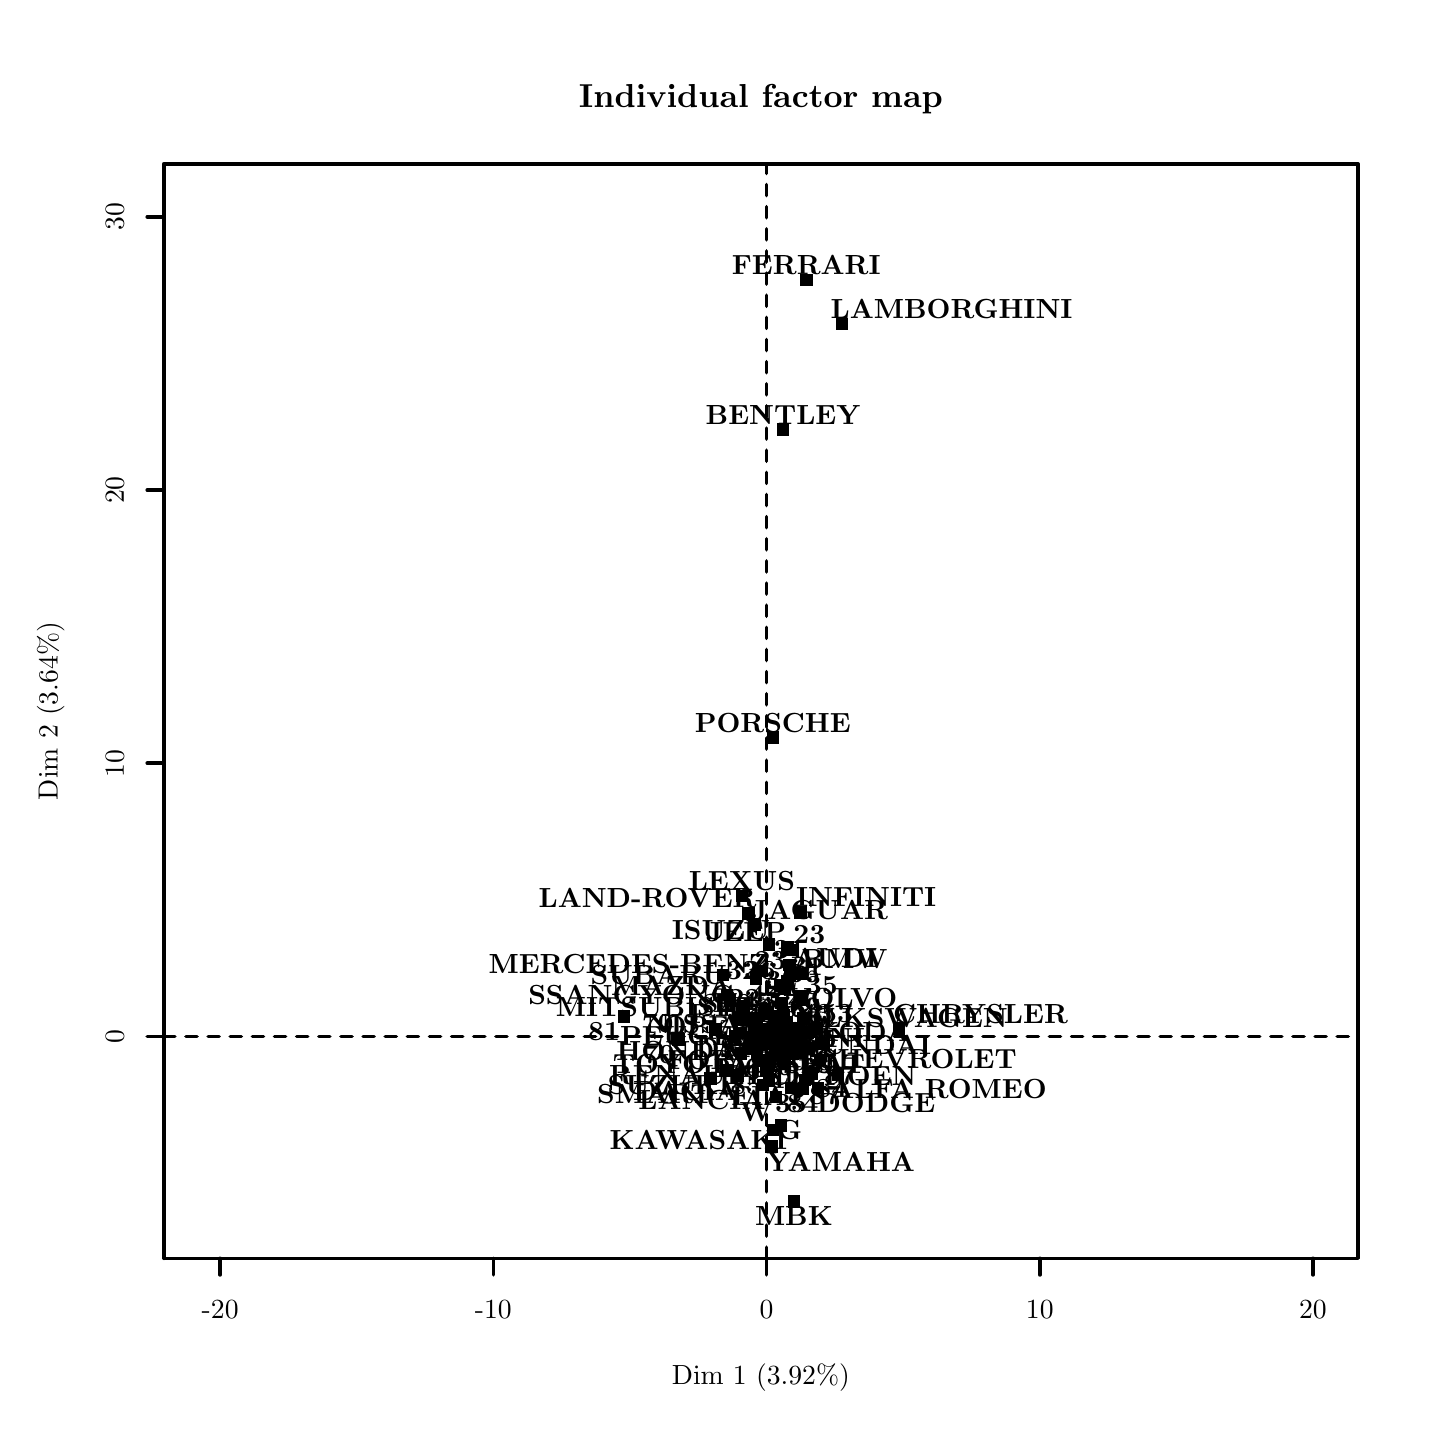
\begin{tikzpicture}[x=1pt,y=1pt]
\definecolor{fillColor}{RGB}{255,255,255}
\path[use as bounding box,fill=fillColor,fill opacity=0.00] (0,0) rectangle (505.89,505.89);
\begin{scope}
\path[clip] ( 49.20, 61.20) rectangle (480.69,456.69);
\definecolor{drawColor}{RGB}{255,255,255}

\path[draw=drawColor,line width= 1.3pt,line join=round,line cap=round] (267.00,141.35) circle (  2.25);
\end{scope}
\begin{scope}
\path[clip] (  0.00,  0.00) rectangle (505.89,505.89);
\definecolor{drawColor}{RGB}{0,0,0}

\path[draw=drawColor,line width= 1.3pt,line join=round,line cap=round] ( 69.55, 61.20) -- (464.45, 61.20);

\path[draw=drawColor,line width= 1.3pt,line join=round,line cap=round] ( 69.55, 61.20) -- ( 69.55, 55.20);

\path[draw=drawColor,line width= 1.3pt,line join=round,line cap=round] (168.28, 61.20) -- (168.28, 55.20);

\path[draw=drawColor,line width= 1.3pt,line join=round,line cap=round] (267.00, 61.20) -- (267.00, 55.20);

\path[draw=drawColor,line width= 1.3pt,line join=round,line cap=round] (365.73, 61.20) -- (365.73, 55.20);

\path[draw=drawColor,line width= 1.3pt,line join=round,line cap=round] (464.45, 61.20) -- (464.45, 55.20);

\node[text=drawColor,anchor=base,inner sep=0pt, outer sep=0pt, scale=  1.00] at ( 69.55, 39.60) {-20};

\node[text=drawColor,anchor=base,inner sep=0pt, outer sep=0pt, scale=  1.00] at (168.28, 39.60) {-10};

\node[text=drawColor,anchor=base,inner sep=0pt, outer sep=0pt, scale=  1.00] at (267.00, 39.60) {0};

\node[text=drawColor,anchor=base,inner sep=0pt, outer sep=0pt, scale=  1.00] at (365.73, 39.60) {10};

\node[text=drawColor,anchor=base,inner sep=0pt, outer sep=0pt, scale=  1.00] at (464.45, 39.60) {20};

\path[draw=drawColor,line width= 1.3pt,line join=round,line cap=round] ( 49.20,141.35) -- ( 49.20,437.52);

\path[draw=drawColor,line width= 1.3pt,line join=round,line cap=round] ( 49.20,141.35) -- ( 43.20,141.35);

\path[draw=drawColor,line width= 1.3pt,line join=round,line cap=round] ( 49.20,240.07) -- ( 43.20,240.07);

\path[draw=drawColor,line width= 1.3pt,line join=round,line cap=round] ( 49.20,338.80) -- ( 43.20,338.80);

\path[draw=drawColor,line width= 1.3pt,line join=round,line cap=round] ( 49.20,437.52) -- ( 43.20,437.52);

\node[text=drawColor,rotate= 90.00,anchor=base,inner sep=0pt, outer sep=0pt, scale=  1.00] at ( 34.80,141.35) {0};

\node[text=drawColor,rotate= 90.00,anchor=base,inner sep=0pt, outer sep=0pt, scale=  1.00] at ( 34.80,240.07) {10};

\node[text=drawColor,rotate= 90.00,anchor=base,inner sep=0pt, outer sep=0pt, scale=  1.00] at ( 34.80,338.80) {20};

\node[text=drawColor,rotate= 90.00,anchor=base,inner sep=0pt, outer sep=0pt, scale=  1.00] at ( 34.80,437.52) {30};

\path[draw=drawColor,line width= 1.3pt,line join=round,line cap=round] ( 49.20, 61.20) --
	(480.69, 61.20) --
	(480.69,456.69) --
	( 49.20,456.69) --
	( 49.20, 61.20);
\end{scope}
\begin{scope}
\path[clip] (  0.00,  0.00) rectangle (505.89,505.89);
\definecolor{drawColor}{RGB}{0,0,0}

\node[text=drawColor,anchor=base,inner sep=0pt, outer sep=0pt, scale=  1.20] at (264.94,477.15) {\bfseries Individual factor map};

\node[text=drawColor,anchor=base,inner sep=0pt, outer sep=0pt, scale=  1.00] at (264.94, 15.60) {Dim 1 (3.92{\%})};

\node[text=drawColor,rotate= 90.00,anchor=base,inner sep=0pt, outer sep=0pt, scale=  1.00] at ( 10.80,258.94) {Dim 2 (3.64{\%})};
\end{scope}
\begin{scope}
\path[clip] ( 49.20, 61.20) rectangle (480.69,456.69);
\definecolor{drawColor}{RGB}{0,0,0}

\path[draw=drawColor,line width= 1.3pt,dash pattern=on 4pt off 4pt ,line join=round,line cap=round] (267.00, 61.20) -- (267.00,456.69);

\path[draw=drawColor,line width= 1.3pt,dash pattern=on 4pt off 4pt ,line join=round,line cap=round] ( 49.20,141.35) -- (480.69,141.35);

\node[text=drawColor,anchor=base,inner sep=0pt, outer sep=0pt, scale=  1.00] at (276.77,145.46) {\bfseries D};

\node[text=drawColor,anchor=base,inner sep=0pt, outer sep=0pt, scale=  1.00] at (252.20,126.41) {\bfseries E};

\node[text=drawColor,anchor=base,inner sep=0pt, outer sep=0pt, scale=  1.00] at (252.19,149.89) {\bfseries H};

\node[text=drawColor,anchor=base,inner sep=0pt, outer sep=0pt, scale=  1.00] at (263.19,110.59) {\bfseries W};

\node[text=drawColor,anchor=base,inner sep=0pt, outer sep=0pt, scale=  1.00] at (275.31,104.10) {\bfseries G};

\node[text=drawColor,anchor=base,inner sep=0pt, outer sep=0pt, scale=  1.00] at (227.66,142.90) {\bfseries 70};

\node[text=drawColor,anchor=base,inner sep=0pt, outer sep=0pt, scale=  1.00] at (267.79,146.48) {\bfseries 46};

\node[text=drawColor,anchor=base,inner sep=0pt, outer sep=0pt, scale=  1.00] at (270.68,127.20) {\bfseries 56};

\node[text=drawColor,anchor=base,inner sep=0pt, outer sep=0pt, scale=  1.00] at (281.69,163.57) {\bfseries 31};

\node[text=drawColor,anchor=base,inner sep=0pt, outer sep=0pt, scale=  1.00] at (285.05,128.90) {\bfseries 60};

\node[text=drawColor,anchor=base,inner sep=0pt, outer sep=0pt, scale=  1.00] at (287.37,128.84) {\bfseries 55};

\node[text=drawColor,anchor=base,inner sep=0pt, outer sep=0pt, scale=  1.00] at (280.44,160.77) {\bfseries 36};

\node[text=drawColor,anchor=base,inner sep=0pt, outer sep=0pt, scale=  1.00] at (249.43,149.97) {\bfseries 82};

\node[text=drawColor,anchor=base,inner sep=0pt, outer sep=0pt, scale=  1.00] at (267.33,128.27) {\bfseries 52};

\node[text=drawColor,anchor=base,inner sep=0pt, outer sep=0pt, scale=  1.00] at (284.11,141.33) {\bfseries 47};

\node[text=drawColor,anchor=base,inner sep=0pt, outer sep=0pt, scale=  1.00] at (272.31,155.67) {\bfseries 21};

\node[text=drawColor,anchor=base,inner sep=0pt, outer sep=0pt, scale=  1.00] at (273.18,150.10) {\bfseries 53};

\node[text=drawColor,anchor=base,inner sep=0pt, outer sep=0pt, scale=  1.00] at (269.28,142.80) {\bfseries 54};

\node[text=drawColor,anchor=base,inner sep=0pt, outer sep=0pt, scale=  1.00] at (282.48,174.87) {\bfseries 23};

\node[text=drawColor,anchor=base,inner sep=0pt, outer sep=0pt, scale=  1.00] at (272.15,124.05) {\bfseries 81};

\node[text=drawColor,anchor=base,inner sep=0pt, outer sep=0pt, scale=  1.00] at (270.25,133.83) {\bfseries 48};

\node[text=drawColor,anchor=base,inner sep=0pt, outer sep=0pt, scale=  1.00] at (274.09,135.78) {\bfseries 34};

\node[text=drawColor,anchor=base,inner sep=0pt, outer sep=0pt, scale=  1.00] at (285.21,136.19) {\bfseries 64};

\node[text=drawColor,anchor=base,inner sep=0pt, outer sep=0pt, scale=  1.00] at (273.60,122.67) {\bfseries 42};

\node[text=drawColor,anchor=base,inner sep=0pt, outer sep=0pt, scale=  1.00] at (258.09,161.77) {\bfseries 32};

\node[text=drawColor,anchor=base,inner sep=0pt, outer sep=0pt, scale=  1.00] at (256.43,135.71) {\bfseries 43};

\node[text=drawColor,anchor=base,inner sep=0pt, outer sep=0pt, scale=  1.00] at (263.68,150.74) {\bfseries 45};

\node[text=drawColor,anchor=base,inner sep=0pt, outer sep=0pt, scale=  1.00] at (280.98,148.55) {\bfseries 69};

\node[text=drawColor,anchor=base,inner sep=0pt, outer sep=0pt, scale=  1.00] at (259.05,151.90) {\bfseries 22};

\node[text=drawColor,anchor=base,inner sep=0pt, outer sep=0pt, scale=  1.00] at (275.80,114.03) {\bfseries 35};

\node[text=drawColor,anchor=base,inner sep=0pt, outer sep=0pt, scale=  1.00] at (290.39,119.35) {\bfseries 84};

\node[text=drawColor,anchor=base,inner sep=0pt, outer sep=0pt, scale=  1.00] at (255.34,148.46) {\bfseries 10};

\node[text=drawColor,anchor=base,inner sep=0pt, outer sep=0pt, scale=  1.00] at (288.07,116.89) {\bfseries 87};

\node[text=drawColor,anchor=base,inner sep=0pt, outer sep=0pt, scale=  1.00] at (259.55,120.44) {\bfseries 85};

\node[text=drawColor,anchor=base,inner sep=0pt, outer sep=0pt, scale=  1.00] at (228.09,131.63) {\bfseries 70};

\node[text=drawColor,anchor=base,inner sep=0pt, outer sep=0pt, scale=  1.00] at (281.46,148.36) {\bfseries 54};

\node[text=drawColor,anchor=base,inner sep=0pt, outer sep=0pt, scale=  1.00] at (272.45,158.25) {\bfseries 32};

\node[text=drawColor,anchor=base,inner sep=0pt, outer sep=0pt, scale=  1.00] at (273.94,139.83) {\bfseries 56};

\node[text=drawColor,anchor=base,inner sep=0pt, outer sep=0pt, scale=  1.00] at (266.22,136.98) {\bfseries 52};

\node[text=drawColor,anchor=base,inner sep=0pt, outer sep=0pt, scale=  1.00] at (292.46,146.39) {\bfseries 53};

\node[text=drawColor,anchor=base,inner sep=0pt, outer sep=0pt, scale=  1.00] at (275.79,129.06) {\bfseries 60};

\node[text=drawColor,anchor=base,inner sep=0pt, outer sep=0pt, scale=  1.00] at (208.31,139.92) {\bfseries 81};

\node[text=drawColor,anchor=base,inner sep=0pt, outer sep=0pt, scale=  1.00] at (275.25,169.45) {\bfseries 31};

\node[text=drawColor,anchor=base,inner sep=0pt, outer sep=0pt, scale=  1.00] at (266.41,153.21) {\bfseries 45};

\node[text=drawColor,anchor=base,inner sep=0pt, outer sep=0pt, scale=  1.00] at (269.96,145.57) {\bfseries 47};

\node[text=drawColor,anchor=base,inner sep=0pt, outer sep=0pt, scale=  1.00] at (284.90,141.14) {\bfseries 64};

\node[text=drawColor,anchor=base,inner sep=0pt, outer sep=0pt, scale=  1.00] at (286.66,137.35) {\bfseries 55};

\node[text=drawColor,anchor=base,inner sep=0pt, outer sep=0pt, scale=  1.00] at (272.57,132.10) {\bfseries 48};

\node[text=drawColor,anchor=base,inner sep=0pt, outer sep=0pt, scale=  1.00] at (268.39,165.50) {\bfseries 23};

\node[text=drawColor,anchor=base,inner sep=0pt, outer sep=0pt, scale=  1.00] at (284.99,146.51) {\bfseries 43};

\node[text=drawColor,anchor=base,inner sep=0pt, outer sep=0pt, scale=  1.00] at (265.54,126.64) {\bfseries 42};

\node[text=drawColor,anchor=base,inner sep=0pt, outer sep=0pt, scale=  1.00] at (261.86,144.86) {\bfseries 21};

\node[text=drawColor,anchor=base,inner sep=0pt, outer sep=0pt, scale=  1.00] at (265.11,148.39) {\bfseries 22};

\node[text=drawColor,anchor=base,inner sep=0pt, outer sep=0pt, scale=  1.00] at (293.52,124.10) {\bfseries 87};

\node[text=drawColor,anchor=base,inner sep=0pt, outer sep=0pt, scale=  1.00] at (264.62,162.03) {\bfseries 36};

\node[text=drawColor,anchor=base,inner sep=0pt, outer sep=0pt, scale=  1.00] at (280.05,113.71) {\bfseries 84};

\node[text=drawColor,anchor=base,inner sep=0pt, outer sep=0pt, scale=  1.00] at (280.34,151.06) {\bfseries 46};

\node[text=drawColor,anchor=base,inner sep=0pt, outer sep=0pt, scale=  1.00] at (270.19,131.46) {\bfseries 34};

\node[text=drawColor,anchor=base,inner sep=0pt, outer sep=0pt, scale=  1.00] at (255.98,150.09) {\bfseries 10};

\node[text=drawColor,anchor=base,inner sep=0pt, outer sep=0pt, scale=  1.00] at (264.88,127.07) {\bfseries 69};

\node[text=drawColor,anchor=base,inner sep=0pt, outer sep=0pt, scale=  1.00] at (286.96,156.68) {\bfseries 35};

\node[text=drawColor,anchor=base,inner sep=0pt, outer sep=0pt, scale=  1.00] at (257.01,137.67) {\bfseries 2};

\node[text=drawColor,anchor=base,inner sep=0pt, outer sep=0pt, scale=  1.00] at (263.86,131.07) {\bfseries 5};

\node[text=drawColor,anchor=base,inner sep=0pt, outer sep=0pt, scale=  1.00] at (263.10,145.41) {\bfseries 1};

\node[text=drawColor,anchor=base,inner sep=0pt, outer sep=0pt, scale=  1.00] at (269.36,140.84) {\bfseries 3};

\node[text=drawColor,anchor=base,inner sep=0pt, outer sep=0pt, scale=  1.00] at (262.24,137.37) {\bfseries 4};

\node[text=drawColor,anchor=base,inner sep=0pt, outer sep=0pt, scale=  1.00] at (286.77,134.03) {\bfseries 6};

\node[text=drawColor,anchor=base,inner sep=0pt, outer sep=0pt, scale=  1.00] at (242.94,145.87) {\bfseries P};

\node[text=drawColor,anchor=base,inner sep=0pt, outer sep=0pt, scale=  1.00] at (287.49,144.76) {\bfseries C};

\node[text=drawColor,anchor=base,inner sep=0pt, outer sep=0pt, scale=  1.00] at (282.84,126.61) {\bfseries L};

\node[text=drawColor,anchor=base,inner sep=0pt, outer sep=0pt, scale=  1.00] at (282.06,126.32) {\bfseries F};

\node[text=drawColor,anchor=base,inner sep=0pt, outer sep=0pt, scale=  1.00] at (271.36,141.45) {\bfseries E};

\node[text=drawColor,anchor=base,inner sep=0pt, outer sep=0pt, scale=  1.00] at (257.64,126.37) {\bfseries A};

\node[text=drawColor,anchor=base,inner sep=0pt, outer sep=0pt, scale=  1.00] at (234.67,132.55) {\bfseries HONDA};

\node[text=drawColor,anchor=base,inner sep=0pt, outer sep=0pt, scale=  1.00] at (255.83,140.38) {\bfseries KIA};

\node[text=drawColor,anchor=base,inner sep=0pt, outer sep=0pt, scale=  1.00] at (294.40,151.94) {\bfseries VOLVO};

\node[text=drawColor,anchor=base,inner sep=0pt, outer sep=0pt, scale=  1.00] at (295.18,165.92) {\bfseries BMW};

\node[text=drawColor,anchor=base,inner sep=0pt, outer sep=0pt, scale=  1.00] at (236.20,128.01) {\bfseries TOYOTA};

\node[text=drawColor,anchor=base,inner sep=0pt, outer sep=0pt, scale=  1.00] at (217.06,164.27) {\bfseries MERCEDES-BENZ};

\node[text=drawColor,anchor=base,inner sep=0pt, outer sep=0pt, scale=  1.00] at (232.74,156.34) {\bfseries MAZDA};

\node[text=drawColor,anchor=base,inner sep=0pt, outer sep=0pt, scale=  1.00] at (294.09,123.82) {\bfseries CITROEN};

\node[text=drawColor,anchor=base,inner sep=0pt, outer sep=0pt, scale=  1.00] at (238.26,124.04) {\bfseries RENAULT};

\node[text=drawColor,anchor=base,inner sep=0pt, outer sep=0pt, scale=  1.00] at (242.82,137.98) {\bfseries PEUGEOT};

\node[text=drawColor,anchor=base,inner sep=0pt, outer sep=0pt, scale=  1.00] at (288.24,137.32) {\bfseries MINI};

\node[text=drawColor,anchor=base,inner sep=0pt, outer sep=0pt, scale=  1.00] at (242.39,100.36) {\bfseries KAWASAKI};

\node[text=drawColor,anchor=base,inner sep=0pt, outer sep=0pt, scale=  1.00] at (329.17,119.09) {\bfseries ALFA ROMEO};

\node[text=drawColor,anchor=base,inner sep=0pt, outer sep=0pt, scale=  1.00] at (269.24,251.30) {\bfseries PORSCHE};

\node[text=drawColor,anchor=base,inner sep=0pt, outer sep=0pt, scale=  1.00] at (312.23,144.66) {\bfseries VOLKSWAGEN};

\node[text=drawColor,anchor=base,inner sep=0pt, outer sep=0pt, scale=  1.00] at (231.80,120.42) {\bfseries SUZUKI};

\node[text=drawColor,anchor=base,inner sep=0pt, outer sep=0pt, scale=  1.00] at (258.11,194.12) {\bfseries LEXUS};

\node[text=drawColor,anchor=base,inner sep=0pt, outer sep=0pt, scale=  1.00] at (245.23,142.41) {\bfseries NISSAN};

\node[text=drawColor,anchor=base,inner sep=0pt, outer sep=0pt, scale=  1.00] at (224.01,187.84) {\bfseries LAND-ROVER};

\node[text=drawColor,anchor=base,inner sep=0pt, outer sep=0pt, scale=  1.00] at (244.98,141.57) {\bfseries OPEL};

\node[text=drawColor,anchor=base,inner sep=0pt, outer sep=0pt, scale=  1.00] at (320.90,129.94) {\bfseries CHEVROLET};

\node[text=drawColor,anchor=base,inner sep=0pt, outer sep=0pt, scale=  1.00] at (291.82,166.18) {\bfseries AUDI};

\node[text=drawColor,anchor=base,inner sep=0pt, outer sep=0pt, scale=  1.00] at (247.73,129.44) {\bfseries FORD};

\node[text=drawColor,anchor=base,inner sep=0pt, outer sep=0pt, scale=  1.00] at (226.29,148.71) {\bfseries MITSUBISHI};

\node[text=drawColor,anchor=base,inner sep=0pt, outer sep=0pt, scale=  1.00] at (267.95,116.44) {\bfseries FIAT};

\node[text=drawColor,anchor=base,inner sep=0pt, outer sep=0pt, scale=  1.00] at (293.78, 92.70) {\bfseries YAMAHA};

\node[text=drawColor,anchor=base,inner sep=0pt, outer sep=0pt, scale=  1.00] at (302.99,188.20) {\bfseries INFINITI};

\node[text=drawColor,anchor=base,inner sep=0pt, outer sep=0pt, scale=  1.00] at (297.93,134.70) {\bfseries HYUNDAI};

\node[text=drawColor,anchor=base,inner sep=0pt, outer sep=0pt, scale=  1.00] at (287.75,127.96) {\bfseries SEAT};

\node[text=drawColor,anchor=base,inner sep=0pt, outer sep=0pt, scale=  1.00] at (286.14,183.78) {\bfseries JAGUAR};

\node[text=drawColor,anchor=base,inner sep=0pt, outer sep=0pt, scale=  1.00] at (259.60,175.66) {\bfseries JEEP};

\node[text=drawColor,anchor=base,inner sep=0pt, outer sep=0pt, scale=  1.00] at (298.35,139.51) {\bfseries SKODA};

\node[text=drawColor,anchor=base,inner sep=0pt, outer sep=0pt, scale=  1.00] at (237.94,118.31) {\bfseries DACIA};

\node[text=drawColor,anchor=base,inner sep=0pt, outer sep=0pt, scale=  1.00] at (248.89,133.82) {\bfseries DS};

\node[text=drawColor,anchor=base,inner sep=0pt, outer sep=0pt, scale=  1.00] at (228.04,160.10) {\bfseries SUBARU};

\node[text=drawColor,anchor=base,inner sep=0pt, outer sep=0pt, scale=  1.00] at (250.51,176.52) {\bfseries ISUZU};

\node[text=drawColor,anchor=base,inner sep=0pt, outer sep=0pt, scale=  1.00] at (243.67,114.86) {\bfseries LANCIA};

\node[text=drawColor,anchor=base,inner sep=0pt, outer sep=0pt, scale=  1.00] at (276.88, 72.93) {\bfseries MBK};

\node[text=drawColor,anchor=base,inner sep=0pt, outer sep=0pt, scale=  1.00] at (226.64,117.24) {\bfseries SMART};

\node[text=drawColor,anchor=base,inner sep=0pt, outer sep=0pt, scale=  1.00] at (218.35,152.90) {\bfseries SSANGYONG};

\node[text=drawColor,anchor=base,inner sep=0pt, outer sep=0pt, scale=  1.00] at (281.36,416.68) {\bfseries FERRARI};

\node[text=drawColor,anchor=base,inner sep=0pt, outer sep=0pt, scale=  1.00] at (344.31,146.14) {\bfseries CHRYSLER};

\node[text=drawColor,anchor=base,inner sep=0pt, outer sep=0pt, scale=  1.00] at (306.50,113.90) {\bfseries DODGE};

\node[text=drawColor,anchor=base,inner sep=0pt, outer sep=0pt, scale=  1.00] at (272.94,362.61) {\bfseries BENTLEY};

\node[text=drawColor,anchor=base,inner sep=0pt, outer sep=0pt, scale=  1.00] at (333.85,400.74) {\bfseries LAMBORGHINI};

\node[text=drawColor,anchor=base,inner sep=0pt, outer sep=0pt, scale=  1.00] at (255.89,133.81) {\bfseries M};

\node[text=drawColor,anchor=base,inner sep=0pt, outer sep=0pt, scale=  1.00] at (287.77,127.93) {\bfseries U};
\definecolor{fillColor}{RGB}{0,0,0}

\path[fill=fillColor] (268.54,141.24) --
	(273.04,141.24) --
	(273.04,145.74) --
	(268.54,145.74) --
	cycle;

\path[fill=fillColor] (255.51,133.03) --
	(260.01,133.03) --
	(260.01,137.53) --
	(255.51,137.53) --
	cycle;

\path[fill=fillColor] (255.85,145.67) --
	(260.35,145.67) --
	(260.35,150.17) --
	(255.85,150.17) --
	cycle;

\path[fill=fillColor] (268.23,117.21) --
	(272.73,117.21) --
	(272.73,121.71) --
	(268.23,121.71) --
	cycle;

\path[fill=fillColor] (266.98,105.30) --
	(271.48,105.30) --
	(271.48,109.80) --
	(266.98,109.80) --
	cycle;

\path[fill=fillColor] (232.57,138.47) --
	(237.07,138.47) --
	(237.07,142.97) --
	(232.57,142.97) --
	cycle;

\path[fill=fillColor] (272.70,142.05) --
	(277.20,142.05) --
	(277.20,146.55) --
	(272.70,146.55) --
	cycle;

\path[fill=fillColor] (275.58,133.61) --
	(280.08,133.61) --
	(280.08,138.11) --
	(275.58,138.11) --
	cycle;

\path[fill=fillColor] (272.29,159.14) --
	(276.79,159.14) --
	(276.79,163.64) --
	(272.29,163.64) --
	cycle;

\path[fill=fillColor] (275.64,135.32) --
	(280.14,135.32) --
	(280.14,139.82) --
	(275.64,139.82) --
	cycle;

\path[fill=fillColor] (277.97,135.25) --
	(282.47,135.25) --
	(282.47,139.75) --
	(277.97,139.75) --
	cycle;

\path[fill=fillColor] (271.03,156.34) --
	(275.53,156.34) --
	(275.53,160.84) --
	(271.03,160.84) --
	cycle;

\path[fill=fillColor] (254.34,145.55) --
	(258.84,145.55) --
	(258.84,150.05) --
	(254.34,150.05) --
	cycle;

\path[fill=fillColor] (272.23,134.68) --
	(276.73,134.68) --
	(276.73,139.18) --
	(272.23,139.18) --
	cycle;

\path[fill=fillColor] (274.71,136.90) --
	(279.21,136.90) --
	(279.21,141.40) --
	(274.71,141.40) --
	cycle;

\path[fill=fillColor] (270.06,151.24) --
	(274.56,151.24) --
	(274.56,155.74) --
	(270.06,155.74) --
	cycle;

\path[fill=fillColor] (278.08,145.67) --
	(282.58,145.67) --
	(282.58,150.17) --
	(278.08,150.17) --
	cycle;

\path[fill=fillColor] (274.18,138.37) --
	(278.68,138.37) --
	(278.68,142.87) --
	(274.18,142.87) --
	cycle;

\path[fill=fillColor] (273.08,170.44) --
	(277.58,170.44) --
	(277.58,174.94) --
	(273.08,174.94) --
	cycle;

\path[fill=fillColor] (262.74,130.46) --
	(267.24,130.46) --
	(267.24,134.96) --
	(262.74,134.96) --
	cycle;

\path[fill=fillColor] (275.15,140.24) --
	(279.65,140.24) --
	(279.65,144.74) --
	(275.15,144.74) --
	cycle;

\path[fill=fillColor] (271.84,142.20) --
	(276.34,142.20) --
	(276.34,146.70) --
	(271.84,146.70) --
	cycle;

\path[fill=fillColor] (275.80,137.18) --
	(280.30,137.18) --
	(280.30,141.68) --
	(275.80,141.68) --
	cycle;

\path[fill=fillColor] (271.35,129.08) --
	(275.85,129.08) --
	(275.85,133.58) --
	(271.35,133.58) --
	cycle;

\path[fill=fillColor] (263.00,162.76) --
	(267.50,162.76) --
	(267.50,167.26) --
	(263.00,167.26) --
	cycle;

\path[fill=fillColor] (261.34,142.12) --
	(265.84,142.12) --
	(265.84,146.62) --
	(261.34,146.62) --
	cycle;

\path[fill=fillColor] (268.59,146.31) --
	(273.09,146.31) --
	(273.09,150.81) --
	(268.59,150.81) --
	cycle;

\path[fill=fillColor] (271.58,144.12) --
	(276.08,144.12) --
	(276.08,148.62) --
	(271.58,148.62) --
	cycle;

\path[fill=fillColor] (263.96,147.47) --
	(268.46,147.47) --
	(268.46,151.97) --
	(263.96,151.97) --
	cycle;

\path[fill=fillColor] (273.55,120.45) --
	(278.05,120.45) --
	(278.05,124.95) --
	(273.55,124.95) --
	cycle;

\path[fill=fillColor] (280.99,125.77) --
	(285.49,125.77) --
	(285.49,130.27) --
	(280.99,130.27) --
	cycle;

\path[fill=fillColor] (260.24,144.03) --
	(264.74,144.03) --
	(264.74,148.53) --
	(260.24,148.53) --
	cycle;

\path[fill=fillColor] (278.67,123.31) --
	(283.17,123.31) --
	(283.17,127.81) --
	(278.67,127.81) --
	cycle;

\path[fill=fillColor] (264.46,126.85) --
	(268.96,126.85) --
	(268.96,131.35) --
	(264.46,131.35) --
	cycle;

\path[fill=fillColor] (233.00,138.05) --
	(237.50,138.05) --
	(237.50,142.55) --
	(233.00,142.55) --
	cycle;

\path[fill=fillColor] (272.05,143.93) --
	(276.55,143.93) --
	(276.55,148.43) --
	(272.05,148.43) --
	cycle;

\path[fill=fillColor] (277.36,153.83) --
	(281.86,153.83) --
	(281.86,158.33) --
	(277.36,158.33) --
	cycle;

\path[fill=fillColor] (271.69,135.40) --
	(276.19,135.40) --
	(276.19,139.90) --
	(271.69,139.90) --
	cycle;

\path[fill=fillColor] (271.12,137.97) --
	(275.62,137.97) --
	(275.62,142.47) --
	(271.12,142.47) --
	cycle;

\path[fill=fillColor] (283.06,141.96) --
	(287.56,141.96) --
	(287.56,146.46) --
	(283.06,146.46) --
	cycle;

\path[fill=fillColor] (273.54,135.48) --
	(278.04,135.48) --
	(278.04,139.98) --
	(273.54,139.98) --
	cycle;

\path[fill=fillColor] (213.22,146.33) --
	(217.72,146.33) --
	(217.72,150.83) --
	(213.22,150.83) --
	cycle;

\path[fill=fillColor] (273.00,165.02) --
	(277.50,165.02) --
	(277.50,169.52) --
	(273.00,169.52) --
	cycle;

\path[fill=fillColor] (264.16,148.78) --
	(268.66,148.78) --
	(268.66,153.28) --
	(264.16,153.28) --
	cycle;

\path[fill=fillColor] (274.86,141.15) --
	(279.36,141.15) --
	(279.36,145.65) --
	(274.86,145.65) --
	cycle;

\path[fill=fillColor] (275.49,136.71) --
	(279.99,136.71) --
	(279.99,141.21) --
	(275.49,141.21) --
	cycle;

\path[fill=fillColor] (277.25,138.35) --
	(281.75,138.35) --
	(281.75,142.85) --
	(277.25,142.85) --
	cycle;

\path[fill=fillColor] (270.32,138.51) --
	(274.82,138.51) --
	(274.82,143.01) --
	(270.32,143.01) --
	cycle;

\path[fill=fillColor] (273.30,161.07) --
	(277.80,161.07) --
	(277.80,165.57) --
	(273.30,165.57) --
	cycle;

\path[fill=fillColor] (275.58,142.08) --
	(280.08,142.08) --
	(280.08,146.58) --
	(275.58,146.58) --
	cycle;

\path[fill=fillColor] (270.44,133.06) --
	(274.94,133.06) --
	(274.94,137.56) --
	(270.44,137.56) --
	cycle;

\path[fill=fillColor] (266.76,140.43) --
	(271.26,140.43) --
	(271.26,144.93) --
	(266.76,144.93) --
	cycle;

\path[fill=fillColor] (270.02,143.96) --
	(274.52,143.96) --
	(274.52,148.46) --
	(270.02,148.46) --
	cycle;

\path[fill=fillColor] (284.11,130.51) --
	(288.61,130.51) --
	(288.61,135.01) --
	(284.11,135.01) --
	cycle;

\path[fill=fillColor] (269.53,157.60) --
	(274.03,157.60) --
	(274.03,162.10) --
	(269.53,162.10) --
	cycle;

\path[fill=fillColor] (277.80,120.12) --
	(282.30,120.12) --
	(282.30,124.62) --
	(277.80,124.62) --
	cycle;

\path[fill=fillColor] (270.94,146.63) --
	(275.44,146.63) --
	(275.44,151.13) --
	(270.94,151.13) --
	cycle;

\path[fill=fillColor] (267.94,137.87) --
	(272.44,137.87) --
	(272.44,142.37) --
	(267.94,142.37) --
	cycle;

\path[fill=fillColor] (260.89,145.66) --
	(265.39,145.66) --
	(265.39,150.16) --
	(260.89,150.16) --
	cycle;

\path[fill=fillColor] (269.78,133.48) --
	(274.28,133.48) --
	(274.28,137.98) --
	(269.78,137.98) --
	cycle;

\path[fill=fillColor] (277.55,152.25) --
	(282.05,152.25) --
	(282.05,156.75) --
	(277.55,156.75) --
	cycle;

\path[fill=fillColor] (259.42,138.66) --
	(263.92,138.66) --
	(263.92,143.16) --
	(259.42,143.16) --
	cycle;

\path[fill=fillColor] (266.26,137.48) --
	(270.76,137.48) --
	(270.76,141.98) --
	(266.26,141.98) --
	cycle;

\path[fill=fillColor] (265.50,140.98) --
	(270.00,140.98) --
	(270.00,145.48) --
	(265.50,145.48) --
	cycle;

\path[fill=fillColor] (267.11,136.41) --
	(271.61,136.41) --
	(271.61,140.91) --
	(267.11,140.91) --
	cycle;

\path[fill=fillColor] (264.65,138.36) --
	(269.15,138.36) --
	(269.15,142.86) --
	(264.65,142.86) --
	cycle;

\path[fill=fillColor] (279.86,135.02) --
	(284.36,135.02) --
	(284.36,139.52) --
	(279.86,139.52) --
	cycle;

\path[fill=fillColor] (246.25,141.64) --
	(250.75,141.64) --
	(250.75,146.14) --
	(246.25,146.14) --
	cycle;

\path[fill=fillColor] (279.47,140.54) --
	(283.97,140.54) --
	(283.97,145.04) --
	(279.47,145.04) --
	cycle;

\path[fill=fillColor] (275.31,133.23) --
	(279.81,133.23) --
	(279.81,137.73) --
	(275.31,137.73) --
	cycle;

\path[fill=fillColor] (274.39,132.94) --
	(278.89,132.94) --
	(278.89,137.44) --
	(274.39,137.44) --
	cycle;

\path[fill=fillColor] (274.67,137.23) --
	(279.17,137.23) --
	(279.17,141.73) --
	(274.67,141.73) --
	cycle;

\path[fill=fillColor] (261.30,132.99) --
	(265.80,132.99) --
	(265.80,137.49) --
	(261.30,137.49) --
	cycle;

\path[fill=fillColor] (253.39,139.17) --
	(257.89,139.17) --
	(257.89,143.67) --
	(253.39,143.67) --
	cycle;

\path[fill=fillColor] (265.18,141.58) --
	(269.68,141.58) --
	(269.68,146.08) --
	(265.18,146.08) --
	cycle;

\path[fill=fillColor] (272.43,158.56) --
	(276.93,158.56) --
	(276.93,163.06) --
	(272.43,163.06) --
	cycle;

\path[fill=fillColor] (277.51,161.70) --
	(282.01,161.70) --
	(282.01,166.20) --
	(277.51,166.20) --
	cycle;

\path[fill=fillColor] (258.05,134.63) --
	(262.55,134.63) --
	(262.55,139.13) --
	(258.05,139.13) --
	cycle;

\path[fill=fillColor] (260.91,160.04) --
	(265.41,160.04) --
	(265.41,164.54) --
	(260.91,164.54) --
	cycle;

\path[fill=fillColor] (251.47,152.12) --
	(255.97,152.12) --
	(255.97,156.62) --
	(251.47,156.62) --
	cycle;

\path[fill=fillColor] (266.07,130.44) --
	(270.57,130.44) --
	(270.57,134.94) --
	(266.07,134.94) --
	cycle;

\path[fill=fillColor] (262.68,130.66) --
	(267.18,130.66) --
	(267.18,135.16) --
	(262.68,135.16) --
	cycle;

\path[fill=fillColor] (268.10,133.76) --
	(272.60,133.76) --
	(272.60,138.26) --
	(268.10,138.26) --
	cycle;

\path[fill=fillColor] (271.89,138.52) --
	(276.39,138.52) --
	(276.39,143.02) --
	(271.89,143.02) --
	cycle;

\path[fill=fillColor] (269.93,106.98) --
	(274.43,106.98) --
	(274.43,111.48) --
	(269.93,111.48) --
	cycle;

\path[fill=fillColor] (290.47,125.22) --
	(294.97,125.22) --
	(294.97,129.72) --
	(290.47,129.72) --
	cycle;

\path[fill=fillColor] (266.99,247.08) --
	(271.49,247.08) --
	(271.49,251.58) --
	(266.99,251.58) --
	cycle;

\path[fill=fillColor] (271.27,140.44) --
	(275.77,140.44) --
	(275.77,144.94) --
	(271.27,144.94) --
	cycle;

\path[fill=fillColor] (250.73,127.05) --
	(255.23,127.05) --
	(255.23,131.55) --
	(250.73,131.55) --
	cycle;

\path[fill=fillColor] (255.86,189.90) --
	(260.36,189.90) --
	(260.36,194.40) --
	(255.86,194.40) --
	cycle;

\path[fill=fillColor] (263.75,138.18) --
	(268.25,138.18) --
	(268.25,142.68) --
	(263.75,142.68) --
	cycle;

\path[fill=fillColor] (258.15,183.62) --
	(262.65,183.62) --
	(262.65,188.12) --
	(258.15,188.12) --
	cycle;

\path[fill=fillColor] (258.70,137.35) --
	(263.20,137.35) --
	(263.20,141.85) --
	(258.70,141.85) --
	cycle;

\path[fill=fillColor] (284.42,136.56) --
	(288.92,136.56) --
	(288.92,141.06) --
	(284.42,141.06) --
	cycle;

\path[fill=fillColor] (274.43,161.96) --
	(278.93,161.96) --
	(278.93,166.46) --
	(274.43,166.46) --
	cycle;

\path[fill=fillColor] (262.15,136.06) --
	(266.65,136.06) --
	(266.65,140.56) --
	(262.15,140.56) --
	cycle;

\path[fill=fillColor] (256.40,149.91) --
	(260.90,149.91) --
	(260.90,154.41) --
	(256.40,154.41) --
	cycle;

\path[fill=fillColor] (265.70,123.06) --
	(270.20,123.06) --
	(270.20,127.56) --
	(265.70,127.56) --
	cycle;

\path[fill=fillColor] (266.46, 99.32) --
	(270.96, 99.32) --
	(270.96,103.82) --
	(266.46,103.82) --
	cycle;

\path[fill=fillColor] (276.99,183.98) --
	(281.49,183.98) --
	(281.49,188.48) --
	(276.99,188.48) --
	cycle;

\path[fill=fillColor] (269.29,141.32) --
	(273.79,141.32) --
	(273.79,145.82) --
	(269.29,145.82) --
	cycle;

\path[fill=fillColor] (270.22,134.58) --
	(274.72,134.58) --
	(274.72,139.08) --
	(270.22,139.08) --
	cycle;

\path[fill=fillColor] (260.45,179.56) --
	(264.95,179.56) --
	(264.95,184.06) --
	(260.45,184.06) --
	cycle;

\path[fill=fillColor] (272.28,171.44) --
	(276.78,171.44) --
	(276.78,175.94) --
	(272.28,175.94) --
	cycle;

\path[fill=fillColor] (275.97,135.29) --
	(280.47,135.29) --
	(280.47,139.79) --
	(275.97,139.79) --
	cycle;

\path[fill=fillColor] (254.30,124.93) --
	(258.80,124.93) --
	(258.80,129.43) --
	(254.30,129.43) --
	cycle;

\path[fill=fillColor] (255.40,140.44) --
	(259.90,140.44) --
	(259.90,144.94) --
	(255.40,144.94) --
	cycle;

\path[fill=fillColor] (249.06,161.30) --
	(253.56,161.30) --
	(253.56,165.80) --
	(249.06,165.80) --
	cycle;

\path[fill=fillColor] (265.55,172.30) --
	(270.05,172.30) --
	(270.05,176.80) --
	(265.55,176.80) --
	cycle;

\path[fill=fillColor] (263.37,121.49) --
	(267.87,121.49) --
	(267.87,125.99) --
	(263.37,125.99) --
	cycle;

\path[fill=fillColor] (274.63, 79.55) --
	(279.13, 79.55) --
	(279.13, 84.05) --
	(274.63, 84.05) --
	cycle;

\path[fill=fillColor] (244.53,123.86) --
	(249.03,123.86) --
	(249.03,128.36) --
	(244.53,128.36) --
	cycle;

\path[fill=fillColor] (250.54,154.10) --
	(255.04,154.10) --
	(255.04,158.60) --
	(250.54,158.60) --
	cycle;

\path[fill=fillColor] (279.11,412.46) --
	(283.61,412.46) --
	(283.61,416.96) --
	(279.11,416.96) --
	cycle;

\path[fill=fillColor] (312.55,141.92) --
	(317.05,141.92) --
	(317.05,146.42) --
	(312.55,146.42) --
	cycle;

\path[fill=fillColor] (283.24,120.53) --
	(287.74,120.53) --
	(287.74,125.03) --
	(283.24,125.03) --
	cycle;

\path[fill=fillColor] (270.69,358.39) --
	(275.19,358.39) --
	(275.19,362.89) --
	(270.69,362.89) --
	cycle;

\path[fill=fillColor] (291.99,396.52) --
	(296.49,396.52) --
	(296.49,401.02) --
	(291.99,401.02) --
	cycle;

\path[fill=fillColor] (260.38,140.43) --
	(264.88,140.43) --
	(264.88,144.93) --
	(260.38,144.93) --
	cycle;

\path[fill=fillColor] (279.62,134.55) --
	(284.12,134.55) --
	(284.12,139.05) --
	(279.62,139.05) --
	cycle;
\end{scope}
\end{tikzpicture}
}
\caption{\label{fig:famd1} Analogous of Figure~\ref{fig:mca1}, categorical features' levels involved in the \gls{famd} can be plotted but not much can be drawn from the graph.}
\end{subfigure}%
\columnbreak
\hspace*{1cm} \begin{subfigure}[t]{0.45\textwidth}
\centering
\resizebox{\textwidth}{!}{% Created by tikzDevice version 0.12 on 2019-03-01 10:36:22
% !TEX encoding = UTF-8 Unicode
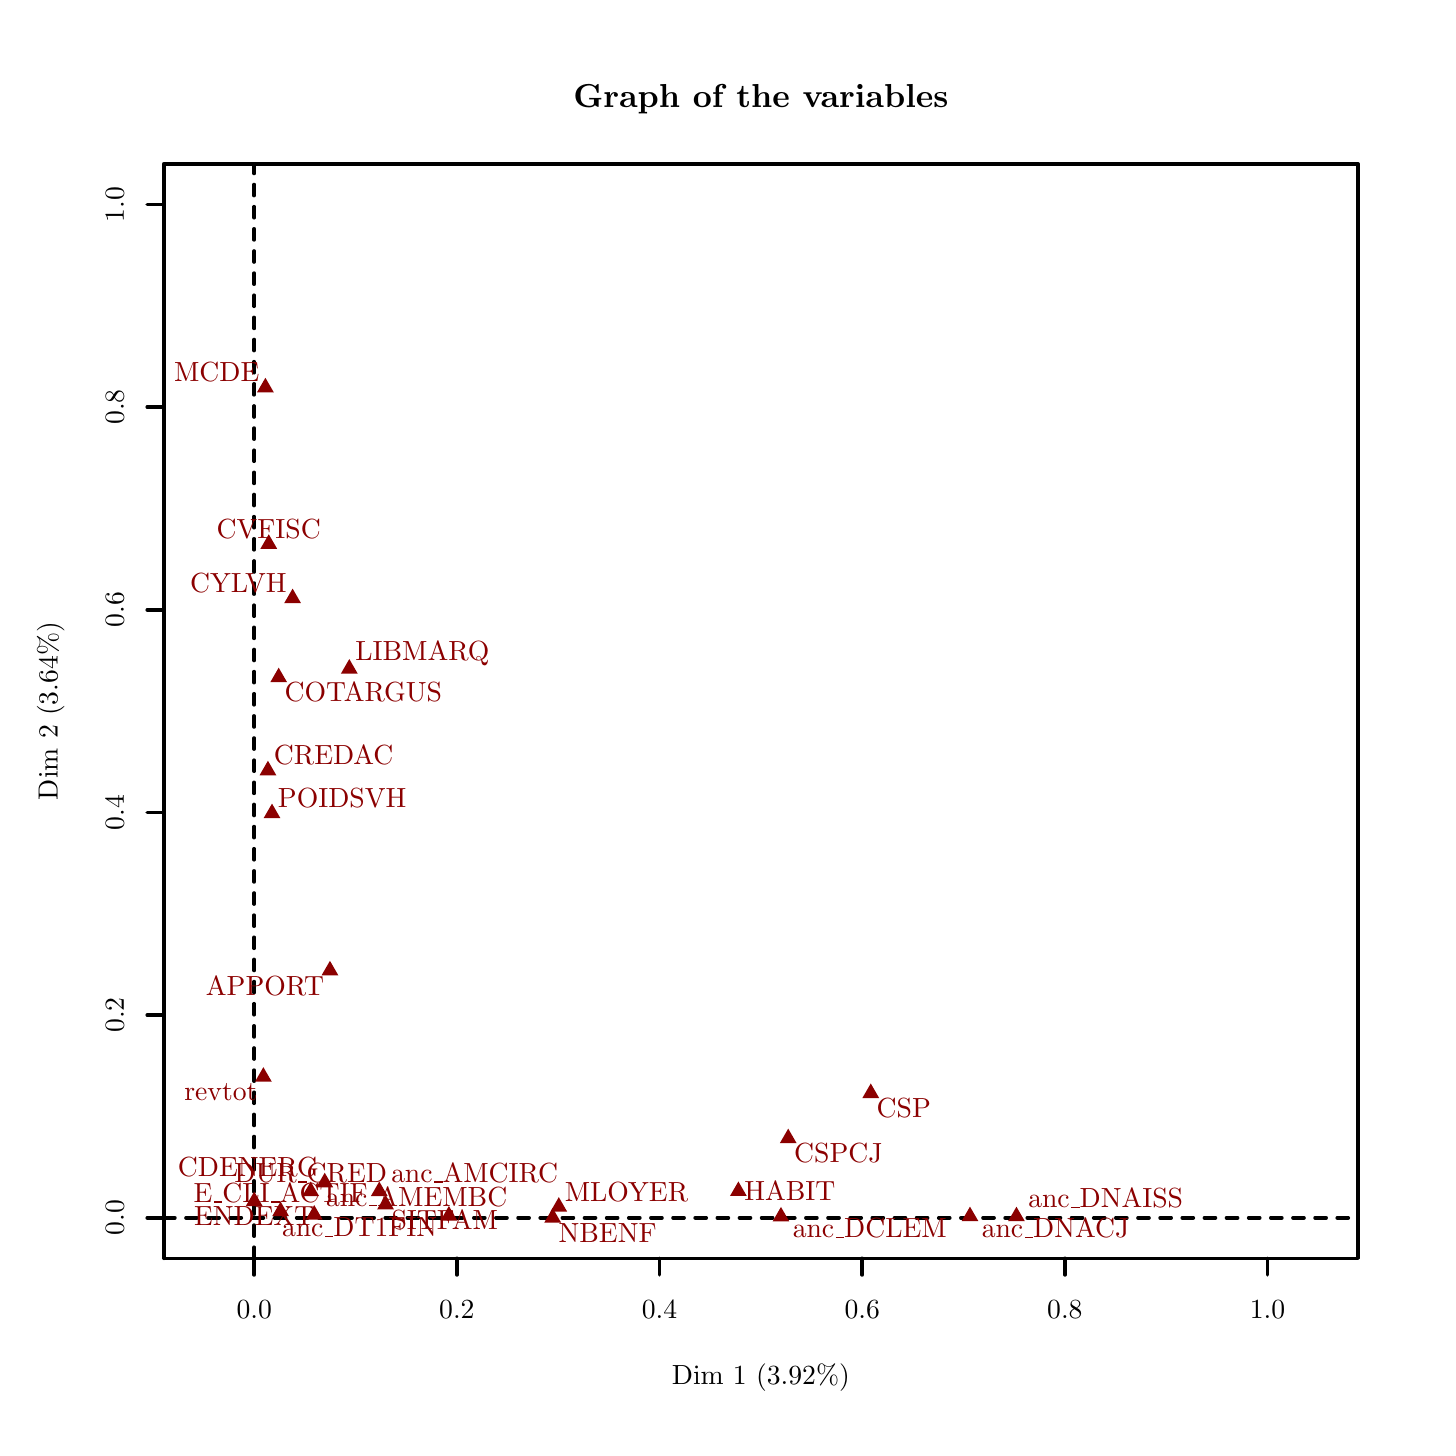
\begin{tikzpicture}[x=1pt,y=1pt]
\definecolor{fillColor}{RGB}{255,255,255}
\path[use as bounding box,fill=fillColor,fill opacity=0.00] (0,0) rectangle (505.89,505.89);
\begin{scope}
\path[clip] ( 49.20, 61.20) rectangle (480.69,456.69);
\definecolor{drawColor}{RGB}{255,255,255}

\path[draw=drawColor,line width= 1.3pt,line join=round,line cap=round] ( 81.85, 75.85) circle (  2.25);
\end{scope}
\begin{scope}
\path[clip] (  0.00,  0.00) rectangle (505.89,505.89);
\definecolor{drawColor}{RGB}{0,0,0}

\path[draw=drawColor,line width= 1.3pt,line join=round,line cap=round] ( 81.85, 61.20) -- (448.04, 61.20);

\path[draw=drawColor,line width= 1.3pt,line join=round,line cap=round] ( 81.85, 61.20) -- ( 81.85, 55.20);

\path[draw=drawColor,line width= 1.3pt,line join=round,line cap=round] (155.09, 61.20) -- (155.09, 55.20);

\path[draw=drawColor,line width= 1.3pt,line join=round,line cap=round] (228.33, 61.20) -- (228.33, 55.20);

\path[draw=drawColor,line width= 1.3pt,line join=round,line cap=round] (301.56, 61.20) -- (301.56, 55.20);

\path[draw=drawColor,line width= 1.3pt,line join=round,line cap=round] (374.80, 61.20) -- (374.80, 55.20);

\path[draw=drawColor,line width= 1.3pt,line join=round,line cap=round] (448.04, 61.20) -- (448.04, 55.20);

\node[text=drawColor,anchor=base,inner sep=0pt, outer sep=0pt, scale=  1.00] at ( 81.85, 39.60) {0.0};

\node[text=drawColor,anchor=base,inner sep=0pt, outer sep=0pt, scale=  1.00] at (155.09, 39.60) {0.2};

\node[text=drawColor,anchor=base,inner sep=0pt, outer sep=0pt, scale=  1.00] at (228.33, 39.60) {0.4};

\node[text=drawColor,anchor=base,inner sep=0pt, outer sep=0pt, scale=  1.00] at (301.56, 39.60) {0.6};

\node[text=drawColor,anchor=base,inner sep=0pt, outer sep=0pt, scale=  1.00] at (374.80, 39.60) {0.8};

\node[text=drawColor,anchor=base,inner sep=0pt, outer sep=0pt, scale=  1.00] at (448.04, 39.60) {1.0};

\path[draw=drawColor,line width= 1.3pt,line join=round,line cap=round] ( 49.20, 75.85) -- ( 49.20,442.04);

\path[draw=drawColor,line width= 1.3pt,line join=round,line cap=round] ( 49.20, 75.85) -- ( 43.20, 75.85);

\path[draw=drawColor,line width= 1.3pt,line join=round,line cap=round] ( 49.20,149.09) -- ( 43.20,149.09);

\path[draw=drawColor,line width= 1.3pt,line join=round,line cap=round] ( 49.20,222.33) -- ( 43.20,222.33);

\path[draw=drawColor,line width= 1.3pt,line join=round,line cap=round] ( 49.20,295.56) -- ( 43.20,295.56);

\path[draw=drawColor,line width= 1.3pt,line join=round,line cap=round] ( 49.20,368.80) -- ( 43.20,368.80);

\path[draw=drawColor,line width= 1.3pt,line join=round,line cap=round] ( 49.20,442.04) -- ( 43.20,442.04);

\node[text=drawColor,rotate= 90.00,anchor=base,inner sep=0pt, outer sep=0pt, scale=  1.00] at ( 34.80, 75.85) {0.0};

\node[text=drawColor,rotate= 90.00,anchor=base,inner sep=0pt, outer sep=0pt, scale=  1.00] at ( 34.80,149.09) {0.2};

\node[text=drawColor,rotate= 90.00,anchor=base,inner sep=0pt, outer sep=0pt, scale=  1.00] at ( 34.80,222.33) {0.4};

\node[text=drawColor,rotate= 90.00,anchor=base,inner sep=0pt, outer sep=0pt, scale=  1.00] at ( 34.80,295.56) {0.6};

\node[text=drawColor,rotate= 90.00,anchor=base,inner sep=0pt, outer sep=0pt, scale=  1.00] at ( 34.80,368.80) {0.8};

\node[text=drawColor,rotate= 90.00,anchor=base,inner sep=0pt, outer sep=0pt, scale=  1.00] at ( 34.80,442.04) {1.0};

\path[draw=drawColor,line width= 1.3pt,line join=round,line cap=round] ( 49.20, 61.20) --
	(480.69, 61.20) --
	(480.69,456.69) --
	( 49.20,456.69) --
	( 49.20, 61.20);
\end{scope}
\begin{scope}
\path[clip] (  0.00,  0.00) rectangle (505.89,505.89);
\definecolor{drawColor}{RGB}{0,0,0}

\node[text=drawColor,anchor=base,inner sep=0pt, outer sep=0pt, scale=  1.20] at (264.94,477.15) {\bfseries Graph of the variables};

\node[text=drawColor,anchor=base,inner sep=0pt, outer sep=0pt, scale=  1.00] at (264.94, 15.60) {Dim 1 (3.92{\%})};

\node[text=drawColor,rotate= 90.00,anchor=base,inner sep=0pt, outer sep=0pt, scale=  1.00] at ( 10.80,258.94) {Dim 2 (3.64{\%})};
\end{scope}
\begin{scope}
\path[clip] ( 49.20, 61.20) rectangle (480.69,456.69);
\definecolor{drawColor}{RGB}{0,0,0}

\path[draw=drawColor,line width= 1.3pt,dash pattern=on 4pt off 4pt ,line join=round,line cap=round] ( 81.85, 61.20) -- ( 81.85,456.69);

\path[draw=drawColor,line width= 1.3pt,dash pattern=on 4pt off 4pt ,line join=round,line cap=round] ( 49.20, 75.85) -- (480.69, 75.85);
\definecolor{drawColor}{RGB}{139,0,0}

\node[text=drawColor,anchor=base,inner sep=0pt, outer sep=0pt, scale=  1.00] at ( 85.75,156.32) {APPORT};

\node[text=drawColor,anchor=base,inner sep=0pt, outer sep=0pt, scale=  1.00] at (121.29,262.25) {COTARGUS};

\node[text=drawColor,anchor=base,inner sep=0pt, outer sep=0pt, scale=  1.00] at (110.57,239.47) {CREDAC};

\node[text=drawColor,anchor=base,inner sep=0pt, outer sep=0pt, scale=  1.00] at ( 87.12,321.31) {CVFISC};

\node[text=drawColor,anchor=base,inner sep=0pt, outer sep=0pt, scale=  1.00] at ( 76.14,301.66) {CYLVH};

\node[text=drawColor,anchor=base,inner sep=0pt, outer sep=0pt, scale=  1.00] at (102.27, 88.58) {DUR{\_{}}CRED};

\node[text=drawColor,anchor=base,inner sep=0pt, outer sep=0pt, scale=  1.00] at ( 81.86, 72.95) {ENDEXT};

\node[text=drawColor,anchor=base,inner sep=0pt, outer sep=0pt, scale=  1.00] at ( 68.33,377.86) {MCDE};

\node[text=drawColor,anchor=base,inner sep=0pt, outer sep=0pt, scale=  1.00] at (216.37, 81.78) {MLOYER};

\node[text=drawColor,anchor=base,inner sep=0pt, outer sep=0pt, scale=  1.00] at (209.57, 67.00) {NBENF};

\node[text=drawColor,anchor=base,inner sep=0pt, outer sep=0pt, scale=  1.00] at (113.63,223.98) {POIDSVH};

\node[text=drawColor,anchor=base,inner sep=0pt, outer sep=0pt, scale=  1.00] at (161.51, 88.59) {anc{\_{}}AMCIRC};

\node[text=drawColor,anchor=base,inner sep=0pt, outer sep=0pt, scale=  1.00] at (140.55, 80.09) {anc{\_{}}AMEMBC};

\node[text=drawColor,anchor=base,inner sep=0pt, outer sep=0pt, scale=  1.00] at (304.28, 68.56) {anc{\_{}}DCLEM};

\node[text=drawColor,anchor=base,inner sep=0pt, outer sep=0pt, scale=  1.00] at (389.51, 79.48) {anc{\_{}}DNAISS};

\node[text=drawColor,anchor=base,inner sep=0pt, outer sep=0pt, scale=  1.00] at (371.40, 68.68) {anc{\_{}}DNACJ};

\node[text=drawColor,anchor=base,inner sep=0pt, outer sep=0pt, scale=  1.00] at (119.92, 68.90) {anc{\_{}}DT1FIN};

\node[text=drawColor,anchor=base,inner sep=0pt, outer sep=0pt, scale=  1.00] at ( 69.81,118.27) {revtot};

\node[text=drawColor,anchor=base,inner sep=0pt, outer sep=0pt, scale=  1.00] at ( 79.73, 90.59) {CDENERG};

\node[text=drawColor,anchor=base,inner sep=0pt, outer sep=0pt, scale=  1.00] at (316.60,112.00) {CSP};

\node[text=drawColor,anchor=base,inner sep=0pt, outer sep=0pt, scale=  1.00] at (292.95, 95.68) {CSPCJ};

\node[text=drawColor,anchor=base,inner sep=0pt, outer sep=0pt, scale=  1.00] at ( 91.40, 81.33) {E{\_{}}CLI{\_{}}ACTIF};

\node[text=drawColor,anchor=base,inner sep=0pt, outer sep=0pt, scale=  1.00] at (275.42, 82.02) {HABIT};

\node[text=drawColor,anchor=base,inner sep=0pt, outer sep=0pt, scale=  1.00] at (142.61,277.19) {LIBMARQ};

\node[text=drawColor,anchor=base,inner sep=0pt, outer sep=0pt, scale=  1.00] at (150.71, 71.77) {SITFAM};
\definecolor{fillColor}{RGB}{139,0,0}

\path[fill=fillColor] (109.23,168.69) --
	(112.26,163.44) --
	(106.19,163.44) --
	cycle;

\path[fill=fillColor] ( 90.70,274.62) --
	( 93.73,269.37) --
	( 87.67,269.37) --
	cycle;

\path[fill=fillColor] ( 86.82,240.99) --
	( 89.85,235.74) --
	( 83.79,235.74) --
	cycle;

\path[fill=fillColor] ( 87.12,322.83) --
	( 90.15,317.58) --
	( 84.09,317.58) --
	cycle;

\path[fill=fillColor] ( 95.73,303.19) --
	( 98.76,297.94) --
	( 92.70,297.94) --
	cycle;

\path[fill=fillColor] (102.27, 88.94) --
	(105.30, 83.69) --
	( 99.24, 83.69) --
	cycle;

\path[fill=fillColor] ( 81.86, 85.31) --
	( 84.89, 80.07) --
	( 78.83, 80.07) --
	cycle;

\path[fill=fillColor] ( 85.90,379.38) --
	( 88.93,374.13) --
	( 82.87,374.13) --
	cycle;

\path[fill=fillColor] (191.92, 83.30) --
	(194.95, 78.05) --
	(188.89, 78.05) --
	cycle;

\path[fill=fillColor] (189.71, 79.37) --
	(192.74, 74.12) --
	(186.68, 74.12) --
	cycle;

\path[fill=fillColor] ( 88.29,225.50) --
	( 91.32,220.25) --
	( 85.26,220.25) --
	cycle;

\path[fill=fillColor] (127.06, 88.95) --
	(130.09, 83.70) --
	(124.03, 83.70) --
	cycle;

\path[fill=fillColor] (103.54, 80.45) --
	(106.57, 75.20) --
	(100.51, 75.20) --
	cycle;

\path[fill=fillColor] (272.20, 79.76) --
	(275.23, 74.51) --
	(269.17, 74.51) --
	cycle;

\path[fill=fillColor] (357.29, 79.84) --
	(360.32, 74.59) --
	(354.26, 74.59) --
	cycle;

\path[fill=fillColor] (340.50, 79.87) --
	(343.53, 74.63) --
	(337.47, 74.63) --
	cycle;

\path[fill=fillColor] (152.21, 80.10) --
	(155.24, 74.85) --
	(149.18, 74.85) --
	cycle;

\path[fill=fillColor] ( 85.17,130.27) --
	( 88.20,125.02) --
	( 82.14,125.02) --
	cycle;

\path[fill=fillColor] (107.34, 92.12) --
	(110.37, 86.87) --
	(104.31, 86.87) --
	cycle;

\path[fill=fillColor] (304.65,124.37) --
	(307.68,119.12) --
	(301.62,119.12) --
	cycle;

\path[fill=fillColor] (274.82,108.05) --
	(277.85,102.80) --
	(271.79,102.80) --
	cycle;

\path[fill=fillColor] ( 91.40, 81.69) --
	( 94.43, 76.44) --
	( 88.37, 76.44) --
	cycle;

\path[fill=fillColor] (256.81, 88.96) --
	(259.84, 83.72) --
	(253.78, 83.72) --
	cycle;

\path[fill=fillColor] (116.22,277.74) --
	(119.25,272.49) --
	(113.19,272.49) --
	cycle;

\path[fill=fillColor] (129.32, 84.14) --
	(132.35, 78.89) --
	(126.29, 78.89) --
	cycle;
\end{scope}
\end{tikzpicture}
}
\caption{\label{fig:famd2} Categorical features can be represented as the barycenter of their levels as on Figure~\ref{fig:mca2} alongside the contribution of continuous features. The interpretation of the axes is switched: the first one is composed of clients' characteristics, \textit{e.g.}\ age and job, while the second relates to the financed good and the characteristics of the loan, \textit{e.g.}\ its brand or the down payment.}
\end{subfigure}
\end{multicols}

\caption{\label{fig:famd} The result of a \gls{famd} applied to categorical data of \gls{cacf} data from the car loan market.}
\end{figure}

\subsection{These practices can fail}

Of course, like all \textit{ad hoc} methods that rely on ``two-stages'' procedures which do not share a common objective, the aforementioned in-house practice can fail. \textit{Credit Scoring} practitioners are probably aware that their methods are not bullet-proof, but like most industries, unless proven and provided to them with easily usable software, these practices remain.

This Chapter has no intent in filling that gap as was ambitioned in Chapters~\ref{chap4} and~\ref{chap5} but rather to give insights on more elaborate, readily usable methods that will be covered in Section~\ref{sec:literature} and to propose a few ideas for future research. That is why, in the present, we show two data generating mechanisms where current in-house methods fail. In Section~\ref{sec:model_selec_tree}, we will propose an \gls{sem} algorithm that shares similitude with the one proposed for quantization in Section~\ref{sec:sem} that performs well where current methods fail.

The first of these failing situations is when the density of covariates (suppose for simplicity that all of them are continuous) $p(\glssymbol{bx})$ is multi-modal as on Figure~\ref{fig:xdiff} where we distinguish the lower, middle and upper-classes of respective low, average and high wages and indebtedness. An unsupervised generative approach like PCA would urge the practitioner to construct 3 scorecards (one for each of the aforementioned classes). However, displaying $y$ as \textcolor{red}{red} (resp.\ \textcolor{green}{green}) for bad borrowers (resp.\ good borrowers), we can see that perfect separation can be achieved: it depends solely on the indebtedness level (the ratio of wages over indebtedness). Thus, the resulting scorecards would be asymptotically the same, but they use three times more parameters! In a finite sample setting, and following remarks in Chapters~\ref{chap1}, \ref{chap4} and~\ref{chap5} on model bias and model choice consistency, it will imply lower performance since each of these coefficients have three times less samples to train on, which amounts to increasing the variance by the same factor. On a practical note, one could argue that it reduces interpretability by adding an avoidable complexity to the decision system. This particular data generating mechanism is revisited in the Experiments of Section~\ref{subsec:num_sim}.


\begin{figure}
\centering
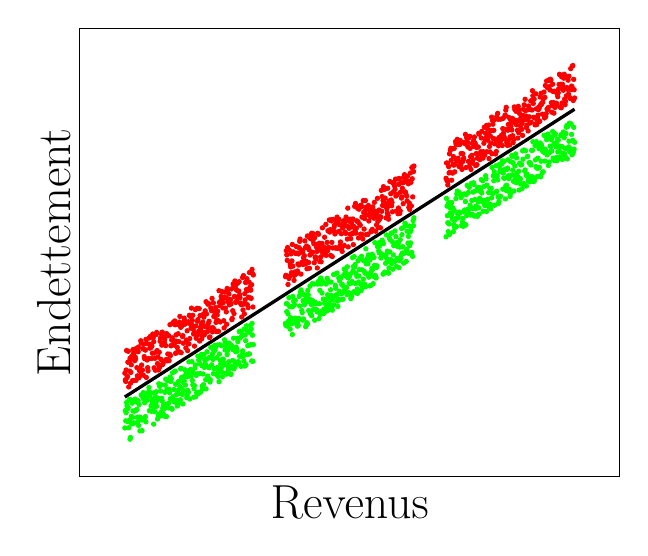
\begin{tikzpicture}


\begin{axis}[xtick=\empty, ytick=\empty, xlabel={\LARGE Revenus}, ylabel={\LARGE Endettement}]
\myGlobalTransformation{0}{0};

% pauvres
\addplot [green, only marks, mark=*, samples=300, mark size=0.75,domain=-3:1]{rand+x};
\addplot [red, only marks, mark=*, samples=300, mark size=0.75,domain=-3:1]{rand+x+2.5};

%moyens
\addplot [green, only marks, mark=*, samples=300, mark size=0.75,domain=2:6]{rand+x};
\addplot [red, only marks, mark=*, samples=300, mark size=0.75,domain=2:6]{rand+x+2.5};

%riches
\addplot [green, only marks, mark=*, samples=300, mark size=0.75,domain=7:11]{rand+x};
\addplot [red, only marks, mark=*, samples=300, mark size=0.75,domain=7:11]{rand+x+2.5};

%frontière
\addplot [black, very thick, domain=-3:11] {x+1.25};
\end{axis}


\end{tikzpicture}
\caption{\label{fig:xdiff} Multi-modal wages and indebtedness data generating mechanism with $y = \{0,1\}$ classes displayed in \textcolor{red}{red} and \textcolor{green}{green} respectively.}
\end{figure}

The second failing situation is the counterpart of the first tailored data generating mechanism. This time, suppose the covariates wages and indebtedness are uniformly sampled. Suppose there is a third categorical feature ``wages source'' which is drawn uniformly from three levels: renters, salaried workers and self-employed. One could argue that renters' risk level do not depend on their indebtedness, which is typically low (and a higher one is a major red flag), salaried workers' risk level is positively correlated with their indebtedness ratio as was the case for the first introductory example (see Figure~\ref{fig:xdiff}) and self-employed people's risk level is negatively correlated with this indebtedness ratio (say, the higher their personal engagement, the higher the chances of success of their business). This example data generating mechanism is illustrated on Figure~\ref{fig:ydiff}. In this situation, and contrary to the first example, an unsupervised generative clustering algorithm like \gls{pca} would not partition the data and the \textit{Credit Scoring} practitioner would construct only one scorecard. This scorecard would have high model bias since it is too simple to accommodate for the variety of the data generating mechanism and consequently perform poorly. This particular data generating mechanism is also revisited in the Experiments of Section~\ref{subsec:num_sim}.


\begin{figure}
\centering
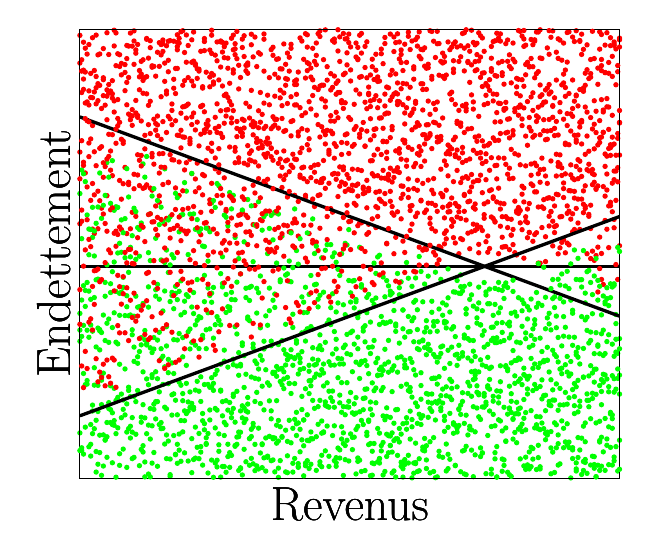
\begin{tikzpicture}


\begin{axis}[xtick=\empty, ytick=\empty, xlabel={\LARGE Revenus}, ylabel={\LARGE Endettement},domain=-3:1, enlargelimits=false,ymin=-3,ymax=6]
\myGlobalTransformationbis{0}{0};

% techniciens
\addplot [green, only marks, mark=*, samples=300, mark size=0.75,domain=-3:1]{rand};
\addplot [green, only marks, mark=*, samples=300, mark size=0.75,domain=-3:1]{rand-2};
\addplot [green, only marks, mark=*, samples=300, mark size=0.75,domain=-3:1]{rand-4};
\addplot [red, only marks, mark=*, samples=300, mark size=0.75,domain=-3:1]{rand+2.5};
\addplot [red, only marks, mark=*, samples=300, mark size=0.75,domain=-3:1]{rand+4.5};
\addplot [red, only marks, mark=*, samples=300, mark size=0.75,domain=-3:1]{rand+6.5};

%frontière
\addplot [black, very thick, domain=-3:1] {1.25};
\end{axis}





\begin{axis}[xtick=\empty, ytick=\empty, xlabel={\LARGE Revenus}, ylabel={\LARGE Endettement},domain=-3:1, enlargelimits=false,ymin=-3,ymax=6]
\myGlobalTransformationbis{0}{3};

% cadres
\addplot [green, only marks, mark=*, samples=300, mark size=0.75,domain=-3:1]{rand-x};
\addplot [green, only marks, mark=*, samples=300, mark size=0.75,domain=-3:1]{rand-x-2};
\addplot [green, only marks, mark=*, samples=300, mark size=0.75,domain=-3:1]{rand-x-4};
\addplot [red, only marks, mark=*, samples=300, mark size=0.75,domain=-3:1]{rand-x+2.5};
\addplot [red, only marks, mark=*, samples=300, mark size=0.75,domain=-3:1]{rand-x+4.5};
\addplot [red, only marks, mark=*, samples=300, mark size=0.75,domain=-3:1]{rand-x+6.5};

%frontière
\addplot [black, very thick, domain=-3:1] {-x+1.25};
\end{axis}



\begin{axis}[xtick=\empty, ytick=\empty, xlabel={\LARGE Revenus}, ylabel={\LARGE Endettement},domain=-3:1, enlargelimits=false,ymin=-3,ymax=6]
\myGlobalTransformationbis{0}{6};

% libérales
\addplot [green, only marks, mark=*, samples=300, mark size=0.75,domain=-3:1]{rand+x};
\addplot [green, only marks, mark=*, samples=300, mark size=0.75,domain=-3:1]{rand+x-2};
\addplot [green, only marks, mark=*, samples=300, mark size=0.75,domain=-3:1]{rand+x-4};
\addplot [red, only marks, mark=*, samples=300, mark size=0.75,domain=-3:1]{rand+x+2.5};
\addplot [red, only marks, mark=*, samples=300, mark size=0.75,domain=-3:1]{rand+x+4.5};
\addplot [red, only marks, mark=*, samples=300, mark size=0.75,domain=-3:1]{rand+x+6.5};
\addplot [red, only marks, mark=*, samples=300, mark size=0.75,domain=-3:1]{rand+x+8.5};

%frontière
\addplot [black, very thick, domain=-3:1] {x+1.25};
\end{axis}



\end{tikzpicture}
\caption{\label{fig:ydiff} Uni-modal wages and indebtedness data generating mechanism with $y = \{0,1\}$ classes displayed in \textcolor{red}{red} and \textcolor{green}{green} respectively which depends on a third feature.}
\end{figure}








\section{Literature review} \label{sec:literature}

This Section aims at providing an eluded literature review of some well-known supervised clustering approaches that could be transposed to the \textit{Credit Scoring} industry.

\subsection{Clustering methods}

In the preceding Section, examples of classical unsupervised clustering methods were given: \gls{pca} (continuous data), \gls{mca} (categorical data) and ultimately \gls{famd} (mixed data). In this Section, focus is given to supervised generative methods. Indeed, a fully generative model $p(\glssymbol{bx},y)$, if sufficiently flexible, could have easily spotted the bottlenecks of the failures of the \gls{pca} approach illustrated on Figures~\ref{fig:xdiff} and~\ref{fig:ydiff}.

\paragraph{\gls{pls}}

The \gls{pls}~\cite{wold1984collinearity} algorithm seeks to combine the strengths, in its original proposal, of \gls{pca} in explaining the variance of the features $\glssymbol{bx}$ and regression in predicting $y$ with the resulting principal components. In a classification setting, it is termed PLS-DA where DA stands for discriminant analysis.

The main idea is to construct a first component of the sum of the univariate regressions of $\glssymbol{bbx}_j$ on $\glssymbol{bby}$, then a second component of the sum of the univariate regressions of $\glssymbol{bbx}_j$ subtracted by the first component on $\glssymbol{bby}$, and so on. In a sense, a tradeoff between reconstruction quality of $\glssymbol{bbx}$ and $\glssymbol{bby}$ with as few components as possible is achieved.

The \gls{pls} algorithm is given in Section~\ref{alg:pls}, Algorithm~\ref{app1:sec_pls}.

\paragraph{\gls{spc}}

The \gls{spc}~\cite{bair2006prediction} algorithm is motivated by genomics applications where $d > n$, but is applicable to our current setting as well, and by the fact that, in a predictive setting, variance of the features $\glssymbol{bx}$ is only interesting if correlated with $y$. The inner-workings of the algorithm are relatively simple: the correlation between each feature $x_j$ and $y$ is computed. Only the features for which this correlation exceeds a user-defined threshold are retained, and the first few principal components of these features are calculated and used to predict $y$.

There is a close link between \gls{pls} and \gls{spc} that is thoroughly explained in~\cite{friedman2001elements} Section 18.6.2 p.\ 680.

For numerical experiments of Section~\ref{sec:num_exp}, we will use, among others, the \gls{pls} approach.

Although these methods make good use of $y$ in constructing sub-populations on which the practitioner would construct separate scorecards, the resulting segments would be, as described in the \gls{mca} Section, visually separated clouds of points on the graph of the two first principal components. This paradigm has two major drawbacks: first, as explained in the preceding Section, the separation boundary is complex and multivariate (as the two first principal components will most likely involve all features). Second, to make a complete tree as on Figure~\ref{fig:arbre}, these procedures would have to be repeated ``recursively'' which yields the need for a stopping criterion and an objective splitting criterion in place of the rather subjective visual separation. Direct approaches of estimating such trees are reviewed in the next Section.

\subsection{Direct approaches: logistic regression trees} \label{subsec:sup_gen}

\paragraph{\gls{lotus}}

The first research work focusing on a similar problem than the present one seems to be \gls{lotus}~\cite{chan2004lotus}, where logistic regression trees are constructed so as to select features to split the data on the tree's nodes which break the linearity assumption of \gls{lr}. The original article states an application case similar to this one, namely the insurance market.

Their motivation is that \gls{lr} has a fixed parameter space, defined by the number of input features, whereas trees adapt their flexibility (\textit{i.e.}\ depth) to the sample size $n$; however, trees perform well for classification (\textit{i.e.}\ by setting $\hat{y} = \argmax_y p(y | \glssymbol{bx})$ they can achieve low classification error) but poorly in assessing the probability of the event (\textit{i.e.}\ the estimate of $p(y | \glssymbol{bx})$ is the proportion of the event $y$ among observations $\glssymbol{bx}$ at each leaf) as it is piecewise constant; if the true decision boundary separating the two classes of $y$ given $\glssymbol{bx}$ is linear, they need an infinite depth to estimate it as well as \gls{lr}. Thus, they search for trees which leaves are \gls{lr} with a few continuous features and which intermediate nodes split the population based on categorical or continuous features which relationship to the log-odd ratio of $y$ is not linear (\textit{i.e.}\ features that would perform poorly in a \gls{lr}).

They propose a feature selection method for node splits that is bias-free: as seen in Chapters~\ref{chap4} and~\ref{chap5}, the number of partitions of $l_j$ labelled factor levels into $m_j$ unlabelled categories (which would here be the tree split criterion and define its sub-populations) is huge which yields overfitting; thus, their approach relies on a $\chi^2$ test which degrees of freedom is linked to the number of potential rearrangements of $l_j$ into 2 bins. Their optimized criterion is the sum of the log-likelihoods of the \gls{lr} on the tree's leaves. Of course, this leads also to overfitting which requires the tree to be pruned (as is classical for classification trees) using a method closely related to the one developed in the classical CART~\cite{cart84} algorithm. Lastly, their proposed method is not directly applicable to missing values: these observations are not used during training (in the \textit{Credit Scoring} industry, there would most likely be at least one missing value for each observation) and during test, their missing values are imputed by the mean or median.

To sum up, although their motivation is similar to the present problem, \gls{lotus} is not directly usable since only continuous features are used as predictive features in the \gls{lr} of the tree's leaves, it does not handle missing values gracefully, and there are currently no implementation available in \textsf{R} or Python.

\paragraph{\gls{lmt}}

The second approach very close to our industrial problem is named \gls{lmt}~\cite{landwehr2005logistic}. As for~\gls{lotus}, the result is a tree of \gls{lr} at its leaves and the motivation is very similar. Their introductory example, reproduced here with permission on Figure~\ref{fig:lmt} is enlightening: a quadratic boundary cannot be well approximated by trees or \gls{lr} alone, but a combination of both achieves good performance and interpretation.

Their approach differs however drastically from \gls{lotus} in that they rely on a particular boosting approach derived from the LogitBoost algorithm~\cite{friedman2000additive} to adjust the \gls{lr}, and an adaptation of the classical C4.5 algorithm to grow the tree. The two central ideas behind their usage of the LogitBoost algorithm are simple: it allows to perform feature selection \textit{via} a stagewise-like process where one feature enters the model at each step and to ``refine'' recursively the \gls{lr} by boosting the \gls{lr} fitted at a node's parent. Indeed, a first \gls{lr} is fitted at the tree's root via LogitBoost using all observations $(\glssymbol{bbx},\glssymbol{bby})$, which is further boosted separatly at its subsequent children nodes on sub-populations, say $((\glssymbol{bbx}^1,\glssymbol{bby}^1), (\glssymbol{bbx}^2,\glssymbol{bby}^2))$ and so on. This most probably induces less parameter estimation variance in each leaf since they partly benefit from samples not in their leaf but used to fit the parents' \gls{lr}. One if its main advantages compared to other approaches is that it is fast. Here again, the resulting tree must be pruned and a tactic similar to CART~\cite{cart84}, or cross-validation, or the AIC criterion (in a refinement proposed in~\cite{sumner2005speeding}) are used.

However, categorical features are dummy / one-hot encoded so that only a few factor levels might be selected at each leaf, which amounts to merging the not selected levels into a reference value. Conversely, when used as a split feature, each level yields a distinct branch. Moreover, missing values are imputed by the mean or mode.

Its original implementation is in Weka but \textsf{R} packages \rinline{party} and \rinline{partykit} provide interfaces and wrappers to it.

\begin{figure}[!htb]
{\setlength{\parindent}{0cm}}
\begin{center}
%\begin{multicols}{3}
\centering
\begin{subfigure}[t]{0.25\textwidth}
\centering
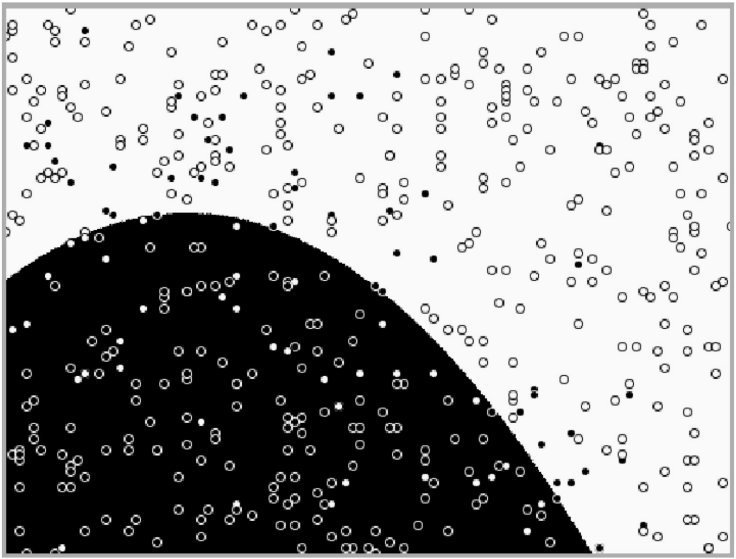
\includegraphics[width=\textwidth]{figures/chapitre6/lmt_generation.png}
\caption{\label{fig:lmt1} Quadratic data generation process: the true boundary depends on the square of input features.}
\end{subfigure}%
%\columnbreak
\hspace*{1cm}
\begin{subfigure}[t]{0.25\textwidth}
\centering
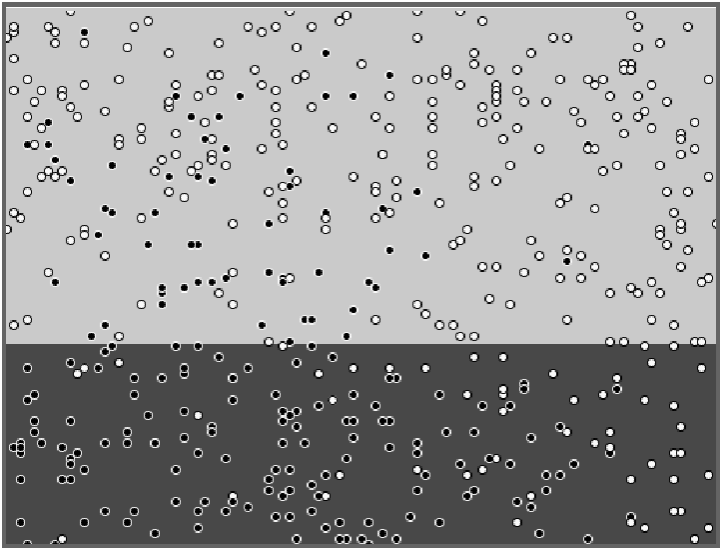
\includegraphics[width=\textwidth]{figures/chapitre6/lmt_tree_1.png}
\caption{\label{fig:lmt2} The first split of a classification tree like is way too simplistic.}
\end{subfigure}
%\columnbreak
\hspace*{1cm}
\begin{subfigure}[t]{0.25\textwidth}
\centering
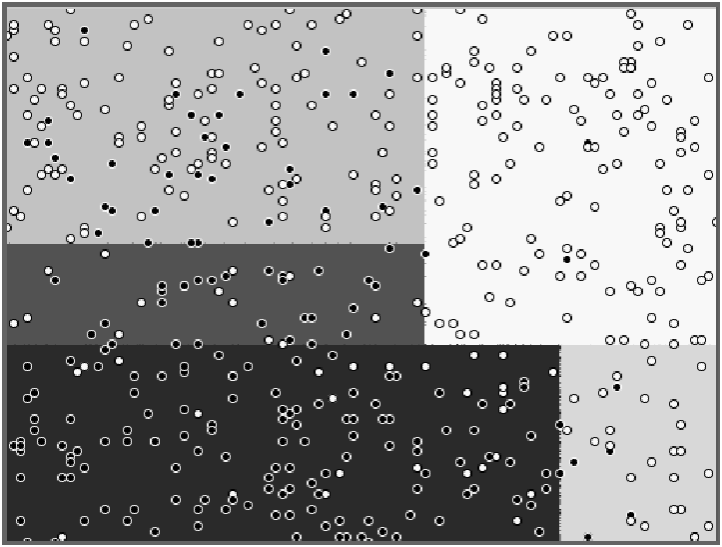
\includegraphics[width=\textwidth]{figures/chapitre6/lmt_tree_2.png}
\caption{\label{fig:lmt3}  The second split is more helpful.}
\end{subfigure}
%\end{multicols}
\end{center}

\begin{center}
%\begin{multicols}{2}
\centering
\begin{subfigure}[t]{0.32\textwidth}
\centering
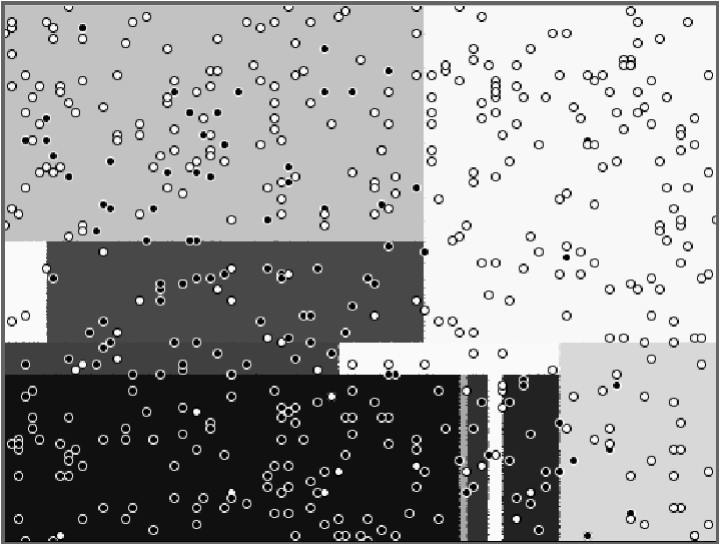
\includegraphics[width=\textwidth]{figures/chapitre6/lmt_tree_3.png}
\caption{\label{fig:lmt4} The third split yields overfitting: these nodes shall be pruned.}
\end{subfigure}%
%\columnbreak
\hspace*{1cm} \begin{subfigure}[t]{0.32\textwidth}
\centering
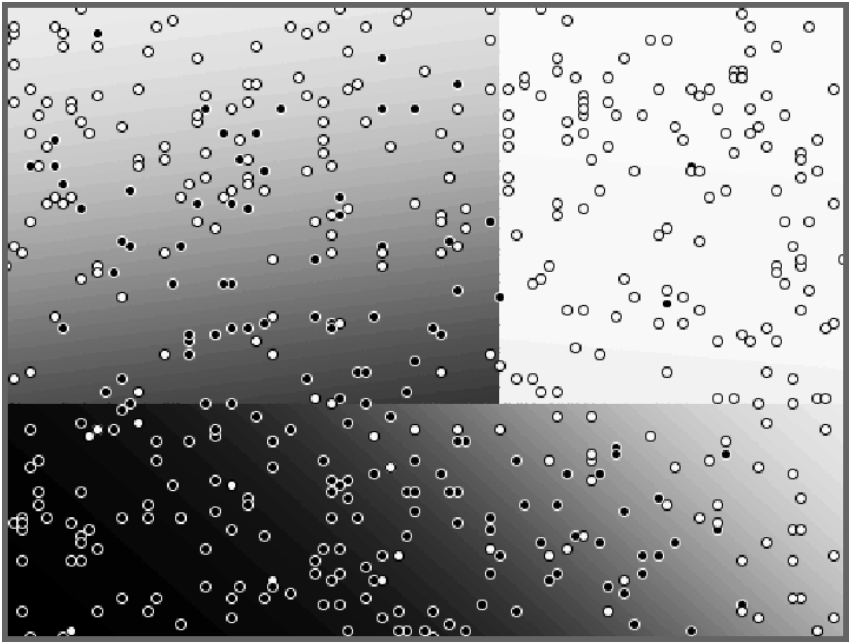
\includegraphics[width=\textwidth]{figures/chapitre6/lmt_logistic.png}
\caption{\label{fig:lmt5} A \gls{lr} tree with only two leaves (and consequently two \gls{lr}) yields the best result.}
\end{subfigure}
%\end{multicols}
\end{center}

\caption{\label{fig:lmt} LMT motivational example.}
\end{figure}




\paragraph{\gls{mob}} \label{par:mob}

Lastly, a third approach closely related to our problem is \gls{mob}~\cite{zeileis2008model} which is an adaptation of a better-known paper~\cite{hothorn2006unbiased} to parametric models in the leaves of a recursively partitioned dataset (hence the name).

Their algorithm consists in fitting the chosen model (in our case, \gls{lr}) for all observations $(\glssymbol{bbx},\glssymbol{bby})$ at the current node and decide to split these into subsets based on a correlation measure (several such measures are proposed) of the residuals of the current model and splitting features $\bm{V} = (V_1, \dots, V_p)$ where $V_j \in \glssymbol{R}$ or $\glssymbol{NO}$, $1 \leq j \ leq p$, which are not included in $\glssymbol{bbx}$. The procedure is repeated until no significant ``correlation'' is detected. The C4.5 algorithm, in presence of a binary outcome, orders the levels of categorical features by their proportion of events $y$ and split as if the feature were ordinal (it can be shown that it is optimal, see~\cite{friedman2001elements} Section 9.2.4).  Similarly to \gls{lotus} and contrary to C4.5, \gls{mob} performs $2^{l_j}$ tests for example for binary splits with categorical features $j$ of $l_j$ levels. Moreover, there is no mention to eventual treatment of missing values. The number of segments per split is searched exhaustively.

Its implementation is available through the \textsf{R} packages \rinline{party} and \rinline{partykit} which will be used in numerical experiments of Section~\ref{sec:num_exp}.

To sum up, these direct approaches are far more promising than unsupervised and supervised generative approaches of Sections~\ref{subsec:adhoc} and~\ref{subsec:sup_gen} respectively, in that they produce directly the sought tree-structure of Figure~\ref{fig:arbre} (apart of course from quantization $\q$). However, their treatment of missing values and categorical features are not satisfactory: classical \textit{Credit Scoring} data would require preprocessing steps such as imputation or quantization (or at least merging numerous factor levels) which might greatly influence the resulting segmentation as emphasized in Section~\ref{subsec:context}. Moreover, quantization has to be segment-specific: on a theoretical note, it participates in reducing model bias; on a practical note, it does not make much sense to use the same quantization of wages on segments of Ferrari leasing and smartphone leasing.

In the next Section, we formalize the problem as a model selection problem, similarly to the three approaches presented here, with our own notations introduced in the previous Section and Chapters.


\section{Logistic regression trees as a combinatorial model selection problem} \label{sec:model_selec_tree}

In this Section, it is supposed the well-specified model is indeed a \gls{lr} tree, which amounts to assuming there $K^\star$ segments. The membership of an observation $\glssymbol{bx}$ to a segment $c$ is given by a tree. We restrict to binary trees for simplicity, such that a segment $c$ has $r = 1, \dots, \mathcal{D}(c)$ parents successively denoted by $\mathcal{P}a^r(c)$. At these parent nodes, a binary rule is taken. This rule is univariate: it depends on only one feature $x_{\sigma(r,c)}$ where $\sigma(r,c)$ denotes the anti-rank of the feature used in rule $r$ for segment $c$. Being a binary rule, the membership of $x_{\sigma(r,c)}$ is tested between $C_{\mathcal{P}a^r(c),1}$ and $C_{\mathcal{P}a^r(c),2}$ such that $C_{\mathcal{P}a^r(c),1} \bigsqcup C_{\mathcal{P}a^r(c),2} =\glssymbol{R}$ for continuous features (half-spaces), or $\glssymbol{N}_{l_{\sigma(r,c)}}$ for categorical features respectively. The `unique `side'' $1$ or $2$ of rule $r$ that yields eventually to $c$ is denoted by $\lambda(r,c)$. With all these newly introduced notations, the probability of a segment $c$ given covariates $\glssymbol{bx}$ can be expressed as:
\begin{equation} \label{eq:tree}
p( c | \glssymbol{bx}) = \prod_{r = 1}^{\mathcal{D}(c)} \mathds{1}_{C_{\mathcal{P}a^r(c),\lambda(r,c)}} (x_{\sigma(r,c)})
\end{equation}
%where $r$ denotes the inverse depth of each rule relative to $c$ ($r=\ln_2 K$ gives the root rule, and so on) and $\sigma(r,c)$ gives the anti-rank of the feature used in rule $r$, at node $\mathcal{P}a^r(c)$, $C_{\mathcal{P}a^r(c),\lambda(r,c)} = \begin{cases} ]-\infty ; \lambda_r] \\ \text{or} \\ ] \lambda_r ; +\infty[ \end{cases}$ for a continuous feature and $C_{r,c} = \begin{cases} \lambda_{r,1} \\ \text{or} \\ \lambda_{r,2} \end{cases}$ such that $ \lambda_{r,1} \bigsqcup \lambda_{r,2} = \glssymbol{N}_{l_{\sigma(r)}}$ for a categorical feature depending on the ``side'' of the segment $c$ w.r.t.\ the rule $r$.
An example is given on Figure~\ref{fig_arbre_ex_notations}.
In each segment, the well-specified assumption is equivalent to a \gls{lr}:
\begin{equation} \label{eq:lr_tree}
\forall \glssymbol{bx}, y, \exists c^\star \in \glssymbol{N}_{K^\star}, \glssymbol{bth}^{\star,c^\star}, p(y | \glssymbol{bx}) = p_{\glssymbol{bth}^{\star,c^\star}}(y | \glssymbol{bx}, c^\star)
\end{equation}
For $c \in \glssymbol{N}_{K^\star}$, $(\glssymbol{bbx}^c, \glssymbol{bby}^c)$ denotes the subset of observations of $(\glssymbol{bbx}, \glssymbol{bby})$ for which $c^\star = c$, such that $ \bigsqcup_{c=1}^{K} (\glssymbol{bbx}^c, \glssymbol{bby}^c) = (\glssymbol{bbx}, \glssymbol{bby})$.

\tikzstyle{level 1}=[level distance=2.2cm, sibling distance=8cm]
\tikzstyle{level 2}=[level distance=2cm, sibling distance=4cm]


\begin{figure}
\resizebox{\textwidth}{!}{
\centering
\begin{tikzpicture}
  [
    sibling distance        = 15em,
    level distance          = 5em,
    edge from parent/.style = {draw, -latex},
    every node/.style       = {font=\footnotesize},
    sloped
  ]
  \node [root] {\textcolor{black}{$r = 2$}}
    child { node [dummy] {$r=1$}
      child { node [env] {\textcolor{black}{$c=1$ \hspace*{-0.4cm}}}
          edge from parent node [below] {$\glssymbol{x}_{\sigma(1,1)} \in C_{1,1}$} }
      child { node [env] {\textcolor{black}{$c=2$ \hspace*{-0.4cm}}}
              edge from parent node [above, align=center] {$\glssymbol{x}_{\sigma(1,1)} \not\in C_{1,2}$} }
              edge from parent node [above] {$\glssymbol{x}_{\sigma(2,1)} \in C_{2,1}$} }
    child { node [dummy] {$\cdot$}
      child { node [env] {\textcolor{black}{$c=3$ \hspace*{-0.4cm}}}
          edge from parent node [above] {$\cdot$} }
      child { node [env] {\textcolor{black}{$c=4$ \hspace*{-0.4cm}}}
              edge from parent node [above, align=center] {$\cdot$} }
              edge from parent node [above] {$\glssymbol{x}_{\sigma(2,1)} \not\in C_{2,2}$} };
\end{tikzpicture}
}
\caption{Notations by an example.}
\label{fig_arbre_ex_notations}
\end{figure}

The above mentioned \gls{lotus}, \gls{lmt} and \gls{mob} optimized the sum of the segments' log-likelihoods, then needed pruning since it leads to obvious overfitting: infinite log-likelihood is achievable by putting each sample into its own segment, provided there is at least one continuous feature and no identical examples with different labels, or combinations of categorical features' levels that separate classes perfectly.

Another approach can be taken by considering the segment $c$ as a latent random feature:
\begin{align}
p(\glssymbol{bbx},\glssymbol{bby}) & =  \sum_{c=1}^{K^\star} p(\glssymbol{bby} | \glssymbol{bbx}, c) p(c | \glssymbol{bbx}) p(\glssymbol{bbx}) & \text{(only $c = c^\star$ is non-zero)} \nonumber \\
 & = \prod_{c=1}^{K^\star} p(\glssymbol{bby}^c | \glssymbol{bbx}^c, c) p(\glssymbol{bbx}) \nonumber \\
 & = \prod_{c=1}^{K^\star} \int_{\Theta_c} p_{\glssymbol{bth}^{c}}(\glssymbol{bby}^c | \glssymbol{bbx}^c, c) p(\glssymbol{bth}^c | c) d\glssymbol{bth}^c p(\glssymbol{bbx}) \label{eq:likelihood_segment}
%\ln p(\glssymbol{bby}, \glssymbol{bbx}) & = \sum_{c=1}^{K^\star} \exp \left( \frac{-\text{BIC}(\hat{\glssymbol{bth}^c}) + O(1)}{2} \right) + \ln p(\glssymbol{bbx}) 
\end{align}
Consequently, the following criterion can be used to select a segmentation:
\begin{equation} \label{eq:BICc}
(K^\star, c^\star) = \argmin_{K,c} \sum_{c=1}^{K} \text{BIC}(\hat{\glssymbol{bth}}^c) + K - 1
\end{equation}
As was thoroughly explained for quantizations and interactions in Sections~\ref{par:consistency} and~\ref{sec:pairwise} respectively, it is unclear how many parameters should be accounted for in this BIC criterion since the tree of Equation~\eqref{eq:tree} has parameters $C_{\cdot,\cdot}$ which have to be estimated (this is somewhat reflected in Equation~\eqref{eq:likelihood_segment} by the $p(\glssymbol{bth}^c | c)$ term); some are continuous (when the split is done on a continuous feature), some are discrete (when it concerns a categorical feature). As discussed in Section~\ref{par:consistency}, discrete parameters are usually not counted, but here, following the C4.5 approach of considering the levels of categorical features as ordered (w.r.t.\ the proportion of events $y$ associated to them - see Section~\ref{subsec:sup_gen}, Paragraph~\nameref{par:mob}), a split on categorical features can count as one continuous parameter. This yields the $K-1$ term in Criterion~\eqref{eq:BICc}. However, when there are more than two classes $c$ (typically, a financial institution of moderate to big size would have $K = 4$ to $30$ scorecards), this ``ordering'' simplification about the search for discrete parameters does not apply. We still stick with criterion~\ref{eq:BICc} as it will show good empirical properties in Section~\ref{sec:num_exp}.


In the next Section, we propose to relax the constraint of Equation~\eqref{eq:tree}, exactly as was done for quantizations in Chapter~\ref{chap4}, by using a continuous approximation of this discrete (and thus highly difficult to directly optimize) problem.


\section{A mixture and latent feature-based relaxation}

The difficulty in optimising Criterion~\eqref{eq:BICc} directly lies in the discrete nature of $c$ given $\glssymbol{bx}$, illustrated by the profusion of indicator functions in Equation~\eqref{eq:tree}, which is very similar to the problems of quantization (see Chapter~\ref{chap4} and in particular Section~\ref{subsec:relaxation}) and interaction screening (see Chapter~\ref{chap5} and in particular Section~\ref{subsec:mcmc}). In both cases, highly-combinatorial discrete problems were relaxed, either by approaching door functions by softmax or . Unsurprisingly, a similar approach can be taken here for having a smooth approximation of $p(c | \glssymbol{bx})$ which will be denoted by $p_{\betag}(c | \glssymbol{bx})$.

\subsection{The proposed relaxation: tree structure and piecewise constant membership probability}

As emphasized in Section~\ref{subsec:sup_gen}, classification trees aim at predicting $c$ by making their leaves as ``pure'' (hence the use of the term impurity measure) as possible, \textit{i.e.}\ where one class strongly dominates the others by being the labels of most observations that fall into it. However, as for \gls{lr}, they can be viewed as ``statistical'' classifiers by substituting their classical majority vote by the proportion of each class in each leaf:
\begin{equation}
p_{\betag}(c | \glssymbol{bx}) = \frac{|\mathbf{c}^{\mathcal{L}(\glssymbol{bx})}|}{|\glssymbol{bbx}^{\mathcal{L}(\glssymbol{bx})}|},
\end{equation}
where $\mathcal{L}(\glssymbol{bx})$ denotes the leaf where $\glssymbol{bx}$ falls. Indeed, in this soft assignment, $\mathcal{L}(\glssymbol{bbx})$ and its segment $c$ are not identifiable. An example of such behaviour is given on Figure~\ref{fig:titanic_tree} where there are two classes: ``survived'' and ``not survived'' for Titanic passengers given their age, sex and passenger class. The proportion of each class in each leaf is given in parentheses.

\begin{figure}
\resizebox{\textwidth}{!}{% Created by tikzDevice version 0.12 on 2019-03-01 10:09:53
% !TEX encoding = UTF-8 Unicode
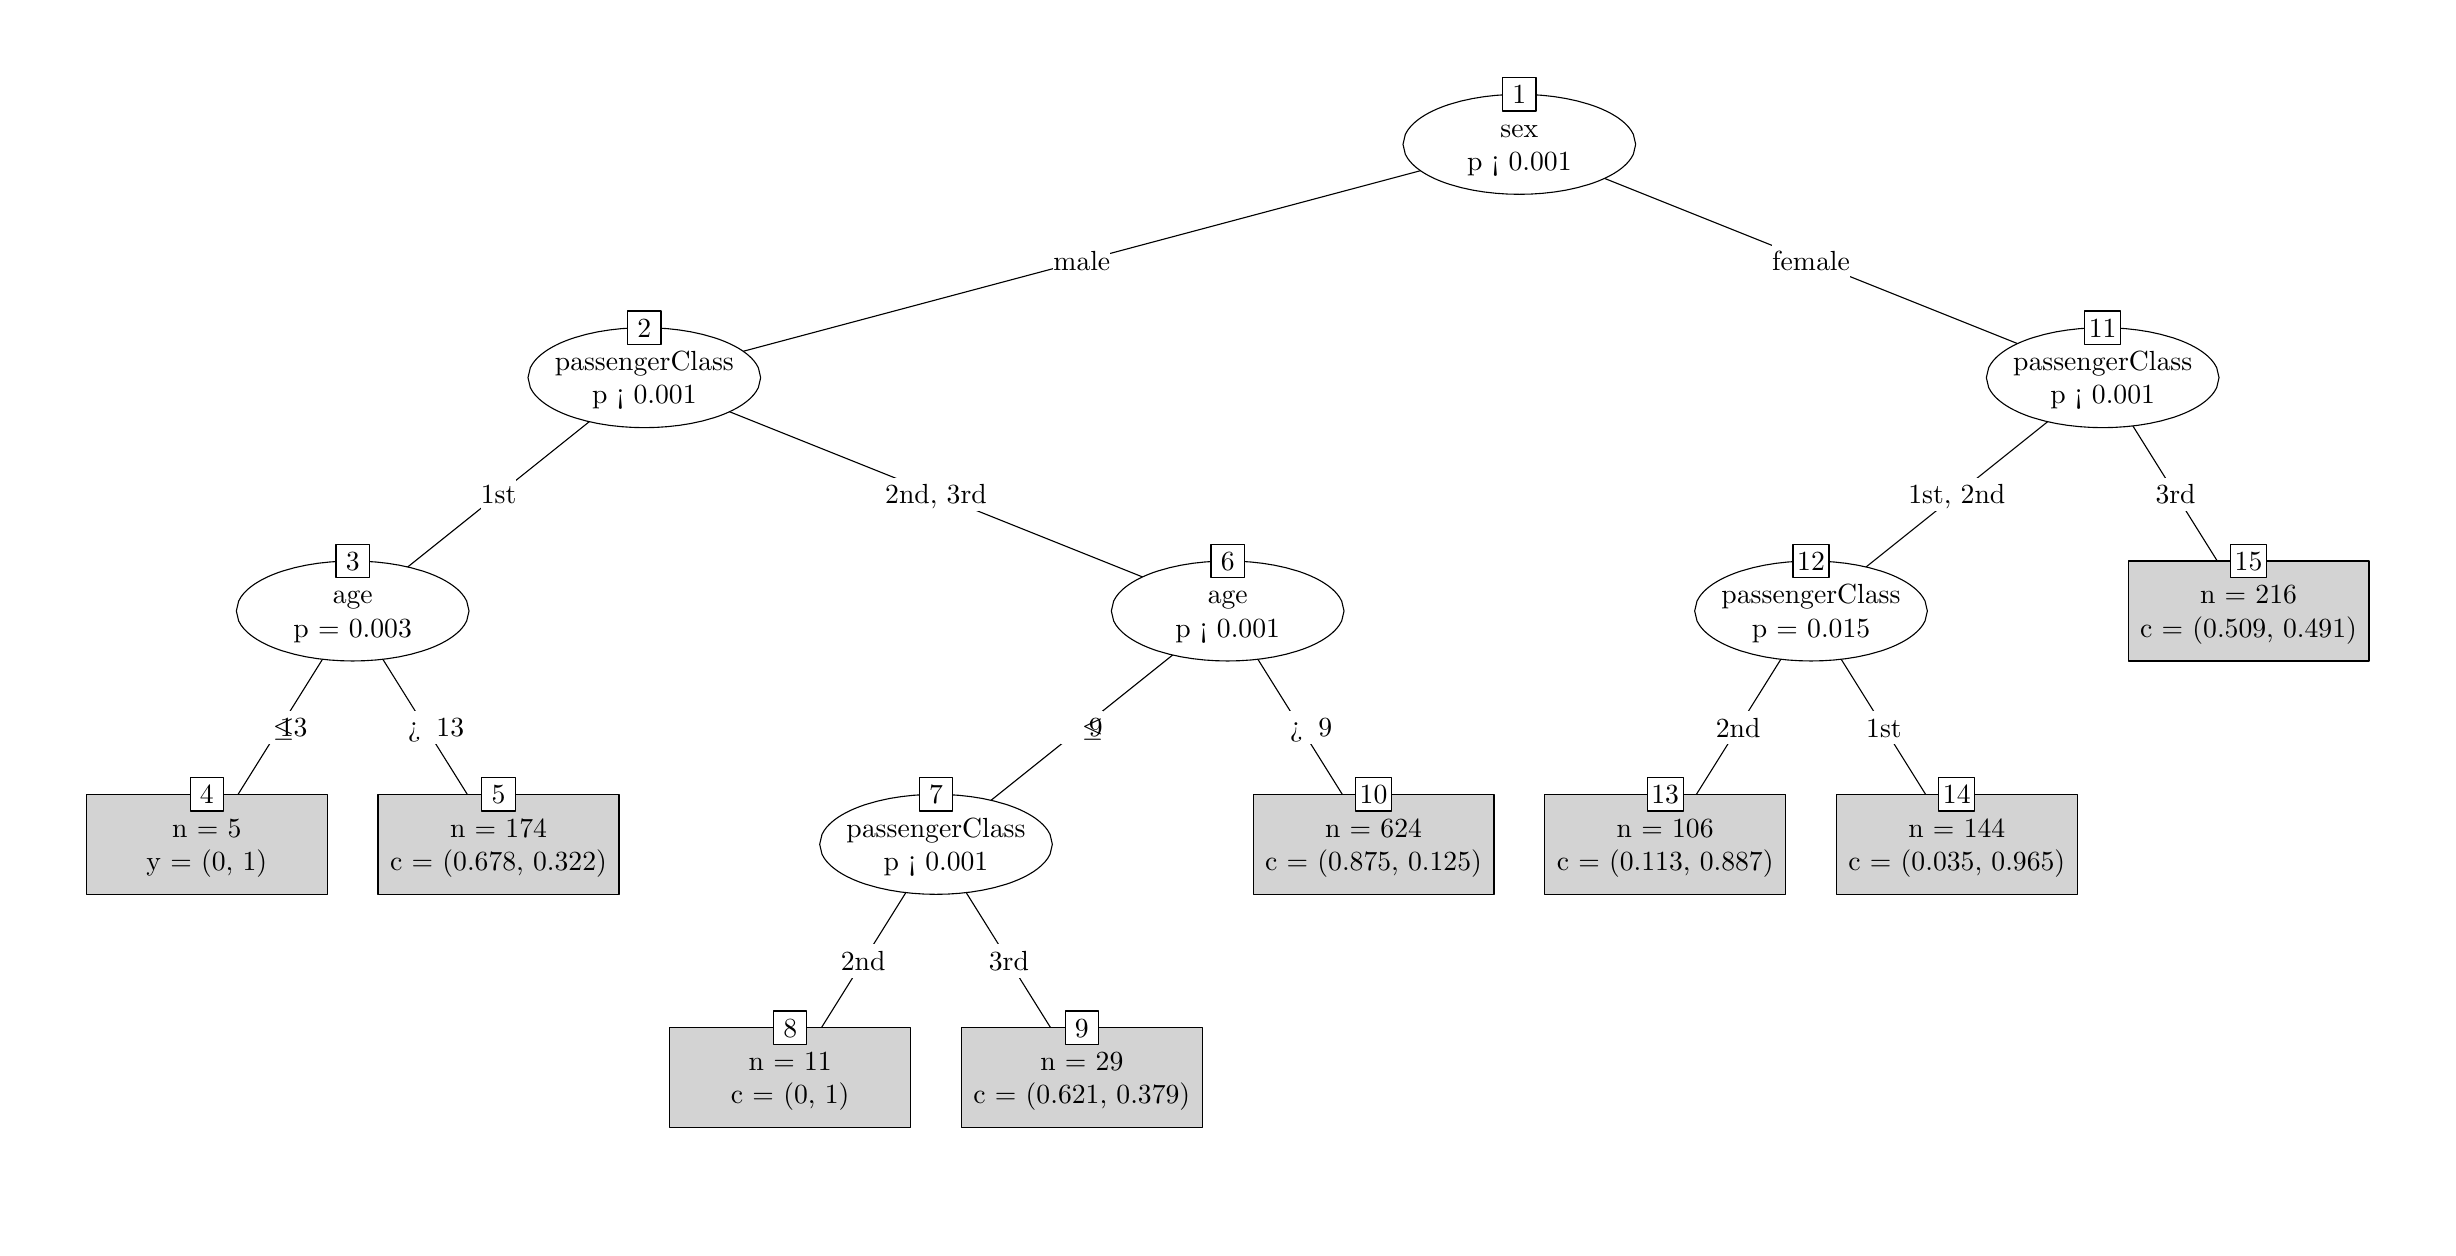
\begin{tikzpicture}[x=1pt,y=1pt]
\definecolor{fillColor}{RGB}{255,255,255}
\path[use as bounding box,fill=fillColor,fill opacity=0.00] (0,0) rectangle (867.24,433.62);
\begin{scope}
\path[clip] (  0.00,  0.00) rectangle (867.24,433.62);
\definecolor{drawColor}{RGB}{0,0,0}

\path[draw=drawColor,line width= 0.4pt,line join=round,line cap=round] (539.01,391.46) --
	(222.83,307.15);

\path[draw=drawColor,line width= 0.4pt,line join=round,line cap=round] (539.01,391.46) --
	(749.80,307.15);
\definecolor{fillColor}{RGB}{255,255,255}

\path[draw=drawColor,line width= 0.4pt,line join=round,line cap=round,fill=fillColor] (496.97,391.46) --
	(497.81,395.06) --
	(498.65,396.52) --
	(499.50,397.63) --
	(500.34,398.54) --
	(501.18,399.34) --
	(502.02,400.04) --
	(502.86,400.68) --
	(503.70,401.27) --
	(504.54,401.80) --
	(505.38,402.30) --
	(506.22,402.77) --
	(507.06,403.20) --
	(507.90,403.61) --
	(508.74,404.00) --
	(509.58,404.37) --
	(510.43,404.71) --
	(511.27,405.04) --
	(512.11,405.35) --
	(512.95,405.64) --
	(513.79,405.92) --
	(513.79,405.92) --
	(517.99,407.11) --
	(522.20,408.02) --
	(526.40,408.70) --
	(530.61,409.16) --
	(534.81,409.44) --
	(539.01,409.53) --
	(543.22,409.44) --
	(547.42,409.16) --
	(551.63,408.70) --
	(555.83,408.02) --
	(560.03,407.11) --
	(564.24,405.92) --
	(564.24,405.92) --
	(565.08,405.64) --
	(565.92,405.35) --
	(566.76,405.04) --
	(567.60,404.71) --
	(568.44,404.37) --
	(569.28,404.00) --
	(570.12,403.61) --
	(570.97,403.20) --
	(571.81,402.77) --
	(572.65,402.30) --
	(573.49,401.80) --
	(574.33,401.27) --
	(575.17,400.68) --
	(576.01,400.04) --
	(576.85,399.34) --
	(577.69,398.54) --
	(578.53,397.63) --
	(579.37,396.52) --
	(580.21,395.06) --
	(581.05,391.46) --
	(581.05,391.46) --
	(580.21,387.87) --
	(579.37,386.40) --
	(578.53,385.30) --
	(577.69,384.38) --
	(576.85,383.59) --
	(576.01,382.88) --
	(575.17,382.24) --
	(574.33,381.66) --
	(573.49,381.12) --
	(572.65,380.62) --
	(571.81,380.16) --
	(570.97,379.72) --
	(570.12,379.31) --
	(569.28,378.92) --
	(568.44,378.56) --
	(567.60,378.22) --
	(566.76,377.89) --
	(565.92,377.58) --
	(565.08,377.29) --
	(564.24,377.01) --
	(564.24,377.01) --
	(560.03,375.82) --
	(555.83,374.90) --
	(551.63,374.23) --
	(547.42,373.76) --
	(543.22,373.49) --
	(539.01,373.40) --
	(534.81,373.49) --
	(530.61,373.76) --
	(526.40,374.23) --
	(522.20,374.90) --
	(517.99,375.82) --
	(513.79,377.01) --
	(513.79,377.01) --
	(512.95,377.29) --
	(512.11,377.58) --
	(511.27,377.89) --
	(510.43,378.22) --
	(509.58,378.56) --
	(508.74,378.92) --
	(507.90,379.31) --
	(507.06,379.72) --
	(506.22,380.16) --
	(505.38,380.62) --
	(504.54,381.12) --
	(503.70,381.66) --
	(502.86,382.24) --
	(502.02,382.88) --
	(501.18,383.59) --
	(500.34,384.38) --
	(499.50,385.30) --
	(498.65,386.40) --
	(497.81,387.87) --
	(496.97,391.46) --
	cycle;

\node[text=drawColor,anchor=base,inner sep=0pt, outer sep=0pt, scale=  1.00] at (539.01,394.04) {sex};

\node[text=drawColor,anchor=base,inner sep=0pt, outer sep=0pt, scale=  1.00] at (539.01,382.00) {p < 0.001};

\path[draw=drawColor,line width= 0.4pt,line join=round,line cap=round,fill=fillColor] (532.99,403.51) rectangle (545.04,415.55);

\node[text=drawColor,anchor=base,inner sep=0pt, outer sep=0pt, scale=  1.00] at (539.01,406.09) {1};
\end{scope}
\begin{scope}
\path[clip] (  0.00,  0.00) rectangle (867.24,433.62);
\definecolor{fillColor}{RGB}{255,255,255}

\path[fill=fillColor] (370.65,343.28) rectangle (391.20,355.33);
\definecolor{drawColor}{RGB}{0,0,0}

\node[text=drawColor,anchor=base,inner sep=0pt, outer sep=0pt, scale=  1.00] at (380.92,345.86) {male};
\end{scope}
\begin{scope}
\path[clip] (  0.00,  0.00) rectangle (867.24,433.62);
\definecolor{fillColor}{RGB}{255,255,255}

\path[fill=fillColor] (630.38,343.28) rectangle (658.43,355.33);
\definecolor{drawColor}{RGB}{0,0,0}

\node[text=drawColor,anchor=base,inner sep=0pt, outer sep=0pt, scale=  1.00] at (644.41,345.86) {female};
\end{scope}
\begin{scope}
\path[clip] (  0.00,  0.00) rectangle (867.24,433.62);
\definecolor{drawColor}{RGB}{0,0,0}

\path[draw=drawColor,line width= 0.4pt,line join=round,line cap=round] (222.83,307.15) --
	(117.44,222.83);

\path[draw=drawColor,line width= 0.4pt,line join=round,line cap=round] (222.83,307.15) --
	(433.62,222.83);
\definecolor{fillColor}{RGB}{255,255,255}

\path[draw=drawColor,line width= 0.4pt,line join=round,line cap=round,fill=fillColor] (180.79,307.15) --
	(181.63,310.74) --
	(182.47,312.21) --
	(183.31,313.31) --
	(184.15,314.23) --
	(185.00,315.02) --
	(185.84,315.73) --
	(186.68,316.37) --
	(187.52,316.95) --
	(188.36,317.49) --
	(189.20,317.99) --
	(190.04,318.45) --
	(190.88,318.89) --
	(191.72,319.30) --
	(192.56,319.69) --
	(193.40,320.05) --
	(194.24,320.39) --
	(195.09,320.72) --
	(195.93,321.03) --
	(196.77,321.32) --
	(197.61,321.60) --
	(197.61,321.60) --
	(201.81,322.79) --
	(206.02,323.71) --
	(210.22,324.38) --
	(214.42,324.85) --
	(218.63,325.12) --
	(222.83,325.21) --
	(227.04,325.12) --
	(231.24,324.85) --
	(235.44,324.38) --
	(239.65,323.71) --
	(243.85,322.79) --
	(248.06,321.60) --
	(248.06,321.60) --
	(248.90,321.32) --
	(249.74,321.03) --
	(250.58,320.72) --
	(251.42,320.39) --
	(252.26,320.05) --
	(253.10,319.69) --
	(253.94,319.30) --
	(254.78,318.89) --
	(255.62,318.45) --
	(256.47,317.99) --
	(257.31,317.49) --
	(258.15,316.95) --
	(258.99,316.37) --
	(259.83,315.73) --
	(260.67,315.02) --
	(261.51,314.23) --
	(262.35,313.31) --
	(263.19,312.21) --
	(264.03,310.74) --
	(264.87,307.15) --
	(264.87,307.15) --
	(264.03,303.55) --
	(263.19,302.09) --
	(262.35,300.98) --
	(261.51,300.07) --
	(260.67,299.27) --
	(259.83,298.57) --
	(258.99,297.93) --
	(258.15,297.34) --
	(257.31,296.81) --
	(256.47,296.31) --
	(255.62,295.84) --
	(254.78,295.41) --
	(253.94,295.00) --
	(253.10,294.61) --
	(252.26,294.24) --
	(251.42,293.90) --
	(250.58,293.57) --
	(249.74,293.26) --
	(248.90,292.97) --
	(248.06,292.69) --
	(248.06,292.69) --
	(243.85,291.50) --
	(239.65,290.59) --
	(235.44,289.91) --
	(231.24,289.45) --
	(227.04,289.17) --
	(222.83,289.08) --
	(218.63,289.17) --
	(214.42,289.45) --
	(210.22,289.91) --
	(206.02,290.59) --
	(201.81,291.50) --
	(197.61,292.69) --
	(197.61,292.69) --
	(196.77,292.97) --
	(195.93,293.26) --
	(195.09,293.57) --
	(194.24,293.90) --
	(193.40,294.24) --
	(192.56,294.61) --
	(191.72,295.00) --
	(190.88,295.41) --
	(190.04,295.84) --
	(189.20,296.31) --
	(188.36,296.81) --
	(187.52,297.34) --
	(186.68,297.93) --
	(185.84,298.57) --
	(185.00,299.27) --
	(184.15,300.07) --
	(183.31,300.98) --
	(182.47,302.09) --
	(181.63,303.55) --
	(180.79,307.15) --
	cycle;

\node[text=drawColor,anchor=base,inner sep=0pt, outer sep=0pt, scale=  1.00] at (222.83,309.73) {passengerClass};

\node[text=drawColor,anchor=base,inner sep=0pt, outer sep=0pt, scale=  1.00] at (222.83,297.68) {p < 0.001};

\path[draw=drawColor,line width= 0.4pt,line join=round,line cap=round,fill=fillColor] (216.81,319.19) rectangle (228.85,331.24);

\node[text=drawColor,anchor=base,inner sep=0pt, outer sep=0pt, scale=  1.00] at (222.83,321.77) {2};
\end{scope}
\begin{scope}
\path[clip] (  0.00,  0.00) rectangle (867.24,433.62);
\definecolor{fillColor}{RGB}{255,255,255}

\path[fill=fillColor] (163.72,258.97) rectangle (176.55,271.01);
\definecolor{drawColor}{RGB}{0,0,0}

\node[text=drawColor,anchor=base,inner sep=0pt, outer sep=0pt, scale=  1.00] at (170.14,261.55) {1st};
\end{scope}
\begin{scope}
\path[clip] (  0.00,  0.00) rectangle (867.24,433.62);
\definecolor{fillColor}{RGB}{255,255,255}

\path[fill=fillColor] (309.88,258.97) rectangle (346.57,271.01);
\definecolor{drawColor}{RGB}{0,0,0}

\node[text=drawColor,anchor=base,inner sep=0pt, outer sep=0pt, scale=  1.00] at (328.23,261.55) {{2nd, 3rd}};
\end{scope}
\begin{scope}
\path[clip] (  0.00,  0.00) rectangle (867.24,433.62);
\definecolor{drawColor}{RGB}{0,0,0}

\path[draw=drawColor,line width= 0.4pt,line join=round,line cap=round] (117.44,222.83) --
	( 64.74,138.52);

\path[draw=drawColor,line width= 0.4pt,line join=round,line cap=round] (117.44,222.83) --
	(170.14,138.52);
\definecolor{fillColor}{RGB}{255,255,255}

\path[draw=drawColor,line width= 0.4pt,line join=round,line cap=round,fill=fillColor] ( 75.40,222.83) --
	( 76.24,226.43) --
	( 77.08,227.89) --
	( 77.92,229.00) --
	( 78.76,229.91) --
	( 79.60,230.71) --
	( 80.44,231.41) --
	( 81.28,232.05) --
	( 82.12,232.64) --
	( 82.97,233.17) --
	( 83.81,233.67) --
	( 84.65,234.14) --
	( 85.49,234.57) --
	( 86.33,234.98) --
	( 87.17,235.37) --
	( 88.01,235.74) --
	( 88.85,236.08) --
	( 89.69,236.41) --
	( 90.53,236.72) --
	( 91.37,237.01) --
	( 92.21,237.29) --
	( 92.21,237.29) --
	( 96.42,238.48) --
	(100.62,239.39) --
	(104.83,240.07) --
	(109.03,240.53) --
	(113.23,240.81) --
	(117.44,240.90) --
	(121.64,240.81) --
	(125.85,240.53) --
	(130.05,240.07) --
	(134.26,239.39) --
	(138.46,238.48) --
	(142.66,237.29) --
	(142.66,237.29) --
	(143.50,237.01) --
	(144.35,236.72) --
	(145.19,236.41) --
	(146.03,236.08) --
	(146.87,235.74) --
	(147.71,235.37) --
	(148.55,234.98) --
	(149.39,234.57) --
	(150.23,234.14) --
	(151.07,233.67) --
	(151.91,233.17) --
	(152.75,232.64) --
	(153.59,232.05) --
	(154.43,231.41) --
	(155.28,230.71) --
	(156.12,229.91) --
	(156.96,229.00) --
	(157.80,227.89) --
	(158.64,226.43) --
	(159.48,222.83) --
	(159.48,222.83) --
	(158.64,219.24) --
	(157.80,217.77) --
	(156.96,216.67) --
	(156.12,215.75) --
	(155.28,214.96) --
	(154.43,214.25) --
	(153.59,213.61) --
	(152.75,213.03) --
	(151.91,212.49) --
	(151.07,211.99) --
	(150.23,211.53) --
	(149.39,211.09) --
	(148.55,210.68) --
	(147.71,210.29) --
	(146.87,209.93) --
	(146.03,209.59) --
	(145.19,209.26) --
	(144.35,208.95) --
	(143.50,208.66) --
	(142.66,208.38) --
	(142.66,208.38) --
	(138.46,207.19) --
	(134.26,206.27) --
	(130.05,205.60) --
	(125.85,205.13) --
	(121.64,204.86) --
	(117.44,204.77) --
	(113.23,204.86) --
	(109.03,205.13) --
	(104.83,205.60) --
	(100.62,206.27) --
	( 96.42,207.19) --
	( 92.21,208.38) --
	( 92.21,208.38) --
	( 91.37,208.66) --
	( 90.53,208.95) --
	( 89.69,209.26) --
	( 88.85,209.59) --
	( 88.01,209.93) --
	( 87.17,210.29) --
	( 86.33,210.68) --
	( 85.49,211.09) --
	( 84.65,211.53) --
	( 83.81,211.99) --
	( 82.97,212.49) --
	( 82.12,213.03) --
	( 81.28,213.61) --
	( 80.44,214.25) --
	( 79.60,214.96) --
	( 78.76,215.75) --
	( 77.92,216.67) --
	( 77.08,217.77) --
	( 76.24,219.24) --
	( 75.40,222.83) --
	cycle;

\node[text=drawColor,anchor=base,inner sep=0pt, outer sep=0pt, scale=  1.00] at (117.44,225.41) {age};

\node[text=drawColor,anchor=base,inner sep=0pt, outer sep=0pt, scale=  1.00] at (117.44,213.37) {p = 0.003};

\path[draw=drawColor,line width= 0.4pt,line join=round,line cap=round,fill=fillColor] (111.42,234.88) rectangle (123.46,246.92);

\node[text=drawColor,anchor=base,inner sep=0pt, outer sep=0pt, scale=  1.00] at (117.44,237.46) {3};
\end{scope}
\begin{scope}
\path[clip] (  0.00,  0.00) rectangle (867.24,433.62);
\definecolor{fillColor}{RGB}{255,255,255}

\path[fill=fillColor] ( 81.05,174.65) rectangle (101.13,186.70);
\definecolor{drawColor}{RGB}{0,0,0}

\node[text=drawColor,anchor=base west,inner sep=0pt, outer sep=0pt, scale=  1.00] at ( 88.59,177.47) {$\leq$};

\node[text=drawColor,anchor=base west,inner sep=0pt, outer sep=0pt, scale=  1.00] at ( 91.14,177.47) {13};
\end{scope}
\begin{scope}
\path[clip] (  0.00,  0.00) rectangle (867.24,433.62);
\definecolor{fillColor}{RGB}{255,255,255}

\path[fill=fillColor] (129.86,174.65) rectangle (157.72,186.70);
\definecolor{drawColor}{RGB}{0,0,0}

\node[text=drawColor,anchor=base west,inner sep=0pt, outer sep=0pt, scale=  1.00] at (137.40,177.66) {>};

\node[text=drawColor,anchor=base west,inner sep=0pt, outer sep=0pt, scale=  1.00] at (147.72,177.66) {13};
\end{scope}
\begin{scope}
\path[clip] (  0.00,  0.00) rectangle (867.24,433.62);
\definecolor{drawColor}{RGB}{0,0,0}
\definecolor{fillColor}{RGB}{211,211,211}

\path[draw=drawColor,line width= 0.4pt,line join=round,line cap=round,fill=fillColor] ( 21.21,120.45) rectangle (108.27,156.59);

\node[text=drawColor,anchor=base,inner sep=0pt, outer sep=0pt, scale=  1.00] at ( 64.74,141.10) {n = 5};

\node[text=drawColor,anchor=base,inner sep=0pt, outer sep=0pt, scale=  1.00] at ( 64.74,129.05) {y = (0, 1)};
\definecolor{fillColor}{RGB}{255,255,255}

\path[draw=drawColor,line width= 0.4pt,line join=round,line cap=round,fill=fillColor] ( 58.72,150.56) rectangle ( 70.76,162.61);

\node[text=drawColor,anchor=base,inner sep=0pt, outer sep=0pt, scale=  1.00] at ( 64.74,153.14) {4};
\end{scope}
\begin{scope}
\path[clip] (  0.00,  0.00) rectangle (867.24,433.62);
\definecolor{drawColor}{RGB}{0,0,0}
\definecolor{fillColor}{RGB}{211,211,211}

\path[draw=drawColor,line width= 0.4pt,line join=round,line cap=round,fill=fillColor] (126.60,120.45) rectangle (213.67,156.59);

\node[text=drawColor,anchor=base,inner sep=0pt, outer sep=0pt, scale=  1.00] at (170.14,141.10) {n = 174};

\node[text=drawColor,anchor=base,inner sep=0pt, outer sep=0pt, scale=  1.00] at (170.14,129.05) {c = (0.678, 0.322)};
\definecolor{fillColor}{RGB}{255,255,255}

\path[draw=drawColor,line width= 0.4pt,line join=round,line cap=round,fill=fillColor] (164.11,150.56) rectangle (176.16,162.61);

\node[text=drawColor,anchor=base,inner sep=0pt, outer sep=0pt, scale=  1.00] at (170.14,153.14) {5};
\end{scope}
\begin{scope}
\path[clip] (  0.00,  0.00) rectangle (867.24,433.62);
\definecolor{drawColor}{RGB}{0,0,0}

\path[draw=drawColor,line width= 0.4pt,line join=round,line cap=round] (433.62,222.83) --
	(328.23,138.52);

\path[draw=drawColor,line width= 0.4pt,line join=round,line cap=round] (433.62,222.83) --
	(486.32,138.52);
\definecolor{fillColor}{RGB}{255,255,255}

\path[draw=drawColor,line width= 0.4pt,line join=round,line cap=round,fill=fillColor] (391.58,222.83) --
	(392.42,226.43) --
	(393.26,227.89) --
	(394.10,229.00) --
	(394.94,229.91) --
	(395.78,230.71) --
	(396.62,231.41) --
	(397.46,232.05) --
	(398.31,232.64) --
	(399.15,233.17) --
	(399.99,233.67) --
	(400.83,234.14) --
	(401.67,234.57) --
	(402.51,234.98) --
	(403.35,235.37) --
	(404.19,235.74) --
	(405.03,236.08) --
	(405.87,236.41) --
	(406.71,236.72) --
	(407.55,237.01) --
	(408.40,237.29) --
	(408.40,237.29) --
	(412.60,238.48) --
	(416.80,239.39) --
	(421.01,240.07) --
	(425.21,240.53) --
	(429.42,240.81) --
	(433.62,240.90) --
	(437.82,240.81) --
	(442.03,240.53) --
	(446.23,240.07) --
	(450.44,239.39) --
	(454.64,238.48) --
	(458.84,237.29) --
	(458.84,237.29) --
	(459.69,237.01) --
	(460.53,236.72) --
	(461.37,236.41) --
	(462.21,236.08) --
	(463.05,235.74) --
	(463.89,235.37) --
	(464.73,234.98) --
	(465.57,234.57) --
	(466.41,234.14) --
	(467.25,233.67) --
	(468.09,233.17) --
	(468.93,232.64) --
	(469.78,232.05) --
	(470.62,231.41) --
	(471.46,230.71) --
	(472.30,229.91) --
	(473.14,229.00) --
	(473.98,227.89) --
	(474.82,226.43) --
	(475.66,222.83) --
	(475.66,222.83) --
	(474.82,219.24) --
	(473.98,217.77) --
	(473.14,216.67) --
	(472.30,215.75) --
	(471.46,214.96) --
	(470.62,214.25) --
	(469.78,213.61) --
	(468.93,213.03) --
	(468.09,212.49) --
	(467.25,211.99) --
	(466.41,211.53) --
	(465.57,211.09) --
	(464.73,210.68) --
	(463.89,210.29) --
	(463.05,209.93) --
	(462.21,209.59) --
	(461.37,209.26) --
	(460.53,208.95) --
	(459.69,208.66) --
	(458.84,208.38) --
	(458.84,208.38) --
	(454.64,207.19) --
	(450.44,206.27) --
	(446.23,205.60) --
	(442.03,205.13) --
	(437.82,204.86) --
	(433.62,204.77) --
	(429.42,204.86) --
	(425.21,205.13) --
	(421.01,205.60) --
	(416.80,206.27) --
	(412.60,207.19) --
	(408.40,208.38) --
	(408.40,208.38) --
	(407.55,208.66) --
	(406.71,208.95) --
	(405.87,209.26) --
	(405.03,209.59) --
	(404.19,209.93) --
	(403.35,210.29) --
	(402.51,210.68) --
	(401.67,211.09) --
	(400.83,211.53) --
	(399.99,211.99) --
	(399.15,212.49) --
	(398.31,213.03) --
	(397.46,213.61) --
	(396.62,214.25) --
	(395.78,214.96) --
	(394.94,215.75) --
	(394.10,216.67) --
	(393.26,217.77) --
	(392.42,219.24) --
	(391.58,222.83) --
	cycle;

\node[text=drawColor,anchor=base,inner sep=0pt, outer sep=0pt, scale=  1.00] at (433.62,225.41) {age};

\node[text=drawColor,anchor=base,inner sep=0pt, outer sep=0pt, scale=  1.00] at (433.62,213.37) {p < 0.001};

\path[draw=drawColor,line width= 0.4pt,line join=round,line cap=round,fill=fillColor] (427.60,234.88) rectangle (439.64,246.92);

\node[text=drawColor,anchor=base,inner sep=0pt, outer sep=0pt, scale=  1.00] at (433.62,237.46) {6};
\end{scope}
\begin{scope}
\path[clip] (  0.00,  0.00) rectangle (867.24,433.62);
\definecolor{fillColor}{RGB}{255,255,255}

\path[fill=fillColor] (373.38,174.65) rectangle (388.47,186.70);
\definecolor{drawColor}{RGB}{0,0,0}

\node[text=drawColor,anchor=base west,inner sep=0pt, outer sep=0pt, scale=  1.00] at (380.92,177.47) {$\leq$};

\node[text=drawColor,anchor=base west,inner sep=0pt, outer sep=0pt, scale=  1.00] at (383.47,177.47) {9};
\end{scope}
\begin{scope}
\path[clip] (  0.00,  0.00) rectangle (867.24,433.62);
\definecolor{fillColor}{RGB}{255,255,255}

\path[fill=fillColor] (448.54,174.65) rectangle (471.40,186.70);
\definecolor{drawColor}{RGB}{0,0,0}

\node[text=drawColor,anchor=base west,inner sep=0pt, outer sep=0pt, scale=  1.00] at (456.08,177.66) {>};

\node[text=drawColor,anchor=base west,inner sep=0pt, outer sep=0pt, scale=  1.00] at (466.40,177.66) {9};
\end{scope}
\begin{scope}
\path[clip] (  0.00,  0.00) rectangle (867.24,433.62);
\definecolor{drawColor}{RGB}{0,0,0}

\path[draw=drawColor,line width= 0.4pt,line join=round,line cap=round] (328.23,138.52) --
	(275.53, 54.20);

\path[draw=drawColor,line width= 0.4pt,line join=round,line cap=round] (328.23,138.52) --
	(380.92, 54.20);
\definecolor{fillColor}{RGB}{255,255,255}

\path[draw=drawColor,line width= 0.4pt,line join=round,line cap=round,fill=fillColor] (286.19,138.52) --
	(287.03,142.11) --
	(287.87,143.58) --
	(288.71,144.68) --
	(289.55,145.60) --
	(290.39,146.39) --
	(291.23,147.10) --
	(292.07,147.74) --
	(292.91,148.32) --
	(293.75,148.86) --
	(294.59,149.36) --
	(295.43,149.82) --
	(296.27,150.26) --
	(297.12,150.67) --
	(297.96,151.06) --
	(298.80,151.42) --
	(299.64,151.76) --
	(300.48,152.09) --
	(301.32,152.40) --
	(302.16,152.69) --
	(303.00,152.97) --
	(303.00,152.97) --
	(307.21,154.16) --
	(311.41,155.08) --
	(315.61,155.75) --
	(319.82,156.22) --
	(324.02,156.49) --
	(328.23,156.58) --
	(332.43,156.49) --
	(336.63,156.22) --
	(340.84,155.75) --
	(345.04,155.08) --
	(349.25,154.16) --
	(353.45,152.97) --
	(353.45,152.97) --
	(354.29,152.69) --
	(355.13,152.40) --
	(355.97,152.09) --
	(356.81,151.76) --
	(357.66,151.42) --
	(358.50,151.06) --
	(359.34,150.67) --
	(360.18,150.26) --
	(361.02,149.82) --
	(361.86,149.36) --
	(362.70,148.86) --
	(363.54,148.32) --
	(364.38,147.74) --
	(365.22,147.10) --
	(366.06,146.39) --
	(366.90,145.60) --
	(367.74,144.68) --
	(368.59,143.58) --
	(369.43,142.11) --
	(370.27,138.52) --
	(370.27,138.52) --
	(369.43,134.92) --
	(368.59,133.46) --
	(367.74,132.35) --
	(366.90,131.44) --
	(366.06,130.64) --
	(365.22,129.94) --
	(364.38,129.30) --
	(363.54,128.71) --
	(362.70,128.18) --
	(361.86,127.68) --
	(361.02,127.21) --
	(360.18,126.78) --
	(359.34,126.37) --
	(358.50,125.98) --
	(357.66,125.61) --
	(356.81,125.27) --
	(355.97,124.94) --
	(355.13,124.63) --
	(354.29,124.34) --
	(353.45,124.06) --
	(353.45,124.06) --
	(349.25,122.87) --
	(345.04,121.96) --
	(340.84,121.28) --
	(336.63,120.82) --
	(332.43,120.54) --
	(328.23,120.45) --
	(324.02,120.54) --
	(319.82,120.82) --
	(315.61,121.28) --
	(311.41,121.96) --
	(307.21,122.87) --
	(303.00,124.06) --
	(303.00,124.06) --
	(302.16,124.34) --
	(301.32,124.63) --
	(300.48,124.94) --
	(299.64,125.27) --
	(298.80,125.61) --
	(297.96,125.98) --
	(297.12,126.37) --
	(296.27,126.78) --
	(295.43,127.21) --
	(294.59,127.68) --
	(293.75,128.18) --
	(292.91,128.71) --
	(292.07,129.30) --
	(291.23,129.94) --
	(290.39,130.64) --
	(289.55,131.44) --
	(288.71,132.35) --
	(287.87,133.46) --
	(287.03,134.92) --
	(286.19,138.52) --
	cycle;

\node[text=drawColor,anchor=base,inner sep=0pt, outer sep=0pt, scale=  1.00] at (328.23,141.10) {passengerClass};

\node[text=drawColor,anchor=base,inner sep=0pt, outer sep=0pt, scale=  1.00] at (328.23,129.05) {p < 0.001};

\path[draw=drawColor,line width= 0.4pt,line join=round,line cap=round,fill=fillColor] (322.20,150.56) rectangle (334.25,162.61);

\node[text=drawColor,anchor=base,inner sep=0pt, outer sep=0pt, scale=  1.00] at (328.23,153.14) {7};
\end{scope}
\begin{scope}
\path[clip] (  0.00,  0.00) rectangle (867.24,433.62);
\definecolor{fillColor}{RGB}{255,255,255}

\path[fill=fillColor] (293.82, 90.34) rectangle (309.93,102.38);
\definecolor{drawColor}{RGB}{0,0,0}

\node[text=drawColor,anchor=base,inner sep=0pt, outer sep=0pt, scale=  1.00] at (301.88, 92.92) {2nd};
\end{scope}
\begin{scope}
\path[clip] (  0.00,  0.00) rectangle (867.24,433.62);
\definecolor{fillColor}{RGB}{255,255,255}

\path[fill=fillColor] (347.34, 90.34) rectangle (361.81,102.38);
\definecolor{drawColor}{RGB}{0,0,0}

\node[text=drawColor,anchor=base,inner sep=0pt, outer sep=0pt, scale=  1.00] at (354.57, 92.92) {3rd};
\end{scope}
\begin{scope}
\path[clip] (  0.00,  0.00) rectangle (867.24,433.62);
\definecolor{drawColor}{RGB}{0,0,0}
\definecolor{fillColor}{RGB}{211,211,211}

\path[draw=drawColor,line width= 0.4pt,line join=round,line cap=round,fill=fillColor] (232.00, 36.14) rectangle (319.06, 72.27);

\node[text=drawColor,anchor=base,inner sep=0pt, outer sep=0pt, scale=  1.00] at (275.53, 56.78) {n = 11};

\node[text=drawColor,anchor=base,inner sep=0pt, outer sep=0pt, scale=  1.00] at (275.53, 44.74) {c = (0, 1)};
\definecolor{fillColor}{RGB}{255,255,255}

\path[draw=drawColor,line width= 0.4pt,line join=round,line cap=round,fill=fillColor] (269.51, 66.25) rectangle (281.55, 78.29);

\node[text=drawColor,anchor=base,inner sep=0pt, outer sep=0pt, scale=  1.00] at (275.53, 68.83) {8};
\end{scope}
\begin{scope}
\path[clip] (  0.00,  0.00) rectangle (867.24,433.62);
\definecolor{drawColor}{RGB}{0,0,0}
\definecolor{fillColor}{RGB}{211,211,211}

\path[draw=drawColor,line width= 0.4pt,line join=round,line cap=round,fill=fillColor] (337.39, 36.14) rectangle (424.45, 72.27);

\node[text=drawColor,anchor=base,inner sep=0pt, outer sep=0pt, scale=  1.00] at (380.92, 56.78) {n = 29};

\node[text=drawColor,anchor=base,inner sep=0pt, outer sep=0pt, scale=  1.00] at (380.92, 44.74) {c = (0.621, 0.379)};
\definecolor{fillColor}{RGB}{255,255,255}

\path[draw=drawColor,line width= 0.4pt,line join=round,line cap=round,fill=fillColor] (374.90, 66.25) rectangle (386.95, 78.29);

\node[text=drawColor,anchor=base,inner sep=0pt, outer sep=0pt, scale=  1.00] at (380.92, 68.83) {9};
\end{scope}
\begin{scope}
\path[clip] (  0.00,  0.00) rectangle (867.24,433.62);
\definecolor{drawColor}{RGB}{0,0,0}
\definecolor{fillColor}{RGB}{211,211,211}

\path[draw=drawColor,line width= 0.4pt,line join=round,line cap=round,fill=fillColor] (442.79,120.45) rectangle (529.85,156.59);

\node[text=drawColor,anchor=base,inner sep=0pt, outer sep=0pt, scale=  1.00] at (486.32,141.10) {n = 624};

\node[text=drawColor,anchor=base,inner sep=0pt, outer sep=0pt, scale=  1.00] at (486.32,129.05) {c = (0.875, 0.125)};
\definecolor{fillColor}{RGB}{255,255,255}

\path[draw=drawColor,line width= 0.4pt,line join=round,line cap=round,fill=fillColor] (479.82,150.56) rectangle (492.82,162.61);

\node[text=drawColor,anchor=base,inner sep=0pt, outer sep=0pt, scale=  1.00] at (486.32,153.14) {10};
\end{scope}
\begin{scope}
\path[clip] (  0.00,  0.00) rectangle (867.24,433.62);
\definecolor{drawColor}{RGB}{0,0,0}

\path[draw=drawColor,line width= 0.4pt,line join=round,line cap=round] (749.80,307.15) --
	(644.41,222.83);

\path[draw=drawColor,line width= 0.4pt,line join=round,line cap=round] (749.80,307.15) --
	(802.50,222.83);
\definecolor{fillColor}{RGB}{255,255,255}

\path[draw=drawColor,line width= 0.4pt,line join=round,line cap=round,fill=fillColor] (707.76,307.15) --
	(708.60,310.74) --
	(709.44,312.21) --
	(710.28,313.31) --
	(711.12,314.23) --
	(711.96,315.02) --
	(712.81,315.73) --
	(713.65,316.37) --
	(714.49,316.95) --
	(715.33,317.49) --
	(716.17,317.99) --
	(717.01,318.45) --
	(717.85,318.89) --
	(718.69,319.30) --
	(719.53,319.69) --
	(720.37,320.05) --
	(721.21,320.39) --
	(722.05,320.72) --
	(722.89,321.03) --
	(723.74,321.32) --
	(724.58,321.60) --
	(724.58,321.60) --
	(728.78,322.79) --
	(732.98,323.71) --
	(737.19,324.38) --
	(741.39,324.85) --
	(745.60,325.12) --
	(749.80,325.21) --
	(754.01,325.12) --
	(758.21,324.85) --
	(762.41,324.38) --
	(766.62,323.71) --
	(770.82,322.79) --
	(775.03,321.60) --
	(775.03,321.60) --
	(775.87,321.32) --
	(776.71,321.03) --
	(777.55,320.72) --
	(778.39,320.39) --
	(779.23,320.05) --
	(780.07,319.69) --
	(780.91,319.30) --
	(781.75,318.89) --
	(782.59,318.45) --
	(783.43,317.99) --
	(784.27,317.49) --
	(785.12,316.95) --
	(785.96,316.37) --
	(786.80,315.73) --
	(787.64,315.02) --
	(788.48,314.23) --
	(789.32,313.31) --
	(790.16,312.21) --
	(791.00,310.74) --
	(791.84,307.15) --
	(791.84,307.15) --
	(791.00,303.55) --
	(790.16,302.09) --
	(789.32,300.98) --
	(788.48,300.07) --
	(787.64,299.27) --
	(786.80,298.57) --
	(785.96,297.93) --
	(785.12,297.34) --
	(784.27,296.81) --
	(783.43,296.31) --
	(782.59,295.84) --
	(781.75,295.41) --
	(780.91,295.00) --
	(780.07,294.61) --
	(779.23,294.24) --
	(778.39,293.90) --
	(777.55,293.57) --
	(776.71,293.26) --
	(775.87,292.97) --
	(775.03,292.69) --
	(775.03,292.69) --
	(770.82,291.50) --
	(766.62,290.59) --
	(762.41,289.91) --
	(758.21,289.45) --
	(754.01,289.17) --
	(749.80,289.08) --
	(745.60,289.17) --
	(741.39,289.45) --
	(737.19,289.91) --
	(732.98,290.59) --
	(728.78,291.50) --
	(724.58,292.69) --
	(724.58,292.69) --
	(723.74,292.97) --
	(722.89,293.26) --
	(722.05,293.57) --
	(721.21,293.90) --
	(720.37,294.24) --
	(719.53,294.61) --
	(718.69,295.00) --
	(717.85,295.41) --
	(717.01,295.84) --
	(716.17,296.31) --
	(715.33,296.81) --
	(714.49,297.34) --
	(713.65,297.93) --
	(712.81,298.57) --
	(711.96,299.27) --
	(711.12,300.07) --
	(710.28,300.98) --
	(709.44,302.09) --
	(708.60,303.55) --
	(707.76,307.15) --
	cycle;

\node[text=drawColor,anchor=base,inner sep=0pt, outer sep=0pt, scale=  1.00] at (749.80,309.73) {passengerClass};

\node[text=drawColor,anchor=base,inner sep=0pt, outer sep=0pt, scale=  1.00] at (749.80,297.68) {p < 0.001};

\path[draw=drawColor,line width= 0.4pt,line join=round,line cap=round,fill=fillColor] (743.30,319.19) rectangle (756.30,331.24);

\node[text=drawColor,anchor=base,inner sep=0pt, outer sep=0pt, scale=  1.00] at (749.80,321.77) {11};
\end{scope}
\begin{scope}
\path[clip] (  0.00,  0.00) rectangle (867.24,433.62);
\definecolor{fillColor}{RGB}{255,255,255}

\path[fill=fillColor] (679.58,258.97) rectangle (714.63,271.01);
\definecolor{drawColor}{RGB}{0,0,0}

\node[text=drawColor,anchor=base,inner sep=0pt, outer sep=0pt, scale=  1.00] at (697.10,261.55) {{1st, 2nd}};
\end{scope}
\begin{scope}
\path[clip] (  0.00,  0.00) rectangle (867.24,433.62);
\definecolor{fillColor}{RGB}{255,255,255}

\path[fill=fillColor] (768.92,258.97) rectangle (783.38,271.01);
\definecolor{drawColor}{RGB}{0,0,0}

\node[text=drawColor,anchor=base,inner sep=0pt, outer sep=0pt, scale=  1.00] at (776.15,261.55) {3rd};
\end{scope}
\begin{scope}
\path[clip] (  0.00,  0.00) rectangle (867.24,433.62);
\definecolor{drawColor}{RGB}{0,0,0}

\path[draw=drawColor,line width= 0.4pt,line join=round,line cap=round] (644.41,222.83) --
	(591.71,138.52);

\path[draw=drawColor,line width= 0.4pt,line join=round,line cap=round] (644.41,222.83) --
	(697.10,138.52);
\definecolor{fillColor}{RGB}{255,255,255}

\path[draw=drawColor,line width= 0.4pt,line join=round,line cap=round,fill=fillColor] (602.37,222.83) --
	(603.21,226.43) --
	(604.05,227.89) --
	(604.89,229.00) --
	(605.73,229.91) --
	(606.57,230.71) --
	(607.41,231.41) --
	(608.25,232.05) --
	(609.09,232.64) --
	(609.93,233.17) --
	(610.77,233.67) --
	(611.62,234.14) --
	(612.46,234.57) --
	(613.30,234.98) --
	(614.14,235.37) --
	(614.98,235.74) --
	(615.82,236.08) --
	(616.66,236.41) --
	(617.50,236.72) --
	(618.34,237.01) --
	(619.18,237.29) --
	(619.18,237.29) --
	(623.39,238.48) --
	(627.59,239.39) --
	(631.80,240.07) --
	(636.00,240.53) --
	(640.20,240.81) --
	(644.41,240.90) --
	(648.61,240.81) --
	(652.82,240.53) --
	(657.02,240.07) --
	(661.22,239.39) --
	(665.43,238.48) --
	(669.63,237.29) --
	(669.63,237.29) --
	(670.47,237.01) --
	(671.31,236.72) --
	(672.15,236.41) --
	(673.00,236.08) --
	(673.84,235.74) --
	(674.68,235.37) --
	(675.52,234.98) --
	(676.36,234.57) --
	(677.20,234.14) --
	(678.04,233.67) --
	(678.88,233.17) --
	(679.72,232.64) --
	(680.56,232.05) --
	(681.40,231.41) --
	(682.24,230.71) --
	(683.09,229.91) --
	(683.93,229.00) --
	(684.77,227.89) --
	(685.61,226.43) --
	(686.45,222.83) --
	(686.45,222.83) --
	(685.61,219.24) --
	(684.77,217.77) --
	(683.93,216.67) --
	(683.09,215.75) --
	(682.24,214.96) --
	(681.40,214.25) --
	(680.56,213.61) --
	(679.72,213.03) --
	(678.88,212.49) --
	(678.04,211.99) --
	(677.20,211.53) --
	(676.36,211.09) --
	(675.52,210.68) --
	(674.68,210.29) --
	(673.84,209.93) --
	(673.00,209.59) --
	(672.15,209.26) --
	(671.31,208.95) --
	(670.47,208.66) --
	(669.63,208.38) --
	(669.63,208.38) --
	(665.43,207.19) --
	(661.22,206.27) --
	(657.02,205.60) --
	(652.82,205.13) --
	(648.61,204.86) --
	(644.41,204.77) --
	(640.20,204.86) --
	(636.00,205.13) --
	(631.80,205.60) --
	(627.59,206.27) --
	(623.39,207.19) --
	(619.18,208.38) --
	(619.18,208.38) --
	(618.34,208.66) --
	(617.50,208.95) --
	(616.66,209.26) --
	(615.82,209.59) --
	(614.98,209.93) --
	(614.14,210.29) --
	(613.30,210.68) --
	(612.46,211.09) --
	(611.62,211.53) --
	(610.77,211.99) --
	(609.93,212.49) --
	(609.09,213.03) --
	(608.25,213.61) --
	(607.41,214.25) --
	(606.57,214.96) --
	(605.73,215.75) --
	(604.89,216.67) --
	(604.05,217.77) --
	(603.21,219.24) --
	(602.37,222.83) --
	cycle;

\node[text=drawColor,anchor=base,inner sep=0pt, outer sep=0pt, scale=  1.00] at (644.41,225.41) {passengerClass};

\node[text=drawColor,anchor=base,inner sep=0pt, outer sep=0pt, scale=  1.00] at (644.41,213.37) {p = 0.015};

\path[draw=drawColor,line width= 0.4pt,line join=round,line cap=round,fill=fillColor] (637.91,234.88) rectangle (650.91,246.92);

\node[text=drawColor,anchor=base,inner sep=0pt, outer sep=0pt, scale=  1.00] at (644.41,237.46) {12};
\end{scope}
\begin{scope}
\path[clip] (  0.00,  0.00) rectangle (867.24,433.62);
\definecolor{fillColor}{RGB}{255,255,255}

\path[fill=fillColor] (610.01,174.65) rectangle (626.11,186.70);
\definecolor{drawColor}{RGB}{0,0,0}

\node[text=drawColor,anchor=base,inner sep=0pt, outer sep=0pt, scale=  1.00] at (618.06,177.23) {2nd};
\end{scope}
\begin{scope}
\path[clip] (  0.00,  0.00) rectangle (867.24,433.62);
\definecolor{fillColor}{RGB}{255,255,255}

\path[fill=fillColor] (664.34,174.65) rectangle (677.17,186.70);
\definecolor{drawColor}{RGB}{0,0,0}

\node[text=drawColor,anchor=base,inner sep=0pt, outer sep=0pt, scale=  1.00] at (670.76,177.23) {1st};
\end{scope}
\begin{scope}
\path[clip] (  0.00,  0.00) rectangle (867.24,433.62);
\definecolor{drawColor}{RGB}{0,0,0}
\definecolor{fillColor}{RGB}{211,211,211}

\path[draw=drawColor,line width= 0.4pt,line join=round,line cap=round,fill=fillColor] (548.18,120.45) rectangle (635.24,156.59);

\node[text=drawColor,anchor=base,inner sep=0pt, outer sep=0pt, scale=  1.00] at (591.71,141.10) {n = 106};

\node[text=drawColor,anchor=base,inner sep=0pt, outer sep=0pt, scale=  1.00] at (591.71,129.05) {c = (0.113, 0.887)};
\definecolor{fillColor}{RGB}{255,255,255}

\path[draw=drawColor,line width= 0.4pt,line join=round,line cap=round,fill=fillColor] (585.21,150.56) rectangle (598.21,162.61);

\node[text=drawColor,anchor=base,inner sep=0pt, outer sep=0pt, scale=  1.00] at (591.71,153.14) {13};
\end{scope}
\begin{scope}
\path[clip] (  0.00,  0.00) rectangle (867.24,433.62);
\definecolor{drawColor}{RGB}{0,0,0}
\definecolor{fillColor}{RGB}{211,211,211}

\path[draw=drawColor,line width= 0.4pt,line join=round,line cap=round,fill=fillColor] (653.57,120.45) rectangle (740.64,156.59);

\node[text=drawColor,anchor=base,inner sep=0pt, outer sep=0pt, scale=  1.00] at (697.10,141.10) {n = 144};

\node[text=drawColor,anchor=base,inner sep=0pt, outer sep=0pt, scale=  1.00] at (697.10,129.05) {c = (0.035, 0.965)};
\definecolor{fillColor}{RGB}{255,255,255}

\path[draw=drawColor,line width= 0.4pt,line join=round,line cap=round,fill=fillColor] (690.61,150.56) rectangle (703.60,162.61);

\node[text=drawColor,anchor=base,inner sep=0pt, outer sep=0pt, scale=  1.00] at (697.10,153.14) {14};
\end{scope}
\begin{scope}
\path[clip] (  0.00,  0.00) rectangle (867.24,433.62);
\definecolor{drawColor}{RGB}{0,0,0}
\definecolor{fillColor}{RGB}{211,211,211}

\path[draw=drawColor,line width= 0.4pt,line join=round,line cap=round,fill=fillColor] (758.97,204.76) rectangle (846.03,240.90);

\node[text=drawColor,anchor=base,inner sep=0pt, outer sep=0pt, scale=  1.00] at (802.50,225.41) {n = 216};

\node[text=drawColor,anchor=base,inner sep=0pt, outer sep=0pt, scale=  1.00] at (802.50,213.37) {c = (0.509, 0.491)};
\definecolor{fillColor}{RGB}{255,255,255}

\path[draw=drawColor,line width= 0.4pt,line join=round,line cap=round,fill=fillColor] (796.00,234.88) rectangle (809.00,246.92);

\node[text=drawColor,anchor=base,inner sep=0pt, outer sep=0pt, scale=  1.00] at (802.50,237.46) {15};
\end{scope}
\end{tikzpicture}
}
\caption{A C4.5 decision tree applied to the famous Titanic dataset containing the fate of 1309 passengers alongside their class, age and sex.}
\label{fig:titanic_tree}
\end{figure}

This ``soft'' assignment will be useful to design an algorithm that does not greedily evaluate all possible segmentations of the form of Equation~\eqref{eq:tree} and its subsequent \gls{lr}. A softmax could have been used similarly as in Chapter~\ref{chap4} but would have yielded a major drawback: the assignment decisions would have been multivariate, thus losing the interpretability of the tree structure. Using this new parametrization, we get a mixture model:
\begin{align*}
p(y | \glssymbol{bx}) & = \sum_{c = 1}^K p_{\glssymbol{bth}^c}(y | \glssymbol{bx}) p_{\betag}(c | \glssymbol{bx}),
\end{align*}
where feature $c$ is latent and which makes immediately think of a straightforward estimation strategy: the \gls{em} algorithm. Indeed, it can be easily remarked that:
\begin{align*}
p(c | \glssymbol{bx}, y) & \propto p_{\glssymbol{bth}^c}(y | \glssymbol{bx}, c) p(c | \glssymbol{bx}),
\end{align*}
which will be at the basis of the \gls{em}'s fuzzy assignment among segments, detailed in the next Section.

\subsection{A classical \gls{em} estimation strategy}

The \gls{em} algorithm~\cite{dempster1977maximum} is an iterative method that can be used to estimate the \textit{maximum a posteriori} of $p(c | \glssymbol{bx}, y)$, since $c$ is latent, and alternates between the expectation (E-)step, which computes the relative membership of the observations into each segment, and a maximization (M-)step, which computes the MLE of the parameters of the log-likelihoods of each segment's \gls{lr} parameters and the tree structure. These new \gls{lr} and tree estimates are then used to determine the distribution of the latent variables in the next E-step. Considering the number of segments $K$ fixed, the E and Q steps of the \gls{em} can be derived as follows.

\paragraph{E-step}
At iteration $(s+1)$, the membership of an observation $i$ to segment $c$ can be computed as:
\[ t_{i,c}^{(s)} = \frac{p_{\glssymbol{bth}^{c(s)}}(y_i | \glssymbol{bx}_i) p_{\betag^{(s)}}(c | \glssymbol{bx}_i) }{ \sum_{c'=1}^K p_{\glssymbol{bth}^{c{'}{(s)}}}(y_i | \glssymbol{bx}_i) p_{\betag^{(s)}}(c{'} | \glssymbol{bx}_i) }.\]

\paragraph{Q1-step}
The previous E-step allows to derive the new MLE of the \gls{lr} parameters of each segment $c$ as:
\[ \glssymbol{bth}^{c(s+1)} = \argmax_{\glssymbol{bth}} \sum_{i=1}^n t_{i,c} \ln p_{\glssymbol{bth}^c}(y_i | \glssymbol{bx}_i). \]

\paragraph{Q2-step}
Similarly, a new tree structure can be derived by the new MLE of its parameters $\betag$:
\[ \betag^{(s)} = \argmax_{\betag} \sum_{i=1}^n \sum_{c=1}^K t_{i,c} \ln p_{\betag}( c | \glssymbol{bx}_i). \]
Unfortunately, tree induction methods like CART or C4.5 do not follow a maximum likelihood approach, so that they rather try to minimize the Gini index or the entropy, respectively. However, since it is hoped that segments $c^\star$ are ``peaks'' of the distribution $p_{\betag}( c | \glssymbol{bx})$, the log-likelihood can be well approximated by the entropy, such that:
\[ \betag^{(s)} \approx \argmax_{\betag} \sum_{i=1}^n \sum_{c=1}^K t_{i,c} \underbrace{p_{\betag}( c | \glssymbol{bx}_i)}_{\approx 1 \text{ for } c = c^\star, 0 \text{ otherwise.}} \ln p_{\betag}( c | \glssymbol{bx}_i). \]
This last formulation allows to obtain $\betag^{(s)}$ from a simple application of the C4.5 algorithm, with observations properly weighted by $t_{i,c}$.

bla

However, this approach suffers from several drawbacks. 
Consequently, .

\subsection{An \gls{sem} estimation strategy}

In a similar fashion as the MCMC approaches developed in Chapters~\ref{chap4} and~\ref{chap5} where a ``clever'' quantization (resp.\ interaction matrix) was drawn and evaluated at each step, refining it for the subsequent steps, a straightforward way of building logistic regression trees is to propose a tree structure, fit \gls{lr} at its leaves, and evaluate the goodness-of-fit using Criterion~\ref{eq:BICc} of the resulting logistic regression tree. This is somehow the way \gls{lmt} works: a tree structure is proposed based on C4.5, \gls{lr} are fitted using the LogitBoost algorithm, and the tree is pruned back using a goodness-of-fit criterion.

Similarly to the quantization and the interaction screening problems, doing so for all possible tree structures is intractable, so that a way of generating ``good'' candidates should be designed. These good candidates are given by the segments' latent feature distribution $p(c | \glssymbol{bx}, y)$.


\section{Extension to quantization and interactions}

The \gls{sem} estimation strategy proposed in the previous Section has one clear advantage: it could easily be used in the conjunction with the \textit{glmdisc}-SEM algorithm proposed in Chapters~\ref{chap4} and~\ref{chap5} for quantization and interaction screening.

The following modifications would have to be performed:

\section{Numerical experiments} \label{sec:num_exp}



\subsection{Empirical consistency on simulated data} \label{subsec:num_sim}


\begin{enumerate}[(a)]
\item 
\item é
\end{enumerate}

\subsection{Benchmark on \textit{Credit Scoring} data}




\bigskip

This chapter was .


\printbibliography[heading=subbibliography, title=References of Chapter 5]

